% Options for packages loaded elsewhere
\PassOptionsToPackage{unicode}{hyperref}
\PassOptionsToPackage{hyphens}{url}
%
\documentclass[
]{article}
\usepackage{amsmath,amssymb}
\usepackage{lmodern}
\usepackage{iftex}
\ifPDFTeX
  \usepackage[T1]{fontenc}
  \usepackage[utf8]{inputenc}
  \usepackage{textcomp} % provide euro and other symbols
\else % if luatex or xetex
  \usepackage{unicode-math}
  \defaultfontfeatures{Scale=MatchLowercase}
  \defaultfontfeatures[\rmfamily]{Ligatures=TeX,Scale=1}
\fi
% Use upquote if available, for straight quotes in verbatim environments
\IfFileExists{upquote.sty}{\usepackage{upquote}}{}
\IfFileExists{microtype.sty}{% use microtype if available
  \usepackage[]{microtype}
  \UseMicrotypeSet[protrusion]{basicmath} % disable protrusion for tt fonts
}{}
\makeatletter
\@ifundefined{KOMAClassName}{% if non-KOMA class
  \IfFileExists{parskip.sty}{%
    \usepackage{parskip}
  }{% else
    \setlength{\parindent}{0pt}
    \setlength{\parskip}{6pt plus 2pt minus 1pt}}
}{% if KOMA class
  \KOMAoptions{parskip=half}}
\makeatother
\usepackage{xcolor}
\usepackage[margin=1in]{geometry}
\usepackage{color}
\usepackage{fancyvrb}
\newcommand{\VerbBar}{|}
\newcommand{\VERB}{\Verb[commandchars=\\\{\}]}
\DefineVerbatimEnvironment{Highlighting}{Verbatim}{commandchars=\\\{\}}
% Add ',fontsize=\small' for more characters per line
\usepackage{framed}
\definecolor{shadecolor}{RGB}{248,248,248}
\newenvironment{Shaded}{\begin{snugshade}}{\end{snugshade}}
\newcommand{\AlertTok}[1]{\textcolor[rgb]{0.94,0.16,0.16}{#1}}
\newcommand{\AnnotationTok}[1]{\textcolor[rgb]{0.56,0.35,0.01}{\textbf{\textit{#1}}}}
\newcommand{\AttributeTok}[1]{\textcolor[rgb]{0.77,0.63,0.00}{#1}}
\newcommand{\BaseNTok}[1]{\textcolor[rgb]{0.00,0.00,0.81}{#1}}
\newcommand{\BuiltInTok}[1]{#1}
\newcommand{\CharTok}[1]{\textcolor[rgb]{0.31,0.60,0.02}{#1}}
\newcommand{\CommentTok}[1]{\textcolor[rgb]{0.56,0.35,0.01}{\textit{#1}}}
\newcommand{\CommentVarTok}[1]{\textcolor[rgb]{0.56,0.35,0.01}{\textbf{\textit{#1}}}}
\newcommand{\ConstantTok}[1]{\textcolor[rgb]{0.00,0.00,0.00}{#1}}
\newcommand{\ControlFlowTok}[1]{\textcolor[rgb]{0.13,0.29,0.53}{\textbf{#1}}}
\newcommand{\DataTypeTok}[1]{\textcolor[rgb]{0.13,0.29,0.53}{#1}}
\newcommand{\DecValTok}[1]{\textcolor[rgb]{0.00,0.00,0.81}{#1}}
\newcommand{\DocumentationTok}[1]{\textcolor[rgb]{0.56,0.35,0.01}{\textbf{\textit{#1}}}}
\newcommand{\ErrorTok}[1]{\textcolor[rgb]{0.64,0.00,0.00}{\textbf{#1}}}
\newcommand{\ExtensionTok}[1]{#1}
\newcommand{\FloatTok}[1]{\textcolor[rgb]{0.00,0.00,0.81}{#1}}
\newcommand{\FunctionTok}[1]{\textcolor[rgb]{0.00,0.00,0.00}{#1}}
\newcommand{\ImportTok}[1]{#1}
\newcommand{\InformationTok}[1]{\textcolor[rgb]{0.56,0.35,0.01}{\textbf{\textit{#1}}}}
\newcommand{\KeywordTok}[1]{\textcolor[rgb]{0.13,0.29,0.53}{\textbf{#1}}}
\newcommand{\NormalTok}[1]{#1}
\newcommand{\OperatorTok}[1]{\textcolor[rgb]{0.81,0.36,0.00}{\textbf{#1}}}
\newcommand{\OtherTok}[1]{\textcolor[rgb]{0.56,0.35,0.01}{#1}}
\newcommand{\PreprocessorTok}[1]{\textcolor[rgb]{0.56,0.35,0.01}{\textit{#1}}}
\newcommand{\RegionMarkerTok}[1]{#1}
\newcommand{\SpecialCharTok}[1]{\textcolor[rgb]{0.00,0.00,0.00}{#1}}
\newcommand{\SpecialStringTok}[1]{\textcolor[rgb]{0.31,0.60,0.02}{#1}}
\newcommand{\StringTok}[1]{\textcolor[rgb]{0.31,0.60,0.02}{#1}}
\newcommand{\VariableTok}[1]{\textcolor[rgb]{0.00,0.00,0.00}{#1}}
\newcommand{\VerbatimStringTok}[1]{\textcolor[rgb]{0.31,0.60,0.02}{#1}}
\newcommand{\WarningTok}[1]{\textcolor[rgb]{0.56,0.35,0.01}{\textbf{\textit{#1}}}}
\usepackage{graphicx}
\makeatletter
\def\maxwidth{\ifdim\Gin@nat@width>\linewidth\linewidth\else\Gin@nat@width\fi}
\def\maxheight{\ifdim\Gin@nat@height>\textheight\textheight\else\Gin@nat@height\fi}
\makeatother
% Scale images if necessary, so that they will not overflow the page
% margins by default, and it is still possible to overwrite the defaults
% using explicit options in \includegraphics[width, height, ...]{}
\setkeys{Gin}{width=\maxwidth,height=\maxheight,keepaspectratio}
% Set default figure placement to htbp
\makeatletter
\def\fps@figure{htbp}
\makeatother
\setlength{\emergencystretch}{3em} % prevent overfull lines
\providecommand{\tightlist}{%
  \setlength{\itemsep}{0pt}\setlength{\parskip}{0pt}}
\setcounter{secnumdepth}{-\maxdimen} % remove section numbering
\usepackage{booktabs}
\usepackage{longtable}
\usepackage{array}
\usepackage{multirow}
\usepackage{wrapfig}
\usepackage{float}
\usepackage{colortbl}
\usepackage{pdflscape}
\usepackage{tabu}
\usepackage{threeparttable}
\usepackage{threeparttablex}
\usepackage[normalem]{ulem}
\usepackage{makecell}
\usepackage{xcolor}
\ifLuaTeX
  \usepackage{selnolig}  % disable illegal ligatures
\fi
\IfFileExists{bookmark.sty}{\usepackage{bookmark}}{\usepackage{hyperref}}
\IfFileExists{xurl.sty}{\usepackage{xurl}}{} % add URL line breaks if available
\urlstyle{same} % disable monospaced font for URLs
\hypersetup{
  pdftitle={SI\_methods\_analyses},
  pdfauthor={ML},
  hidelinks,
  pdfcreator={LaTeX via pandoc}}

\title{SI\_methods\_analyses}
\author{ML}
\date{03/08/2023}

\begin{document}
\maketitle

Note: project github page:
\url{https://github.com/mlagisz/survey_best_paper_awards}

\hypertarget{supplementary-methods}{%
\section{Supplementary Methods}\label{supplementary-methods}}

\hypertarget{project-workflow}{%
\subsection{Project workflow}\label{project-workflow}}

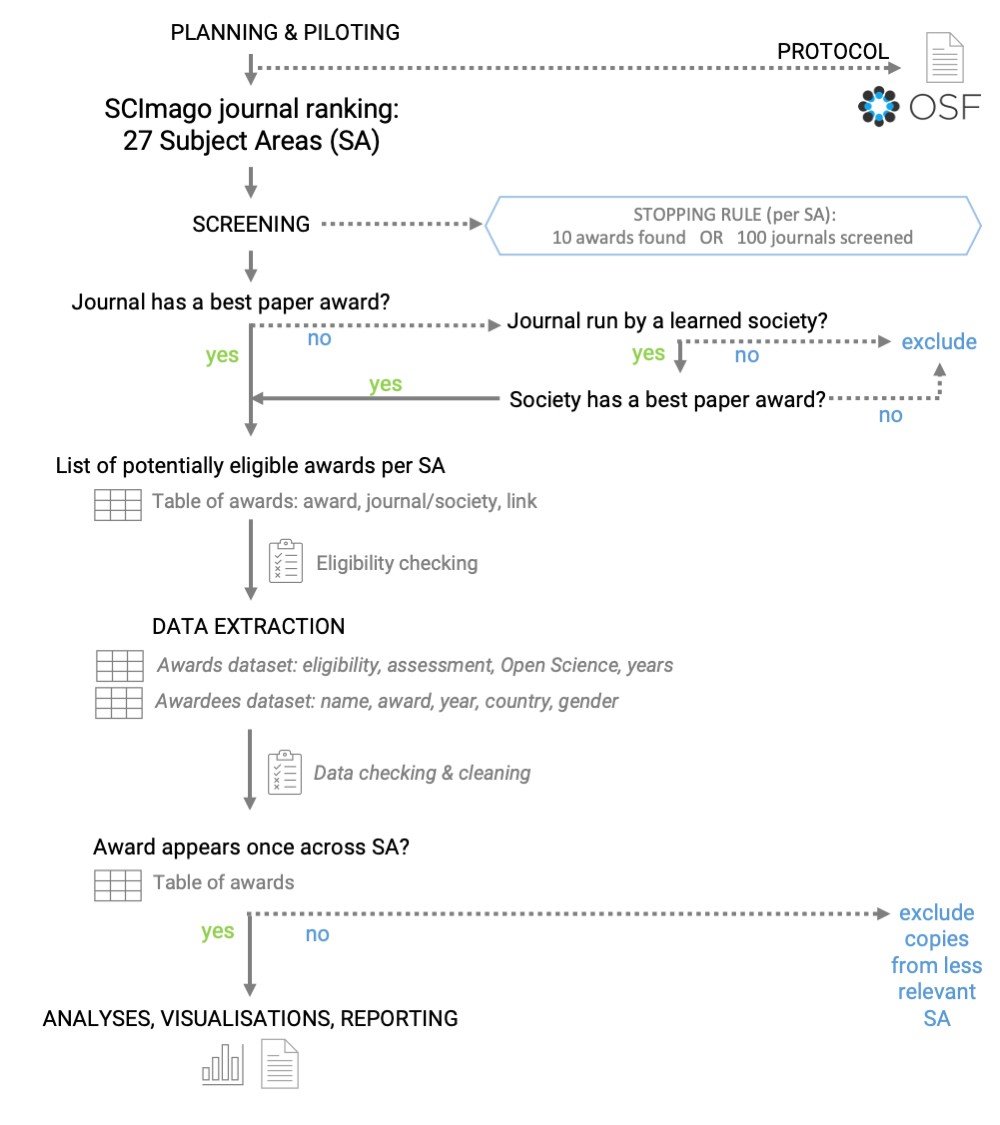
\includegraphics{../BP_awards_workflow_v2.png} Figure S1.\\
\textbf{Figure S1. project workflow}.

\hypertarget{project-aim-and-general-approach.}{%
\subsubsection{Project aim and general
approach.}\label{project-aim-and-general-approach.}}

``Best paper'' (or equivalent) awards are usually associated with
specific journals / societies / publishers. We aimed to conduct a
systematic-like search to collect a sample of highly regarded awards
(from top-ranking journals and societies) across a broad range of
disciplines. We conducted the process collaboratively and transparently
using shared Google Sheets documents (file copies were provided and
re-integrated for participants who were not able to access online Google
Docs).

The initial project description and contribution guidelines were
publicly available as GitHub pages:
\url{https://mlagisz.github.io/survey_best_paper_awards/}. Project
contributors were recruited via Open Science communities and
conferences. They helped to pilot the project procedures and provided
feedback on the project protocol, which was then updated to it second
version. roject contributors self-assigned to the individual project
tasks. Their actual contributions (completed tasks) were recorded on
Google Sheets. Detailed project procedures were shared as a dedicated
Project Manual on Google Docs. This document, with incorporated users'
feedback, is available at
\url{https://docs.google.com/document/d/1aw_HhKawpi264njGi--Ms-x-bOs_uQJBiOepQKE89pQ/edit?usp=sharing}.

\hypertarget{award-inclusion-criteria}{%
\subsubsection{Award inclusion
criteria}\label{award-inclusion-criteria}}

We followed pre-specified criteria outlined in the registered protocol
(\url{https://osf.io/7ez28}) to increase data consistency and enable
comparisons across disciplines:\\
1. We only included awards for a single published research contribution
in a format of a research article (theses / dissertations are allowed if
published as a journal article).\\
2. W only included awards managed by a journal, publisher, or a learned
society.\\
3. We excluded awards that are discontinued, and awards that are
restricted to applicants from underrepresented groups, e.g., women-only
/ minorities-only awards.

\hypertarget{search-and-screening}{%
\subsubsection{Search and screening}\label{search-and-screening}}

\begin{enumerate}
\def\labelenumi{\arabic{enumi}.}
\item
  Our starting point was from searching academic journals and
  societies/associations to identify those that award ``Best Paper''
  prizes. To do so, we first used journal lists from 27 SCImago Subject
  Areas (SA) rankings (SCImago Journal \& Country Rank (SJR) website at
  \url{https://www.scimagojr.com/journalrank.php}). To represent SAs
  evenly, we considered the top 100 journals from each SA list, or we
  will stop if we find 10 relevant awards before reaching this
  threshold.
\item
  During the intial screening, for each journal list representing a
  SSCImago Subject Area, we checked if journal websites or announcements
  include ``best paper'' awards , and if not, we checked if journals are
  run by learned societies (i.e.~are offciel journals of a given learned
  society/ies). If so, we also checked if a relevant learned society
  awards a ``best paper'' prize that fits in a given subject area being
  assessed. If a society awards multiple relevant awards in journals in
  the same subject area, we choose the one from our top 100 SA list or
  an award that appears to be most prestigious (e.g., with highest
  monetary value, oldest).
\item
  For each subject area, we collated a preliminary list of 10-15 awards
  that meet our selection criteria for data extraction. If some of these
  awards got excluded during data extraction, we went back to the
  screening stage for that subject area to find replacement awards until
  we had 10 awards that are eligible for inclusion, or we ran out of
  journals to screen within the top 100 SA list positions.
\end{enumerate}

\hypertarget{screening-cross-checking}{%
\subsubsection{Screening
cross-checking}\label{screening-cross-checking}}

\begin{enumerate}
\def\labelenumi{\arabic{enumi}.}
\item
  All screened journal lists from 27 Scimago Subject Areas (SA) rankings
  (\url{https://www.scimagojr.com}) were independently cross-checked to
  detect potential mistakes (it is easy to miss a note about awards on
  journals or organizational webpages, misinterpret eligibility of the
  award, etc.).
\item
  Project contributors self-assigned to one (or more) SCImago Subject
  Area (SA) - always different from the one they did initial SA
  screening.
\item
  The checking person confirmed if screening information and decision
  recorded by the initial screener is correct and accurate.
\item
  The checking person recorded in a new column (Award\_name\_extract)
  the name of the eligible award to be extracted and recorded any
  screening comments in additional columns.
\item
  Obvious mistakes were fixed and any unclear or disputable cases have
  been commented on and discussed before being resolved.
\end{enumerate}

\hypertarget{data-extraction}{%
\subsubsection{Data extraction}\label{data-extraction}}

\begin{enumerate}
\def\labelenumi{\arabic{enumi}.}
\item
  For each 27 Scimago Subject Areas (SA) ranking
  (\url{https://www.scimagojr.com}), we extracted data on max. 10 awards
  that meet our selection criteria.
\item
  For each award, its eligibility (as outlined in ``Selection
  criteria'') for inclusion was confirmed during data extraction, and if
  deemed not eligible, no further data was be extracted.
\item
  Using a pre-piloted Google Form, we extracted relevant data on each
  award from the websites (e.g., journals, societies, publishers) or
  other publicly available documents (e.g., instructions for
  applicants).
\item
  The extracted pre-specified data included information on the granting
  journal / publisher / society, award eligibility criteria, award
  assessment criteria, and source of information on the past awardees
  (full metadata is provided alongside the data files).
\item
  We archived web pages with award descriptions by saving them to .pdf
  files named after award names (as used in data extraction documents).
\item
  The second stap of data extraction focused on the identities and
  characteristics of the past participants. For collecting data on
  individual winners, we had a data collection directly on a Google
  Sheet. We only collect data on winners from years 2001-2022. This data
  was used to infer patterns related to individual winners' gender and
  country of affiliation. Specifically: Gender (binary: F = female, M =
  male, ? - unassigned) was be assigned to the past awardee names using
  information (pronouns, images, names) available on award websites,
  personal or institutional websites, or using
  \url{https://gender-api.com/}, with an accuracy threshold of
  \textgreater95 for assigning gender from first names. We noted
  instances of non-binary gender (not applicable) and also when we are
  unable to assign binary gender. Affiliation information (institution,
  country) was be assigned to past winners' names for the year when the
  award was received using information available on award websites,
  personal or institutional websites, or information in the awarded
  paper. Additional information was also recorded: links to the websites
  with relevant information, type of source of information (award page,
  award announcement, article, other), whether award is shared (more
  than one author from one winning paper), whether photo or bio are
  provided on award page or award announcement, reference information
  and DOI for winning article, any additional notes.
\end{enumerate}

\hypertarget{data-extraction-cross-checking}{%
\subsubsection{Data extraction
cross-checking}\label{data-extraction-cross-checking}}

\begin{enumerate}
\def\labelenumi{\arabic{enumi}.}
\item
  Extracted main award characteristics data (awarding body, description,
  etc.) has been independently cross-checked by a second researcher
  (i.e.~one that did not extract the data). Obvious mistakes were fixed
  and any unclear or disputable cases have been commented on and
  discussed before being resolved.
\item
  Extracted additional data (gender, affiliation country, and additional
  details on the award and winners) has been independently cross-checked
  by a second researcher (i.e.~one that did not extract the data).
  Obvious mistakes were fixed and any unclear or disputable cases have
  been commented on and discussed before being resolved.
\end{enumerate}

\hypertarget{data-processing-and-analyses---overview}{%
\subsubsection{Data processing and analyses -
overview}\label{data-processing-and-analyses---overview}}

The main steps were as follows:

\begin{enumerate}
\def\labelenumi{\arabic{enumi}.}
\tightlist
\item
  Uploading cross-checked meta-data, screening data and extracted data
  into R.\\
\item
  Creating meta-data tables (variable descriptions) for each data set.\\
\item
  Data pre-processing (e.g.~merging SA into a single data frame,
  removing excluded awards).\\
\item
  Summarising data sets via tabulation and filtering.\\
\item
  Creating figures for the supplementary materials - shown as in-text
  figures.\\
\item
  Creating figures for the main manuscript text - saced as . files.
\end{enumerate}

NOTE: Steps 3-6 were done for each data set in turn.\\
All code and results are provided below.

\hypertarget{loading-data}{%
\subsection{Loading data}\label{loading-data}}

\begin{itemize}
\tightlist
\item
  Load SCImago Subject Area -level data set and associated meta-data
  table.
\end{itemize}

\begin{Shaded}
\begin{Highlighting}[]
\CommentTok{\# accessing all the sheets }
\CommentTok{\#sheet\_names \textless{}{-} excel\_sheets(here("data", "scimagojr 2021  Subject Areas.xlsx"))}
\NormalTok{sheet\_names }\OtherTok{\textless{}{-}} \FunctionTok{excel\_sheets}\NormalTok{(}\FunctionTok{here}\NormalTok{(}\StringTok{"data"}\NormalTok{, }\StringTok{"scimagojr 2021  Subject Areas\_screening.xlsx"}\NormalTok{))}
\NormalTok{sheet\_names }\OtherTok{\textless{}{-}}\NormalTok{ sheet\_names[}\SpecialCharTok{{-}}\DecValTok{1}\NormalTok{]}\CommentTok{\#remove first sheet with meta{-}data}
\NormalTok{SA\_list\_all }\OtherTok{\textless{}{-}} \FunctionTok{lapply}\NormalTok{(sheet\_names, }\ControlFlowTok{function}\NormalTok{(x) \{}\FunctionTok{as.data.frame}\NormalTok{(}\FunctionTok{read\_excel}\NormalTok{(}\FunctionTok{here}\NormalTok{(}\StringTok{"data"}\NormalTok{, }\StringTok{"scimagojr 2021  Subject Areas.xlsx"}\NormalTok{), }\AttributeTok{sheet =}\NormalTok{ x))\}) }\CommentTok{\#read all sheets to list}
\FunctionTok{names}\NormalTok{(SA\_list\_all) }\OtherTok{\textless{}{-}}\NormalTok{ sheet\_names  }\CommentTok{\#rename list elements }
\CommentTok{\#lapply(SA\_list\_all, names) \#extract column names}
\CommentTok{\#View(do.call(rbind, lapply(SA\_list\_all, names))) \#View all column names as a table}
\CommentTok{\#unique(do.call(rbind, lapply(SA\_list\_all, names))) \#making sure all have same column names}
\NormalTok{SAdata }\OtherTok{\textless{}{-}} \FunctionTok{do.call}\NormalTok{(rbind, SA\_list\_all)}
\CommentTok{\#str(SAdata) \#one large data frame}
\CommentTok{\#names(SAdata)}
\FunctionTok{names}\NormalTok{(SAdata) }\OtherTok{\textless{}{-}} \FunctionTok{gsub}\NormalTok{(}\StringTok{" "}\NormalTok{,}\StringTok{"\_"}\NormalTok{, }\FunctionTok{names}\NormalTok{(SAdata)) }\CommentTok{\#change spaces to \_ in the column names}
\FunctionTok{names}\NormalTok{(SAdata) }\OtherTok{\textless{}{-}} \FunctionTok{gsub}\NormalTok{(}\StringTok{"}\SpecialCharTok{\textbackslash{}\textbackslash{}}\StringTok{."}\NormalTok{,}\StringTok{""}\NormalTok{, }\FunctionTok{names}\NormalTok{(SAdata)) }\CommentTok{\#remove . the column names}
\CommentTok{\#dim(SAdata)}
\NormalTok{SAdata }\OtherTok{\textless{}{-}}\NormalTok{ SAdata }\SpecialCharTok{\%\textgreater{}\%} \FunctionTok{drop\_na}\NormalTok{(Subject\_area)}
\CommentTok{\#table(is.na(SAdata$Title)) \#no empty journal names}

\NormalTok{SAmeta }\OtherTok{\textless{}{-}} \FunctionTok{read\_excel}\NormalTok{(}\FunctionTok{here}\NormalTok{(}\StringTok{"data"}\NormalTok{, }\StringTok{"scimagojr 2021  Subject Areas\_screening.xlsx"}\NormalTok{), }\AttributeTok{sheet =} \DecValTok{1}\NormalTok{, }\AttributeTok{skip =} \DecValTok{1}\NormalTok{) }\CommentTok{\#load Scimago SA meta{-}data}
\CommentTok{\#dim(SAmeta)}
\CommentTok{\#names(SAmeta)}
\end{Highlighting}
\end{Shaded}

\begin{itemize}
\tightlist
\item
  Load award-level data set and associated meta-data table.
\end{itemize}

\begin{Shaded}
\begin{Highlighting}[]
\CommentTok{\#BP load and prepare award{-}level meta{-}data}
\NormalTok{BPmeta }\OtherTok{\textless{}{-}} \FunctionTok{read\_excel}\NormalTok{(}\FunctionTok{here}\NormalTok{(}\StringTok{"data"}\NormalTok{, }\StringTok{"Survey{-}Best\_paper\_awards (Responses)\_SHAREDCOPY\_checked.xlsx"}\NormalTok{), }\AttributeTok{sheet =} \DecValTok{2}\NormalTok{, }\AttributeTok{skip =} \DecValTok{1}\NormalTok{) }\CommentTok{\#load main award \#BPmeta \textless{}{-} read\_excel("./data/Survey{-}Best\_paper\_awards (Responses)\_SHAREDCOPY\_checked.xlsx", sheet = 2, skip = 1) \#load main award meta{-}data}
\CommentTok{\#dim(BPmeta)}
\CommentTok{\#names(BPmeta)}

\DocumentationTok{\#\# load and prepare main extracted award{-}level data}
\NormalTok{BPdata }\OtherTok{\textless{}{-}} \FunctionTok{read\_excel}\NormalTok{(}\FunctionTok{here}\NormalTok{(}\StringTok{"data"}\NormalTok{,}\StringTok{"Survey{-}Best\_paper\_awards (Responses)\_SHAREDCOPY\_checked.xlsx"}\NormalTok{), }\AttributeTok{sheet =} \DecValTok{1}\NormalTok{) }\CommentTok{\#load main award data}
\CommentTok{\#BPdata \textless{}{-} read\_excel("./data/Survey{-}Best\_paper\_awards (Responses)\_SHAREDCOPY\_checked.xlsx", sheet = 1) \#load main award data}
\CommentTok{\#dim(BPdata)}
\CommentTok{\#names(BPdata)}

\CommentTok{\#BPdata \textless{}{-} select(BPdata, !starts\_with("...") ) \#remove last few empty columns}
\CommentTok{\#BPdata\_orig\_colnames \textless{}{-} names(BPdata) \#store original column names}
\CommentTok{\#BPdata$Award\_name \textless{}{-} gsub("\^{}The ", "", BPdata$Award\_name) \#remove "The" at the beginning of award names}
\FunctionTok{names}\NormalTok{(BPdata) }\OtherTok{\textless{}{-}} \FunctionTok{gsub}\NormalTok{(}\StringTok{" "}\NormalTok{,}\StringTok{"\_"}\NormalTok{, }\FunctionTok{names}\NormalTok{(BPdata)) }\CommentTok{\#change spaces to \_ in the column names}

\CommentTok{\#rename selected data columns}
\NormalTok{BPdata }\OtherTok{\textless{}{-}}\NormalTok{ BPdata }\SpecialCharTok{\%\textgreater{}\%} 
\FunctionTok{rename}\NormalTok{(}\AttributeTok{Extractor\_name =} \StringTok{"Name\_of\_the\_extracting\_person"}\NormalTok{,}
       \AttributeTok{Award\_name =} \StringTok{"Full\_name\_of\_the\_award"}\NormalTok{, }
       \AttributeTok{Journal\_name =} \StringTok{"Full\_name\_of\_the\_awarding\_journal"}\NormalTok{, }
       \AttributeTok{Award\_description =} \StringTok{"Paste\_the\_information\_text\_describing\_the\_award"}\NormalTok{, }
       \AttributeTok{Eligible =} \StringTok{"Confirm\_eligibility\_of\_the\_award"}\NormalTok{,}
       \AttributeTok{Awarding\_journal =} \StringTok{"Full\_name\_of\_the\_awarding\_journal"}\NormalTok{,}
       \AttributeTok{Awarding\_society =} \StringTok{"Full\_name\_of\_the\_awarding\_society"}\NormalTok{,}
       \AttributeTok{Awarding\_other =} \StringTok{"Full\_name\_of\_the\_awarding\_publisher/other\_body"}\NormalTok{,  }
       \AttributeTok{Career\_stage =} \StringTok{"Target\_career\_stage\_of\_eligible\_applicants"}\NormalTok{,}
       \AttributeTok{Flexible\_eligibility =} \StringTok{"Flexibility\_of\_the\_eligibility\_criteria"}\NormalTok{, }
       \AttributeTok{Assessors\_transparency =} \StringTok{"Assessor\_transparency"}\NormalTok{, }
       \AttributeTok{Open\_science =} \StringTok{"Valuing\_Open\_Science"}\NormalTok{,  }
       \AttributeTok{Self\_nomination =} \StringTok{"Self{-}nomination\_allowed"}
\NormalTok{       )}
\CommentTok{\#names(BPdata)}

\DocumentationTok{\#\#check for rows with empty "Scimago Subject Area" values}
\FunctionTok{table}\NormalTok{(}\FunctionTok{is.na}\NormalTok{(BPdata}\SpecialCharTok{$}\NormalTok{Scimago\_Subject\_Area)) }\CommentTok{\#4 rows from pilot screening}
\end{Highlighting}
\end{Shaded}

\begin{verbatim}
## 
## FALSE  TRUE 
##   264     4
\end{verbatim}

\begin{Shaded}
\begin{Highlighting}[]
\DocumentationTok{\#\#remove rows with pilot extractions and empty "Scimago Subject Area" values}
\NormalTok{BPdata }\OtherTok{\textless{}{-}}\NormalTok{ BPdata[}\SpecialCharTok{!}\FunctionTok{is.na}\NormalTok{(BPdata}\SpecialCharTok{$}\NormalTok{Scimago\_Subject\_Area), ]}

\CommentTok{\#remove awards that were duplicate{-}extracted and excluded at extraction stages}
\NormalTok{BPdata }\OtherTok{\textless{}{-}}\NormalTok{ BPdata[BPdata}\SpecialCharTok{$}\NormalTok{Row\_excluded }\SpecialCharTok{==} \DecValTok{0}\NormalTok{, ]}
\FunctionTok{dim}\NormalTok{(BPdata) }\CommentTok{\#223 rows left}
\end{Highlighting}
\end{Shaded}

\begin{verbatim}
## [1] 223  54
\end{verbatim}

\begin{Shaded}
\begin{Highlighting}[]
\DocumentationTok{\#\#NOTE: total of 41 rows were removed as duplicates: 18 awards were doubly{-} or triply{-} extracted (total 18 out of 223 = 8\%)}

\CommentTok{\#create new variable for awards with description or without}
\NormalTok{BPdata}\SpecialCharTok{$}\NormalTok{Descr\_available }\OtherTok{\textless{}{-}} \FunctionTok{fct\_collapse}\NormalTok{(BPdata}\SpecialCharTok{$}\NormalTok{Open\_science,}
  \AttributeTok{available =} \FunctionTok{c}\NormalTok{(}\StringTok{"no"}\NormalTok{, }\StringTok{"yes"}\NormalTok{),}
  \StringTok{"not available"} \OtherTok{=} \StringTok{"not available"}
\NormalTok{)}
\end{Highlighting}
\end{Shaded}

\begin{itemize}
\tightlist
\item
  Load winners-level data set and associated meta-data table.
\end{itemize}

\begin{Shaded}
\begin{Highlighting}[]
\CommentTok{\#load individual winners data}
\NormalTok{BPindiv }\OtherTok{\textless{}{-}} \FunctionTok{read\_csv}\NormalTok{(}\FunctionTok{here}\NormalTok{(}\StringTok{"data"}\NormalTok{, }\StringTok{"BP\_awards\_lists\_SHAREDCOPY {-} indiv\_winners\_20230717.csv"}\NormalTok{), }\AttributeTok{skip =} \DecValTok{1}\NormalTok{) }\CommentTok{\#load individual winners data}
\end{Highlighting}
\end{Shaded}

\begin{verbatim}
## Rows: 1083 Columns: 22
## -- Column specification --------------------------------------------------------
## Delimiter: ","
## chr (20): award_SA, award_name, award_link, individual, awardee_name, awarde...
## dbl  (2): record_count, award_year
## 
## i Use `spec()` to retrieve the full column specification for this data.
## i Specify the column types or set `show_col_types = FALSE` to quiet this message.
\end{verbatim}

\begin{Shaded}
\begin{Highlighting}[]
\CommentTok{\#dim(BPindiv)}
\CommentTok{\#names(BPindiv)}

\CommentTok{\#load individual winners meta{-}data}
\NormalTok{BPindiv\_meta }\OtherTok{\textless{}{-}} \FunctionTok{read\_csv}\NormalTok{(}\FunctionTok{here}\NormalTok{(}\StringTok{"data"}\NormalTok{, }\StringTok{"BP\_awards\_lists\_SHAREDCOPY {-} indiv\_winners\_meta{-}data.csv"}\NormalTok{), }\AttributeTok{skip =} \DecValTok{1}\NormalTok{) }\CommentTok{\#load individual winners data}
\end{Highlighting}
\end{Shaded}

\begin{verbatim}
## Rows: 22 Columns: 3
## -- Column specification --------------------------------------------------------
## Delimiter: ","
## chr (3): column name, description, data type [options]
## 
## i Use `spec()` to retrieve the full column specification for this data.
## i Specify the column types or set `show_col_types = FALSE` to quiet this message.
\end{verbatim}

\begin{Shaded}
\begin{Highlighting}[]
\CommentTok{\#dim(BPindiv\_meta)}
\CommentTok{\#names(BPindiv\_meta)}
\end{Highlighting}
\end{Shaded}

\begin{itemize}
\tightlist
\item
  Load country-level productivity SCImago data set and create associated
  meta-data table.
\end{itemize}

\begin{Shaded}
\begin{Highlighting}[]
\CommentTok{\#load SCImago 2021 country productivity (documents) data downloaded from https://www.scimagojr.com/countryrank.php?year=2021\&min=0\&min\_type=it}
\NormalTok{COprod }\OtherTok{\textless{}{-}} \FunctionTok{read\_csv}\NormalTok{(}\FunctionTok{here}\NormalTok{(}\StringTok{"data"}\NormalTok{, }\StringTok{"scimagojr country rank 2021.csv"}\NormalTok{), }\AttributeTok{skip =} \DecValTok{0}\NormalTok{) }\CommentTok{\#load data}
\end{Highlighting}
\end{Shaded}

\begin{verbatim}
## Rows: 235 Columns: 9
## -- Column specification --------------------------------------------------------
## Delimiter: ","
## chr (2): Country, Region
## dbl (7): Rank, Documents, Citable documents, Citations, Self-citations, Cita...
## 
## i Use `spec()` to retrieve the full column specification for this data.
## i Specify the column types or set `show_col_types = FALSE` to quiet this message.
\end{verbatim}

\begin{Shaded}
\begin{Highlighting}[]
\CommentTok{\#dim(COprod)}
\CommentTok{\#names(COprod)}

\CommentTok{\#create meta{-}data with columns:         data type [options]}
\NormalTok{COprod\_meta }\OtherTok{\textless{}{-}} \FunctionTok{tibble}\NormalTok{(}\StringTok{"column name"} \OtherTok{=} \FunctionTok{names}\NormalTok{(COprod), }
                      \StringTok{"description"} \OtherTok{=} \FunctionTok{c}\NormalTok{(}\StringTok{"Rank of a given country across all Scimago Subject Areas."}\NormalTok{,}
                                        \StringTok{"Country name."}\NormalTok{,}
                                        \StringTok{"Country location classification into one of the eight SCImago Major World Regions."}\NormalTok{,}
                                        \StringTok{"Number of documents associated with a goven country published in 2021."}\NormalTok{,}
                                        \StringTok{"Number of citable documents associated with a goven country published in 2021."}\NormalTok{,}
                                        \StringTok{"Number of citations to documents associated with a goven country published in 2021."}\NormalTok{,}
                                        \StringTok{"Number of self{-}citations to documents associated with a goven country published in 2021."}\NormalTok{,}
                                        \StringTok{"Number of citations per document associated with a goven country published in 2021."}\NormalTok{,}
                                        \StringTok{"H index of a country in 2021."}\NormalTok{ ),}
                      \StringTok{"data type [options]"} \OtherTok{=} \FunctionTok{c}\NormalTok{(}\StringTok{"integer"}\NormalTok{,}
                                                \StringTok{"free text"}\NormalTok{,}
                                                \StringTok{"free text"}\NormalTok{,}
                                                \StringTok{"integer"}\NormalTok{,}
                                                \StringTok{"integer"}\NormalTok{,}
                                                \StringTok{"integer"}\NormalTok{,}
                                                \StringTok{"integer"}\NormalTok{,}
                                                \StringTok{"numeric"}\NormalTok{,}
                                                \StringTok{"integer"}
\NormalTok{                                                ))}
\CommentTok{\#dim(COprod\_meta)}
\CommentTok{\#names(COprod\_meta)}
\end{Highlighting}
\end{Shaded}

\hypertarget{meta-data-tables}{%
\subsection{Meta-data tables}\label{meta-data-tables}}

\hypertarget{table-s1.}{%
\paragraph{Table S1.}\label{table-s1.}}

\emph{Meta-data for the SCImago journal rankings by Subject Areas
dataset}.

\begin{Shaded}
\begin{Highlighting}[]
\CommentTok{\# making a scrollable table}
\FunctionTok{kable}\NormalTok{(SAmeta, }\StringTok{"html"}\NormalTok{) }\SpecialCharTok{\%\textgreater{}\%}
  \FunctionTok{kable\_styling}\NormalTok{(}\StringTok{"striped"}\NormalTok{, }\AttributeTok{position =} \StringTok{"left"}\NormalTok{) }\SpecialCharTok{\%\textgreater{}\%}
  \FunctionTok{scroll\_box}\NormalTok{(}\AttributeTok{width =} \StringTok{"100\%"}\NormalTok{, }\AttributeTok{height =} \StringTok{"500px"}\NormalTok{)}
\end{Highlighting}
\end{Shaded}

column name

description

data type {[}options{]}

Subject\_area

Name of the Scimago Subject Area (SA) representing 27 major thematic
categories.

categorical {[}one of 27 Subject Areas{]}

Rank

Rank of a given Journal within a given Scimago Subject Area.

integer

Sourceid

Unique ID for the journal.

integer

Title

Name of the journal.

free text

Reviewer\_name

Name of a person who reviews the journal trying to find associated
eligible awards.

free text

Link\_journal

Year when award was won/announced for a give individual winner, as
reported on the award page or other documents with winner information.

web link

Society\_name

Name of a person who won the award, as reported on the award page or
other documents with winner information.

free text

Has\_relevant\_award

Gender assigned to an individual past awardee names using information
from pronouns, images, names) available on award websites, personal or
institutional websites, or from first names.

categorical {[}yes; no{]}

Link\_award

Main source of information for assigning gender. Order of preference:
pronouns, photo, name.

web link

Notes\_award

Affiliation institution (usually university) assigned to a winner when
the award was received using information available on award websites,
personal or institutional websites, or information in the awarded paper.

free text

Checker\_name

Name of the person who cross-checked a given row of screening data.

free text

Check\_pass

Main source of the winner's affiliation information (institution,
country) for the year when the award was received or announced.

categorical {[}yes; no{]}

Check\_notes

Any comments for awardee, e.g.~award sub-category, or link to additional
info from Internet searches.

free text

Award\_name\_extract

Whether the award is shared with other authors of the same article.

categorical {[}yes; no{]}

Extract

Whether a bio/profile of the winner is shown on the award
page/announcement (with more extended information than affiliation
information only).

categorical {[}yes; no{]}

Award\_extractor\_name

Name of the person who extracted award data .

categorical {[}yes; no{]}

Extracted

Whether a given award has been extracted.

categorical {[}yes; no{]}

Comments

Anny comments regarding screened and extracted data in a given row.

free text

Archived

DOI of the winning paper. DOI code in a format starting with ``10.''.

DOI

Issn

ISSN number of teh journal

free text

SJR

SCImago Journal Rank indicator expresses the average number of weighted
citations received in the selected year by the documents published in
the selected journal in the three previous years, i.e.~weighted
citations received in year X to documents published in the journal in
years X-1, X-2 and X-3

free text

SJR Best Quartile

Anny comments regarding extracted data in a given row.

categorical {[}Q1; Q2; Q3; Q4{]}

H index

The h index expresses the journal's number of articles (h) that have
received at least h citations. It quantifies both journal scientific
productivity and scientific impact and it is also applicable to
scientists, countries, etc.

number

Total Docs. (2021)

Output of the selected period. All types of documents are considered,
including citable and non citable documents.

integer

Total Docs. (3years)

Published documents in the three previous years (selected year documents
are excluded), i.e.when the year X is selected, then X-1, X-2 and X-3
published documents are retrieved. All types of documents are
considered, including citable and non citable documents.

integer

Total Refs.

Total number of all the bibliographical references in a journal in the
selected period.

integer

Total Cites (3years)

Number of citations received in the seleted year by a journal to the
documents published in the three previous years, --i.e.~citations
received in year X to documents published in years X-1, X-2 and X-3. All
types of documents are considered.

integer

Citable Docs. (3years)

Number of citable documents published by a journal in the three previous
years (selected year documents are excluded). Exclusively articles,
reviews and conference papers are considered.

integer

Cites / Doc. (2years)

Average citations per document in a 2 year period. It is computed
considering the number of citations received by a journal in the current
year to the documents published in the two previous years,
--i.e.~citations received in year X to documents published in years X-1
and X-2.

number

Ref. / Doc.

References per Document is the average number of references per document
in the selected year.

number

Country

Country where journal is indexed by Scopus.

categorical

Region

Eight Major World Regions in used to facilitate sectorial analyses.

categorical

Publisher

name of teh journal publisher.

free text

Coverage

Year range for which publication data is available on Scopus (?).

free text

Categories

Tags for relevant 309 specific subject categories according to Scopus®
Classification.

categorical

\hypertarget{table-s2.}{%
\paragraph{Table S2.}\label{table-s2.}}

\emph{Meta-data for the Best Paper awards dataset}.

\begin{Shaded}
\begin{Highlighting}[]
\CommentTok{\# making a scrollable table}
\FunctionTok{kable}\NormalTok{(BPmeta, }\StringTok{"html"}\NormalTok{) }\SpecialCharTok{\%\textgreater{}\%}
  \FunctionTok{kable\_styling}\NormalTok{(}\StringTok{"striped"}\NormalTok{, }\AttributeTok{position =} \StringTok{"left"}\NormalTok{) }\SpecialCharTok{\%\textgreater{}\%}
  \FunctionTok{scroll\_box}\NormalTok{(}\AttributeTok{width =} \StringTok{"100\%"}\NormalTok{, }\AttributeTok{height =} \StringTok{"500px"}\NormalTok{)}
\end{Highlighting}
\end{Shaded}

column name

description

data type {[}options{]}

Timestamp

System-recorded data and time of when the given row of data was
submitted via the Google Form.

time

Name of the extracting person

Name of the extracting person: Please use your name in one consistent
form (should be matching the name you gave us on EOI and recorded on
GoogleSheet for award screening). It is best to always use your first
and last name, to avoid confusion.

free text

Scimago Subject Area

Scimago Subject Area: Record name of the Scimago Subject Area (SA) you
are doing extractions for - as in the Subject\_area column in the
GoogleSheet with journal and awards lists. Should be exactly as used in
the original list of Subject Areas.

categorical {[}one of 27 Subject Areas{]}

Full name of the award

Full name of the award: Record specific award name, as in the
Award\_name\_extract column in the GoogleSheet with journal and awards
lists.

free text

Source of the information on the award

Source of the information on the award: Ideally, enter a link to an
online page/document with information on award eligibility and
assessment criteria. If not available, could be also a link to any
document describing the award. If you cannot find any information about
the award enter ``NA''. You can paste more than one link separated by
``;''.

weblink

Paste the information text describing the award

Paste the information text describing the award: Ideally, copy and paste
the section of the online page/document with information on award
eligibility and assessment criteria only. This description text will be
used for text-mining analyses. Do not copy and paste list of past
winners or generic information about the journal or society. Do not copy
and paste any images. If you cannot find any information about the award
enter ``NA''.

free text

Confirm eligibility of the award

Confirm eligibility of the award: · This award is for a single published
research contribution in a format of a research article (theses /
dissertation are allowed if published as a journal article). · This
award is managed by a journal, publisher, or a learned society. · This
award is NOT discontinued or restricted to applicants from
underrepresented groups, e.g., women-only / minorities-only. Options:
yes (eligible award), no (not eligible - make note on the reasons below
and enter NA to the following compulsory questions, then submit),
unclear (make note on the reasons below)

categorical {[}yes; no; unclear{]}

Comment on the award eligibility

Comment on the award eligibility: Any comments, e.g.~reasons for
excluding this award.

free text

Full name of the awarding journal

Full name of the awarding journal: Record if award is associated with a
specific journal. Enter ``NA'' if not associated with a specific
journal.

free text

Full name of the awarding society

Full name of the awarding society: Record if award is associated with a
specific society. Enter ``NA'' if not associated with a specific
society.

free text

Full name of the awarding publisher/other body

Full name of the awarding publisher/other body: Record if award is
associated with a specific publisher (group of journals) or awarding
organisation other than learned society or journal. Enter ``NA'' if not
associated with a specific publisher.

free text

Comment on the awarding body

Comment on the awarding body: Any comments, e.g.~if more than one
journal considered for the award.

free text

Award cash

Award cash: Code whether there is any cash coming with the award. -
Select ``yes'' if award description mentions any cash given to the
winners. - Select ``no'' if award description does not mention any cash
given to the winners. Travel awards, publishing discounts, plenary
talks, etc. do not count as cash awards. - Select ``not available'' if
there is no page/document describing the award (e.g.~only the list of
winners is publicly published). NOTE: In the next question
(``Inclusivity phrasing'') copy and paste relevant text from the award
document or make a note if no such document/information is available.
Options: yes, no, not available.

free text

Comment on the award cash

Comment on the award cash: Add comments on cash amount, if provided, and
note any other benefits winners receive, as relevant (e.g., travel
awards, publishing discounts, plenary talks)

free text

Target career stage of eligible applicants

Target career stage of eligible applicants, as stated in the award
information: As stated in the award information. More than one choice is
possible. If it is for any paper in a journal/s, select ``any career
stage''. Options: student, early-career, mid-career, any career stage,
unclear.

categorical {[}student; early-career; mid-career; any career stage;
unclear{]}

Comment on the career stage

Comment on the career stage: Any comments, e.g.~paste the phrasing of
who is eligible for the award.

free text

Flexibility of the eligibility criteria

Flexibility of the eligibility criteria: Code whether explicitly
allowing for career interruptions in eligibility timeframes: - Select
``not applicable'' if description only states that published research
has to be performed while studying for a degree OR if there is no
eligibility limit in terms of years since an event (e.g.~a PhD or
author's age. - Select ``yes'' if the description says that there is an
eligibility limit of years after a degree to apply for the. award and
this limit can be extended in special cases''. - Select ``no'' if the
description says that there is an eligibility limit of years after a
degree to apply for the award but it does not mention that this limit
can be extended in special cases. - Select ``not available'' if there is
no page/document describing the award (e.g.~only the list of winners is
publicly published). NOTE: In the next question (``Eligibility
phrasing'') copy and paste relevant text from the award document or make
a note if no such document/information is available. Options: yes, no,
not applicable, not available.

categorical {[}yes; no; not applicable; not available{]}

Eligibility phrasing

Eligibility phrasing: Wording of the eligibility criteria in relation to
career stage in the relevant documentation, if available.

free text

Inclusivity statement

Inclusivity statement: Code whether underrepresented/minority groups are
encouraged to apply for the award (this does not mean that the award is
restricted to underrepresented groups, e.g., women-only) or award
information includes declarations of commitment to equity / diversity /
inclusivity (EDI): - Select ``yes'' if award description mentions
underrepresented/minority groups or EDI. - Select ``no'' if award
description does not mention anything about underrepresented/minority
groups or EDI. - Select ``not available'' if there is no page/document
describing the award (e.g.~only the list of winners is publicly
published). NOTE: Extract this information from award descriptions only
- do not include information from other documents not directly related
to the award, e.g.~journal/society/institutional policies or mission
statements. In the next question (``Inclusivity phrasing'') copy and
paste relevant text from the award document or make a note if no such
document/information is available.

categorical {[}yes; no; not available{]}

Inclusivity phrasing

Inclusivity phrasing: Wording of the inclusivity statement in the
relevant documentation, if available.

free text

Assessor transparency

Assessor transparency: Code whether information is provided on who will
be conducting assessments of candidate papers (for example, that
editors-in-chief will be deciding): - Select ``yes'' if information is
provided, e.g.~names, or stating that journal editors will be doing
this, or mentioning specific existing committee that is described
somewhere else (e.g.~on a society webpage). - Select ``no'' if
description does not mention any information on the assessors. - Select
``not available'' if there is no page/document describing the award
(e.g.~only the list of winners is publicly published). In the next
question (``Assessor phrasing'') copy and paste relevant text from the
award document or make a note if no such document/information is
available.

categorical {[}yes; no; not available{]}

Assessor phrasing

Assessor phrasing: Wording of the information on who will be conducting
the assessments, if available.

free text

Process transparency

Process transparency: Code whether breakdown of the applicants /
candidates by gender or geographic region is publicly available: -
Select ``yes'' if such information is provided (e.g.~on a society
webpage). - Select ``no'' if such information is not provided. - Select
``not available'' if there is no page/document describing the award
(e.g.~only the list of winners is publicly published). NOTE: In the next
question (``Process phrasing'') copy and paste relevant text from the
award document or make a note if no such document/information is
available. Options: yes, no, not available.

categorical {[}yes; no; not available{]}

Process phrasing

Process phrasing: Wording of the information on the transparency of the
process, e.g.~if breakdown of the applicants / candidates by gender or
geographic region is publicly available.

free text

Feedback availability

Feedback availability: Code whether award information included an offer
of constructive feedback for unsuccessful applicants: - Select ``yes''
if such feedback can be provided (e.g.~on request). - Select ``no'' if
such feedback is not provided or not mentioned. - Select ``not
available'' if there is no page/document describing the award (e.g.~only
the list of winners is publicly published). NOTE: In the next question
(``Feedback phrasing'') copy and paste relevant text from the award
document or make a note if no such document/information is available.
Options: yes, no, not available.

categorical {[}yes; no; not available{]}

Feedback phrasing

Feedback phrasing: Wording of the information on whether/how feedback
will be provided, if available.

free text

Criteria transparency

Criteria transparency: Code whether assessment criteria are detailed
(more than one vague sentence) or vague (often one vague sentence,
e.g.~``assessed on innovation and novelty''): - Select ``yes'' if
assessment criteria are more than one vague sentence (e.g., mentions
things like readability of the language, sample size, performing
alternative tests/analyses to check robustness of the results, sharing
data or code, registering the study/protocol - whatever is relevant to a
given research field). - Select ``no'' if assessment criteria are only
one vague sentence (e.g.~award is for ``best paper'', ``outstanding
contribution'', ``excellent research'', ``novel insights'', etc.). -
Select ``not available'' if there is no page/document describing the
award (e.g.~only the list of winners is publicly published). NOTE: In
the next question (``Criteria phrasing'') copy and paste relevant text
from the award document or make a note if no such document/information
is available. Options: yes, no, not available.

categorical {[}yes; no; not available{]}

Criteria phrasing

Criteria phrasing: Wording of the information on the assessment
criteria, if available.

NA

Valuing Open Science

Valuing Open Science: Code whether any Open Science practices (data,
code, materials sharing, preregistration, transparency of reporting,
etc.) are explicitly included in the assessment criteria: - Select
``yes'' if award description mentions valuing any of the Open Science
practices (e.g., sharing data or code, registering the study/protocol,
performing replication studies - whatever is relevant to a given
research field). - Select ``no'' if the award description does not
mention valuing any of the Open Science practices. - Select ``not
available'' if there is no page/document describing the award (e.g.~only
the list of winners is publicly published). NOTE: In the next question
(``Valuing Open Science phrasing'') copy and paste relevant text from
the award document or make a note if no such document/information is
available. Options: yes, no, not available.

categorical {[}yes; no; not available{]}

Valuing Open Science phrasing

Valuing Open Science phrasing: Wording of the information on the
assessment criteria valuing Open Science practices, if available.

free text

Self-nomination allowed

Self-nomination allowed: Code whether candidates can self-nominate for
the award. - Select ``yes'' if the award description explicitly mentions
that candidates can self-nominate. - Select ``no'' if the award
description states that candidates/papers need to be nominated by
somebody else or does not explicitly mention that candidates can
self-nominate. - Select ``not available'' if there is no page/document
describing the award (e.g.~only the list of winners is publicly
published). NOTE: In the next question (``Self-nomination phrasing'')
copy and paste relevant text from the award document or make a note if
no such document/information is available. Options: yes, no, not
available,

categorical {[}yes; no; not available{]}

Self-nomination phrasing

Self-nomination phrasing: Wording of the information on how to nominate
(e.g., using a checkbox on the manuscript submission form), if
available.

free text

Letter required

Letter required: Code whether candidates are required to provide
nomination/recommendation letter/s: - Select ``yes'' if award
description explicitly mentions that candidates have to provide
nomination or support letters from others. - Select ``no'' if the award
description states that candidates/papers do not need to provide letters
from somebody else or does not explicitly mention anything about such
letters. - Select ``not available'' if there is no page/document
describing the award (e.g.~only the list of winners is publicly
published). NOTE: In the next question (``Letter requirement phrasing'')
copy and paste relevant text from the award document or make a note if
no such document/information is available. Options: yes, no, not
available.

categorical {[}yes; no; not available{]}

Letter requirement phrasing

Letter requirement phrasing: Wording of the information on the
requirement for written nominations / reference letters, if available.

free text

Awardee list source

Awardee list source: Source of the information on the past winners -
paste a link to a webpage, file name, personal information, etc.,
showing a list of past winners (any year span). Write ``not available''
if no such list exists.

weblink

Awardee list most recent year

Awardee list most recent year: The most recent year for which
information on past awardees is available (enter whole number,
e.g.~2022). Leave empty if no such list exists.

integer

Awardee list earliest year

Awardee list earliest year: The earliest year for which information on
past awardees is available (enter whole number, e.g.~1999). Leave empty
if no such list exists.

integer

Comments on awardees list

Comments on awardees list: Any comments for awardees list, e.g.~if
Internet searches might be needed to locate announcements with the names
of the past winners.

free text

Comments\_general

Comments\_general: Any other notes and comments on issues, assumptions,
or seeking additional information from the award committees / contacts.

free text

Checked

Whether a given row of extracted data has been cross-checked.

categorical {[}yes; no{]}

Checker\_name

Name of the person who cross-checked a given row of extracted data.

free text

Checker\_comments

Anny comments regarding extracted data in a given row.

free text

Row\_excluded

Whether a given row of extracted data has been cross-checked.

integer {[}1 = yes; 0 = no{]}

Award\_individual

Whether a given award recognises individual (selected) authors rather
than all authors of a winning paper.

categorical {[}yes; no{]}

Award\_impact\_metrics\_mentioned

Whether award criteria mention impact metrics (number of citations,
downloads) as basis of winner selection.

categorical {[}yes; no{]}

Award\_impact\_metrics\_only

Whether impact metrics (number of citations, downloads) ar the sole
basis of winner selection.

categorical {[}yes; no{]}

Award\_impact\_metrics\_comment

Quote relevent sections of award description if impact metrics are
mentioned. Add any comments regarding award criteria and impact metrics.

free text

Award\_contact\_provided

Whether specific contact information (email) is provided on the award
webpage or publicly available application/description documents.

categorical {[}yes; no{]}

Award\_integrity\_mentioned

Whether award description states how potential conflictes of interests
will be managed

categorical {[}yes; no; not available{]}

Award\_integrity\_comment

Quote relevent sections of award description on how potential conflicts
of interests will ba managed.

free text

Award\_cash\_max\_USD\_pperson

The maximum reported amount of cash awarded per winning paper,
recalculated online into USD.

Integer

N\_winners\_extracted

Number of individual winners from years 2001-2022 extracted for this
awards (in indiv\_winners data set).

Integer

Archived\_files

Whether award website and over information have been archived as pdf
files in the dedicated project folder.

categorical {[}yes; no{]}

Comment\_extraction

Anny comments regarding extracted data in a given row.

free text

\hypertarget{table-s3.}{%
\paragraph{Table S3.}\label{table-s3.}}

\emph{Meta-data for the individual winners dataset}.

\begin{Shaded}
\begin{Highlighting}[]
\CommentTok{\# making a scrollable table}
\FunctionTok{kable}\NormalTok{(BPindiv\_meta, }\StringTok{"html"}\NormalTok{) }\SpecialCharTok{\%\textgreater{}\%}
  \FunctionTok{kable\_styling}\NormalTok{(}\StringTok{"striped"}\NormalTok{, }\AttributeTok{position =} \StringTok{"left"}\NormalTok{) }\SpecialCharTok{\%\textgreater{}\%}
  \FunctionTok{scroll\_box}\NormalTok{(}\AttributeTok{width =} \StringTok{"100\%"}\NormalTok{, }\AttributeTok{height =} \StringTok{"500px"}\NormalTok{)}
\end{Highlighting}
\end{Shaded}

column name

description

data type {[}options{]}

award\_SA

Name of the Scimago Subject Area (SA) you are doing extractions for - as
in the Subject\_area column in the GoogleSheet with journal and awards
lists. Should be exactly as used in the original list of Subject Areas.

categorical {[}one of 27 Subject Areas{]}

record\_count

Subsequent numbers for counting extracted winners within each award.

integer

award\_name

Name of the award - as in the Award\_name column in the main GoogleSheet
with awards main data extraction.

free text

award\_link

Weblink to the main Internet page with award description / information.

weblink

individual

Whether an award is individual or article-focused. Individual awards are
defined as awards that are usually not shared equally between all
article authors. For example the award names as a winner only the ECR
authors or only the first author (unless there are more than one
ECR/first authors who contributed equally).

categorical {[}yes; no{]}

award\_year

Year when award was won/announced for a give individual winner, as
reported on the award page or other documents with winner information.

integer

awardee\_name

Name of a person who won the award, as reported on the award page or
other documents with winner information.

free text

awardee\_gender

Gender assigned to an individual past awardee names using information
from pronouns, images, names) available on award websites, personal or
institutional websites, or from first names.

categorical {[}F = female; M = male; ? - unassigned{]}

gender\_source

Main source of information for assigning gender. Order of preference:
pronouns, photo, name.

categorical {[}pronouns; photo; name{]}

affiliation\_institution

Affiliation institution (usually university) assigned to a winner when
the award was received using information available on award websites,
personal or institutional websites, or information in the awarded paper.

free text

affiliation\_country

Affiliation country assigned to a past winner for the year when the
award was received using information available on award websites,
personal or institutional websites, or information in the awarded paper.

free text

affiliation\_info\_source

Main source of the winner's affiliation information (institution,
country) for the year when the award was received or announced.

categorical {[}award page; award announcement; article; other{]}

awardee\_comment1

Any comments for awardee, e.g.~award sub-category, or link to additional
info from Internet searches.

free text

shared

Whether the award is shared with other authors of the same article.

categorical {[}yes; no{]}

awardee\_profile\_shown

Whether a bio/profile of the winner is shown on the award
page/announcement (with more extended information than affiliation
information only).

categorical {[}yes; no{]}

awardee\_photo\_shown

Whether a photo of the winner is shown on the award page/announcement.

categorical {[}yes; no{]}

awardee\_comment2

Any other comments on the awardee or awarded paper, e.g.~award
sub-category, or link to additional info from Internet searches.

free text

awarded\_paper\_ref

Bibliographic reference of the winning paper.

free text {[}reference in any long format{]}

awarded\_paper\_doi

DOI of the winning paper. DOI code in a format starting with ``10.''.

DOI

checked

Whether a given row of extracted data has been cross-checked.

categorical {[}yes; no{]}

checker\_name

Name of the person who cross-checked a given row of extracted data.

free text

checker\_comment

Anny comments regarding extracted data in a given row.

free text

\hypertarget{supplementary-results}{%
\section{Supplementary Results}\label{supplementary-results}}

\hypertarget{characteristics-of-scimago-subject-area-sa-journal-lists-and-screening-data}{%
\subsection{Characteristics of SCImago Subject Area (SA) journal lists
and screening
data}\label{characteristics-of-scimago-subject-area-sa-journal-lists-and-screening-data}}

\hypertarget{number-of-journals-per-scimago-subject-area}{%
\subsubsection{Number of journals per SCImago Subject
Area}\label{number-of-journals-per-scimago-subject-area}}

\begin{Shaded}
\begin{Highlighting}[]
\DocumentationTok{\#\#count journals per SA}
\CommentTok{\# count\_j\_perSA \textless{}{-} SAdata \%\textgreater{}\%}
\CommentTok{\#     count(Subject\_area) \%\textgreater{}\%}
\CommentTok{\#     arrange(desc(n)) }

\CommentTok{\#table(SAdata$Subject\_area)}
\CommentTok{\#min(table(SAdata$Subject\_area))}
\CommentTok{\#max(table(SAdata$Subject\_area))}

\CommentTok{\#all SA as a simple barplot}
\NormalTok{SAdata }\SpecialCharTok{\%\textgreater{}\%} 
  \CommentTok{\#filter(!is.na(Subject\_area)) \%\textgreater{}\% }
  \FunctionTok{count}\NormalTok{(Subject\_area) }\SpecialCharTok{\%\textgreater{}\%}
  \FunctionTok{arrange}\NormalTok{(Subject\_area) }\SpecialCharTok{\%\textgreater{}\%}
  \FunctionTok{ggplot}\NormalTok{(}\FunctionTok{aes}\NormalTok{(}\AttributeTok{x =} \FunctionTok{reorder}\NormalTok{(Subject\_area, }\FunctionTok{desc}\NormalTok{(Subject\_area)), }\AttributeTok{y =}\NormalTok{ n)) }\SpecialCharTok{+}
  \FunctionTok{geom\_bar}\NormalTok{(}\AttributeTok{stat =} \StringTok{"identity"}\NormalTok{, }\AttributeTok{position =} \FunctionTok{position\_dodge}\NormalTok{(}\FloatTok{0.9}\NormalTok{)) }\SpecialCharTok{+}
  \FunctionTok{coord\_flip}\NormalTok{()}
\end{Highlighting}
\end{Shaded}

\includegraphics{SI_methods_analyses_files/figure-latex/unnamed-chunk-8-1.pdf}

\hypertarget{figure-s2.}{%
\paragraph{Figure S2.}\label{figure-s2.}}

\emph{Counts of journal Titles per SCImago ranking lists by Subejct
Area}.

The numbers of journals per SA vary widely reflecting the differences in
sizes of different research disciplines. Random sampling of journals
would result in uneven representation of disciplines biasing the
conclusions toward being representative of the largest disciplines,
potentially with largest number of relevant awards.

\hypertarget{overlap-of-journals-across-scimago-subject-areas}{%
\subsubsection{Overlap of journals across SCImago Subject
Areas}\label{overlap-of-journals-across-scimago-subject-areas}}

\begin{Shaded}
\begin{Highlighting}[]
\CommentTok{\#names(SAdata)}
\CommentTok{\# length(unique(SAdata$Title)) \#number of unique journals}
\CommentTok{\# length(unique(SAdata$Title))/length(SAdata$Title) \#60\% unique}

\CommentTok{\#reduce to top 100 from each SA}
\NormalTok{SAdata }\SpecialCharTok{\%\textgreater{}\%} 
  \CommentTok{\#filter(!is.na(Subject\_area)) \%\textgreater{}\% }
  \FunctionTok{group\_by}\NormalTok{(Subject\_area) }\SpecialCharTok{\%\textgreater{}\%}
  \FunctionTok{top\_n}\NormalTok{(}\DecValTok{100}\NormalTok{, Title) }\OtherTok{{-}\textgreater{}}\NormalTok{ SAdata100}

\CommentTok{\#dim(SAdata100)}

\CommentTok{\#count number of duplicated journal titles across all SA top 100 journal titles:}
\CommentTok{\#sum(duplicated(SAdata100$Title)) \#644 duplicated journal Titles}
\CommentTok{\#sum(duplicated(SAdata100$Title))/length(SAdata100$Title) \#24\% duplicated journal Titles (out of 2700)}

\CommentTok{\#display all duplicate rows in data frame}
\NormalTok{SAdata100 }\SpecialCharTok{\%\textgreater{}\%}
  \FunctionTok{group\_by}\NormalTok{(Title) }\SpecialCharTok{\%\textgreater{}\%}
  \FunctionTok{filter}\NormalTok{(}\SpecialCharTok{!}\FunctionTok{is.na}\NormalTok{(Reviewer\_name)) }\SpecialCharTok{\%\textgreater{}\%}
  \FunctionTok{filter}\NormalTok{(}\FunctionTok{n}\NormalTok{()}\SpecialCharTok{\textgreater{}}\DecValTok{1}\NormalTok{) }\SpecialCharTok{\%\textgreater{}\%}
  \FunctionTok{ungroup}\NormalTok{() }\SpecialCharTok{\%\textgreater{}\%} 
  \FunctionTok{arrange}\NormalTok{(Title) }\CommentTok{\#\%\textgreater{}\% View}
\end{Highlighting}
\end{Shaded}

\begin{verbatim}
## # A tibble: 30 x 35
##    Subject_area      Rank Sourceid Title Reviewer_name Link_journal Society_name
##    <chr>            <dbl>    <dbl> <chr> <chr>         <chr>        <chr>       
##  1 Immunology and ~    28  1.30e 4 PLoS~ Upama Aich    https://jou~ <NA>        
##  2 Neuroscience        18  1.30e 4 PLoS~ Joshua Wang   https://jou~ <NA>        
##  3 Chemical Engine~     8  2.75e 4 Prog~ Ju Zhang      https://www~ <NA>        
##  4 Energy               9  2.75e 4 Prog~ Andrew Pua    https://www~ The Combust~
##  5 Chemical Engine~    88  1.95e 4 Shiy~ Ju Zhang      http://www.~ <NA>        
##  6 Energy              95  1.95e 4 Shiy~ Andrew Pua    http://www.~ China Assoc~
##  7 Energy              43  2.11e10 Sola~ Andrew Pua    https://onl~ Unknown     
##  8 Physics and Ast~    67  2.11e10 Sola~ Nina Trubano~ https://onl~ <NA>        
##  9 Earth and Plane~    29  2.83e 4 Spac~ Joanna        https://www~ <NA>        
## 10 Physics and Ast~    49  2.83e 4 Spac~ Nina Trubano~ https://www~ <NA>        
## # i 20 more rows
## # i 28 more variables: Has_relevant_award <chr>, Link_award <chr>,
## #   Notes_award <chr>, Checker_name <chr>, Check_pass <lgl>, Check_notes <chr>,
## #   Award_name_extract <chr>, Extract <lgl>, Award_extractor_name <chr>,
## #   Extracted <lgl>, Comments <chr>, Archived <lgl>, Issn <chr>, SJR <dbl>,
## #   SJR_Best_Quartile <chr>, H_index <dbl>, `Total_Docs_(2021)` <dbl>,
## #   `Total_Docs_(3years)` <dbl>, Total_Refs <dbl>, ...
\end{verbatim}

Across top 100 journals in each SA ranking list there are 644 duplicated
journal titles (23.9\%). This indicates that one journal can often be
classified into one or more related Subject Areas (e.g.~``Trends in
Cognitive Sciences'' is included both in Neuroscience and Psychology
SA). This overlap implies that the related awards will also often be
relevant to more than one SA. Thus, we checked for duplicate inclusions
and data extractions and assigner each award to one SA for the analyses.

\hypertarget{award-level-dataset-characteristics}{%
\subsection{Award-level dataset
characteristics}\label{award-level-dataset-characteristics}}

\textbf{Overall:} Total number of unique names of awards: 223.\\
Total number of unique names of awards: 27.\\
Total number of unique names of awarding journals: 178.\\
Total number of unique names of awarding societies: 127.\\
Total number of unique names of awarding other bodies: 22.\\
Total number of awards without award description: 11 (4.9\%)

\textbf{By awarding or funding body:} Total number of awards associated
with a journal or a few related journals: 177 (79.4 \%) Total number of
awards associated with a learned society: 144 (64.6 \%) Total number of
awards associated with other organisation (e.g.~a publisher, university,
charity): 39 (17.5 \%). Most commonly mentioned other organisations: 15
mention ``Elsevier'', 6 mention ``Wiley'').

\textbf{By award starting date} Award year of the earliest listed winner
used as a proxy: 1923. Number of awards with the earliest listed winner
within 2011-2023: 108 (48.4 \%).

\textbf{By target career stage:} Total number of awards for `any career
stage' authors: 180 (80.7\%).\\
Total number of awards for `early career' authors: 31 (13.9\%). Total
number of awards for `student' authors: 27 (12.1\%). Total number of
awards for `early career' or `student' authors: 20 (9\%).\\
Total number of awards for 'mid-career'authors: 5 (2.2\%).

\textbf{By focus on individuals (``individual award'') or whole article
(``team award''):} Total number of awards for individual authors: 67
(30\%).\\
Total number of awards for individual authors with any career stage
being eligible: 29 (43.3\%).\\
Total number of awards for individual authors with inflexible time
limits for eligibility:21.\\
Total number of awards for individual authors with flexible time limits
for eligibility: 5.

\textbf{Summarizing other award characteristics:} Total number of awards
with inclusivity statement: 2 ( 0.9\%).\\
Total number of awards with assessor transparency: 115 ( 51.6\%).\\
Total number of awards with assessment integrity mentioned: 19 (
8.5\%).\\
Total number of awards with process transparency: 2 ( 0.9\%).\\
Total number of awards with feedback available: 0 ( 0\%).\\
Total number of awards with contact details available: 38 ( 17\%).\\
Total number of awards with self-nomination allowed: 28 ( 12.6\%). Total
number of awards with required nomination letter: 38 ( 17\%). Total
number of awards with non-vague criteria: 40 ( 19\%). Total number of
awards with non-vague criteria: 21 ( 10\%). Total number of awards with
non-vague criteria: 8 ( 3.8\%). Total number of awards which value Open
Science: 1 ( 0.5\%). Total number of awards with cash award: 113 (
50.7\%).

\hypertarget{award-level-dataset-characteristics-1}{%
\subsection{Award-level dataset
characteristics}\label{award-level-dataset-characteristics-1}}

\textbf{Overall:} Total number of unique names of individual winners
records: 1083.

\begin{Shaded}
\begin{Highlighting}[]
\DocumentationTok{\#\#Check award names {-} same award could have been extracted in different SA, or different awards have same names }
\CommentTok{\# table(duplicated(BPdata$Award\_name)) \#0 duplicated, 223 unique}

\DocumentationTok{\#\# Simple counts}
\CommentTok{\# \#eligible awards per SA}
\CommentTok{\# count\_awards\_perSA \textless{}{-} BPdata \%\textgreater{}\% }
\CommentTok{\#     count(Scimago\_Subject\_Area) \#\%\textgreater{}\%}
\CommentTok{\#     \#arrange(desc(n)) }
\CommentTok{\# }
\CommentTok{\# count\_awards \textless{}{-} BPdata \%\textgreater{}\% }
\CommentTok{\#  \# group\_by(Scimago\_Subject\_Area) \%\textgreater{}\%}
\CommentTok{\#     count(Descr\_available) \%\textgreater{}\%}
\CommentTok{\#     arrange(desc(n)) \#description not available for 12 awards (5\%)}

\CommentTok{\# BPdata \%\textgreater{}\%}
\CommentTok{\#   group\_by(Awarding\_journal) \%\textgreater{}\%}
\CommentTok{\#   filter(n() \textgreater{} 1) \%\textgreater{}\%}
\CommentTok{\#   select(Awarding\_journal) \%\textgreater{}\%}
\CommentTok{\#   filter(!is.na(Awarding\_journal)) \%\textgreater{}\%}
\CommentTok{\#   count() \#no journals with more than one award across different}

\CommentTok{\# BPdata \%\textgreater{}\%}
\CommentTok{\#   group\_by(Awarding\_society) \%\textgreater{}\%}
\CommentTok{\#   filter(n() \textgreater{} 1) \%\textgreater{}\%}
\CommentTok{\#   select(Awarding\_society) \%\textgreater{}\%}
\CommentTok{\#   filter(!is.na(Awarding\_society)) \%\textgreater{}\%}
\CommentTok{\#   count() \#some societies with more than one award (max.4)}

\NormalTok{BPdata }\SpecialCharTok{\%\textgreater{}\%}
  \FunctionTok{group\_by}\NormalTok{(Awarding\_other) }\SpecialCharTok{\%\textgreater{}\%}
  \FunctionTok{filter}\NormalTok{(}\FunctionTok{n}\NormalTok{() }\SpecialCharTok{\textgreater{}} \DecValTok{0}\NormalTok{) }\SpecialCharTok{\%\textgreater{}\%}
  \FunctionTok{select}\NormalTok{(Awarding\_other) }\SpecialCharTok{\%\textgreater{}\%}
  \FunctionTok{filter}\NormalTok{(}\SpecialCharTok{!}\FunctionTok{is.na}\NormalTok{(Awarding\_other)) }\SpecialCharTok{\%\textgreater{}\%}
  \FunctionTok{count}\NormalTok{() }\CommentTok{\#\%\textgreater{}\% View()\#list of other awarding bodies mentioned with counts}

\CommentTok{\# \#count number of unique awards per year:}
\CommentTok{\# BPindiv \%\textgreater{}\% }
\CommentTok{\#   \#filter(!is.na(affiliation\_country)) \%\textgreater{}\% }
\CommentTok{\#   group\_by(award\_year) \%\textgreater{}\% }
\CommentTok{\#   summarise(count = n\_distinct(award\_name))  }

\DocumentationTok{\#\#How many awards per Scimago\_Subject\_Area}
\CommentTok{\# table(BPdata$Scimago\_Subject\_Area) \#note many SA with \textless{}10 extracted awards {-} this is because of many journals being shared between SA}


\FunctionTok{table}\NormalTok{(BPdata}\SpecialCharTok{$}\NormalTok{Awarding\_journal }\SpecialCharTok{==} \StringTok{"NA"}\NormalTok{) }\CommentTok{\#46 not associated with a journal}
\FunctionTok{table}\NormalTok{(BPdata}\SpecialCharTok{$}\NormalTok{Awarding\_society }\SpecialCharTok{==} \StringTok{"NA"}\NormalTok{) }\CommentTok{\#80 not associated with a learned society}
\FunctionTok{table}\NormalTok{(BPdata}\SpecialCharTok{$}\NormalTok{Career\_stage, }\AttributeTok{useNA =} \StringTok{"always"}\NormalTok{)}
\FunctionTok{table}\NormalTok{(BPdata}\SpecialCharTok{$}\NormalTok{Award\_individual, }\AttributeTok{useNA =} \StringTok{"always"}\NormalTok{) }\CommentTok{\#62 yes}
\FunctionTok{table}\NormalTok{(BPdata}\SpecialCharTok{$}\NormalTok{Flexible\_eligibility, }\AttributeTok{useNA =} \StringTok{"always"}\NormalTok{) }\CommentTok{\#only 5 {-} "yes" }
\CommentTok{\#View(BPdata[BPdata$Flexible\_eligibility == "yes", ]) \#see rows with "yes"}

\CommentTok{\#two{-}way table for the Career\_stage and Flexible\_eligibility}
\FunctionTok{table}\NormalTok{(BPdata}\SpecialCharTok{$}\NormalTok{Career\_stage, BPdata}\SpecialCharTok{$}\NormalTok{Flexible\_eligibility, }\AttributeTok{useNA =} \StringTok{"always"}\NormalTok{) }\CommentTok{\#most "not applicable" is for "any career stage"}

\CommentTok{\#two{-}way table for the Flexible\_eligibility and Award\_individual}
\FunctionTok{table}\NormalTok{(BPdata}\SpecialCharTok{$}\NormalTok{Flexible\_eligibility, BPdata}\SpecialCharTok{$}\NormalTok{Award\_individual, }\AttributeTok{useNA =} \StringTok{"always"}\NormalTok{) }\CommentTok{\#flexible ones are for ECRs only}

\CommentTok{\#two{-}way table for the Career\_stage and Award\_individual}
\FunctionTok{table}\NormalTok{(BPdata}\SpecialCharTok{$}\NormalTok{Career\_stage, BPdata}\SpecialCharTok{$}\NormalTok{Award\_individual, }\AttributeTok{useNA =} \StringTok{"always"}\NormalTok{) }\CommentTok{\#individual are mostly for ECRs}
\CommentTok{\#BPdata$Award\_name[BPdata$Career\_stage == "unclear"]}
\CommentTok{\#BPdata$Award\_name[BPdata$Career\_stage == "early{-}career" \& BPdata$Award\_individual == "no"]}
\CommentTok{\#BPdata$Award\_name[BPdata$Career\_stage == "early{-}career" \& BPdata$Award\_individual == "no"]}
\CommentTok{\#length(BPdata$Award\_name[BPdata$Career\_stage == "any career stage" \& BPdata$Award\_individual == "no"]) \#151}

\CommentTok{\#three{-}way table}
\FunctionTok{table}\NormalTok{(BPdata}\SpecialCharTok{$}\NormalTok{Career\_stage, BPdata}\SpecialCharTok{$}\NormalTok{Flexible\_eligibility, BPdata}\SpecialCharTok{$}\NormalTok{Award\_individual) }\CommentTok{\#most "not applicable" is for "any career stage"}

\CommentTok{\#length(BPdata$Award\_name[BPdata$Career\_stage == "any career stage" \& BPdata$Award\_individual == "no"]) \#151}
\FunctionTok{length}\NormalTok{(BPdata}\SpecialCharTok{$}\NormalTok{Award\_name[BPdata}\SpecialCharTok{$}\NormalTok{Award\_individual }\SpecialCharTok{==} \StringTok{"no"} \SpecialCharTok{\&}\NormalTok{ BPdata}\SpecialCharTok{$}\NormalTok{Career\_stage }\SpecialCharTok{==} \StringTok{"any career stage"} \SpecialCharTok{\&}\NormalTok{ BPdata}\SpecialCharTok{$}\NormalTok{Flexible\_eligibility }\SpecialCharTok{==} \StringTok{"not applicable"}\NormalTok{]) }\CommentTok{\#146 not applicable flexibility}
\FunctionTok{length}\NormalTok{(BPdata}\SpecialCharTok{$}\NormalTok{Award\_name[BPdata}\SpecialCharTok{$}\NormalTok{Award\_individual }\SpecialCharTok{==} \StringTok{"no"} \SpecialCharTok{\&}\NormalTok{ BPdata}\SpecialCharTok{$}\NormalTok{Career\_stage }\SpecialCharTok{==} \StringTok{"any career stage"} \SpecialCharTok{\&}\NormalTok{ BPdata}\SpecialCharTok{$}\NormalTok{Flexible\_eligibility }\SpecialCharTok{==} \StringTok{"not available"}\NormalTok{]) }\CommentTok{\#5 with no description}
\FunctionTok{length}\NormalTok{(BPdata}\SpecialCharTok{$}\NormalTok{Award\_name[BPdata}\SpecialCharTok{$}\NormalTok{Award\_individual }\SpecialCharTok{==} \StringTok{"no"} \SpecialCharTok{\&}\NormalTok{ BPdata}\SpecialCharTok{$}\NormalTok{Career\_stage }\SpecialCharTok{==} \StringTok{"any career stage"} \SpecialCharTok{\&}\NormalTok{ BPdata}\SpecialCharTok{$}\NormalTok{Flexible\_eligibility }\SpecialCharTok{==} \StringTok{"yes"}\NormalTok{]) }\CommentTok{\#0 with flexibility}

\FunctionTok{length}\NormalTok{(BPdata}\SpecialCharTok{$}\NormalTok{Award\_name[BPdata}\SpecialCharTok{$}\NormalTok{Award\_individual }\SpecialCharTok{==} \StringTok{"yes"} \SpecialCharTok{\&}\NormalTok{ BPdata}\SpecialCharTok{$}\NormalTok{Career\_stage }\SpecialCharTok{==} \StringTok{"any career stage"}\NormalTok{]) }\CommentTok{\#29 not limited to specific career stage}
\FunctionTok{length}\NormalTok{(BPdata}\SpecialCharTok{$}\NormalTok{Award\_name[BPdata}\SpecialCharTok{$}\NormalTok{Award\_individual }\SpecialCharTok{==} \StringTok{"yes"} \SpecialCharTok{\&}\NormalTok{ BPdata}\SpecialCharTok{$}\NormalTok{Flexible\_eligibility }\SpecialCharTok{==} \StringTok{"not applicable"}\NormalTok{]) }\CommentTok{\#39 not applicable flexibility}
\FunctionTok{length}\NormalTok{(BPdata}\SpecialCharTok{$}\NormalTok{Award\_name[BPdata}\SpecialCharTok{$}\NormalTok{Award\_individual }\SpecialCharTok{==} \StringTok{"yes"} \SpecialCharTok{\&}\NormalTok{ BPdata}\SpecialCharTok{$}\NormalTok{Flexible\_eligibility }\SpecialCharTok{==} \StringTok{"not available"}\NormalTok{]) }\CommentTok{\#2 with no description}
\FunctionTok{length}\NormalTok{(BPdata}\SpecialCharTok{$}\NormalTok{Award\_name[BPdata}\SpecialCharTok{$}\NormalTok{Award\_individual }\SpecialCharTok{==} \StringTok{"yes"} \SpecialCharTok{\&}\NormalTok{ BPdata}\SpecialCharTok{$}\NormalTok{Flexible\_eligibility }\SpecialCharTok{==} \StringTok{"yes"}\NormalTok{]) }\CommentTok{\#5 with flexibility}


\FunctionTok{table}\NormalTok{(BPdata}\SpecialCharTok{$}\NormalTok{Inclusivity\_statement, }\AttributeTok{useNA =} \StringTok{"always"}\NormalTok{) }\CommentTok{\#only 2 "yes"}
\NormalTok{BPdata}\SpecialCharTok{$}\NormalTok{Award\_name[BPdata}\SpecialCharTok{$}\NormalTok{Inclusivity\_statement }\SpecialCharTok{==} \StringTok{"yes"}\NormalTok{] }\CommentTok{\#see rows with "yes"}

\FunctionTok{table}\NormalTok{(BPdata}\SpecialCharTok{$}\NormalTok{Assessors\_transparency, }\AttributeTok{useNA =} \StringTok{"always"}\NormalTok{) }\CommentTok{\#115 "yes"}
\CommentTok{\#View(BPdata[BPdata$Assessors\_transparency == "yes", ]) \#see rows with "yes"}
\FunctionTok{names}\NormalTok{(BPdata)}
\CommentTok{\# sum(str\_count(tolower(BPdata$Assessor\_phrasing), "editor"), na.rm = TRUE) \#163 {-} counting all mentions}
\CommentTok{\# sum(str\_detect(BPdata$Assessor\_phrasing, "editor"), na.rm = TRUE) \#37 {-} counting once per award}

\FunctionTok{table}\NormalTok{(BPdata}\SpecialCharTok{$}\NormalTok{Process\_transparency, }\AttributeTok{useNA =} \StringTok{"always"}\NormalTok{) }\CommentTok{\#only 1 "yes"}
\CommentTok{\#BPdata$Award\_name[BPdata$Process\_transparency == "yes"] \#see award name with "yes"}

\FunctionTok{table}\NormalTok{(BPdata}\SpecialCharTok{$}\NormalTok{Self\_nomination, }\AttributeTok{useNA =} \StringTok{"always"}\NormalTok{) }\CommentTok{\#28 yes}
\CommentTok{\#View(BPdata[BPdata$Self\_nomination == "yes", ]) \#see rows with "yes"}

\FunctionTok{table}\NormalTok{(BPdata}\SpecialCharTok{$}\NormalTok{Letter\_required, }\AttributeTok{useNA =} \StringTok{"always"}\NormalTok{) }\CommentTok{\#38 yes}
\CommentTok{\#View(BPdata[BPdata$Letter\_required == "yes", ]) \#see rows with "yes"}

\FunctionTok{table}\NormalTok{(BPdata}\SpecialCharTok{$}\NormalTok{Letter\_required, BPdata}\SpecialCharTok{$}\NormalTok{Self\_nomination, }\AttributeTok{useNA =} \StringTok{"always"}\NormalTok{) }\CommentTok{\#two{-}way table}
\FunctionTok{dim}\NormalTok{(BPdata[BPdata}\SpecialCharTok{$}\NormalTok{Letter\_required }\SpecialCharTok{==} \StringTok{"yes"} \SpecialCharTok{\&}\NormalTok{ BPdata}\SpecialCharTok{$}\NormalTok{Self\_nomination }\SpecialCharTok{==} \StringTok{"yes"}\NormalTok{, ])[}\DecValTok{1}\NormalTok{] }\CommentTok{\#mentioning letter and self{-}nomination }
\FunctionTok{dim}\NormalTok{(BPdata[BPdata}\SpecialCharTok{$}\NormalTok{Letter\_required }\SpecialCharTok{==} \StringTok{"no"} \SpecialCharTok{\&}\NormalTok{ BPdata}\SpecialCharTok{$}\NormalTok{Self\_nomination }\SpecialCharTok{==} \StringTok{"no"}\NormalTok{, ])[}\DecValTok{1}\NormalTok{] }\CommentTok{\#not mentioning letter and self{-}nomination }

\FunctionTok{table}\NormalTok{(BPdata}\SpecialCharTok{$}\NormalTok{Feedback\_availability, }\AttributeTok{useNA =} \StringTok{"always"}\NormalTok{) }\CommentTok{\#0 "yes"}

\FunctionTok{table}\NormalTok{(BPdata}\SpecialCharTok{$}\NormalTok{Award\_contact\_provided, }\AttributeTok{useNA =} \StringTok{"always"}\NormalTok{) }\CommentTok{\#38 "yes"}

\FunctionTok{table}\NormalTok{(BPdata}\SpecialCharTok{$}\NormalTok{Criteria\_transparency, }\AttributeTok{useNA =} \StringTok{"always"}\NormalTok{) }\CommentTok{\#40 yes}
\CommentTok{\#View(BPdata[BPdata$Criteria\_transparency == "yes", ]) \#see rows with "yes"}

\FunctionTok{table}\NormalTok{(BPdata}\SpecialCharTok{$}\NormalTok{Award\_impact\_metrics\_mentioned, }\AttributeTok{useNA =} \StringTok{"always"}\NormalTok{) }\CommentTok{\#21 "yes"}

\FunctionTok{table}\NormalTok{(BPdata}\SpecialCharTok{$}\NormalTok{Award\_impact\_metrics\_only, }\AttributeTok{useNA =} \StringTok{"always"}\NormalTok{) }\CommentTok{\#8 "yes"}

\FunctionTok{table}\NormalTok{(BPdata}\SpecialCharTok{$}\NormalTok{Open\_science, }\AttributeTok{useNA =} \StringTok{"always"}\NormalTok{) }\CommentTok{\#1 "yes"}
\FunctionTok{View}\NormalTok{(BPdata[BPdata}\SpecialCharTok{$}\NormalTok{Open\_science }\SpecialCharTok{==} \StringTok{"yes"}\NormalTok{, ]) }\CommentTok{\#see rows with "yes": Social Sciences: Review Of Research Award  by American Educational Research Association. Two journals are considered: Review of Educational Research. Review of Research in Education}

\FunctionTok{table}\NormalTok{(BPdata}\SpecialCharTok{$}\NormalTok{Awardee\_list\_most\_recent\_year, }\AttributeTok{useNA =} \StringTok{"always"}\NormalTok{) }\CommentTok{\#a few \textless{}2020 and 6 NA}
\CommentTok{\#View(BPdata[is.na(BPdata$Awardee\_list\_most\_recent\_year), ]) \#see rows with NA}

\FunctionTok{table}\NormalTok{(BPdata}\SpecialCharTok{$}\NormalTok{Awardee\_list\_earliest\_year, }\AttributeTok{useNA =} \StringTok{"always"}\NormalTok{) }\CommentTok{\#some very old, 19 NA}
\CommentTok{\#View(BPdata[is.na(BPdata$Awardee\_list\_earliest\_year), ]) \#see rows with NA}
\CommentTok{\#hist(BPdata$Awardee\_list\_earliest\_year)}
\FunctionTok{length}\NormalTok{(BPdata}\SpecialCharTok{$}\NormalTok{Awardee\_list\_earliest\_year[BPdata}\SpecialCharTok{$}\NormalTok{Awardee\_list\_earliest\_year }\SpecialCharTok{\textgreater{}} \DecValTok{2010} \SpecialCharTok{\&} \SpecialCharTok{!}\FunctionTok{is.na}\NormalTok{(BPdata}\SpecialCharTok{$}\NormalTok{Awardee\_list\_earliest\_year)] ) }\CommentTok{\#107 from 2011{-}2023}
\end{Highlighting}
\end{Shaded}

\hypertarget{figure-1.}{%
\paragraph{Figure 1.}\label{figure-1.}}

A. Screening effort - count numbers of journals screened to get 10
shortlisted awards

\begin{Shaded}
\begin{Highlighting}[]
\CommentTok{\#load journal screening summary dataset:}
\NormalTok{BPscreening }\OtherTok{\textless{}{-}} \FunctionTok{read\_csv}\NormalTok{(}\FunctionTok{here}\NormalTok{(}\StringTok{"data"}\NormalTok{,}\StringTok{"BP\_awards\_lists\_SHAREDCOPY {-} scimagojr\_2021\_SA.csv"}\NormalTok{)) }\CommentTok{\#load award screening summary data}
\end{Highlighting}
\end{Shaded}

\begin{verbatim}
## Rows: 29 Columns: 28
## -- Column specification --------------------------------------------------------
## Delimiter: ","
## chr (22): Subject_Area, Reveiwer_name, Reviewer_email, Screening_status (ass...
## dbl  (4): Nr, N_records_imported, N_records_screened, Extraction1_N_awards_e...
## lgl  (2): Extraction1_comments, Extraction2_winners_checking_comments
## 
## i Use `spec()` to retrieve the full column specification for this data.
## i Specify the column types or set `show_col_types = FALSE` to quiet this message.
\end{verbatim}

\begin{Shaded}
\begin{Highlighting}[]
\NormalTok{BPscreening }\OtherTok{\textless{}{-}}\NormalTok{ BPscreening[}\SpecialCharTok{!}\FunctionTok{is.na}\NormalTok{(BPscreening}\SpecialCharTok{$}\NormalTok{Subject\_Area), ] }\CommentTok{\#remove 2 extra rows without Subject\_Area}
\NormalTok{count\_awards\_perSA }\OtherTok{\textless{}{-}}\NormalTok{ BPdata }\SpecialCharTok{\%\textgreater{}\%} \FunctionTok{count}\NormalTok{(Scimago\_Subject\_Area) }\CommentTok{\#count included awards per SA}
\NormalTok{BPscreening}\SpecialCharTok{$}\NormalTok{N\_included }\OtherTok{\textless{}{-}}\NormalTok{ count\_awards\_perSA}\SpecialCharTok{$}\NormalTok{n }\CommentTok{\#add included award counts per SA}
\NormalTok{BPscreening}\SpecialCharTok{$}\NormalTok{N\_excluded }\OtherTok{\textless{}{-}}\NormalTok{ BPscreening}\SpecialCharTok{$}\NormalTok{N\_records\_screened }\SpecialCharTok{{-}}\NormalTok{ BPscreening}\SpecialCharTok{$}\NormalTok{N\_included }
\NormalTok{BPscreening}\SpecialCharTok{$}\NormalTok{Subject\_Area }\OtherTok{\textless{}{-}} \FunctionTok{as.factor}\NormalTok{(BPscreening}\SpecialCharTok{$}\NormalTok{Subject\_Area) }\CommentTok{\#convert to factor}

\DocumentationTok{\#\# reshape into long dataframe format:}
\NormalTok{BPscreening }\SpecialCharTok{\%\textgreater{}\%} \FunctionTok{select}\NormalTok{(Subject\_Area, N\_included, N\_excluded) }\SpecialCharTok{\%\textgreater{}\%} \FunctionTok{gather}\NormalTok{(}\AttributeTok{key =}\NormalTok{ status, count, N\_included}\SpecialCharTok{:}\NormalTok{N\_excluded) }\OtherTok{{-}\textgreater{}}\NormalTok{ BPscreening\_long}

\CommentTok{\#reorder status levels and edit labels:}
\NormalTok{BPscreening\_long }\OtherTok{\textless{}{-}}\NormalTok{ BPscreening\_long }\SpecialCharTok{\%\textgreater{}\%} 
  \FunctionTok{mutate}\NormalTok{(}\AttributeTok{status =} \FunctionTok{factor}\NormalTok{(status, }\AttributeTok{levels =} \FunctionTok{rev}\NormalTok{(}\FunctionTok{c}\NormalTok{(}\StringTok{"N\_excluded"}\NormalTok{, }\StringTok{"N\_included"}\NormalTok{))))}

\NormalTok{BPscreening\_long}\SpecialCharTok{$}\NormalTok{status }\OtherTok{\textless{}{-}} \FunctionTok{as.character}\NormalTok{(BPscreening\_long}\SpecialCharTok{$}\NormalTok{status)  }\CommentTok{\#convert to character}
\NormalTok{BPscreening\_long}\SpecialCharTok{$}\NormalTok{status[BPscreening\_long}\SpecialCharTok{$}\NormalTok{count }\SpecialCharTok{\textless{}=} \DecValTok{5}\NormalTok{] }\OtherTok{\textless{}{-}} \StringTok{"N\_included\_low"} \CommentTok{\#use to mark SA with 5 or less awards included    }

  
\NormalTok{figure1A }\OtherTok{\textless{}{-}}\NormalTok{ BPscreening\_long }\SpecialCharTok{\%\textgreater{}\%}
    \FunctionTok{mutate}\NormalTok{(}\AttributeTok{status =} \FunctionTok{recode}\NormalTok{(status, }\StringTok{\textquotesingle{}N\_excluded\textquotesingle{}} \OtherTok{=} \StringTok{\textquotesingle{}not found\textquotesingle{}}\NormalTok{, }\StringTok{\textquotesingle{}N\_included\_low\textquotesingle{}} \OtherTok{=} \StringTok{\textquotesingle{}found and included (\textless{}=5)\textquotesingle{}}\NormalTok{, }\StringTok{\textquotesingle{}N\_included\textquotesingle{}} \OtherTok{=} \StringTok{\textquotesingle{}found and included (\textgreater{}5 awards)\textquotesingle{}}\NormalTok{)) }\SpecialCharTok{\%\textgreater{}\%}
    \FunctionTok{ggplot}\NormalTok{(}\FunctionTok{aes}\NormalTok{(}\AttributeTok{x =} \FunctionTok{reorder}\NormalTok{(Subject\_Area, }\FunctionTok{desc}\NormalTok{(Subject\_Area)), }\AttributeTok{y =}\NormalTok{ count, }\AttributeTok{fill =}\NormalTok{ status)) }\SpecialCharTok{+} 
    \FunctionTok{geom\_col}\NormalTok{(}\AttributeTok{width =} \FloatTok{0.8}\NormalTok{, }\AttributeTok{position =} \FunctionTok{position\_stack}\NormalTok{(}\AttributeTok{reverse =} \ConstantTok{TRUE}\NormalTok{)) }\SpecialCharTok{+}
    \FunctionTok{coord\_flip}\NormalTok{() }\SpecialCharTok{+}
    \FunctionTok{scale\_y\_continuous}\NormalTok{(}\AttributeTok{breaks=}\FunctionTok{c}\NormalTok{(}\DecValTok{0}\NormalTok{,}\DecValTok{25}\NormalTok{,}\DecValTok{50}\NormalTok{,}\DecValTok{75}\NormalTok{,}\DecValTok{100}\NormalTok{)) }\SpecialCharTok{+}
    \FunctionTok{theme\_bw}\NormalTok{() }\SpecialCharTok{+} 
    \FunctionTok{scale\_fill\_manual}\NormalTok{(}\AttributeTok{values =} \FunctionTok{c}\NormalTok{(}\StringTok{"\#CDC8B1"}\NormalTok{, }\StringTok{"\#8B8878"}\NormalTok{, }\StringTok{"\#EEE8CD"}\NormalTok{)) }\SpecialCharTok{+}
    \FunctionTok{labs}\NormalTok{(}\AttributeTok{x =} \StringTok{"Scimago Subject Area"}\NormalTok{, }\AttributeTok{y =} \StringTok{"Count of screened Scimago journals"}\NormalTok{, }\AttributeTok{fill =} \StringTok{"Award: "}\NormalTok{) }\SpecialCharTok{+} 
    \FunctionTok{theme}\NormalTok{(}\AttributeTok{legend.position =} \StringTok{"top"}\NormalTok{, }\AttributeTok{legend.justification=}\FunctionTok{c}\NormalTok{(}\DecValTok{0}\NormalTok{, }\DecValTok{1}\NormalTok{), }\AttributeTok{axis.title.x =} \FunctionTok{element\_text}\NormalTok{(}\AttributeTok{size =} \DecValTok{10}\NormalTok{)) }\SpecialCharTok{+}
    \FunctionTok{geom\_hline}\NormalTok{(}\AttributeTok{yintercept =} \DecValTok{10}\NormalTok{, }\AttributeTok{linetype =} \StringTok{"dotted"}\NormalTok{, }\AttributeTok{color =} \StringTok{"red"}\NormalTok{, }\AttributeTok{size =} \FloatTok{0.6}\NormalTok{) }\SpecialCharTok{+} 
    \FunctionTok{scale\_x\_discrete}\NormalTok{(}\AttributeTok{position =} \StringTok{"top"}\NormalTok{)}
\end{Highlighting}
\end{Shaded}

\begin{verbatim}
## Warning: Using `size` aesthetic for lines was deprecated in ggplot2 3.4.0.
## i Please use `linewidth` instead.
## This warning is displayed once every 8 hours.
## Call `lifecycle::last_lifecycle_warnings()` to see where this warning was
## generated.
\end{verbatim}

B. Include awards with and without award description.

\begin{Shaded}
\begin{Highlighting}[]
\NormalTok{figure1B }\OtherTok{\textless{}{-}}\NormalTok{ BPdata }\SpecialCharTok{\%\textgreater{}\%}
    \FunctionTok{count}\NormalTok{(Scimago\_Subject\_Area, Descr\_available) }\SpecialCharTok{\%\textgreater{}\%}
    \FunctionTok{arrange}\NormalTok{(}\FunctionTok{desc}\NormalTok{(n)) }\SpecialCharTok{\%\textgreater{}\%}
    \FunctionTok{ggplot}\NormalTok{(}\FunctionTok{aes}\NormalTok{(}\AttributeTok{x =} \FunctionTok{reorder}\NormalTok{(Scimago\_Subject\_Area, }\FunctionTok{desc}\NormalTok{(Scimago\_Subject\_Area)), }\AttributeTok{y =}\NormalTok{ n, }\AttributeTok{fill =}\NormalTok{ Descr\_available)) }\SpecialCharTok{+} 
    \FunctionTok{geom\_col}\NormalTok{(}\AttributeTok{width =} \FloatTok{0.8}\NormalTok{, }\AttributeTok{position =} \FunctionTok{position\_stack}\NormalTok{(}\AttributeTok{reverse =} \ConstantTok{TRUE}\NormalTok{)) }\SpecialCharTok{+}
    \FunctionTok{coord\_flip}\NormalTok{() }\SpecialCharTok{+}
    \FunctionTok{scale\_y\_continuous}\NormalTok{(}\AttributeTok{breaks=}\FunctionTok{c}\NormalTok{(}\DecValTok{0}\NormalTok{,}\DecValTok{5}\NormalTok{,}\DecValTok{10}\NormalTok{)) }\SpecialCharTok{+}
    \FunctionTok{theme\_bw}\NormalTok{() }\SpecialCharTok{+} 
    \FunctionTok{scale\_fill\_manual}\NormalTok{(}\AttributeTok{values =} \FunctionTok{c}\NormalTok{(}\StringTok{"\#669933"}\NormalTok{, }\StringTok{"gray80"}\NormalTok{)) }\SpecialCharTok{+}
    \FunctionTok{labs}\NormalTok{(}\AttributeTok{x =} \StringTok{""}\NormalTok{, }\AttributeTok{y =} \StringTok{"Count of included awards"}\NormalTok{, }\AttributeTok{fill =} \StringTok{"Award description:"}\NormalTok{) }\SpecialCharTok{+} 
    \FunctionTok{scale\_x\_discrete}\NormalTok{(}\AttributeTok{labels =} \ConstantTok{NULL}\NormalTok{) }\SpecialCharTok{+} \FunctionTok{labs}\NormalTok{(}\AttributeTok{x =} \StringTok{""}\NormalTok{)  }\SpecialCharTok{+} \CommentTok{\#used to remove vertical labels, also breaks = NULL}
    \FunctionTok{theme}\NormalTok{(}\AttributeTok{legend.position =} \StringTok{"top"}\NormalTok{, }\AttributeTok{axis.title.x =} \FunctionTok{element\_text}\NormalTok{(}\AttributeTok{size =} \DecValTok{10}\NormalTok{))}
\end{Highlighting}
\end{Shaded}

\hypertarget{award-descriptions}{%
\subsubsection{Award descriptions}\label{award-descriptions}}

Word counts per award description:

\begin{Shaded}
\begin{Highlighting}[]
\CommentTok{\#add new variable with counts of words in the award description:}
\NormalTok{BPdata}\SpecialCharTok{$}\NormalTok{Award\_description\_wordcount }\OtherTok{\textless{}{-}} \FunctionTok{str\_count}\NormalTok{(BPdata}\SpecialCharTok{$}\NormalTok{Award\_description, }\StringTok{"}\SpecialCharTok{\textbackslash{}\textbackslash{}}\StringTok{w+"}\NormalTok{)}
\CommentTok{\#hist(str\_count(BPdata$Award\_description, "\textbackslash{}\textbackslash{}w+"), breaks = 20)}

\NormalTok{BPdata[}\FunctionTok{is.na}\NormalTok{(BPdata}\SpecialCharTok{$}\NormalTok{Scimago\_Subject\_Area), ] }\CommentTok{\#no NA, but no description was coded as NA, so if 1 then change to 0 (no description)}
\end{Highlighting}
\end{Shaded}

\begin{verbatim}
## # A tibble: 0 x 56
## # i 56 variables: Timestamp <dttm>, Extractor_name <chr>,
## #   Scimago_Subject_Area <chr>, Award_name <chr>,
## #   Source_of_the_information_on_the_award <chr>, Award_description <chr>,
## #   Eligible <chr>, Comment_on_the_award_eligibility <chr>,
## #   Awarding_journal <chr>, Awarding_society <chr>, Awarding_other <chr>,
## #   Comment_on_the_awarding_body <chr>, Award_cash <chr>,
## #   Comment_on_the_award_cash <chr>, Career_stage <chr>, ...
\end{verbatim}

\begin{Shaded}
\begin{Highlighting}[]
\NormalTok{BPdata}\SpecialCharTok{$}\NormalTok{Award\_description\_wordcount[BPdata}\SpecialCharTok{$}\NormalTok{Award\_description\_wordcount }\SpecialCharTok{\textless{}} \DecValTok{2}\NormalTok{] }\OtherTok{\textless{}{-}} \DecValTok{0} \CommentTok{\#if 1 then change to 0 (no description)}

\CommentTok{\#dim(BPdata[BPdata$Award\_description\_wordcount \textless{} 100, ])[1] \#90 descriptions have less than 100 words! (includes 12 with no description)}
\CommentTok{\#dim(BPdata[BPdata$Descr\_available == "available" \& BPdata$Award\_description\_wordcount \textless{} 150, ])[1] \#120 descriptions have less than 200 words! (excludes 12 with no description), so 120/211 (75\%)}

\CommentTok{\# BPdata[BPdata$Award\_description\_wordcount \textgreater{} 250, c("Scimago\_Subject\_Area", "Award\_name", "Award\_description")] \#18 awards (9\%)}
\CommentTok{\# BPdata[BPdata$Award\_description\_wordcount \textgreater{} 400, c("Scimago\_Subject\_Area", "Award\_name", "Award\_description")] \#5 awards (2\%)}
\CommentTok{\# BPdata[BPdata$Award\_description\_wordcount \textgreater{} 500, c("Scimago\_Subject\_Area", "Award\_name", "Award\_description")] \#2 awards (1\%)}
\end{Highlighting}
\end{Shaded}

Median length of award description: 123.\\
Plot of award description lengths - overall:

\begin{Shaded}
\begin{Highlighting}[]
\NormalTok{figure1C }\OtherTok{\textless{}{-}}\NormalTok{ BPdata }\SpecialCharTok{\%\textgreater{}\%} 
  \FunctionTok{filter}\NormalTok{(}\SpecialCharTok{!}\FunctionTok{is.na}\NormalTok{(Award\_description\_wordcount)) }\SpecialCharTok{\%\textgreater{}\%}
  \FunctionTok{ggplot}\NormalTok{(}\FunctionTok{aes}\NormalTok{(}\AttributeTok{x =}\NormalTok{ Award\_description\_wordcount)) }\SpecialCharTok{+} 
  \FunctionTok{geom\_histogram}\NormalTok{(}\AttributeTok{binwidth =} \DecValTok{20}\NormalTok{, }\AttributeTok{fill =} \StringTok{"grey60"}\NormalTok{) }\SpecialCharTok{+}
  \FunctionTok{theme\_bw}\NormalTok{() }\SpecialCharTok{+} 
  \FunctionTok{labs}\NormalTok{(}\AttributeTok{x =} \StringTok{"Number of words in award description"}\NormalTok{, }\AttributeTok{y =} \StringTok{"Award count"}\NormalTok{) }\SpecialCharTok{+} 
  \FunctionTok{scale\_x\_continuous}\NormalTok{(}\AttributeTok{breaks =} \FunctionTok{c}\NormalTok{(}\FunctionTok{seq}\NormalTok{(}\DecValTok{0}\NormalTok{, }\DecValTok{1000}\NormalTok{, }\AttributeTok{by =} \DecValTok{100}\NormalTok{))) }\SpecialCharTok{+}
  \FunctionTok{theme}\NormalTok{(}\AttributeTok{legend.position =} \StringTok{"none"}\NormalTok{, }\AttributeTok{axis.title.x =} \FunctionTok{element\_text}\NormalTok{(}\AttributeTok{size =} \DecValTok{10}\NormalTok{))}
\end{Highlighting}
\end{Shaded}

Plot of award description lengths - by Subject Area

\begin{Shaded}
\begin{Highlighting}[]
\NormalTok{BPdata }\SpecialCharTok{\%\textgreater{}\%} 
  \FunctionTok{filter}\NormalTok{(}\SpecialCharTok{!}\FunctionTok{is.na}\NormalTok{(Award\_description\_wordcount)) }\SpecialCharTok{\%\textgreater{}\%}
  \FunctionTok{ggplot}\NormalTok{(}\FunctionTok{aes}\NormalTok{(}\AttributeTok{x =}\NormalTok{ Award\_description\_wordcount)) }\SpecialCharTok{+} 
  \FunctionTok{geom\_histogram}\NormalTok{(}\AttributeTok{binwidth =} \DecValTok{20}\NormalTok{, }\AttributeTok{fill =} \StringTok{"grey60"}\NormalTok{) }\SpecialCharTok{+}
  \FunctionTok{theme\_bw}\NormalTok{() }\SpecialCharTok{+} 
  \FunctionTok{labs}\NormalTok{(}\AttributeTok{x =} \StringTok{"Number of words in award description"}\NormalTok{, }\AttributeTok{y =} \StringTok{"Award count"}\NormalTok{) }\SpecialCharTok{+} 
  \FunctionTok{scale\_x\_continuous}\NormalTok{(}\AttributeTok{breaks =} \FunctionTok{c}\NormalTok{(}\FunctionTok{seq}\NormalTok{(}\DecValTok{0}\NormalTok{, }\DecValTok{1000}\NormalTok{, }\AttributeTok{by =} \DecValTok{100}\NormalTok{))) }\SpecialCharTok{+}
  \FunctionTok{theme}\NormalTok{(}\AttributeTok{legend.position =} \StringTok{"none"}\NormalTok{, }\AttributeTok{axis.title.x =} \FunctionTok{element\_text}\NormalTok{(}\AttributeTok{size =} \DecValTok{10}\NormalTok{)) }\SpecialCharTok{+} 
  \FunctionTok{facet\_wrap}\NormalTok{(}\SpecialCharTok{\textasciitilde{}}\NormalTok{Scimago\_Subject\_Area, }\AttributeTok{ncol =} \DecValTok{3}\NormalTok{)}
\end{Highlighting}
\end{Shaded}

\includegraphics{SI_methods_analyses_files/figure-latex/unnamed-chunk-15-1.pdf}

\hypertarget{how-old-are-the-awards}{%
\subsubsection{How old are the awards?}\label{how-old-are-the-awards}}

NOTE: Using the year of oldest listed past winner as a proxy.

Overall:

\begin{Shaded}
\begin{Highlighting}[]
\CommentTok{\#table(!is.na(BPdata$Awardee\_list\_earliest\_year)) \# values available}

\CommentTok{\#plot overall {-} beeswarm}
\NormalTok{figure1D }\OtherTok{\textless{}{-}}\NormalTok{ BPdata }\SpecialCharTok{\%\textgreater{}\%} 
  \FunctionTok{filter}\NormalTok{(}\SpecialCharTok{!}\FunctionTok{is.na}\NormalTok{(Awardee\_list\_earliest\_year)) }\SpecialCharTok{\%\textgreater{}\%}
  \FunctionTok{ggplot}\NormalTok{(}\FunctionTok{aes}\NormalTok{(}\AttributeTok{y =}\NormalTok{ Awardee\_list\_earliest\_year, }\AttributeTok{x =}\NormalTok{ Row\_excluded)) }\SpecialCharTok{+} 
  \FunctionTok{geom\_beeswarm}\NormalTok{(}\AttributeTok{color =} \StringTok{"\#000000"}\NormalTok{, }\AttributeTok{alpha =} \FloatTok{0.2}\NormalTok{, }\AttributeTok{cex =} \FloatTok{3.3}\NormalTok{) }\SpecialCharTok{+}
  \FunctionTok{coord\_flip}\NormalTok{() }\SpecialCharTok{+}
  \FunctionTok{theme\_bw}\NormalTok{() }\SpecialCharTok{+} 
  \FunctionTok{labs}\NormalTok{(}\AttributeTok{y =} \StringTok{"Past winners earliest year"}\NormalTok{, }\AttributeTok{x =} \StringTok{""}\NormalTok{) }\SpecialCharTok{+} 
  \FunctionTok{scale\_x\_discrete}\NormalTok{(}\AttributeTok{labels =} \ConstantTok{NULL}\NormalTok{) }\SpecialCharTok{+} \FunctionTok{labs}\NormalTok{(}\AttributeTok{x =} \StringTok{""}\NormalTok{)  }\SpecialCharTok{+} \CommentTok{\#used to remove vertical labels, also breaks = NULL}
  \FunctionTok{scale\_y\_continuous}\NormalTok{(}\AttributeTok{breaks =} \FunctionTok{c}\NormalTok{(}\FunctionTok{seq}\NormalTok{(}\DecValTok{1900}\NormalTok{, }\DecValTok{2030}\NormalTok{, }\AttributeTok{by =} \DecValTok{10}\NormalTok{))) }\SpecialCharTok{+}
  \FunctionTok{theme}\NormalTok{(}\AttributeTok{legend.position =} \StringTok{"none"}\NormalTok{, }\AttributeTok{axis.title.x =} \FunctionTok{element\_text}\NormalTok{(}\AttributeTok{size =} \DecValTok{10}\NormalTok{)) }\SpecialCharTok{+}
  \FunctionTok{annotate}\NormalTok{(}\StringTok{"rect"}\NormalTok{, }\AttributeTok{ymin =} \DecValTok{2001}\NormalTok{, }\AttributeTok{ymax =} \DecValTok{2022}\NormalTok{, }\AttributeTok{xmin =} \SpecialCharTok{{-}}\FloatTok{1.5}\NormalTok{, }\AttributeTok{xmax =} \FloatTok{1.5}\NormalTok{, }\AttributeTok{alpha =}\NormalTok{ .}\DecValTok{1}\NormalTok{,}\AttributeTok{fill =} \StringTok{"\#008B00"}\NormalTok{)}
\end{Highlighting}
\end{Shaded}

Plot by Subject Area:

\begin{Shaded}
\begin{Highlighting}[]
\CommentTok{\#plot by SA {-} beeswarm}
\NormalTok{BPdata }\SpecialCharTok{\%\textgreater{}\%} 
  \FunctionTok{filter}\NormalTok{(}\SpecialCharTok{!}\FunctionTok{is.na}\NormalTok{(Awardee\_list\_earliest\_year)) }\SpecialCharTok{\%\textgreater{}\%}
  \FunctionTok{ggplot}\NormalTok{(}\FunctionTok{aes}\NormalTok{(}\AttributeTok{x =} \FunctionTok{reorder}\NormalTok{(Scimago\_Subject\_Area, }\FunctionTok{desc}\NormalTok{(Scimago\_Subject\_Area)), }\AttributeTok{y =}\NormalTok{ Awardee\_list\_earliest\_year)) }\SpecialCharTok{+} 
  \FunctionTok{geom\_beeswarm}\NormalTok{(}\AttributeTok{color =} \StringTok{"\#000000"}\NormalTok{, }\AttributeTok{alpha =} \FloatTok{0.1}\NormalTok{) }\SpecialCharTok{+}
  \FunctionTok{coord\_flip}\NormalTok{() }\SpecialCharTok{+}
  \FunctionTok{theme\_bw}\NormalTok{() }\SpecialCharTok{+} 
  \FunctionTok{labs}\NormalTok{(}\AttributeTok{y =} \StringTok{"Past winners earliest year"}\NormalTok{, }\AttributeTok{x =} \StringTok{"Scimago Subject Area"}\NormalTok{) }\SpecialCharTok{+} 
  \FunctionTok{scale\_y\_continuous}\NormalTok{(}\AttributeTok{breaks =} \FunctionTok{c}\NormalTok{(}\FunctionTok{seq}\NormalTok{(}\DecValTok{1900}\NormalTok{, }\DecValTok{2030}\NormalTok{, }\AttributeTok{by =} \DecValTok{10}\NormalTok{))) }\SpecialCharTok{+}
  \FunctionTok{theme}\NormalTok{(}\AttributeTok{legend.position =} \StringTok{"none"}\NormalTok{, }\AttributeTok{axis.title.x =} \FunctionTok{element\_text}\NormalTok{(}\AttributeTok{size =} \DecValTok{10}\NormalTok{))}
\end{Highlighting}
\end{Shaded}

\includegraphics{SI_methods_analyses_files/figure-latex/unnamed-chunk-17-1.pdf}

Combine 4 panels and save:

\begin{Shaded}
\begin{Highlighting}[]
\CommentTok{\#assemble the panels using patchwork package}
\NormalTok{figure1 }\OtherTok{\textless{}{-}}\NormalTok{ (figure1A }\SpecialCharTok{+}\NormalTok{ figure1B) }\SpecialCharTok{/}\NormalTok{ figure1C }\SpecialCharTok{/}\NormalTok{ figure1D }\SpecialCharTok{+} 
  \FunctionTok{plot\_layout}\NormalTok{(}\AttributeTok{widths =} \FunctionTok{c}\NormalTok{(}\DecValTok{1}\NormalTok{, }\DecValTok{1}\NormalTok{), }\AttributeTok{heights =} \FunctionTok{c}\NormalTok{(}\DecValTok{3}\NormalTok{, }\DecValTok{1}\NormalTok{, }\DecValTok{1}\NormalTok{)) }\SpecialCharTok{+}
  \FunctionTok{plot\_annotation}\NormalTok{(}\AttributeTok{tag\_levels =} \StringTok{"A"}\NormalTok{)}

\CommentTok{\#ggsave(plot = figure1, here("plots", "Fig1ABCD\_screening\_descriptions\_v0.png"), width = 18, height = 18, units = "cm", dpi = "retina", scale = 1.2)}
\CommentTok{\#ggsave(plot = figure1, here("plots", "Fig1ABCD\_screening\_descriptions\_v0.pdf"), width = 18, height = 18, units = "cm", scale = 1.2)}
\end{Highlighting}
\end{Shaded}

\hypertarget{figure-2.}{%
\paragraph{Figure 2.}\label{figure-2.}}

Figure 2A - Awarding bodies.

\begin{Shaded}
\begin{Highlighting}[]
\CommentTok{\# table(BPdata$Awarding\_journal == "NA")}
\CommentTok{\# table(BPdata$Awarding\_society == "NA")}
\CommentTok{\# table(BPdata$Awarding\_other == "NA")}

\CommentTok{\#create new variable with simple categorisation of awarding body type mentioned:}
\NormalTok{BPdata2 }\OtherTok{\textless{}{-}}\NormalTok{ BPdata }\SpecialCharTok{\%\textgreater{}\%}
   \FunctionTok{mutate}\NormalTok{(}
     \AttributeTok{Awarded\_by =} \FunctionTok{case\_when}\NormalTok{(Awarding\_journal }\SpecialCharTok{!=} \StringTok{"NA"} \SpecialCharTok{\&}\NormalTok{ Awarding\_society }\SpecialCharTok{==} \StringTok{"NA"} \SpecialCharTok{\&}\NormalTok{ Awarding\_other }\SpecialCharTok{==} \StringTok{"NA"} \SpecialCharTok{\textasciitilde{}} \StringTok{"journal"}\NormalTok{, }
\NormalTok{     Awarding\_journal }\SpecialCharTok{==} \StringTok{"NA"} \SpecialCharTok{\&}\NormalTok{ BPdata}\SpecialCharTok{$}\NormalTok{Awarding\_society }\SpecialCharTok{!=} \StringTok{"NA"} \SpecialCharTok{\&}\NormalTok{ BPdata}\SpecialCharTok{$}\NormalTok{Awarding\_other }\SpecialCharTok{==} \StringTok{"NA"} \SpecialCharTok{\textasciitilde{}} \StringTok{"society"}\NormalTok{, }
\NormalTok{     Awarding\_journal }\SpecialCharTok{==} \StringTok{"NA"} \SpecialCharTok{\&}\NormalTok{ BPdata}\SpecialCharTok{$}\NormalTok{Awarding\_society }\SpecialCharTok{==} \StringTok{"NA"} \SpecialCharTok{\&}\NormalTok{ BPdata}\SpecialCharTok{$}\NormalTok{Awarding\_other }\SpecialCharTok{!=} \StringTok{"NA"} \SpecialCharTok{\textasciitilde{}} \StringTok{"other"}\NormalTok{, }
\NormalTok{     Awarding\_journal }\SpecialCharTok{!=} \StringTok{"NA"} \SpecialCharTok{\&}\NormalTok{ BPdata}\SpecialCharTok{$}\NormalTok{Awarding\_society }\SpecialCharTok{!=} \StringTok{"NA"} \SpecialCharTok{\&}\NormalTok{ BPdata}\SpecialCharTok{$}\NormalTok{Awarding\_other }\SpecialCharTok{==} \StringTok{"NA"} \SpecialCharTok{\textasciitilde{}} \StringTok{"journal\&society"}\NormalTok{,}
\NormalTok{     Awarding\_journal }\SpecialCharTok{!=} \StringTok{"NA"} \SpecialCharTok{\&}\NormalTok{ BPdata}\SpecialCharTok{$}\NormalTok{Awarding\_society }\SpecialCharTok{!=} \StringTok{"NA"} \SpecialCharTok{\&}\NormalTok{ BPdata}\SpecialCharTok{$}\NormalTok{Awarding\_other }\SpecialCharTok{!=} \StringTok{"NA"} \SpecialCharTok{\textasciitilde{}} \StringTok{"journal\&society\&other"}\NormalTok{, }
\NormalTok{     Awarding\_journal }\SpecialCharTok{!=} \StringTok{"NA"} \SpecialCharTok{\&}\NormalTok{ BPdata}\SpecialCharTok{$}\NormalTok{Awarding\_society }\SpecialCharTok{==} \StringTok{"NA"} \SpecialCharTok{\&}\NormalTok{ BPdata}\SpecialCharTok{$}\NormalTok{Awarding\_other }\SpecialCharTok{!=} \StringTok{"NA"} \SpecialCharTok{\textasciitilde{}} \StringTok{"journal\&other"}\NormalTok{, }
\NormalTok{     Awarding\_journal }\SpecialCharTok{==} \StringTok{"NA"} \SpecialCharTok{\&}\NormalTok{ BPdata}\SpecialCharTok{$}\NormalTok{Awarding\_society }\SpecialCharTok{!=} \StringTok{"NA"} \SpecialCharTok{\&}\NormalTok{ BPdata}\SpecialCharTok{$}\NormalTok{Awarding\_other }\SpecialCharTok{!=} \StringTok{"NA"} \SpecialCharTok{\textasciitilde{}} \StringTok{"society\&other"}\NormalTok{, }
     \ConstantTok{TRUE} \SpecialCharTok{\textasciitilde{}} \StringTok{"none"}\NormalTok{)}
\NormalTok{   )}

\CommentTok{\#table(BPdata$Awarded\_by)}

\CommentTok{\#create new variable for awards with description or without}
\NormalTok{BPdata2 }\SpecialCharTok{\%\textgreater{}\%}  
  \FunctionTok{select}\NormalTok{(Award\_name, Awarding\_journal, Awarding\_society, Awarding\_other) }\SpecialCharTok{\%\textgreater{}\%} 
  \FunctionTok{mutate}\NormalTok{(}
    \FunctionTok{across}\NormalTok{(}\FunctionTok{c}\NormalTok{(Awarding\_journal, Awarding\_society, Awarding\_other), }\SpecialCharTok{\textasciitilde{}} \FunctionTok{if\_else}\NormalTok{(. }\SpecialCharTok{==} \StringTok{"NA"}\NormalTok{, }\ConstantTok{FALSE}\NormalTok{, }\ConstantTok{TRUE}\NormalTok{))}
\NormalTok{  ) }\OtherTok{{-}\textgreater{}}\NormalTok{ BPdata2}

\CommentTok{\#make upset plot using library(ggupset)}
\NormalTok{figure2A }\OtherTok{\textless{}{-}}\NormalTok{ BPdata2 }\SpecialCharTok{\%\textgreater{}\%} 
  \FunctionTok{column\_to\_rownames}\NormalTok{(}\AttributeTok{var =} \StringTok{"Award\_name"}\NormalTok{) }\SpecialCharTok{\%\textgreater{}\%} 
  \FunctionTok{as\_tibble}\NormalTok{(}\AttributeTok{rownames =} \StringTok{"Award\_name"}\NormalTok{) }\SpecialCharTok{\%\textgreater{}\%}
  \FunctionTok{gather}\NormalTok{(Body, Award, }\SpecialCharTok{{-}}\NormalTok{Award\_name) }\SpecialCharTok{\%\textgreater{}\%} 
  \FunctionTok{filter}\NormalTok{(Award) }\SpecialCharTok{\%\textgreater{}\%}
  \FunctionTok{select}\NormalTok{(}\SpecialCharTok{{-}}\NormalTok{Award) }\SpecialCharTok{\%\textgreater{}\%}
  \FunctionTok{mutate}\NormalTok{(}\AttributeTok{Body =} \FunctionTok{recode}\NormalTok{(Body, }\StringTok{\textquotesingle{}Awarding\_journal\textquotesingle{}} \OtherTok{=} \StringTok{\textquotesingle{}journal\textquotesingle{}}\NormalTok{, }\StringTok{\textquotesingle{}Awarding\_society\textquotesingle{}} \OtherTok{=} \StringTok{\textquotesingle{}society\textquotesingle{}}\NormalTok{, }\StringTok{\textquotesingle{}Awarding\_other\textquotesingle{}} \OtherTok{=} \StringTok{\textquotesingle{}other\textquotesingle{}}\NormalTok{)) }\SpecialCharTok{\%\textgreater{}\%}
  \FunctionTok{group\_by}\NormalTok{(Award\_name) }\SpecialCharTok{\%\textgreater{}\%}
  \FunctionTok{summarize}\NormalTok{(}\AttributeTok{Awarding\_bodies =} \FunctionTok{list}\NormalTok{(Body)) }\SpecialCharTok{\%\textgreater{}\%}
  \FunctionTok{ggplot}\NormalTok{(}\FunctionTok{aes}\NormalTok{(}\AttributeTok{x =}\NormalTok{ Awarding\_bodies)) }\SpecialCharTok{+}
    \FunctionTok{geom\_bar}\NormalTok{(}\AttributeTok{fill =} \StringTok{"\#a70042"}\NormalTok{, }\AttributeTok{width =} \FloatTok{0.8}\NormalTok{) }\SpecialCharTok{+}
    \FunctionTok{scale\_x\_upset}\NormalTok{(}\AttributeTok{order\_by =} \FunctionTok{c}\NormalTok{(}\StringTok{"freq"}\NormalTok{)) }\SpecialCharTok{+}
    \FunctionTok{theme\_combmatrix}\NormalTok{(}\AttributeTok{combmatrix.panel.striped\_background =} \ConstantTok{FALSE}\NormalTok{,}
                    \AttributeTok{combmatrix.panel.point.color.fill =} \StringTok{"\#a70042"}\NormalTok{,}
                    \AttributeTok{combmatrix.panel.line.color =} \StringTok{"\#a70042"}\NormalTok{,}
                    \AttributeTok{plot.title =} \FunctionTok{element\_text}\NormalTok{(}\AttributeTok{family =} \StringTok{"sans"}\NormalTok{, }\AttributeTok{size =} \DecValTok{20}\NormalTok{, }\AttributeTok{face =} \StringTok{"plain"}\NormalTok{, }\AttributeTok{color =} \StringTok{"black"}\NormalTok{),}
                    \AttributeTok{axis.title.x =} \FunctionTok{element\_text}\NormalTok{(}\AttributeTok{family=}\StringTok{"sans"}\NormalTok{, }\AttributeTok{size =} \DecValTok{14}\NormalTok{, }\AttributeTok{color =} \StringTok{"black"}\NormalTok{, }\AttributeTok{face=}\StringTok{"plain"}\NormalTok{), }
                    \AttributeTok{axis.title.y =} \FunctionTok{element\_text}\NormalTok{(}\AttributeTok{family=}\StringTok{"sans"}\NormalTok{, }\AttributeTok{size =} \DecValTok{14}\NormalTok{, }\AttributeTok{color =} \StringTok{"black"}\NormalTok{, }\AttributeTok{face =} \StringTok{"plain"}\NormalTok{, }\AttributeTok{vjust =} \SpecialCharTok{{-}}\DecValTok{2}\NormalTok{),}
\NormalTok{                    ) }\SpecialCharTok{+}
    \FunctionTok{labs}\NormalTok{(}\AttributeTok{title =} \StringTok{"A"}\NormalTok{, }\AttributeTok{x =} \StringTok{"Awarding bodies combination"}\NormalTok{, }\AttributeTok{y =} \StringTok{"Award count"}\NormalTok{)}
\end{Highlighting}
\end{Shaded}

Figure 2B - target awardee career stages.

\begin{Shaded}
\begin{Highlighting}[]
\CommentTok{\#table(BPdata$Career\_stage) \#mai options: student, early{-}career, mid{-}career, any career stage, unclear}

\CommentTok{\#create new variable with separate career stage values as a list}
\NormalTok{BPdata2 }\SpecialCharTok{\%\textgreater{}\%}  
  \FunctionTok{mutate}\NormalTok{(}
    \AttributeTok{Career\_stage\_list =} \FunctionTok{str\_split}\NormalTok{(BPdata}\SpecialCharTok{$}\NormalTok{Career\_stage, }\AttributeTok{pattern =} \StringTok{", "}\NormalTok{)}
\NormalTok{  ) }\OtherTok{{-}\textgreater{}}\NormalTok{ BPdata2}

\CommentTok{\#BPdata$Career\_stage\_list \textless{}{-} str\_split(BPdata$Career\_stage, pattern = ", ") \#sam as above but modifies original data frame}

\CommentTok{\#make upset plot using library(ggupset)}
\NormalTok{figure2B }\OtherTok{\textless{}{-}}\NormalTok{ BPdata2 }\SpecialCharTok{\%\textgreater{}\%} 
  \FunctionTok{ggplot}\NormalTok{(}\FunctionTok{aes}\NormalTok{(}\AttributeTok{x =}\NormalTok{ Career\_stage\_list)) }\SpecialCharTok{+}
    \FunctionTok{geom\_bar}\NormalTok{(}\AttributeTok{fill =} \StringTok{"\#8B6969"}\NormalTok{,}\AttributeTok{width =} \FloatTok{0.8}\NormalTok{) }\SpecialCharTok{+}
    \FunctionTok{scale\_x\_upset}\NormalTok{(}\AttributeTok{order\_by =} \FunctionTok{c}\NormalTok{(}\StringTok{"freq"}\NormalTok{)) }\SpecialCharTok{+}
    \FunctionTok{theme\_combmatrix}\NormalTok{(}\AttributeTok{combmatrix.panel.striped\_background =} \ConstantTok{FALSE}\NormalTok{,}
                    \AttributeTok{combmatrix.panel.point.color.fill =} \StringTok{"\#8B6969"}\NormalTok{,}
                    \AttributeTok{combmatrix.panel.line.color =} \StringTok{"\#8B6969"}\NormalTok{,}
                    \AttributeTok{plot.title =} \FunctionTok{element\_text}\NormalTok{(}\AttributeTok{family =} \StringTok{"sans"}\NormalTok{, }\AttributeTok{size =} \DecValTok{20}\NormalTok{, }\AttributeTok{face =} \StringTok{"plain"}\NormalTok{, }\AttributeTok{color =} \StringTok{"black"}\NormalTok{),}
                    \AttributeTok{axis.title.x =} \FunctionTok{element\_text}\NormalTok{(}\AttributeTok{family=}\StringTok{"sans"}\NormalTok{, }\AttributeTok{size =} \DecValTok{14}\NormalTok{, }\AttributeTok{color =} \StringTok{"black"}\NormalTok{, }\AttributeTok{face=}\StringTok{"plain"}\NormalTok{), }
                    \AttributeTok{axis.title.y =} \FunctionTok{element\_text}\NormalTok{(}\AttributeTok{family=}\StringTok{"sans"}\NormalTok{, }\AttributeTok{size =} \DecValTok{14}\NormalTok{, }\AttributeTok{color =} \StringTok{"black"}\NormalTok{, }\AttributeTok{face =} \StringTok{"plain"}\NormalTok{, }\AttributeTok{vjust =} \SpecialCharTok{{-}}\DecValTok{2}\NormalTok{),}
\NormalTok{                    ) }\SpecialCharTok{+} 
    \FunctionTok{labs}\NormalTok{(}\AttributeTok{title =} \StringTok{"B"}\NormalTok{, }\AttributeTok{x =} \StringTok{"Target career stages combination"}\NormalTok{, }\AttributeTok{y =} \StringTok{""}\NormalTok{)}
\end{Highlighting}
\end{Shaded}

Combine 2 panels and save.

\begin{Shaded}
\begin{Highlighting}[]
\CommentTok{\#assemble the panels using patchwork package}
\NormalTok{figure2 }\OtherTok{\textless{}{-}}\NormalTok{ figure2A }\SpecialCharTok{/}\NormalTok{ figure2B }\SpecialCharTok{+} 
  \FunctionTok{plot\_layout}\NormalTok{(}\AttributeTok{ncol =} \DecValTok{2}\NormalTok{, }\AttributeTok{nrow =} \DecValTok{1}\NormalTok{, }\AttributeTok{widths =} \FunctionTok{c}\NormalTok{(}\DecValTok{1}\NormalTok{, }\DecValTok{1}\NormalTok{)) }\CommentTok{\#+  plot\_annotation(tag\_levels = "A") \#does not work with this lot type}

\CommentTok{\#ggsave(plot = figure2, here("plots", "Fig2AB\_award\_descriptions\_v0.png"), width = 18, height = 8, units = "cm", bg = "white", dpi = "retina", scale = 1.6)}
\CommentTok{\#ggsave(plot = figure2, here("plots", "Fig2AB\_award\_descriptions\_v0.pdf"), width = 18, height = 8, units = "cm", scale = 1.6)}
\end{Highlighting}
\end{Shaded}

\hypertarget{figure-3.}{%
\paragraph{Figure 3.}\label{figure-3.}}

\begin{Shaded}
\begin{Highlighting}[]
\CommentTok{\#BPdata \%\textgreater{}\%}
\CommentTok{\#    count(Open\_science) \%\textgreater{}\%}
\CommentTok{\#    ggplot(aes(x = Open\_science, y = n, fill = Open\_science)) + }
\CommentTok{\#    geom\_col(width = 0.7) +}
\CommentTok{\#    geom\_text(position = position\_stack(vjust = 0.5), aes(label = n)) + }
\CommentTok{\#    theme\_classic() + }
\CommentTok{\#    coord\_flip() +}
\CommentTok{\#    labs(x = "Open Science valued", y = "Article count", fill = "Open\_science") + }
\CommentTok{\#    theme(legend.position = "none", axis.title.x = element\_text(size = 10))}
\end{Highlighting}
\end{Shaded}

Figure 3A - Summary plots of key award characteristics.

\begin{Shaded}
\begin{Highlighting}[]
\NormalTok{BPdata }\SpecialCharTok{\%\textgreater{}\%} \FunctionTok{select}\NormalTok{(Award\_individual, Flexible\_eligibility, Inclusivity\_statement, Assessors\_transparency, Award\_integrity\_mentioned, Process\_transparency, Self\_nomination, Letter\_required, Feedback\_availability, Award\_contact\_provided) }\OtherTok{{-}\textgreater{}}\NormalTok{ BPdata3}

\DocumentationTok{\#\# reshape into long dataframe format:}
\NormalTok{BPdata3 }\SpecialCharTok{\%\textgreater{}\%} \FunctionTok{gather}\NormalTok{(}\AttributeTok{key =}\NormalTok{ var\_name, }\AttributeTok{value =}\NormalTok{ value, }\DecValTok{1}\SpecialCharTok{:}\FunctionTok{ncol}\NormalTok{(BPdata3)) }\OtherTok{{-}\textgreater{}}\NormalTok{ BPdata3long}
\CommentTok{\#str(BPdata3long)}

\CommentTok{\#reorder var\_name levels}
\NormalTok{BPdata3long }\OtherTok{\textless{}{-}}\NormalTok{ BPdata3long }\SpecialCharTok{\%\textgreater{}\%} \FunctionTok{mutate}\NormalTok{(}\AttributeTok{var\_name =} \FunctionTok{factor}\NormalTok{(var\_name, }\AttributeTok{levels =} \FunctionTok{rev}\NormalTok{(}\FunctionTok{c}\NormalTok{(}\StringTok{"Award\_individual"}\NormalTok{,}
                                                                            \StringTok{"Flexible\_eligibility"}\NormalTok{, }
                                                                            \StringTok{"Inclusivity\_statement"}\NormalTok{, }
                                                                            \StringTok{"Assessors\_transparency"}\NormalTok{, }
                                                                            \StringTok{"Award\_integrity\_mentioned"}\NormalTok{, }
                                                                            \StringTok{"Process\_transparency"}\NormalTok{,}
                                                                            \StringTok{"Self\_nomination"}\NormalTok{, }
                                                                            \StringTok{"Letter\_required"}\NormalTok{, }
                                                                            \StringTok{"Feedback\_availability"}\NormalTok{, }
                                                                            \StringTok{"Award\_contact\_provided"} 
\NormalTok{                                                                            ))))}


\CommentTok{\#reorder value levels:}
\NormalTok{BPdata3long }\OtherTok{\textless{}{-}}\NormalTok{ BPdata3long }\SpecialCharTok{\%\textgreater{}\%} \FunctionTok{mutate}\NormalTok{(}\AttributeTok{value =} \FunctionTok{factor}\NormalTok{(value, }\AttributeTok{levels =} \FunctionTok{rev}\NormalTok{(}\FunctionTok{c}\NormalTok{(}\StringTok{"no"}\NormalTok{,}
                                                                            \StringTok{"yes"}\NormalTok{, }
                                                                            \StringTok{"not applicable"}\NormalTok{, }
                                                                            \StringTok{"not available"}\NormalTok{))))}
\NormalTok{figure3A }\OtherTok{\textless{}{-}}\NormalTok{ BPdata3long }\SpecialCharTok{\%\textgreater{}\%} 
  \FunctionTok{group\_by}\NormalTok{(var\_name) }\SpecialCharTok{\%\textgreater{}\%} 
  \FunctionTok{count}\NormalTok{(var\_name, value) }\SpecialCharTok{\%\textgreater{}\%} 
  \FunctionTok{ggplot}\NormalTok{(}\FunctionTok{aes}\NormalTok{(}\AttributeTok{x =}\NormalTok{ var\_name, }\AttributeTok{y =}\NormalTok{ n, }\AttributeTok{fill =}\NormalTok{ value)) }\SpecialCharTok{+}
  \CommentTok{\#geom\_bar(aes(fill = value), stat = "identity", position = position\_dodge(0.9)) +}
  \FunctionTok{geom\_bar}\NormalTok{(}\FunctionTok{aes}\NormalTok{(}\AttributeTok{fill =}\NormalTok{ value), }\AttributeTok{stat =} \StringTok{"identity"}\NormalTok{) }\SpecialCharTok{+}
  \FunctionTok{coord\_flip}\NormalTok{() }\SpecialCharTok{+}
  \FunctionTok{scale\_fill\_manual}\NormalTok{(}\AttributeTok{values =} \FunctionTok{c}\NormalTok{(}\StringTok{"\#E5E5E5"}\NormalTok{, }\StringTok{"\#CCCCCC"}\NormalTok{, }\StringTok{"\#C1FFC1"}\NormalTok{,  }\StringTok{"\#FA8072"}\NormalTok{)) }\SpecialCharTok{+}
  \FunctionTok{labs}\NormalTok{(}\AttributeTok{x =} \StringTok{"Award characteristics"}\NormalTok{, }\AttributeTok{y =} \StringTok{"Award count"}\NormalTok{, }\AttributeTok{fill =} \StringTok{"Award scores"}\NormalTok{) }\SpecialCharTok{+} 
  \FunctionTok{scale\_x\_discrete}\NormalTok{(}\AttributeTok{labels =} \FunctionTok{rev}\NormalTok{(}\FunctionTok{c}\NormalTok{(}\StringTok{"Award is focused on individual authors"}\NormalTok{,}
                            \StringTok{"Eligibility career timeline is flexible"}\NormalTok{, }
                            \StringTok{"Inclusivity statement or encouragement is provided"}\NormalTok{,}
                            \StringTok{"Assessors are revealed"}\NormalTok{,}
                            \StringTok{"Award integrity mentioned"}\NormalTok{, }
                            \StringTok{"Process is transparent"}\NormalTok{,}
                            \StringTok{"Self{-}nomination is allowed"}\NormalTok{,}
                            \StringTok{"Nomination letter is required"}\NormalTok{,}
                            \StringTok{"Feedback is availabile"}\NormalTok{, }
                            \StringTok{"Award contact point is provided"}
\NormalTok{                            ))) }\SpecialCharTok{+}
  \FunctionTok{theme\_classic}\NormalTok{()}
\end{Highlighting}
\end{Shaded}

Figure 3B - Summary plots of key award characteristics.

\begin{Shaded}
\begin{Highlighting}[]
\NormalTok{BPdata }\SpecialCharTok{\%\textgreater{}\%} \FunctionTok{select}\NormalTok{(Criteria\_transparency, Award\_impact\_metrics\_mentioned, Award\_impact\_metrics\_only, Open\_science) }\OtherTok{{-}\textgreater{}}\NormalTok{ BPdata3}

\DocumentationTok{\#\# reshape into long dataframe format:}
\NormalTok{BPdata3 }\SpecialCharTok{\%\textgreater{}\%} \FunctionTok{gather}\NormalTok{(}\AttributeTok{key =}\NormalTok{ var\_name, }\AttributeTok{value =}\NormalTok{ value, }\DecValTok{1}\SpecialCharTok{:}\FunctionTok{ncol}\NormalTok{(BPdata3)) }\OtherTok{{-}\textgreater{}}\NormalTok{ BPdata3long}
\CommentTok{\#str(BPdata3long)}

\CommentTok{\#reorder var\_name levels}
\NormalTok{BPdata3long }\OtherTok{\textless{}{-}}\NormalTok{ BPdata3long }\SpecialCharTok{\%\textgreater{}\%} \FunctionTok{mutate}\NormalTok{(}\AttributeTok{var\_name =} \FunctionTok{factor}\NormalTok{(var\_name, }\AttributeTok{levels =} \FunctionTok{rev}\NormalTok{(}\FunctionTok{c}\NormalTok{( }\StringTok{"Criteria\_transparency"}\NormalTok{, }
                                                                            \StringTok{"Award\_impact\_metrics\_mentioned"}\NormalTok{, }
                                                                            \StringTok{"Award\_impact\_metrics\_only"}\NormalTok{, }
                                                                            \StringTok{"Open\_science"}\NormalTok{))))}

\CommentTok{\#reorder value levels:}
\NormalTok{BPdata3long }\OtherTok{\textless{}{-}}\NormalTok{ BPdata3long }\SpecialCharTok{\%\textgreater{}\%} \FunctionTok{mutate}\NormalTok{(}\AttributeTok{value =} \FunctionTok{factor}\NormalTok{(value, }\AttributeTok{levels =} \FunctionTok{rev}\NormalTok{(}\FunctionTok{c}\NormalTok{(}\StringTok{"no"}\NormalTok{,}
                                                                            \StringTok{"yes"}\NormalTok{, }
                                                                            \StringTok{"not available"}\NormalTok{))))}
\NormalTok{figure3B }\OtherTok{\textless{}{-}}\NormalTok{ BPdata3long }\SpecialCharTok{\%\textgreater{}\%} 
  \FunctionTok{group\_by}\NormalTok{(var\_name) }\SpecialCharTok{\%\textgreater{}\%} 
  \FunctionTok{count}\NormalTok{(var\_name, value) }\SpecialCharTok{\%\textgreater{}\%} 
  \FunctionTok{ggplot}\NormalTok{(}\FunctionTok{aes}\NormalTok{(}\AttributeTok{x =}\NormalTok{ var\_name, }\AttributeTok{y =}\NormalTok{ n, }\AttributeTok{fill =}\NormalTok{ value)) }\SpecialCharTok{+}
  \CommentTok{\#geom\_bar(aes(fill = value), stat = "identity", position = position\_dodge(0.9)) +}
  \FunctionTok{geom\_bar}\NormalTok{(}\FunctionTok{aes}\NormalTok{(}\AttributeTok{fill =}\NormalTok{ value), }\AttributeTok{stat =} \StringTok{"identity"}\NormalTok{) }\SpecialCharTok{+}
  \FunctionTok{coord\_flip}\NormalTok{() }\SpecialCharTok{+}
  \FunctionTok{scale\_fill\_manual}\NormalTok{(}\AttributeTok{values =} \FunctionTok{c}\NormalTok{(}\StringTok{"\#E5E5E5"}\NormalTok{, }\StringTok{"\#C1FFC1"}\NormalTok{,  }\StringTok{"\#FA8072"}\NormalTok{)) }\SpecialCharTok{+}
  \FunctionTok{labs}\NormalTok{(}\AttributeTok{x =} \StringTok{"Award criteria"}\NormalTok{, }\AttributeTok{y =} \StringTok{"Award count"}\NormalTok{, }\AttributeTok{fill =} \StringTok{"Award scores"}\NormalTok{) }\SpecialCharTok{+} 
  \FunctionTok{scale\_x\_discrete}\NormalTok{(}\AttributeTok{labels =} \FunctionTok{rev}\NormalTok{(}\FunctionTok{c}\NormalTok{(}\StringTok{"Assessment criteria are detailed out"}\NormalTok{,}
                            \StringTok{"Impact metrics are mentioned in criteria"}\NormalTok{,}
                            \StringTok{"Impact metrics are only criteria"}\NormalTok{, }
                            \StringTok{"Open Science practices are valued"}\NormalTok{))) }\SpecialCharTok{+}
  \FunctionTok{theme\_classic}\NormalTok{()}
\end{Highlighting}
\end{Shaded}

Combine 2 panels and save.

\begin{Shaded}
\begin{Highlighting}[]
\CommentTok{\#assemble the panels using patchwork package}
\NormalTok{figure3 }\OtherTok{\textless{}{-}}\NormalTok{ figure3A }\SpecialCharTok{/}\NormalTok{ figure3B }\SpecialCharTok{+} 
  \FunctionTok{plot\_layout}\NormalTok{(}\AttributeTok{ncol =} \DecValTok{1}\NormalTok{, }\AttributeTok{nrow =} \DecValTok{2}\NormalTok{, }\AttributeTok{heights =} \FunctionTok{c}\NormalTok{(}\DecValTok{2}\NormalTok{, }\DecValTok{1}\NormalTok{)) }\SpecialCharTok{+} 
  \FunctionTok{plot\_annotation}\NormalTok{(}\AttributeTok{tag\_levels =} \StringTok{"A"}\NormalTok{) }

\CommentTok{\#ggsave(plot = figure3, here("plots", "Fig3AB\_award\_descriptions\_v0.png"), width = 18, height = 10, units = "cm", bg = "white", dpi = "retina", scale = 1.2)}
\CommentTok{\#ggsave(plot = figure2, here("plots", "Fig3AB\_award\_descriptions\_v0.pdf"), width = 18, height = 10, units = "cm", scale = 1.2)}
\end{Highlighting}
\end{Shaded}

\hypertarget{award-characteristics-by-sa}{%
\subsubsection{Award characteristics by
SA}\label{award-characteristics-by-sa}}

Figure SX - Award\_individual by SA.

\begin{Shaded}
\begin{Highlighting}[]
\CommentTok{\#table(BPdata$Award\_individual) \#as a table {-} 62 are individual(28\%)}
\CommentTok{\#table(BPdata$Scimago\_Subject\_Area, BPdata$Award\_individual) \#as a table {-} 9 disciplines have 0!}

\NormalTok{BPdata }\SpecialCharTok{\%\textgreater{}\%} 
    \FunctionTok{mutate}\NormalTok{(}\AttributeTok{Award\_individual =} \FunctionTok{factor}\NormalTok{(Award\_individual, }\AttributeTok{levels =}\NormalTok{ (}\FunctionTok{c}\NormalTok{(}\StringTok{"no"}\NormalTok{, }\StringTok{"yes"}\NormalTok{)))) }\SpecialCharTok{\%\textgreater{}\%} \CommentTok{\#reorder value levels}
    \FunctionTok{count}\NormalTok{(Scimago\_Subject\_Area, Award\_individual) }\SpecialCharTok{\%\textgreater{}\%}
    \FunctionTok{ggplot}\NormalTok{(}\FunctionTok{aes}\NormalTok{(}\AttributeTok{x =} \FunctionTok{reorder}\NormalTok{(Scimago\_Subject\_Area, }\FunctionTok{desc}\NormalTok{(Scimago\_Subject\_Area)), }\AttributeTok{y =}\NormalTok{ n, }\AttributeTok{fill =}\NormalTok{ Award\_individual)) }\SpecialCharTok{+} 
    \FunctionTok{geom\_col}\NormalTok{(}\AttributeTok{width =} \FloatTok{0.8}\NormalTok{, }\AttributeTok{position =} \FunctionTok{position\_stack}\NormalTok{(}\AttributeTok{reverse =} \ConstantTok{TRUE}\NormalTok{)) }\SpecialCharTok{+}
    \FunctionTok{coord\_flip}\NormalTok{() }\SpecialCharTok{+}
    \FunctionTok{scale\_y\_continuous}\NormalTok{(}\AttributeTok{breaks=}\FunctionTok{c}\NormalTok{(}\DecValTok{0}\NormalTok{,}\DecValTok{5}\NormalTok{,}\DecValTok{10}\NormalTok{)) }\SpecialCharTok{+}
    \FunctionTok{theme\_classic}\NormalTok{() }\SpecialCharTok{+} 
    \FunctionTok{scale\_fill\_manual}\NormalTok{(}\AttributeTok{values =} \FunctionTok{c}\NormalTok{(}\StringTok{"\#FA8072"}\NormalTok{, }\StringTok{"\#C1FFC1"}\NormalTok{)) }\SpecialCharTok{+}
    \FunctionTok{labs}\NormalTok{(}\AttributeTok{x =} \StringTok{"Scimago Subject Area"}\NormalTok{, }\AttributeTok{y =} \StringTok{"Award count"}\NormalTok{, }\AttributeTok{fill =} \StringTok{"Award is focused on individual authors:"}\NormalTok{) }\SpecialCharTok{+} 
    \FunctionTok{theme}\NormalTok{(}\AttributeTok{legend.position =} \StringTok{"top"}\NormalTok{, }\AttributeTok{axis.title.x =} \FunctionTok{element\_text}\NormalTok{(}\AttributeTok{size =} \DecValTok{10}\NormalTok{))}
\end{Highlighting}
\end{Shaded}

\includegraphics{SI_methods_analyses_files/figure-latex/unnamed-chunk-26-1.pdf}

Figure SX - Flexible\_eligibility by SA.

\begin{Shaded}
\begin{Highlighting}[]
\CommentTok{\#table(BPdata$Flexible\_eligibility, useNA = "always") \#as a table}
\CommentTok{\#table(BPdata$Scimago\_Subject\_Area, BPdata$Flexible\_eligibility, useNA = "always") \#as a table}

\NormalTok{BPdata }\SpecialCharTok{\%\textgreater{}\%} 
    \FunctionTok{mutate}\NormalTok{(}\AttributeTok{Flexible\_eligibility =} \FunctionTok{factor}\NormalTok{(Flexible\_eligibility, }\AttributeTok{levels =} \FunctionTok{c}\NormalTok{(}\StringTok{"no"}\NormalTok{, }\StringTok{"yes"}\NormalTok{, }\StringTok{"not applicable"}\NormalTok{, }\StringTok{"not available"}\NormalTok{))) }\SpecialCharTok{\%\textgreater{}\%}
    \FunctionTok{count}\NormalTok{(Scimago\_Subject\_Area, Flexible\_eligibility) }\SpecialCharTok{\%\textgreater{}\%}
    \FunctionTok{ggplot}\NormalTok{(}\FunctionTok{aes}\NormalTok{(}\AttributeTok{x =} \FunctionTok{reorder}\NormalTok{(Scimago\_Subject\_Area, }\FunctionTok{desc}\NormalTok{(Scimago\_Subject\_Area)), }\AttributeTok{y =}\NormalTok{ n, }\AttributeTok{fill =}\NormalTok{ Flexible\_eligibility)) }\SpecialCharTok{+} 
    \FunctionTok{geom\_col}\NormalTok{(}\AttributeTok{width =} \FloatTok{0.8}\NormalTok{, }\AttributeTok{position =} \FunctionTok{position\_stack}\NormalTok{(}\AttributeTok{reverse =} \ConstantTok{TRUE}\NormalTok{)) }\SpecialCharTok{+}
    \FunctionTok{coord\_flip}\NormalTok{() }\SpecialCharTok{+}
    \FunctionTok{scale\_y\_continuous}\NormalTok{(}\AttributeTok{breaks=}\FunctionTok{c}\NormalTok{(}\DecValTok{0}\NormalTok{,}\DecValTok{5}\NormalTok{,}\DecValTok{10}\NormalTok{)) }\SpecialCharTok{+}
    \FunctionTok{theme\_classic}\NormalTok{() }\SpecialCharTok{+} 
    \FunctionTok{scale\_fill\_manual}\NormalTok{(}\AttributeTok{values =} \FunctionTok{c}\NormalTok{(}\StringTok{"\#FA8072"}\NormalTok{, }\StringTok{"\#C1FFC1"}\NormalTok{, }\StringTok{"\#CCCCCC"}\NormalTok{, }\StringTok{"\#E5E5E5"}\NormalTok{)) }\SpecialCharTok{+}
    \CommentTok{\#scale\_fill\_manual(values = c("\#FA8072", "\#FA807210", "\#F1FFC1", "\#C1FFC1")) +}
    \FunctionTok{labs}\NormalTok{(}\AttributeTok{x =} \StringTok{"Scimago Subject Area"}\NormalTok{, }\AttributeTok{y =} \StringTok{"Award count"}\NormalTok{, }\AttributeTok{fill =} \StringTok{"Eligibility career timeline is flexible:"}\NormalTok{) }\SpecialCharTok{+} 
    \FunctionTok{theme}\NormalTok{(}\AttributeTok{legend.position =} \StringTok{"top"}\NormalTok{, }\AttributeTok{axis.title.x =} \FunctionTok{element\_text}\NormalTok{(}\AttributeTok{size =} \DecValTok{10}\NormalTok{))}
\end{Highlighting}
\end{Shaded}

\includegraphics{SI_methods_analyses_files/figure-latex/unnamed-chunk-27-1.pdf}

Figure SX - Inclusivity\_statement by SA.

\begin{Shaded}
\begin{Highlighting}[]
\CommentTok{\#table(BPdata$Scimago\_Subject\_Area, BPdata$Inclusivity\_statement) \#as a table}

\NormalTok{BPdata }\SpecialCharTok{\%\textgreater{}\%} 
    \FunctionTok{mutate}\NormalTok{(}\AttributeTok{Inclusivity\_statement =} \FunctionTok{factor}\NormalTok{(Inclusivity\_statement, }\AttributeTok{levels =}\NormalTok{ (}\FunctionTok{c}\NormalTok{(}\StringTok{"no"}\NormalTok{, }\StringTok{"not available"}\NormalTok{, }\StringTok{"yes"}\NormalTok{)))) }\SpecialCharTok{\%\textgreater{}\%} \CommentTok{\#reorder value levels}
    \FunctionTok{count}\NormalTok{(Scimago\_Subject\_Area, Inclusivity\_statement) }\SpecialCharTok{\%\textgreater{}\%}
    \FunctionTok{ggplot}\NormalTok{(}\FunctionTok{aes}\NormalTok{(}\AttributeTok{x =} \FunctionTok{reorder}\NormalTok{(Scimago\_Subject\_Area, }\FunctionTok{desc}\NormalTok{(Scimago\_Subject\_Area)), }\AttributeTok{y =}\NormalTok{ n, }\AttributeTok{fill =}\NormalTok{ Inclusivity\_statement)) }\SpecialCharTok{+} 
    \FunctionTok{geom\_col}\NormalTok{(}\AttributeTok{width =} \FloatTok{0.8}\NormalTok{, }\AttributeTok{position =} \FunctionTok{position\_stack}\NormalTok{(}\AttributeTok{reverse =} \ConstantTok{TRUE}\NormalTok{)) }\SpecialCharTok{+}
    \FunctionTok{coord\_flip}\NormalTok{() }\SpecialCharTok{+}
    \FunctionTok{scale\_y\_continuous}\NormalTok{(}\AttributeTok{breaks=}\FunctionTok{c}\NormalTok{(}\DecValTok{0}\NormalTok{,}\DecValTok{5}\NormalTok{,}\DecValTok{10}\NormalTok{)) }\SpecialCharTok{+}
    \FunctionTok{theme\_classic}\NormalTok{() }\SpecialCharTok{+} 
    \FunctionTok{scale\_fill\_manual}\NormalTok{(}\AttributeTok{values =} \FunctionTok{c}\NormalTok{(}\StringTok{"\#FA8072"}\NormalTok{, }\StringTok{"\#E5E5E5"}\NormalTok{, }\StringTok{"\#C1FFC1"}\NormalTok{)) }\SpecialCharTok{+}
    \FunctionTok{labs}\NormalTok{(}\AttributeTok{x =} \StringTok{"Scimago Subject Area"}\NormalTok{, }\AttributeTok{y =} \StringTok{"Award count"}\NormalTok{, }\AttributeTok{fill =} \StringTok{"Inclusivity statement or encouragement is provided:"}\NormalTok{) }\SpecialCharTok{+} 
    \FunctionTok{theme}\NormalTok{(}\AttributeTok{legend.position =} \StringTok{"top"}\NormalTok{, }\AttributeTok{axis.title.x =} \FunctionTok{element\_text}\NormalTok{(}\AttributeTok{size =} \DecValTok{10}\NormalTok{))}
\end{Highlighting}
\end{Shaded}

\includegraphics{SI_methods_analyses_files/figure-latex/unnamed-chunk-28-1.pdf}

Figure SX - Inclusivity\_statement by SA.

\begin{Shaded}
\begin{Highlighting}[]
\CommentTok{\#table(BPdata$Scimago\_Subject\_Area, BPdata$Assessors\_transparency) \#as a table}

\NormalTok{BPdata }\SpecialCharTok{\%\textgreater{}\%} 
    \FunctionTok{mutate}\NormalTok{(}\AttributeTok{Assessors\_transparency =} \FunctionTok{factor}\NormalTok{(Assessors\_transparency, }\AttributeTok{levels =}\NormalTok{ (}\FunctionTok{c}\NormalTok{(}\StringTok{"no"}\NormalTok{, }\StringTok{"not available"}\NormalTok{, }\StringTok{"yes"}\NormalTok{)))) }\SpecialCharTok{\%\textgreater{}\%} \CommentTok{\#reorder value levels}
    \FunctionTok{count}\NormalTok{(Scimago\_Subject\_Area, Assessors\_transparency) }\SpecialCharTok{\%\textgreater{}\%}
    \FunctionTok{ggplot}\NormalTok{(}\FunctionTok{aes}\NormalTok{(}\AttributeTok{x =} \FunctionTok{reorder}\NormalTok{(Scimago\_Subject\_Area, }\FunctionTok{desc}\NormalTok{(Scimago\_Subject\_Area)), }\AttributeTok{y =}\NormalTok{ n, }\AttributeTok{fill =}\NormalTok{ Assessors\_transparency)) }\SpecialCharTok{+} 
    \FunctionTok{geom\_col}\NormalTok{(}\AttributeTok{width =} \FloatTok{0.8}\NormalTok{, }\AttributeTok{position =} \FunctionTok{position\_stack}\NormalTok{(}\AttributeTok{reverse =} \ConstantTok{TRUE}\NormalTok{)) }\SpecialCharTok{+}
    \FunctionTok{coord\_flip}\NormalTok{() }\SpecialCharTok{+}
    \FunctionTok{scale\_y\_continuous}\NormalTok{(}\AttributeTok{breaks=}\FunctionTok{c}\NormalTok{(}\DecValTok{0}\NormalTok{,}\DecValTok{5}\NormalTok{,}\DecValTok{10}\NormalTok{)) }\SpecialCharTok{+}
    \FunctionTok{theme\_classic}\NormalTok{() }\SpecialCharTok{+} 
    \FunctionTok{scale\_fill\_manual}\NormalTok{(}\AttributeTok{values =} \FunctionTok{c}\NormalTok{(}\StringTok{"\#FA8072"}\NormalTok{, }\StringTok{"\#E5E5E5"}\NormalTok{, }\StringTok{"\#C1FFC1"}\NormalTok{)) }\SpecialCharTok{+}
    \FunctionTok{labs}\NormalTok{(}\AttributeTok{x =} \StringTok{"Scimago Subject Area"}\NormalTok{, }\AttributeTok{y =} \StringTok{"Award count"}\NormalTok{, }\AttributeTok{fill =} \StringTok{"Assessors are revealed (names or as journal editors):"}\NormalTok{) }\SpecialCharTok{+} 
    \FunctionTok{theme}\NormalTok{(}\AttributeTok{legend.position =} \StringTok{"top"}\NormalTok{, }\AttributeTok{axis.title.x =} \FunctionTok{element\_text}\NormalTok{(}\AttributeTok{size =} \DecValTok{10}\NormalTok{))}
\end{Highlighting}
\end{Shaded}

\includegraphics{SI_methods_analyses_files/figure-latex/unnamed-chunk-29-1.pdf}

Figure SX - Inclusivity\_statement by SA.

\begin{Shaded}
\begin{Highlighting}[]
\CommentTok{\#table(BPdata$Scimago\_Subject\_Area, BPdata$Process\_transparency) \#as a table}

\NormalTok{BPdata }\SpecialCharTok{\%\textgreater{}\%} 
    \FunctionTok{mutate}\NormalTok{(}\AttributeTok{Process\_transparency =} \FunctionTok{factor}\NormalTok{(Process\_transparency, }\AttributeTok{levels =}\NormalTok{ (}\FunctionTok{c}\NormalTok{(}\StringTok{"no"}\NormalTok{, }\StringTok{"not available"}\NormalTok{, }\StringTok{"yes"}\NormalTok{)))) }\SpecialCharTok{\%\textgreater{}\%} \CommentTok{\#reorder value levels}
    \FunctionTok{count}\NormalTok{(Scimago\_Subject\_Area, Process\_transparency) }\SpecialCharTok{\%\textgreater{}\%}
    \FunctionTok{ggplot}\NormalTok{(}\FunctionTok{aes}\NormalTok{(}\AttributeTok{x =} \FunctionTok{reorder}\NormalTok{(Scimago\_Subject\_Area, }\FunctionTok{desc}\NormalTok{(Scimago\_Subject\_Area)), }\AttributeTok{y =}\NormalTok{ n, }\AttributeTok{fill =}\NormalTok{ Process\_transparency)) }\SpecialCharTok{+} 
    \FunctionTok{geom\_col}\NormalTok{(}\AttributeTok{width =} \FloatTok{0.8}\NormalTok{, }\AttributeTok{position =} \FunctionTok{position\_stack}\NormalTok{(}\AttributeTok{reverse =} \ConstantTok{TRUE}\NormalTok{)) }\SpecialCharTok{+}
    \FunctionTok{coord\_flip}\NormalTok{() }\SpecialCharTok{+}
    \FunctionTok{scale\_y\_continuous}\NormalTok{(}\AttributeTok{breaks=}\FunctionTok{c}\NormalTok{(}\DecValTok{0}\NormalTok{,}\DecValTok{5}\NormalTok{,}\DecValTok{10}\NormalTok{)) }\SpecialCharTok{+}
    \FunctionTok{theme\_classic}\NormalTok{() }\SpecialCharTok{+} 
    \FunctionTok{scale\_fill\_manual}\NormalTok{(}\AttributeTok{values =} \FunctionTok{c}\NormalTok{(}\StringTok{"\#FA8072"}\NormalTok{, }\StringTok{"\#E5E5E5"}\NormalTok{, }\StringTok{"\#C1FFC1"}\NormalTok{)) }\SpecialCharTok{+}
    \FunctionTok{labs}\NormalTok{(}\AttributeTok{x =} \StringTok{"Scimago Subject Area"}\NormalTok{, }\AttributeTok{y =} \StringTok{"Award count"}\NormalTok{, }\AttributeTok{fill =} \StringTok{"Process is transparent:"}\NormalTok{) }\SpecialCharTok{+} 
    \FunctionTok{theme}\NormalTok{(}\AttributeTok{legend.position =} \StringTok{"top"}\NormalTok{, }\AttributeTok{axis.title.x =} \FunctionTok{element\_text}\NormalTok{(}\AttributeTok{size =} \DecValTok{10}\NormalTok{))}
\end{Highlighting}
\end{Shaded}

\includegraphics{SI_methods_analyses_files/figure-latex/unnamed-chunk-30-1.pdf}

Figure SX - Self\_nomination by SA.

\begin{Shaded}
\begin{Highlighting}[]
\CommentTok{\#table(BPdata$Scimago\_Subject\_Area, BPdata$Self\_nomination) \#as a table}

\NormalTok{BPdata }\SpecialCharTok{\%\textgreater{}\%} 
    \FunctionTok{mutate}\NormalTok{(}\AttributeTok{Self\_nomination =} \FunctionTok{factor}\NormalTok{(Self\_nomination, }\AttributeTok{levels =}\NormalTok{ (}\FunctionTok{c}\NormalTok{(}\StringTok{"no"}\NormalTok{, }\StringTok{"not available"}\NormalTok{, }\StringTok{"yes"}\NormalTok{)))) }\SpecialCharTok{\%\textgreater{}\%} \CommentTok{\#reorder value levels}
    \FunctionTok{count}\NormalTok{(Scimago\_Subject\_Area, Self\_nomination) }\SpecialCharTok{\%\textgreater{}\%}
    \FunctionTok{ggplot}\NormalTok{(}\FunctionTok{aes}\NormalTok{(}\AttributeTok{x =} \FunctionTok{reorder}\NormalTok{(Scimago\_Subject\_Area, }\FunctionTok{desc}\NormalTok{(Scimago\_Subject\_Area)), }\AttributeTok{y =}\NormalTok{ n, }\AttributeTok{fill =}\NormalTok{ Self\_nomination)) }\SpecialCharTok{+} 
    \FunctionTok{geom\_col}\NormalTok{(}\AttributeTok{width =} \FloatTok{0.8}\NormalTok{, }\AttributeTok{position =} \FunctionTok{position\_stack}\NormalTok{(}\AttributeTok{reverse =} \ConstantTok{TRUE}\NormalTok{)) }\SpecialCharTok{+}
    \FunctionTok{coord\_flip}\NormalTok{() }\SpecialCharTok{+}
    \FunctionTok{scale\_y\_continuous}\NormalTok{(}\AttributeTok{breaks=}\FunctionTok{c}\NormalTok{(}\DecValTok{0}\NormalTok{,}\DecValTok{5}\NormalTok{,}\DecValTok{10}\NormalTok{)) }\SpecialCharTok{+}
    \FunctionTok{theme\_classic}\NormalTok{() }\SpecialCharTok{+} 
    \FunctionTok{scale\_fill\_manual}\NormalTok{(}\AttributeTok{values =} \FunctionTok{c}\NormalTok{(}\StringTok{"\#FA8072"}\NormalTok{, }\StringTok{"\#E5E5E5"}\NormalTok{, }\StringTok{"\#C1FFC1"}\NormalTok{)) }\SpecialCharTok{+}
    \FunctionTok{labs}\NormalTok{(}\AttributeTok{x =} \StringTok{"Scimago Subject Area"}\NormalTok{, }\AttributeTok{y =} \StringTok{"Award count"}\NormalTok{, }\AttributeTok{fill =} \StringTok{"Self{-}nomination is allowed:"}\NormalTok{) }\SpecialCharTok{+} 
    \FunctionTok{theme}\NormalTok{(}\AttributeTok{legend.position =} \StringTok{"top"}\NormalTok{, }\AttributeTok{axis.title.x =} \FunctionTok{element\_text}\NormalTok{(}\AttributeTok{size =} \DecValTok{10}\NormalTok{))}
\end{Highlighting}
\end{Shaded}

\includegraphics{SI_methods_analyses_files/figure-latex/unnamed-chunk-31-1.pdf}

Figure SX - Letter\_required by SA.

\begin{Shaded}
\begin{Highlighting}[]
\CommentTok{\#table(BPdata$Scimago\_Subject\_Area, BPdata$Letter\_required) \#as a table}

\NormalTok{BPdata }\SpecialCharTok{\%\textgreater{}\%} 
    \FunctionTok{mutate}\NormalTok{(}\AttributeTok{Letter\_required =} \FunctionTok{factor}\NormalTok{(Letter\_required, }\AttributeTok{levels =}\NormalTok{ (}\FunctionTok{c}\NormalTok{(}\StringTok{"no"}\NormalTok{, }\StringTok{"not available"}\NormalTok{, }\StringTok{"yes"}\NormalTok{)))) }\SpecialCharTok{\%\textgreater{}\%} \CommentTok{\#reorder value levels}
    \FunctionTok{count}\NormalTok{(Scimago\_Subject\_Area, Letter\_required) }\SpecialCharTok{\%\textgreater{}\%}
    \FunctionTok{ggplot}\NormalTok{(}\FunctionTok{aes}\NormalTok{(}\AttributeTok{x =} \FunctionTok{reorder}\NormalTok{(Scimago\_Subject\_Area, }\FunctionTok{desc}\NormalTok{(Scimago\_Subject\_Area)), }\AttributeTok{y =}\NormalTok{ n, }\AttributeTok{fill =}\NormalTok{ Letter\_required)) }\SpecialCharTok{+} 
    \FunctionTok{geom\_col}\NormalTok{(}\AttributeTok{width =} \FloatTok{0.8}\NormalTok{, }\AttributeTok{position =} \FunctionTok{position\_stack}\NormalTok{(}\AttributeTok{reverse =} \ConstantTok{TRUE}\NormalTok{)) }\SpecialCharTok{+}
    \FunctionTok{coord\_flip}\NormalTok{() }\SpecialCharTok{+}
    \FunctionTok{scale\_y\_continuous}\NormalTok{(}\AttributeTok{breaks=}\FunctionTok{c}\NormalTok{(}\DecValTok{0}\NormalTok{,}\DecValTok{5}\NormalTok{,}\DecValTok{10}\NormalTok{)) }\SpecialCharTok{+}
    \FunctionTok{theme\_classic}\NormalTok{() }\SpecialCharTok{+} 
    \FunctionTok{scale\_fill\_manual}\NormalTok{(}\AttributeTok{values =} \FunctionTok{c}\NormalTok{(}\StringTok{"\#FA8072"}\NormalTok{, }\StringTok{"\#E5E5E5"}\NormalTok{, }\StringTok{"\#C1FFC1"}\NormalTok{)) }\SpecialCharTok{+}
    \FunctionTok{labs}\NormalTok{(}\AttributeTok{x =} \StringTok{"Scimago Subject Area"}\NormalTok{, }\AttributeTok{y =} \StringTok{"Award count"}\NormalTok{, }\AttributeTok{fill =} \StringTok{"Nomination letter is required:"}\NormalTok{) }\SpecialCharTok{+} 
    \FunctionTok{theme}\NormalTok{(}\AttributeTok{legend.position =} \StringTok{"top"}\NormalTok{, }\AttributeTok{axis.title.x =} \FunctionTok{element\_text}\NormalTok{(}\AttributeTok{size =} \DecValTok{10}\NormalTok{))}
\end{Highlighting}
\end{Shaded}

\includegraphics{SI_methods_analyses_files/figure-latex/unnamed-chunk-32-1.pdf}

Figure SX - Feedback\_availability by SA.

\begin{Shaded}
\begin{Highlighting}[]
\CommentTok{\#table(BPdata$Scimago\_Subject\_Area, BPdata$Feedback\_availability) \#as a table}

\NormalTok{BPdata }\SpecialCharTok{\%\textgreater{}\%} 
    \FunctionTok{mutate}\NormalTok{(}\AttributeTok{Feedback\_availability =} \FunctionTok{factor}\NormalTok{(Feedback\_availability, }\AttributeTok{levels =}\NormalTok{ (}\FunctionTok{c}\NormalTok{(}\StringTok{"no"}\NormalTok{, }\StringTok{"not available"}\NormalTok{, }\StringTok{"yes"}\NormalTok{)))) }\SpecialCharTok{\%\textgreater{}\%} \CommentTok{\#reorder value levels}
    \FunctionTok{count}\NormalTok{(Scimago\_Subject\_Area, Feedback\_availability) }\SpecialCharTok{\%\textgreater{}\%}
    \FunctionTok{ggplot}\NormalTok{(}\FunctionTok{aes}\NormalTok{(}\AttributeTok{x =} \FunctionTok{reorder}\NormalTok{(Scimago\_Subject\_Area, }\FunctionTok{desc}\NormalTok{(Scimago\_Subject\_Area)), }\AttributeTok{y =}\NormalTok{ n, }\AttributeTok{fill =}\NormalTok{ Feedback\_availability)) }\SpecialCharTok{+} 
    \FunctionTok{geom\_col}\NormalTok{(}\AttributeTok{width =} \FloatTok{0.8}\NormalTok{, }\AttributeTok{position =} \FunctionTok{position\_stack}\NormalTok{(}\AttributeTok{reverse =} \ConstantTok{TRUE}\NormalTok{)) }\SpecialCharTok{+}
    \FunctionTok{coord\_flip}\NormalTok{() }\SpecialCharTok{+}
    \FunctionTok{scale\_y\_continuous}\NormalTok{(}\AttributeTok{breaks=}\FunctionTok{c}\NormalTok{(}\DecValTok{0}\NormalTok{,}\DecValTok{5}\NormalTok{,}\DecValTok{10}\NormalTok{)) }\SpecialCharTok{+}
    \FunctionTok{theme\_classic}\NormalTok{() }\SpecialCharTok{+} 
    \FunctionTok{scale\_fill\_manual}\NormalTok{(}\AttributeTok{values =} \FunctionTok{c}\NormalTok{(}\StringTok{"\#FA8072"}\NormalTok{, }\StringTok{"\#E5E5E5"}\NormalTok{, }\StringTok{"\#C1FFC1"}\NormalTok{)) }\SpecialCharTok{+}
    \FunctionTok{labs}\NormalTok{(}\AttributeTok{x =} \StringTok{"Scimago Subject Area"}\NormalTok{, }\AttributeTok{y =} \StringTok{"Award count"}\NormalTok{, }\AttributeTok{fill =} \StringTok{"Feedback is availabile:"}\NormalTok{) }\SpecialCharTok{+} 
    \FunctionTok{theme}\NormalTok{(}\AttributeTok{legend.position =} \StringTok{"top"}\NormalTok{, }\AttributeTok{axis.title.x =} \FunctionTok{element\_text}\NormalTok{(}\AttributeTok{size =} \DecValTok{10}\NormalTok{))}
\end{Highlighting}
\end{Shaded}

\includegraphics{SI_methods_analyses_files/figure-latex/unnamed-chunk-33-1.pdf}

Figure SX - Award\_contact\_provided by SA.

\begin{Shaded}
\begin{Highlighting}[]
\CommentTok{\#table(BPdata$Scimago\_Subject\_Area, BPdata$Award\_contact\_provided) \#as a table}

\NormalTok{BPdata }\SpecialCharTok{\%\textgreater{}\%} 
    \FunctionTok{mutate}\NormalTok{(}\AttributeTok{Award\_contact\_provided =} \FunctionTok{factor}\NormalTok{(Award\_contact\_provided, }\AttributeTok{levels =}\NormalTok{ (}\FunctionTok{c}\NormalTok{(}\StringTok{"no"}\NormalTok{, }\StringTok{"not available"}\NormalTok{, }\StringTok{"yes"}\NormalTok{)))) }\SpecialCharTok{\%\textgreater{}\%} \CommentTok{\#reorder value levels}
    \FunctionTok{count}\NormalTok{(Scimago\_Subject\_Area, Award\_contact\_provided) }\SpecialCharTok{\%\textgreater{}\%}
    \FunctionTok{ggplot}\NormalTok{(}\FunctionTok{aes}\NormalTok{(}\AttributeTok{x =} \FunctionTok{reorder}\NormalTok{(Scimago\_Subject\_Area, }\FunctionTok{desc}\NormalTok{(Scimago\_Subject\_Area)), }\AttributeTok{y =}\NormalTok{ n, }\AttributeTok{fill =}\NormalTok{ Award\_contact\_provided)) }\SpecialCharTok{+} 
    \FunctionTok{geom\_col}\NormalTok{(}\AttributeTok{width =} \FloatTok{0.8}\NormalTok{, }\AttributeTok{position =} \FunctionTok{position\_stack}\NormalTok{(}\AttributeTok{reverse =} \ConstantTok{TRUE}\NormalTok{)) }\SpecialCharTok{+}
    \FunctionTok{coord\_flip}\NormalTok{() }\SpecialCharTok{+}
    \FunctionTok{scale\_y\_continuous}\NormalTok{(}\AttributeTok{breaks=}\FunctionTok{c}\NormalTok{(}\DecValTok{0}\NormalTok{,}\DecValTok{5}\NormalTok{,}\DecValTok{10}\NormalTok{)) }\SpecialCharTok{+}
    \FunctionTok{theme\_classic}\NormalTok{() }\SpecialCharTok{+} 
    \FunctionTok{scale\_fill\_manual}\NormalTok{(}\AttributeTok{values =} \FunctionTok{c}\NormalTok{(}\StringTok{"\#FA8072"}\NormalTok{, }\StringTok{"\#E5E5E5"}\NormalTok{, }\StringTok{"\#C1FFC1"}\NormalTok{)) }\SpecialCharTok{+}
    \FunctionTok{labs}\NormalTok{(}\AttributeTok{x =} \StringTok{"Scimago Subject Area"}\NormalTok{, }\AttributeTok{y =} \StringTok{"Award count"}\NormalTok{, }\AttributeTok{fill =} \StringTok{"Award contact point is provided:"}\NormalTok{) }\SpecialCharTok{+} 
    \FunctionTok{theme}\NormalTok{(}\AttributeTok{legend.position =} \StringTok{"top"}\NormalTok{, }\AttributeTok{axis.title.x =} \FunctionTok{element\_text}\NormalTok{(}\AttributeTok{size =} \DecValTok{10}\NormalTok{))}
\end{Highlighting}
\end{Shaded}

\includegraphics{SI_methods_analyses_files/figure-latex/unnamed-chunk-34-1.pdf}

Figure SX - Criteria\_transparency by SA.

\begin{Shaded}
\begin{Highlighting}[]
\CommentTok{\#table(BPdata$Scimago\_Subject\_Area, BPdata$Criteria\_transparency) \#as a table}

\NormalTok{BPdata }\SpecialCharTok{\%\textgreater{}\%} 
    \FunctionTok{mutate}\NormalTok{(}\AttributeTok{Criteria\_transparency =} \FunctionTok{factor}\NormalTok{(Criteria\_transparency, }\AttributeTok{levels =}\NormalTok{ (}\FunctionTok{c}\NormalTok{(}\StringTok{"no"}\NormalTok{, }\StringTok{"not available"}\NormalTok{, }\StringTok{"yes"}\NormalTok{)))) }\SpecialCharTok{\%\textgreater{}\%} \CommentTok{\#reorder value levels}
    \FunctionTok{count}\NormalTok{(Scimago\_Subject\_Area, Criteria\_transparency) }\SpecialCharTok{\%\textgreater{}\%}
    \FunctionTok{ggplot}\NormalTok{(}\FunctionTok{aes}\NormalTok{(}\AttributeTok{x =} \FunctionTok{reorder}\NormalTok{(Scimago\_Subject\_Area, }\FunctionTok{desc}\NormalTok{(Scimago\_Subject\_Area)), }\AttributeTok{y =}\NormalTok{ n, }\AttributeTok{fill =}\NormalTok{ Criteria\_transparency)) }\SpecialCharTok{+} 
    \FunctionTok{geom\_col}\NormalTok{(}\AttributeTok{width =} \FloatTok{0.8}\NormalTok{, }\AttributeTok{position =} \FunctionTok{position\_stack}\NormalTok{(}\AttributeTok{reverse =} \ConstantTok{TRUE}\NormalTok{)) }\SpecialCharTok{+}
    \FunctionTok{coord\_flip}\NormalTok{() }\SpecialCharTok{+}
    \FunctionTok{scale\_y\_continuous}\NormalTok{(}\AttributeTok{breaks=}\FunctionTok{c}\NormalTok{(}\DecValTok{0}\NormalTok{,}\DecValTok{5}\NormalTok{,}\DecValTok{10}\NormalTok{)) }\SpecialCharTok{+}
    \FunctionTok{theme\_classic}\NormalTok{() }\SpecialCharTok{+} 
    \FunctionTok{scale\_fill\_manual}\NormalTok{(}\AttributeTok{values =} \FunctionTok{c}\NormalTok{(}\StringTok{"\#FA8072"}\NormalTok{, }\StringTok{"\#E5E5E5"}\NormalTok{, }\StringTok{"\#C1FFC1"}\NormalTok{)) }\SpecialCharTok{+}
    \FunctionTok{labs}\NormalTok{(}\AttributeTok{x =} \StringTok{"Scimago Subject Area"}\NormalTok{, }\AttributeTok{y =} \StringTok{"Award count"}\NormalTok{, }\AttributeTok{fill =} \StringTok{"Assessment criteria are detailed out:"}\NormalTok{) }\SpecialCharTok{+} 
    \FunctionTok{theme}\NormalTok{(}\AttributeTok{legend.position =} \StringTok{"top"}\NormalTok{, }\AttributeTok{axis.title.x =} \FunctionTok{element\_text}\NormalTok{(}\AttributeTok{size =} \DecValTok{10}\NormalTok{))}
\end{Highlighting}
\end{Shaded}

\includegraphics{SI_methods_analyses_files/figure-latex/unnamed-chunk-35-1.pdf}

Figure SX - Award\_impact\_metrics\_mentioned by SA.

\begin{Shaded}
\begin{Highlighting}[]
\CommentTok{\#table(BPdata$Scimago\_Subject\_Area, BPdata$Award\_impact\_metrics\_mentioned) \#as a table}

\NormalTok{BPdata }\SpecialCharTok{\%\textgreater{}\%} 
    \FunctionTok{mutate}\NormalTok{(}\AttributeTok{Award\_impact\_metrics\_mentioned =} \FunctionTok{factor}\NormalTok{(Award\_impact\_metrics\_mentioned, }\AttributeTok{levels =}\NormalTok{ (}\FunctionTok{c}\NormalTok{(}\StringTok{"no"}\NormalTok{, }\StringTok{"not available"}\NormalTok{, }\StringTok{"yes"}\NormalTok{)))) }\SpecialCharTok{\%\textgreater{}\%} \CommentTok{\#reorder value levels}
    \FunctionTok{count}\NormalTok{(Scimago\_Subject\_Area, Award\_impact\_metrics\_mentioned) }\SpecialCharTok{\%\textgreater{}\%}
    \FunctionTok{ggplot}\NormalTok{(}\FunctionTok{aes}\NormalTok{(}\AttributeTok{x =} \FunctionTok{reorder}\NormalTok{(Scimago\_Subject\_Area, }\FunctionTok{desc}\NormalTok{(Scimago\_Subject\_Area)), }\AttributeTok{y =}\NormalTok{ n, }\AttributeTok{fill =}\NormalTok{ Award\_impact\_metrics\_mentioned)) }\SpecialCharTok{+} 
    \FunctionTok{geom\_col}\NormalTok{(}\AttributeTok{width =} \FloatTok{0.8}\NormalTok{, }\AttributeTok{position =} \FunctionTok{position\_stack}\NormalTok{(}\AttributeTok{reverse =} \ConstantTok{TRUE}\NormalTok{)) }\SpecialCharTok{+}
    \FunctionTok{coord\_flip}\NormalTok{() }\SpecialCharTok{+}
    \FunctionTok{scale\_y\_continuous}\NormalTok{(}\AttributeTok{breaks=}\FunctionTok{c}\NormalTok{(}\DecValTok{0}\NormalTok{,}\DecValTok{5}\NormalTok{,}\DecValTok{10}\NormalTok{)) }\SpecialCharTok{+}
    \FunctionTok{theme\_classic}\NormalTok{() }\SpecialCharTok{+} 
    \FunctionTok{scale\_fill\_manual}\NormalTok{(}\AttributeTok{values =} \FunctionTok{c}\NormalTok{(}\StringTok{"\#FA8072"}\NormalTok{, }\StringTok{"\#E5E5E5"}\NormalTok{, }\StringTok{"\#C1FFC1"}\NormalTok{)) }\SpecialCharTok{+}
    \FunctionTok{labs}\NormalTok{(}\AttributeTok{x =} \StringTok{"Scimago Subject Area"}\NormalTok{, }\AttributeTok{y =} \StringTok{"Award count"}\NormalTok{, }\AttributeTok{fill =} \StringTok{"Impact metrics are mentioned in criteria:"}\NormalTok{) }\SpecialCharTok{+} 
    \FunctionTok{theme}\NormalTok{(}\AttributeTok{legend.position =} \StringTok{"top"}\NormalTok{, }\AttributeTok{axis.title.x =} \FunctionTok{element\_text}\NormalTok{(}\AttributeTok{size =} \DecValTok{10}\NormalTok{))}
\end{Highlighting}
\end{Shaded}

\includegraphics{SI_methods_analyses_files/figure-latex/unnamed-chunk-36-1.pdf}

Figure SX - Award\_impact\_metrics\_only by SA.

\begin{Shaded}
\begin{Highlighting}[]
\CommentTok{\#table(BPdata$Scimago\_Subject\_Area, BPdata$Award\_impact\_metrics\_only) \#as a table}

\NormalTok{BPdata }\SpecialCharTok{\%\textgreater{}\%} 
    \FunctionTok{mutate}\NormalTok{(}\AttributeTok{Award\_impact\_metrics\_only =} \FunctionTok{factor}\NormalTok{(Award\_impact\_metrics\_only, }\AttributeTok{levels =}\NormalTok{ (}\FunctionTok{c}\NormalTok{(}\StringTok{"no"}\NormalTok{, }\StringTok{"not available"}\NormalTok{, }\StringTok{"yes"}\NormalTok{)))) }\SpecialCharTok{\%\textgreater{}\%} \CommentTok{\#reorder value levels}
    \FunctionTok{count}\NormalTok{(Scimago\_Subject\_Area, Award\_impact\_metrics\_only) }\SpecialCharTok{\%\textgreater{}\%}
    \FunctionTok{ggplot}\NormalTok{(}\FunctionTok{aes}\NormalTok{(}\AttributeTok{x =} \FunctionTok{reorder}\NormalTok{(Scimago\_Subject\_Area, }\FunctionTok{desc}\NormalTok{(Scimago\_Subject\_Area)), }\AttributeTok{y =}\NormalTok{ n, }\AttributeTok{fill =}\NormalTok{ Award\_impact\_metrics\_only)) }\SpecialCharTok{+} 
    \FunctionTok{geom\_col}\NormalTok{(}\AttributeTok{width =} \FloatTok{0.8}\NormalTok{, }\AttributeTok{position =} \FunctionTok{position\_stack}\NormalTok{(}\AttributeTok{reverse =} \ConstantTok{TRUE}\NormalTok{)) }\SpecialCharTok{+}
    \FunctionTok{coord\_flip}\NormalTok{() }\SpecialCharTok{+}
    \FunctionTok{scale\_y\_continuous}\NormalTok{(}\AttributeTok{breaks=}\FunctionTok{c}\NormalTok{(}\DecValTok{0}\NormalTok{,}\DecValTok{5}\NormalTok{,}\DecValTok{10}\NormalTok{)) }\SpecialCharTok{+}
    \FunctionTok{theme\_classic}\NormalTok{() }\SpecialCharTok{+} 
    \FunctionTok{scale\_fill\_manual}\NormalTok{(}\AttributeTok{values =} \FunctionTok{c}\NormalTok{(}\StringTok{"\#FA8072"}\NormalTok{, }\StringTok{"\#E5E5E5"}\NormalTok{, }\StringTok{"\#C1FFC1"}\NormalTok{)) }\SpecialCharTok{+}
    \FunctionTok{labs}\NormalTok{(}\AttributeTok{x =} \StringTok{"Scimago Subject Area"}\NormalTok{, }\AttributeTok{y =} \StringTok{"Award count"}\NormalTok{, }\AttributeTok{fill =} \StringTok{"Impact metrics are only criteria:"}\NormalTok{) }\SpecialCharTok{+} 
    \FunctionTok{theme}\NormalTok{(}\AttributeTok{legend.position =} \StringTok{"top"}\NormalTok{, }\AttributeTok{axis.title.x =} \FunctionTok{element\_text}\NormalTok{(}\AttributeTok{size =} \DecValTok{10}\NormalTok{))}
\end{Highlighting}
\end{Shaded}

\includegraphics{SI_methods_analyses_files/figure-latex/unnamed-chunk-37-1.pdf}

Figure SX - Open\_science by SA.

\begin{Shaded}
\begin{Highlighting}[]
\CommentTok{\#table(BPdata$Scimago\_Subject\_Area, BPdata$Open\_science) \#as a table}

\NormalTok{BPdata }\SpecialCharTok{\%\textgreater{}\%} 
    \FunctionTok{mutate}\NormalTok{(}\AttributeTok{Open\_science =} \FunctionTok{factor}\NormalTok{(Open\_science, }\AttributeTok{levels =}\NormalTok{ (}\FunctionTok{c}\NormalTok{(}\StringTok{"no"}\NormalTok{, }\StringTok{"not available"}\NormalTok{, }\StringTok{"yes"}\NormalTok{)))) }\SpecialCharTok{\%\textgreater{}\%} \CommentTok{\#reorder value levels}
    \FunctionTok{count}\NormalTok{(Scimago\_Subject\_Area, Open\_science) }\SpecialCharTok{\%\textgreater{}\%}
    \FunctionTok{ggplot}\NormalTok{(}\FunctionTok{aes}\NormalTok{(}\AttributeTok{x =} \FunctionTok{reorder}\NormalTok{(Scimago\_Subject\_Area, }\FunctionTok{desc}\NormalTok{(Scimago\_Subject\_Area)), }\AttributeTok{y =}\NormalTok{ n, }\AttributeTok{fill =}\NormalTok{ Open\_science)) }\SpecialCharTok{+} 
    \FunctionTok{geom\_col}\NormalTok{(}\AttributeTok{width =} \FloatTok{0.8}\NormalTok{, }\AttributeTok{position =} \FunctionTok{position\_stack}\NormalTok{(}\AttributeTok{reverse =} \ConstantTok{TRUE}\NormalTok{)) }\SpecialCharTok{+}
    \FunctionTok{coord\_flip}\NormalTok{() }\SpecialCharTok{+}
    \FunctionTok{scale\_y\_continuous}\NormalTok{(}\AttributeTok{breaks=}\FunctionTok{c}\NormalTok{(}\DecValTok{0}\NormalTok{,}\DecValTok{5}\NormalTok{,}\DecValTok{10}\NormalTok{)) }\SpecialCharTok{+}
    \FunctionTok{theme\_classic}\NormalTok{() }\SpecialCharTok{+} 
    \FunctionTok{scale\_fill\_manual}\NormalTok{(}\AttributeTok{values =} \FunctionTok{c}\NormalTok{(}\StringTok{"\#FA8072"}\NormalTok{, }\StringTok{"\#E5E5E5"}\NormalTok{, }\StringTok{"\#C1FFC1"}\NormalTok{)) }\SpecialCharTok{+}
    \FunctionTok{labs}\NormalTok{(}\AttributeTok{x =} \StringTok{"Scimago Subject Area"}\NormalTok{, }\AttributeTok{y =} \StringTok{"Award count"}\NormalTok{, }\AttributeTok{fill =} \StringTok{"Open Science practices are valued:"}\NormalTok{) }\SpecialCharTok{+} 
    \FunctionTok{theme}\NormalTok{(}\AttributeTok{legend.position =} \StringTok{"top"}\NormalTok{, }\AttributeTok{axis.title.x =} \FunctionTok{element\_text}\NormalTok{(}\AttributeTok{size =} \DecValTok{10}\NormalTok{))}
\end{Highlighting}
\end{Shaded}

\includegraphics{SI_methods_analyses_files/figure-latex/unnamed-chunk-38-1.pdf}

\hypertarget{text-mining-of-award-descriptions}{%
\subsubsection{Text mining of award
descriptions}\label{text-mining-of-award-descriptions}}

Award descriptions - wordcloud of frequencies all words.

\begin{Shaded}
\begin{Highlighting}[]
\CommentTok{\#Using packages tidytext and stopwords}
\NormalTok{Award\_description\_txt }\OtherTok{\textless{}{-}} \FunctionTok{tibble}\NormalTok{(}\AttributeTok{txt =} \FunctionTok{tolower}\NormalTok{(BPdata}\SpecialCharTok{$}\NormalTok{Award\_description))}
\NormalTok{Award\_description\_txt }\OtherTok{\textless{}{-}}\NormalTok{ Award\_description\_txt }\SpecialCharTok{\%\textgreater{}\%} \FunctionTok{unnest\_tokens}\NormalTok{(}\AttributeTok{output =}\NormalTok{ word, }\AttributeTok{input =}\NormalTok{ txt, }\AttributeTok{token =} \StringTok{"words"}\NormalTok{, }\AttributeTok{to\_lower =} \ConstantTok{TRUE}\NormalTok{) }\CommentTok{\#restructure all descriptions as one{-}token{-}per{-}row format}
\NormalTok{Award\_description\_txt }\OtherTok{\textless{}{-}}\NormalTok{ Award\_description\_txt }\SpecialCharTok{\%\textgreater{}\%} \FunctionTok{anti\_join}\NormalTok{(}\FunctionTok{get\_stopwords}\NormalTok{()) }\CommentTok{\#remove stop words from library(stopwords) }
\end{Highlighting}
\end{Shaded}

\begin{verbatim}
## Joining with `by = join_by(word)`
\end{verbatim}

\begin{Shaded}
\begin{Highlighting}[]
\NormalTok{Award\_description\_txt }\OtherTok{\textless{}{-}}\NormalTok{ Award\_description\_txt }\SpecialCharTok{\%\textgreater{}\%} \FunctionTok{anti\_join}\NormalTok{(}\FunctionTok{get\_stopwords}\NormalTok{()) }\CommentTok{\#remove stop words from library(stopwords) }
\end{Highlighting}
\end{Shaded}

\begin{verbatim}
## Joining with `by = join_by(word)`
\end{verbatim}

\begin{Shaded}
\begin{Highlighting}[]
\NormalTok{Award\_description\_txt}\SpecialCharTok{$}\NormalTok{word }\OtherTok{\textless{}{-}} \FunctionTok{tokenize\_word\_stems}\NormalTok{(Award\_description\_txt}\SpecialCharTok{$}\NormalTok{word) }\CommentTok{\#make all word stems lowercase}
\NormalTok{word.freq }\OtherTok{\textless{}{-}}\NormalTok{ Award\_description\_txt }\SpecialCharTok{\%\textgreater{}\%} \FunctionTok{count}\NormalTok{(word, }\AttributeTok{sort =} \ConstantTok{TRUE}\NormalTok{) }\CommentTok{\#count words}

\DocumentationTok{\#\# plot wordcloud using library(wordcloud) for top 100 words}
\CommentTok{\#word.freq \%\textgreater{}\% with(wordcloud(word, n, max.words = 100, random.order = FALSE, rot.per = 0.35, colors = brewer.pal(12, "Paired")))}
\end{Highlighting}
\end{Shaded}

Award descriptions - count mentions of specific words (stemmed).

\begin{Shaded}
\begin{Highlighting}[]
\CommentTok{\#create list of specific words (stemmed) to count within strings}
\NormalTok{specific.words }\OtherTok{\textless{}{-}} \FunctionTok{c}\NormalTok{(}\StringTok{"best"}\NormalTok{, }\StringTok{"outstand"}\NormalTok{, }\StringTok{"impact"}\NormalTok{, }\StringTok{"original"}\NormalTok{, }\StringTok{"significant"}\NormalTok{, }\StringTok{"merit"}\NormalTok{, }\StringTok{"excell"}\NormalTok{, }\StringTok{"innovat"}\NormalTok{, }\StringTok{"novel"}\NormalTok{, }\StringTok{"creativ"}\NormalTok{, }\StringTok{"transparen"}\NormalTok{, }\StringTok{"reliab"}\NormalTok{, }\StringTok{"robust"}\NormalTok{, }\StringTok{"reproduc"}\NormalTok{, }\StringTok{"replica"}\NormalTok{, }\StringTok{"rigor"}\NormalTok{, }\StringTok{"rigour"}\NormalTok{, }\StringTok{"trust"}\NormalTok{)}

\CommentTok{\#prepare award descriptions as a single lowercase string}
\NormalTok{descriptions }\OtherTok{\textless{}{-}}\NormalTok{ BPdata }\SpecialCharTok{\%\textgreater{}\%} 
  \FunctionTok{filter}\NormalTok{(}\SpecialCharTok{!}\FunctionTok{is.na}\NormalTok{(Award\_description)) }\SpecialCharTok{\%\textgreater{}\%} 
  \FunctionTok{select}\NormalTok{(Award\_description) }\SpecialCharTok{\%\textgreater{}\%} 
  \FunctionTok{tolower}\NormalTok{() }\CommentTok{\#single lowercase string}

\CommentTok{\#sum of all mentions for each word}
\NormalTok{specific.words.mentions }\OtherTok{\textless{}{-}}\NormalTok{ specific.words }\SpecialCharTok{\%\textgreater{}\%}
  \FunctionTok{map\_int}\NormalTok{(}\SpecialCharTok{\textasciitilde{}} \FunctionTok{str\_count}\NormalTok{(}\FunctionTok{tolower}\NormalTok{(descriptions), .x))}

\CommentTok{\#prepare award descriptions while keeping them separate for each award}
\NormalTok{descriptions2 }\OtherTok{\textless{}{-}} \FunctionTok{tolower}\NormalTok{(BPdata}\SpecialCharTok{$}\NormalTok{Award\_description) }\CommentTok{\#vector of lowercase strings}

\CommentTok{\#sum of mentions per award for each word (counts only one mention per award)}
\NormalTok{specific.words.mentions2 }\OtherTok{\textless{}{-}}\NormalTok{ specific.words }\SpecialCharTok{\%\textgreater{}\%}
  \FunctionTok{map\_int}\NormalTok{(}\SpecialCharTok{\textasciitilde{}} \FunctionTok{sum}\NormalTok{(}\FunctionTok{str\_detect}\NormalTok{(descriptions2, .x), }\AttributeTok{na.rm =} \ConstantTok{TRUE}\NormalTok{))}

\CommentTok{\# \#\# doing the same as above, but manually:}
\CommentTok{\# \#count all mentions of words(parts) individually, e.g.:}
\CommentTok{\# sum(str\_count(tolower(BPdata$Award\_description), "best"), na.rm = TRUE) \#169}
\CommentTok{\# \#counting once per award, e.g. }
\CommentTok{\# sum(str\_detect(BPdata$Award\_description, "best"), na.rm = TRUE) \#82}
\end{Highlighting}
\end{Shaded}

\hypertarget{figure-4.}{%
\paragraph{Figure 4.}\label{figure-4.}}

Plot frequencies of specific words - all mentions in award descriptions.

\begin{Shaded}
\begin{Highlighting}[]
\NormalTok{words.df }\OtherTok{\textless{}{-}} \FunctionTok{tibble}\NormalTok{(}\AttributeTok{Words =}\NormalTok{ specific.words, }
                            \AttributeTok{Count\_all =}\NormalTok{ specific.words.mentions,}
                            \AttributeTok{Count\_once =}\NormalTok{ specific.words.mentions2)}

\NormalTok{figure4A }\OtherTok{\textless{}{-}}\NormalTok{ words.df }\SpecialCharTok{\%\textgreater{}\%}
    \FunctionTok{ggplot}\NormalTok{(}\FunctionTok{aes}\NormalTok{(}\AttributeTok{x =} \FunctionTok{reorder}\NormalTok{(Words, Count\_all), }\AttributeTok{y =}\NormalTok{ Count\_all)) }\SpecialCharTok{+} 
    \FunctionTok{geom\_col}\NormalTok{(}\AttributeTok{width =} \FloatTok{0.8}\NormalTok{, }\AttributeTok{fill =} \StringTok{"\#838B83"}\NormalTok{) }\SpecialCharTok{+}
    \FunctionTok{coord\_flip}\NormalTok{() }\SpecialCharTok{+}
    \FunctionTok{scale\_y\_continuous}\NormalTok{(}\AttributeTok{breaks =} \FunctionTok{c}\NormalTok{(}\DecValTok{0}\NormalTok{, }\DecValTok{50}\NormalTok{, }\DecValTok{100}\NormalTok{, }\DecValTok{150}\NormalTok{), }\AttributeTok{limits =} \FunctionTok{c}\NormalTok{(}\DecValTok{0}\NormalTok{, }\DecValTok{200}\NormalTok{)) }\SpecialCharTok{+}
    \FunctionTok{theme\_bw}\NormalTok{() }\SpecialCharTok{+} 
    \FunctionTok{labs}\NormalTok{(}\AttributeTok{x =} \StringTok{"Word stem"}\NormalTok{, }\AttributeTok{y =} \StringTok{"Count of all mentions"}\NormalTok{) }\SpecialCharTok{+} 
    \FunctionTok{annotate}\NormalTok{(}\AttributeTok{geom =} \StringTok{"rect"}\NormalTok{,}\AttributeTok{xmin =} \FloatTok{8.5}\NormalTok{, }\AttributeTok{xmax =} \ConstantTok{Inf}\NormalTok{, }\AttributeTok{ymin =} \SpecialCharTok{{-}}\ConstantTok{Inf}\NormalTok{, }\AttributeTok{ymax =} \ConstantTok{Inf}\NormalTok{, }\AttributeTok{fill =} \StringTok{"\#A52A2A"}\NormalTok{, }\AttributeTok{alpha =} \FloatTok{0.1}\NormalTok{) }\SpecialCharTok{+}
    \FunctionTok{annotate}\NormalTok{(}\AttributeTok{geom =} \StringTok{"rect"}\NormalTok{,}\AttributeTok{xmin =} \SpecialCharTok{{-}}\ConstantTok{Inf}\NormalTok{, }\AttributeTok{xmax =} \FloatTok{8.5}\NormalTok{, }\AttributeTok{ymin =} \SpecialCharTok{{-}}\ConstantTok{Inf}\NormalTok{, }\AttributeTok{ymax =} \ConstantTok{Inf}\NormalTok{, }\AttributeTok{fill =} \StringTok{"\#00FF00"}\NormalTok{, }\AttributeTok{alpha =} \FloatTok{0.1}\NormalTok{) }\SpecialCharTok{+}
    \FunctionTok{theme}\NormalTok{(}\AttributeTok{legend.position =} \StringTok{"none"}\NormalTok{, }\AttributeTok{axis.title.x =} \FunctionTok{element\_text}\NormalTok{(}\AttributeTok{size =} \DecValTok{10}\NormalTok{))}
\end{Highlighting}
\end{Shaded}

Plot frequencies of specific words - first mentions in award
descriptions.

\begin{Shaded}
\begin{Highlighting}[]
\NormalTok{figure4B }\OtherTok{\textless{}{-}}\NormalTok{ words.df }\SpecialCharTok{\%\textgreater{}\%}
    \FunctionTok{ggplot}\NormalTok{(}\FunctionTok{aes}\NormalTok{(}\AttributeTok{x =} \FunctionTok{reorder}\NormalTok{(Words, Count\_all), }\AttributeTok{y =}\NormalTok{ Count\_once)) }\SpecialCharTok{+} 
    \FunctionTok{geom\_col}\NormalTok{(}\AttributeTok{width =} \FloatTok{0.8}\NormalTok{, }\AttributeTok{fill =} \StringTok{"\#C1CDC1"}\NormalTok{) }\SpecialCharTok{+}
    \FunctionTok{coord\_flip}\NormalTok{() }\SpecialCharTok{+}
    \FunctionTok{scale\_y\_continuous}\NormalTok{(}\AttributeTok{breaks =} \FunctionTok{c}\NormalTok{(}\DecValTok{0}\NormalTok{, }\DecValTok{50}\NormalTok{, }\DecValTok{100}\NormalTok{, }\DecValTok{150}\NormalTok{), }\AttributeTok{limits =} \FunctionTok{c}\NormalTok{(}\DecValTok{0}\NormalTok{, }\DecValTok{200}\NormalTok{)) }\SpecialCharTok{+}
    \FunctionTok{theme\_bw}\NormalTok{() }\SpecialCharTok{+} 
    \FunctionTok{labs}\NormalTok{(}\AttributeTok{x =} \StringTok{"Word stem"}\NormalTok{, }\AttributeTok{y =} \StringTok{"Count of first mention per award"}\NormalTok{) }\SpecialCharTok{+} 
    \FunctionTok{scale\_x\_discrete}\NormalTok{(}\AttributeTok{labels =} \ConstantTok{NULL}\NormalTok{) }\SpecialCharTok{+} \FunctionTok{labs}\NormalTok{(}\AttributeTok{x =} \StringTok{""}\NormalTok{)  }\SpecialCharTok{+} \CommentTok{\#used to remove vertical labels, also breaks = NULL}
    \FunctionTok{annotate}\NormalTok{(}\AttributeTok{geom =} \StringTok{"rect"}\NormalTok{,}\AttributeTok{xmin =} \FloatTok{8.5}\NormalTok{, }\AttributeTok{xmax =} \ConstantTok{Inf}\NormalTok{, }\AttributeTok{ymin =} \SpecialCharTok{{-}}\ConstantTok{Inf}\NormalTok{, }\AttributeTok{ymax =} \ConstantTok{Inf}\NormalTok{, }\AttributeTok{fill =} \StringTok{"\#A52A2A"}\NormalTok{, }\AttributeTok{alpha =} \FloatTok{0.1}\NormalTok{) }\SpecialCharTok{+}
    \FunctionTok{annotate}\NormalTok{(}\AttributeTok{geom =} \StringTok{"rect"}\NormalTok{,}\AttributeTok{xmin =} \SpecialCharTok{{-}}\ConstantTok{Inf}\NormalTok{, }\AttributeTok{xmax =} \FloatTok{8.5}\NormalTok{, }\AttributeTok{ymin =} \SpecialCharTok{{-}}\ConstantTok{Inf}\NormalTok{, }\AttributeTok{ymax =} \ConstantTok{Inf}\NormalTok{, }\AttributeTok{fill =} \StringTok{"\#00FF00"}\NormalTok{, }\AttributeTok{alpha =} \FloatTok{0.1}\NormalTok{) }\SpecialCharTok{+}
    \FunctionTok{theme}\NormalTok{(}\AttributeTok{legend.position =} \StringTok{"none"}\NormalTok{, }\AttributeTok{axis.title.x =} \FunctionTok{element\_text}\NormalTok{(}\AttributeTok{size =} \DecValTok{10}\NormalTok{))}
\end{Highlighting}
\end{Shaded}

Combine 2 panels and save.

\begin{Shaded}
\begin{Highlighting}[]
\CommentTok{\#assemble the panels using patchwork package}
\NormalTok{figure4 }\OtherTok{\textless{}{-}}\NormalTok{ figure4A }\SpecialCharTok{/}\NormalTok{ figure4B }\SpecialCharTok{+} 
  \FunctionTok{plot\_layout}\NormalTok{(}\AttributeTok{ncol =} \DecValTok{2}\NormalTok{, }\AttributeTok{nrow =} \DecValTok{1}\NormalTok{) }\SpecialCharTok{+}
  \FunctionTok{plot\_annotation}\NormalTok{(}\AttributeTok{tag\_levels =} \StringTok{"A"}\NormalTok{)}
\CommentTok{\#ggsave(plot = figure4, here("plots", "Fig4AB\_words\_counts\_v0.png"), width = 18, height = 8, units = "cm", dpi = "retina", scale = 1.2)}
\CommentTok{\#ggsave(plot = figure4, here("plots", "Fig4AB\_words\_counts\_v0.pdf"), width = 18, height = 8, units = "cm", scale = 1.2)}
\end{Highlighting}
\end{Shaded}

\hypertarget{characteristics-of-the-past-winners.}{%
\paragraph{Characteristics of the past
winners.}\label{characteristics-of-the-past-winners.}}

How many awards extracted overall?

\begin{Shaded}
\begin{Highlighting}[]
\FunctionTok{length}\NormalTok{(}\FunctionTok{unique}\NormalTok{(BPdata}\SpecialCharTok{$}\NormalTok{Award\_name[BPdata}\SpecialCharTok{$}\NormalTok{N\_winners\_extracted }\SpecialCharTok{!=} \DecValTok{0}\NormalTok{])) }\CommentTok{\#62 {-} number from the records in the award{-}level data set}
\end{Highlighting}
\end{Shaded}

\begin{verbatim}
## [1] 62
\end{verbatim}

\begin{Shaded}
\begin{Highlighting}[]
\FunctionTok{length}\NormalTok{(}\FunctionTok{unique}\NormalTok{(BPindiv}\SpecialCharTok{$}\NormalTok{award\_name)) }\CommentTok{\#62 {-} number from records in past winner\textquotesingle{}s data}
\end{Highlighting}
\end{Shaded}

\begin{verbatim}
## [1] 62
\end{verbatim}

How many awards extracted per SA?

\begin{Shaded}
\begin{Highlighting}[]
\CommentTok{\#from BPdata:}
\NormalTok{BPdata }\SpecialCharTok{\%\textgreater{}\%} 
  \FunctionTok{group\_by}\NormalTok{(Scimago\_Subject\_Area) }\SpecialCharTok{\%\textgreater{}\%} 
  \FunctionTok{filter}\NormalTok{(N\_winners\_extracted }\SpecialCharTok{!=} \DecValTok{0}\NormalTok{) }\SpecialCharTok{\%\textgreater{}\%} 
  \FunctionTok{count}\NormalTok{(Scimago\_Subject\_Area) }\OtherTok{{-}\textgreater{}}\NormalTok{ awards\_perSA}

\CommentTok{\# \#from BPindiv:}
\CommentTok{\# BPindiv \%\textgreater{}\%  }
\CommentTok{\#   group\_by(award\_SA) \%\textgreater{}\%}
\CommentTok{\#   summarise(count = n\_distinct(award\_name))}

\CommentTok{\#plot counts where \textgreater{}0 awards per SA}
\NormalTok{p\_count.awards.SA }\OtherTok{\textless{}{-}}\NormalTok{ BPindiv }\SpecialCharTok{\%\textgreater{}\%} 
  \FunctionTok{group\_by}\NormalTok{(award\_SA) }\SpecialCharTok{\%\textgreater{}\%}
  \FunctionTok{summarise}\NormalTok{(}\AttributeTok{count =} \FunctionTok{n\_distinct}\NormalTok{(award\_name)) }\SpecialCharTok{\%\textgreater{}\%} 
  \FunctionTok{ggplot}\NormalTok{(}\FunctionTok{aes}\NormalTok{(}\AttributeTok{x =} \FunctionTok{reorder}\NormalTok{(award\_SA, }\FunctionTok{desc}\NormalTok{(award\_SA)), }\AttributeTok{y =}\NormalTok{ count)) }\SpecialCharTok{+}
  \FunctionTok{geom\_bar}\NormalTok{(}\AttributeTok{stat =} \StringTok{"identity"}\NormalTok{, }\AttributeTok{position =} \FunctionTok{position\_dodge}\NormalTok{(}\FloatTok{0.9}\NormalTok{)) }\SpecialCharTok{+}
  \FunctionTok{coord\_flip}\NormalTok{() }\SpecialCharTok{+}
  \FunctionTok{theme\_bw}\NormalTok{() }\SpecialCharTok{+}
  \FunctionTok{labs}\NormalTok{(}\AttributeTok{x =} \StringTok{"Scimago Subject Area"}\NormalTok{, }\AttributeTok{y =} \StringTok{"Award count"}\NormalTok{)  }
\end{Highlighting}
\end{Shaded}

How many records (names) extracted overall?

\begin{Shaded}
\begin{Highlighting}[]
\CommentTok{\#sum(BPdata$N\_winners\_extracted, na.rm = TRUE) \#number from the records in the award{-}level data set}
\CommentTok{\#dim(BPindiv)[1] \#number of records in past winner\textquotesingle{}s data}
\end{Highlighting}
\end{Shaded}

How many records (names) extracted per SA?

\begin{Shaded}
\begin{Highlighting}[]
\CommentTok{\#from BPdata:}
\NormalTok{BPdata }\SpecialCharTok{\%\textgreater{}\%} 
  \FunctionTok{group\_by}\NormalTok{(Scimago\_Subject\_Area) }\SpecialCharTok{\%\textgreater{}\%} 
  \FunctionTok{select}\NormalTok{(N\_winners\_extracted) }\SpecialCharTok{\%\textgreater{}\%} 
  \FunctionTok{filter}\NormalTok{(}\SpecialCharTok{!}\FunctionTok{is.na}\NormalTok{(N\_winners\_extracted)) }\SpecialCharTok{\%\textgreater{}\%} 
  \FunctionTok{summarise}\NormalTok{(}\AttributeTok{sum\_winners =} \FunctionTok{sum}\NormalTok{(N\_winners\_extracted), }\AttributeTok{.groups =} \StringTok{\textquotesingle{}drop\textquotesingle{}}\NormalTok{) }\OtherTok{{-}\textgreater{}}\NormalTok{ winners\_perSA1}
\end{Highlighting}
\end{Shaded}

\begin{verbatim}
## Adding missing grouping variables: `Scimago_Subject_Area`
\end{verbatim}

\begin{Shaded}
\begin{Highlighting}[]
\NormalTok{winners\_perSA1[winners\_perSA1}\SpecialCharTok{$}\NormalTok{sum\_winners }\SpecialCharTok{==} \DecValTok{0}\NormalTok{, ] }\CommentTok{\#8 SA without any extracted names}
\end{Highlighting}
\end{Shaded}

\begin{verbatim}
## # A tibble: 8 x 2
##   Scimago_Subject_Area                sum_winners
##   <chr>                                     <dbl>
## 1 Business, Management and Accounting           0
## 2 Decision Sciences                             0
## 3 Economics, Econometrics and Finance           0
## 4 Engineering                                   0
## 5 Health Professions                            0
## 6 Materials Science                             0
## 7 Mathematics                                   0
## 8 Social Sciences                               0
\end{verbatim}

\begin{Shaded}
\begin{Highlighting}[]
\FunctionTok{dim}\NormalTok{(winners\_perSA1[winners\_perSA1}\SpecialCharTok{$}\NormalTok{sum\_winners }\SpecialCharTok{!=} \DecValTok{0}\NormalTok{, ])[}\DecValTok{1}\NormalTok{] }\CommentTok{\#number of SA with any extracted names}
\end{Highlighting}
\end{Shaded}

\begin{verbatim}
## [1] 19
\end{verbatim}

\begin{Shaded}
\begin{Highlighting}[]
\NormalTok{winners\_perSA1[winners\_perSA1}\SpecialCharTok{$}\NormalTok{sum\_winners }\SpecialCharTok{!=} \DecValTok{0}\NormalTok{, ] }\CommentTok{\#table of SA with any extracted names}
\end{Highlighting}
\end{Shaded}

\begin{verbatim}
## # A tibble: 19 x 2
##    Scimago_Subject_Area                         sum_winners
##    <chr>                                              <dbl>
##  1 Agricultural and Biological Sciences                  69
##  2 Arts and Humanities                                   17
##  3 Biochemistry, Genetics and Molecular Biology         152
##  4 Chemical Engineering                                  33
##  5 Chemistry                                             95
##  6 Computer Science                                      45
##  7 Dentistry                                             14
##  8 Earth and Planetary Sciences                          15
##  9 Energy                                                21
## 10 Environmental Science                                 19
## 11 Immunology and Microbiology                           16
## 12 Medicine                                              37
## 13 Multidisciplinary                                     40
## 14 Neuroscience                                         138
## 15 Nursing                                               63
## 16 Pharmacology, Toxicology and Pharmaceutics            42
## 17 Physics and Astronomy                                122
## 18 Psychology                                            81
## 19 Veterinary                                            64
\end{verbatim}

\begin{Shaded}
\begin{Highlighting}[]
\CommentTok{\#from BPindiv:}
\CommentTok{\#table(BPindiv$award\_SA)}
\FunctionTok{dim}\NormalTok{(}\FunctionTok{table}\NormalTok{(BPindiv}\SpecialCharTok{$}\NormalTok{award\_SA, }\AttributeTok{useNA =} \StringTok{"always"}\NormalTok{)) }\CommentTok{\#19 SA with any extracted names}
\end{Highlighting}
\end{Shaded}

\begin{verbatim}
## [1] 20
\end{verbatim}

\begin{Shaded}
\begin{Highlighting}[]
\NormalTok{BPindiv }\SpecialCharTok{\%\textgreater{}\%}
  \FunctionTok{group\_by}\NormalTok{(award\_SA) }\SpecialCharTok{\%\textgreater{}\%} \FunctionTok{count}\NormalTok{() }\OtherTok{{-}\textgreater{}}\NormalTok{ winners\_perSA1\_extracted }\CommentTok{\#does not show SA with 0 extracted}

\CommentTok{\#plot counts where \textgreater{}0 winners per SA}
\NormalTok{p\_count.awardees.SA }\OtherTok{\textless{}{-}}\NormalTok{ BPindiv }\SpecialCharTok{\%\textgreater{}\%} 
  \FunctionTok{group\_by}\NormalTok{(award\_SA) }\SpecialCharTok{\%\textgreater{}\%} \FunctionTok{count}\NormalTok{() }\SpecialCharTok{\%\textgreater{}\%}
  \FunctionTok{ggplot}\NormalTok{(}\FunctionTok{aes}\NormalTok{(}\AttributeTok{x =} \FunctionTok{reorder}\NormalTok{(award\_SA, }\FunctionTok{desc}\NormalTok{(award\_SA)), }\AttributeTok{y =}\NormalTok{ n)) }\SpecialCharTok{+}
  \FunctionTok{geom\_bar}\NormalTok{(}\AttributeTok{stat =} \StringTok{"identity"}\NormalTok{, }\AttributeTok{position =} \FunctionTok{position\_dodge}\NormalTok{(}\FloatTok{0.9}\NormalTok{)) }\SpecialCharTok{+}
  \FunctionTok{coord\_flip}\NormalTok{() }\SpecialCharTok{+}
  \FunctionTok{theme\_bw}\NormalTok{() }\SpecialCharTok{+}
  \CommentTok{\#scale\_x\_discrete(labels = NULL) + labs(x = "")  + \#used to remove vertical labels, also breaks = NULL}
  \FunctionTok{labs}\NormalTok{(}\AttributeTok{x =} \StringTok{"Scimago Subject Area"}\NormalTok{, }\AttributeTok{y =} \StringTok{"Awardee count"}\NormalTok{)  }

\CommentTok{\# View(left\_join(x = winners\_perSA1, y = winners\_perSA1\_extracted, by = c("Scimago\_Subject\_Area" = "award\_SA"))) \#check if matching numbers}
\end{Highlighting}
\end{Shaded}

Combine plots of total counts of awards and winners per SA.

\begin{Shaded}
\begin{Highlighting}[]
\CommentTok{\#assemble the panels using patchwork package}
\NormalTok{count.awards.awardees\_SA }\OtherTok{\textless{}{-}}\NormalTok{ p\_count.awards.SA }\SpecialCharTok{/}\NormalTok{ p\_count.awardees.SA }\SpecialCharTok{+} 
  \FunctionTok{plot\_layout}\NormalTok{(}\AttributeTok{ncol =} \DecValTok{2}\NormalTok{, }\AttributeTok{nrow =} \DecValTok{1}\NormalTok{) }\SpecialCharTok{+}
  \FunctionTok{plot\_annotation}\NormalTok{(}\AttributeTok{tag\_levels =} \StringTok{"A"}\NormalTok{)}

\CommentTok{\#ggsave(here("plots", "count.awards.awardees\_SA\_v1.png"), width = 18, height = 8, units = "cm", dpi = "retina")}
\CommentTok{\#ggsave(here("plots", "count.awards.awardees\_SA\_v1.pdf"), width = 18, height = 8, units = "cm")}
\end{Highlighting}
\end{Shaded}

How many records per decade?

\begin{Shaded}
\begin{Highlighting}[]
\FunctionTok{table}\NormalTok{(BPindiv}\SpecialCharTok{$}\NormalTok{award\_year, }\AttributeTok{useNA =} \StringTok{"always"}\NormalTok{)}
\end{Highlighting}
\end{Shaded}

\begin{verbatim}
## 
## 2001 2002 2003 2004 2005 2006 2007 2008 2009 2010 2011 2012 2013 2014 2015 2016 
##    9   11   11   13   13   20   16   20   21   31   41   45   56   58   74   78 
## 2017 2018 2019 2020 2021 2022 <NA> 
##   83   92   93  102  107   89    0
\end{verbatim}

\begin{Shaded}
\begin{Highlighting}[]
\CommentTok{\#create decade variable 2001{-}2010, 2011{-}2020, 2021{-}2022}
\NormalTok{BPindiv }\SpecialCharTok{\%\textgreater{}\%}  \FunctionTok{mutate}\NormalTok{(}\AttributeTok{Decade =} \FunctionTok{case\_when}\NormalTok{(}
\NormalTok{    award\_year }\SpecialCharTok{\textgreater{}=} \DecValTok{2001} \SpecialCharTok{\&}\NormalTok{ award\_year }\SpecialCharTok{\textless{}=} \DecValTok{2010} \SpecialCharTok{\textasciitilde{}} \StringTok{"2001{-}2010"}\NormalTok{,}
\NormalTok{    award\_year }\SpecialCharTok{\textgreater{}=} \DecValTok{2011} \SpecialCharTok{\&}\NormalTok{ award\_year }\SpecialCharTok{\textless{}=} \DecValTok{2020} \SpecialCharTok{\textasciitilde{}} \StringTok{"2011{-}2020"}\NormalTok{,}
\NormalTok{    award\_year }\SpecialCharTok{\textgreater{}=} \DecValTok{2021} \SpecialCharTok{\&}\NormalTok{ award\_year }\SpecialCharTok{\textless{}=} \DecValTok{2022} \SpecialCharTok{\textasciitilde{}} \StringTok{"2021{-}2022"}\NormalTok{,}
\NormalTok{    award\_year }\SpecialCharTok{==} \StringTok{"Veterinary"} \SpecialCharTok{\textasciitilde{}} \StringTok{"Biology"}\NormalTok{,}
    \ConstantTok{TRUE} \SpecialCharTok{\textasciitilde{}} \ConstantTok{NA}\NormalTok{)}
\NormalTok{    ) }\OtherTok{{-}\textgreater{}}\NormalTok{ BPindiv}

\FunctionTok{table}\NormalTok{(BPindiv}\SpecialCharTok{$}\NormalTok{Decade, }\AttributeTok{useNA =} \StringTok{"always"}\NormalTok{)}
\end{Highlighting}
\end{Shaded}

\begin{verbatim}
## 
## 2001-2010 2011-2020 2021-2022      <NA> 
##       165       722       196         0
\end{verbatim}

How many records per decade and SA?

\begin{Shaded}
\begin{Highlighting}[]
\FunctionTok{table}\NormalTok{(BPindiv}\SpecialCharTok{$}\NormalTok{award\_SA, BPindiv}\SpecialCharTok{$}\NormalTok{Decade)}
\end{Highlighting}
\end{Shaded}

\begin{verbatim}
##                                               
##                                                2001-2010 2011-2020 2021-2022
##   Agricultural and Biological Sciences                24        36         9
##   Arts and Humanities                                  1        14         2
##   Biochemistry, Genetics and Molecular Biology        37        84        31
##   Chemical Engineering                                 0        16        17
##   Chemistry                                            0        78        17
##   Computer Science                                     1        32        12
##   Dentistry                                            3        10         1
##   Earth and Planetary Sciences                         0        11         4
##   Energy                                               3        16         2
##   Environmental Science                                1        15         3
##   Immunology and Microbiology                          0        12         4
##   Medicine                                             4        21        12
##   Multidisciplinary                                   10        23         7
##   Neuroscience                                        32        83        23
##   Nursing                                             20        39         4
##   Pharmacology, Toxicology and Pharmaceutics          12        24         6
##   Physics and Astronomy                                0       102        20
##   Psychology                                           1        64        16
##   Veterinary                                          16        42         6
\end{verbatim}

How many individuals shared awards?

\begin{Shaded}
\begin{Highlighting}[]
\FunctionTok{table}\NormalTok{(BPindiv}\SpecialCharTok{$}\NormalTok{shared, }\AttributeTok{useNA =} \StringTok{"always"}\NormalTok{) }\CommentTok{\#157 shared (14\% of names), usually shared by 2 authors)}
\end{Highlighting}
\end{Shaded}

\begin{verbatim}
## 
##   no  yes <NA> 
##  926  157    0
\end{verbatim}

\begin{Shaded}
\begin{Highlighting}[]
\FunctionTok{table}\NormalTok{(BPindiv}\SpecialCharTok{$}\NormalTok{Decade, BPindiv}\SpecialCharTok{$}\NormalTok{shared) }\CommentTok{\#more common recently?}
\end{Highlighting}
\end{Shaded}

\begin{verbatim}
##            
##              no yes
##   2001-2010 148  17
##   2011-2020 630  92
##   2021-2022 148  48
\end{verbatim}

\begin{Shaded}
\begin{Highlighting}[]
\FunctionTok{table}\NormalTok{(BPindiv}\SpecialCharTok{$}\NormalTok{award\_SA, BPindiv}\SpecialCharTok{$}\NormalTok{shared) }\CommentTok{\# sharing most frequent in Computer Science}
\end{Highlighting}
\end{Shaded}

\begin{verbatim}
##                                               
##                                                 no yes
##   Agricultural and Biological Sciences          65   4
##   Arts and Humanities                           17   0
##   Biochemistry, Genetics and Molecular Biology 126  26
##   Chemical Engineering                          28   5
##   Chemistry                                     84  11
##   Computer Science                              10  35
##   Dentistry                                     14   0
##   Earth and Planetary Sciences                  12   3
##   Energy                                         9  12
##   Environmental Science                         17   2
##   Immunology and Microbiology                   14   2
##   Medicine                                      35   2
##   Multidisciplinary                             32   8
##   Neuroscience                                 115  23
##   Nursing                                       61   2
##   Pharmacology, Toxicology and Pharmaceutics    26  16
##   Physics and Astronomy                        120   2
##   Psychology                                    79   2
##   Veterinary                                    62   2
\end{verbatim}

How many awards had article information?

NOTE: during first round of data extraction, we located around 3/4 of
winning articles - these were articles where title or DOI was available
on award page or announcement. However, article information was
sometimes only publicly listed for recently awarded articles. Additional
Internet searches increased the number of identified articles to 795.

\begin{Shaded}
\begin{Highlighting}[]
\FunctionTok{table}\NormalTok{(}\FunctionTok{is.na}\NormalTok{(BPindiv}\SpecialCharTok{$}\NormalTok{awarded\_paper\_ref)) }\CommentTok{\#200 missing (out of 1083 = 18\%)}
\end{Highlighting}
\end{Shaded}

\begin{verbatim}
## 
## FALSE  TRUE 
##   883   200
\end{verbatim}

\begin{Shaded}
\begin{Highlighting}[]
\FunctionTok{table}\NormalTok{(}\FunctionTok{is.na}\NormalTok{(BPindiv}\SpecialCharTok{$}\NormalTok{awarded\_paper\_doi)) }\CommentTok{\#201 missing (out of 108s = 18\%)}
\end{Highlighting}
\end{Shaded}

\begin{verbatim}
## 
## FALSE  TRUE 
##   882   201
\end{verbatim}

How many have gender assigned and how?

\begin{Shaded}
\begin{Highlighting}[]
\FunctionTok{table}\NormalTok{(BPindiv}\SpecialCharTok{$}\NormalTok{awardee\_gender, }\AttributeTok{useNA =} \StringTok{"always"}\NormalTok{) }\CommentTok{\#0 missing or unclear}
\end{Highlighting}
\end{Shaded}

\begin{verbatim}
## 
##    F    M <NA> 
##  426  657    0
\end{verbatim}

\begin{Shaded}
\begin{Highlighting}[]
\FunctionTok{round}\NormalTok{(}\FunctionTok{table}\NormalTok{(BPindiv}\SpecialCharTok{$}\NormalTok{awardee\_gender, }\AttributeTok{useNA =} \StringTok{"always"}\NormalTok{)}\SpecialCharTok{/}\FunctionTok{length}\NormalTok{(BPindiv}\SpecialCharTok{$}\NormalTok{awardee\_gender) }\SpecialCharTok{*} \DecValTok{100}\NormalTok{, }\DecValTok{1}\NormalTok{) }\CommentTok{\#as percentages}
\end{Highlighting}
\end{Shaded}

\begin{verbatim}
## 
##    F    M <NA> 
## 39.3 60.7  0.0
\end{verbatim}

\begin{Shaded}
\begin{Highlighting}[]
\FunctionTok{table}\NormalTok{(BPindiv}\SpecialCharTok{$}\NormalTok{gender\_source, }\AttributeTok{useNA =} \StringTok{"always"}\NormalTok{) }\CommentTok{\#0 missing {-} change to "not found"}
\end{Highlighting}
\end{Shaded}

\begin{verbatim}
## 
##     name    photo pronouns     <NA> 
##      653      262      168        0
\end{verbatim}

\begin{Shaded}
\begin{Highlighting}[]
\FunctionTok{round}\NormalTok{(}\FunctionTok{table}\NormalTok{(BPindiv}\SpecialCharTok{$}\NormalTok{gender\_source, }\AttributeTok{useNA =} \StringTok{"always"}\NormalTok{)}\SpecialCharTok{/}\FunctionTok{length}\NormalTok{(BPindiv}\SpecialCharTok{$}\NormalTok{awardee\_gender) }\SpecialCharTok{*} \DecValTok{100}\NormalTok{, }\DecValTok{1}\NormalTok{) }\CommentTok{\#as percentages}
\end{Highlighting}
\end{Shaded}

\begin{verbatim}
## 
##     name    photo pronouns     <NA> 
##     60.3     24.2     15.5      0.0
\end{verbatim}

\hypertarget{awardee-gender}{%
\subsubsection{Awardee gender}\label{awardee-gender}}

Gender counts overall.

\begin{Shaded}
\begin{Highlighting}[]
\NormalTok{BPindiv }\SpecialCharTok{\%\textgreater{}\%}  
   \FunctionTok{group\_by}\NormalTok{(award\_SA) }\SpecialCharTok{\%\textgreater{}\%}
   \FunctionTok{count}\NormalTok{(awardee\_gender)}
\end{Highlighting}
\end{Shaded}

\begin{verbatim}
## # A tibble: 38 x 3
## # Groups:   award_SA [19]
##    award_SA                                     awardee_gender     n
##    <chr>                                        <chr>          <int>
##  1 Agricultural and Biological Sciences         F                 33
##  2 Agricultural and Biological Sciences         M                 36
##  3 Arts and Humanities                          F                  4
##  4 Arts and Humanities                          M                 13
##  5 Biochemistry, Genetics and Molecular Biology F                 62
##  6 Biochemistry, Genetics and Molecular Biology M                 90
##  7 Chemical Engineering                         F                 12
##  8 Chemical Engineering                         M                 21
##  9 Chemistry                                    F                 41
## 10 Chemistry                                    M                 54
## # i 28 more rows
\end{verbatim}

\begin{Shaded}
\begin{Highlighting}[]
\NormalTok{BPindiv }\SpecialCharTok{\%\textgreater{}\%} 
  \FunctionTok{group\_by}\NormalTok{(Decade) }\SpecialCharTok{\%\textgreater{}\%}
  \FunctionTok{count}\NormalTok{(awardee\_gender)}
\end{Highlighting}
\end{Shaded}

\begin{verbatim}
## # A tibble: 6 x 3
## # Groups:   Decade [3]
##   Decade    awardee_gender     n
##   <chr>     <chr>          <int>
## 1 2001-2010 F                 65
## 2 2001-2010 M                100
## 3 2011-2020 F                284
## 4 2011-2020 M                438
## 5 2021-2022 F                 77
## 6 2021-2022 M                119
\end{verbatim}

Gender plot overall.

\begin{Shaded}
\begin{Highlighting}[]
\DocumentationTok{\#\# set the levels in order we want:}
\NormalTok{BPindiv}\SpecialCharTok{$}\NormalTok{Gender }\OtherTok{\textless{}{-}} \FunctionTok{factor}\NormalTok{(BPindiv}\SpecialCharTok{$}\NormalTok{awardee\_gender)}
\FunctionTok{levels}\NormalTok{(BPindiv}\SpecialCharTok{$}\NormalTok{Gender) }\OtherTok{\textless{}{-}} \FunctionTok{c}\NormalTok{(}\StringTok{"female"}\NormalTok{, }\StringTok{"male"}\NormalTok{)}

\DocumentationTok{\#\# plot for a all SA and years {-} not stacked, with count values:}
\NormalTok{BPindiv }\SpecialCharTok{\%\textgreater{}\%}  
\CommentTok{\#  group\_by(award\_SA) \%\textgreater{}\%}
  \FunctionTok{count}\NormalTok{(Gender) }\SpecialCharTok{\%\textgreater{}\%}
  \FunctionTok{ggplot}\NormalTok{(}\FunctionTok{aes}\NormalTok{(}\AttributeTok{x =}\NormalTok{ Gender, }\AttributeTok{y =}\NormalTok{ n)) }\SpecialCharTok{+}
  \FunctionTok{geom\_bar}\NormalTok{(}\FunctionTok{aes}\NormalTok{(}\AttributeTok{fill =}\NormalTok{ Gender), }\AttributeTok{stat =} \StringTok{"identity"}\NormalTok{, }\AttributeTok{position =} \FunctionTok{position\_dodge}\NormalTok{(}\FloatTok{0.9}\NormalTok{)) }\SpecialCharTok{+}
  \FunctionTok{scale\_fill\_manual}\NormalTok{(}\AttributeTok{values =} \FunctionTok{c}\NormalTok{(}\StringTok{"\#E69F00"}\NormalTok{, }\StringTok{"\#56B4E9"}\NormalTok{)) }\SpecialCharTok{+}
  \FunctionTok{theme\_bw}\NormalTok{() }\SpecialCharTok{+}
  \FunctionTok{theme}\NormalTok{(}\AttributeTok{legend.position =} \StringTok{"none"}\NormalTok{, }\AttributeTok{legend.box =} \StringTok{"horizontal"}\NormalTok{, }\AttributeTok{axis.text =} \FunctionTok{element\_text}\NormalTok{(}\AttributeTok{size =} \DecValTok{10}\NormalTok{)) }\SpecialCharTok{+}
  \FunctionTok{labs}\NormalTok{(}\AttributeTok{fill =} \StringTok{"Awardee gender:"}\NormalTok{) }\SpecialCharTok{+}
  \FunctionTok{labs}\NormalTok{(}\AttributeTok{x =} \StringTok{"Awardees"}\NormalTok{, }\AttributeTok{y =} \StringTok{"Awardee count"}\NormalTok{)  }
\end{Highlighting}
\end{Shaded}

\includegraphics{SI_methods_analyses_files/figure-latex/unnamed-chunk-55-1.pdf}

Gender plots by Decade.

\begin{Shaded}
\begin{Highlighting}[]
\DocumentationTok{\#\# plot for a all awards by Decade {-} not stacked, with count values (40{-}41\% in each decade):}
\NormalTok{BPindiv }\SpecialCharTok{\%\textgreater{}\%} 
  \FunctionTok{group\_by}\NormalTok{(Decade) }\SpecialCharTok{\%\textgreater{}\%}
  \FunctionTok{count}\NormalTok{(Gender) }\SpecialCharTok{\%\textgreater{}\%}
  \FunctionTok{ggplot}\NormalTok{(}\FunctionTok{aes}\NormalTok{(}\AttributeTok{x =}\NormalTok{ Decade, }\AttributeTok{y =}\NormalTok{ n, }\AttributeTok{fill =}\NormalTok{ Gender)) }\SpecialCharTok{+}
  \FunctionTok{geom\_bar}\NormalTok{(}\FunctionTok{aes}\NormalTok{(}\AttributeTok{fill =}\NormalTok{ Gender), }\AttributeTok{stat =} \StringTok{"identity"}\NormalTok{, }\AttributeTok{position =} \FunctionTok{position\_dodge}\NormalTok{(}\FloatTok{0.8}\NormalTok{), }\AttributeTok{width =} \FloatTok{0.8}\NormalTok{, }\AttributeTok{col =} \StringTok{"white"}\NormalTok{) }\SpecialCharTok{+} \CommentTok{\# use , position = "fill" for proportion plot}
\CommentTok{\#  coord\_flip() + }
  \FunctionTok{scale\_fill\_manual}\NormalTok{(}\AttributeTok{values =} \FunctionTok{c}\NormalTok{(}\StringTok{"\#E69F00"}\NormalTok{, }\StringTok{"\#56B4E9"}\NormalTok{)) }\SpecialCharTok{+}
  \FunctionTok{theme\_bw}\NormalTok{() }\SpecialCharTok{+}
  \FunctionTok{theme}\NormalTok{(}\AttributeTok{legend.position=}\StringTok{"top"}\NormalTok{, }\AttributeTok{legend.box =} \StringTok{"horizontal"}\NormalTok{, }\AttributeTok{axis.text =} \FunctionTok{element\_text}\NormalTok{(}\AttributeTok{size =} \DecValTok{10}\NormalTok{)) }\SpecialCharTok{+}
  \FunctionTok{labs}\NormalTok{(}\AttributeTok{fill =} \StringTok{"Awardee gender:"}\NormalTok{) }\SpecialCharTok{+}
  \FunctionTok{labs}\NormalTok{(}\AttributeTok{x =} \StringTok{"Decade"}\NormalTok{, }\AttributeTok{y =} \StringTok{"Awardee count"}\NormalTok{)  }
\end{Highlighting}
\end{Shaded}

\includegraphics{SI_methods_analyses_files/figure-latex/unnamed-chunk-56-1.pdf}

\begin{Shaded}
\begin{Highlighting}[]
\DocumentationTok{\#\# plot for a all awards by Decade {-} horizontal, not stacked, with count values:}
\NormalTok{figure5A }\OtherTok{\textless{}{-}}\NormalTok{ BPindiv }\SpecialCharTok{\%\textgreater{}\%} 
  \FunctionTok{group\_by}\NormalTok{(Decade) }\SpecialCharTok{\%\textgreater{}\%}
  \FunctionTok{count}\NormalTok{(Gender) }\SpecialCharTok{\%\textgreater{}\%}
  \FunctionTok{ggplot}\NormalTok{(}\FunctionTok{aes}\NormalTok{(}\AttributeTok{y =}\NormalTok{ Decade, }\AttributeTok{x =}\NormalTok{ n, }\AttributeTok{fill =}\NormalTok{ Gender)) }\SpecialCharTok{+}
  \FunctionTok{geom\_bar}\NormalTok{(}\FunctionTok{aes}\NormalTok{(}\AttributeTok{fill =}\NormalTok{ Gender), }\AttributeTok{stat =} \StringTok{"identity"}\NormalTok{) }\SpecialCharTok{+} 
  \FunctionTok{scale\_fill\_manual}\NormalTok{(}\AttributeTok{values =} \FunctionTok{c}\NormalTok{(}\StringTok{"\#E69F00"}\NormalTok{, }\StringTok{"\#56B4E9"}\NormalTok{)) }\SpecialCharTok{+}
  \FunctionTok{theme\_bw}\NormalTok{() }\SpecialCharTok{+}
  \FunctionTok{theme}\NormalTok{(}\AttributeTok{legend.position=}\StringTok{"top"}\NormalTok{, }\AttributeTok{legend.text =} \FunctionTok{element\_text}\NormalTok{(}\AttributeTok{size =} \DecValTok{8}\NormalTok{), }\AttributeTok{legend.title =} \FunctionTok{element\_text}\NormalTok{(}\AttributeTok{size =} \DecValTok{8}\NormalTok{),}
        \AttributeTok{axis.text =} \FunctionTok{element\_text}\NormalTok{(}\AttributeTok{size =} \DecValTok{10}\NormalTok{), }\AttributeTok{legend.box =} \StringTok{"horizontal"}\NormalTok{, }\AttributeTok{legend.margin =} \FunctionTok{margin}\NormalTok{()) }\SpecialCharTok{+}
  \FunctionTok{guides}\NormalTok{(}\AttributeTok{fill =} \FunctionTok{guide\_legend}\NormalTok{(}\AttributeTok{nrow =} \DecValTok{1}\NormalTok{, }\AttributeTok{byrow =} \ConstantTok{TRUE}\NormalTok{, }\AttributeTok{reverse =} \ConstantTok{TRUE}\NormalTok{)) }\SpecialCharTok{+} 
  \FunctionTok{labs}\NormalTok{(}\AttributeTok{fill =} \StringTok{"Awardee gender:"}\NormalTok{) }\SpecialCharTok{+}
  \FunctionTok{labs}\NormalTok{(}\AttributeTok{y =} \StringTok{"Decade"}\NormalTok{, }\AttributeTok{x =} \StringTok{"Awardee counts"}\NormalTok{)  }

\DocumentationTok{\#\# plot for a all awards by Decade {-} horizontal, stacked, with proportion values:}
\NormalTok{figure5B }\OtherTok{\textless{}{-}}\NormalTok{ BPindiv }\SpecialCharTok{\%\textgreater{}\%} 
  \FunctionTok{group\_by}\NormalTok{(Decade) }\SpecialCharTok{\%\textgreater{}\%}
  \FunctionTok{count}\NormalTok{(Gender) }\SpecialCharTok{\%\textgreater{}\%}
  \FunctionTok{ggplot}\NormalTok{(}\FunctionTok{aes}\NormalTok{(}\AttributeTok{x =}\NormalTok{ Decade, }\AttributeTok{y =}\NormalTok{ n, }\AttributeTok{fill =}\NormalTok{ Gender)) }\SpecialCharTok{+}
  \FunctionTok{geom\_bar}\NormalTok{(}\FunctionTok{aes}\NormalTok{(}\AttributeTok{fill =}\NormalTok{ Gender), }\AttributeTok{stat =} \StringTok{"identity"}\NormalTok{, }\AttributeTok{position =} \StringTok{"fill"}\NormalTok{) }\SpecialCharTok{+} \CommentTok{\# use , position = "fill" for proportion plot}
  \FunctionTok{coord\_flip}\NormalTok{() }\SpecialCharTok{+} 
  \FunctionTok{scale\_fill\_manual}\NormalTok{(}\AttributeTok{values =} \FunctionTok{c}\NormalTok{(}\StringTok{"\#E69F00"}\NormalTok{, }\StringTok{"\#56B4E9"}\NormalTok{)) }\SpecialCharTok{+}
  \FunctionTok{theme\_bw}\NormalTok{() }\SpecialCharTok{+}
  \FunctionTok{theme}\NormalTok{(}\AttributeTok{legend.position =} \StringTok{"none"}\NormalTok{, }\AttributeTok{legend.box =} \StringTok{"horizontal"}\NormalTok{, }\AttributeTok{axis.text =} \FunctionTok{element\_text}\NormalTok{(}\AttributeTok{size =} \DecValTok{10}\NormalTok{)) }\SpecialCharTok{+}
  \FunctionTok{labs}\NormalTok{(}\AttributeTok{fill =} \StringTok{"Awardee gender:"}\NormalTok{) }\SpecialCharTok{+}
  \FunctionTok{labs}\NormalTok{(}\AttributeTok{x =} \StringTok{"Decade"}\NormalTok{, }\AttributeTok{y =} \StringTok{"Awardee proportion"}\NormalTok{)  }
\end{Highlighting}
\end{Shaded}

Gender plot by SA.

\begin{Shaded}
\begin{Highlighting}[]
\DocumentationTok{\#\# plot for a all awards by SA {-} not stacked, with count values:}
\NormalTok{BPindiv }\SpecialCharTok{\%\textgreater{}\%} 
  \FunctionTok{group\_by}\NormalTok{(award\_SA) }\SpecialCharTok{\%\textgreater{}\%}
  \FunctionTok{count}\NormalTok{(Gender) }\SpecialCharTok{\%\textgreater{}\%}
  \FunctionTok{ggplot}\NormalTok{(}\FunctionTok{aes}\NormalTok{(}\AttributeTok{x =} \FunctionTok{reorder}\NormalTok{(award\_SA, }\FunctionTok{desc}\NormalTok{(award\_SA)), }\AttributeTok{y =}\NormalTok{ n, }\AttributeTok{fill =}\NormalTok{ Gender)) }\SpecialCharTok{+}
  \FunctionTok{geom\_bar}\NormalTok{(}\FunctionTok{aes}\NormalTok{(}\AttributeTok{fill =}\NormalTok{ Gender), }\AttributeTok{stat =} \StringTok{"identity"}\NormalTok{, }\AttributeTok{position =} \StringTok{"fill"}\NormalTok{) }\SpecialCharTok{+} \CommentTok{\# use , position = "fill" for proportion plot}
  \FunctionTok{coord\_flip}\NormalTok{() }\SpecialCharTok{+} 
  \FunctionTok{scale\_fill\_manual}\NormalTok{(}\AttributeTok{values =} \FunctionTok{c}\NormalTok{(}\StringTok{"\#E69F00"}\NormalTok{, }\StringTok{"\#56B4E9"}\NormalTok{)) }\SpecialCharTok{+}
  \FunctionTok{theme\_bw}\NormalTok{() }\SpecialCharTok{+}
  \FunctionTok{theme}\NormalTok{(}\AttributeTok{legend.position=}\StringTok{"top"}\NormalTok{, }\AttributeTok{legend.box =} \StringTok{"horizontal"}\NormalTok{, }\AttributeTok{axis.text =} \FunctionTok{element\_text}\NormalTok{(}\AttributeTok{size =} \DecValTok{10}\NormalTok{)) }\SpecialCharTok{+}
  \FunctionTok{labs}\NormalTok{(}\AttributeTok{fill =} \StringTok{"Awardee gender:"}\NormalTok{) }\SpecialCharTok{+}
  \FunctionTok{labs}\NormalTok{(}\AttributeTok{x =} \StringTok{"Scimago Subject Area"}\NormalTok{, }\AttributeTok{y =} \StringTok{"Awardee proportion"}\NormalTok{)  }
\end{Highlighting}
\end{Shaded}

\includegraphics{SI_methods_analyses_files/figure-latex/unnamed-chunk-57-1.pdf}

Gender plot by SA and Decade.

\begin{Shaded}
\begin{Highlighting}[]
\DocumentationTok{\#\# plot for a all awards by SA and Decade {-} not stacked, with count values:}
\NormalTok{BPindiv }\SpecialCharTok{\%\textgreater{}\%} 
  \FunctionTok{group\_by}\NormalTok{(award\_SA, Decade) }\SpecialCharTok{\%\textgreater{}\%}
  \FunctionTok{count}\NormalTok{(Gender) }\SpecialCharTok{\%\textgreater{}\%}
  \FunctionTok{ggplot}\NormalTok{(}\FunctionTok{aes}\NormalTok{(}\AttributeTok{x =} \FunctionTok{reorder}\NormalTok{(award\_SA, }\FunctionTok{desc}\NormalTok{(award\_SA)), }\AttributeTok{y =}\NormalTok{ n, }\AttributeTok{fill =}\NormalTok{ Gender)) }\SpecialCharTok{+}
  \FunctionTok{geom\_bar}\NormalTok{(}\FunctionTok{aes}\NormalTok{(}\AttributeTok{fill =}\NormalTok{ Gender), }\AttributeTok{stat =} \StringTok{"identity"}\NormalTok{, }\AttributeTok{position =} \FunctionTok{position\_dodge}\NormalTok{(}\FloatTok{0.8}\NormalTok{), }\AttributeTok{width =} \FloatTok{0.8}\NormalTok{, }\AttributeTok{col =} \StringTok{"white"}\NormalTok{) }\SpecialCharTok{+} \CommentTok{\# use , position = "fill" for proportion plot}
  \FunctionTok{facet\_wrap}\NormalTok{(}\SpecialCharTok{\textasciitilde{}}\NormalTok{Decade, }\AttributeTok{scales =} \StringTok{"fixed"}\NormalTok{, }\AttributeTok{nrow =} \DecValTok{1}\NormalTok{, }\AttributeTok{ncol =} \DecValTok{3}\NormalTok{) }\SpecialCharTok{+}
  \FunctionTok{coord\_flip}\NormalTok{() }\SpecialCharTok{+} 
  \FunctionTok{scale\_fill\_manual}\NormalTok{(}\AttributeTok{values =} \FunctionTok{c}\NormalTok{(}\StringTok{"\#E69F00"}\NormalTok{, }\StringTok{"\#56B4E9"}\NormalTok{)) }\SpecialCharTok{+}
  \FunctionTok{theme\_bw}\NormalTok{() }\SpecialCharTok{+}
  \FunctionTok{theme}\NormalTok{(}\AttributeTok{legend.position=}\StringTok{"top"}\NormalTok{, }\AttributeTok{legend.box =} \StringTok{"horizontal"}\NormalTok{, }\AttributeTok{axis.text =} \FunctionTok{element\_text}\NormalTok{(}\AttributeTok{size =} \DecValTok{10}\NormalTok{)) }\SpecialCharTok{+}
  \FunctionTok{labs}\NormalTok{(}\AttributeTok{fill =} \StringTok{"Awardee gender:"}\NormalTok{) }\SpecialCharTok{+}
  \FunctionTok{labs}\NormalTok{(}\AttributeTok{x =} \StringTok{"Scimago Subject Area"}\NormalTok{, }\AttributeTok{y =} \StringTok{"Awardee count"}\NormalTok{)  }
\end{Highlighting}
\end{Shaded}

\includegraphics{SI_methods_analyses_files/figure-latex/unnamed-chunk-58-1.pdf}

\hypertarget{affiliation-country.}{%
\subsubsection{Affiliation country.}\label{affiliation-country.}}

How many had affiliation info and from where
(affiliation\_info\_source)?

\begin{Shaded}
\begin{Highlighting}[]
\FunctionTok{length}\NormalTok{(}\FunctionTok{unique}\NormalTok{(BPindiv}\SpecialCharTok{$}\NormalTok{affiliation\_country)) }\CommentTok{\#44 unique country names}
\end{Highlighting}
\end{Shaded}

\begin{verbatim}
## [1] 44
\end{verbatim}

\begin{Shaded}
\begin{Highlighting}[]
\FunctionTok{table}\NormalTok{(}\FunctionTok{is.na}\NormalTok{(BPindiv}\SpecialCharTok{$}\NormalTok{affiliation\_country)) }\CommentTok{\#45 values missing (out of 1083 = 4\%)}
\end{Highlighting}
\end{Shaded}

\begin{verbatim}
## 
## FALSE  TRUE 
##  1029    54
\end{verbatim}

\begin{Shaded}
\begin{Highlighting}[]
\FunctionTok{table}\NormalTok{(BPindiv}\SpecialCharTok{$}\NormalTok{affiliation\_info\_source, }\AttributeTok{useNA =} \StringTok{"always"}\NormalTok{) }\CommentTok{\#affiliations sources}
\end{Highlighting}
\end{Shaded}

\begin{verbatim}
## 
##            article award announcement         award page              other 
##                487                159                355                 29 
##               <NA> 
##                 53
\end{verbatim}

\begin{Shaded}
\begin{Highlighting}[]
\FunctionTok{round}\NormalTok{(}\FunctionTok{table}\NormalTok{(BPindiv}\SpecialCharTok{$}\NormalTok{affiliation\_info\_source, }\AttributeTok{useNA =} \StringTok{"always"}\NormalTok{)}\SpecialCharTok{/}\DecValTok{1058}\SpecialCharTok{*}\DecValTok{100}\NormalTok{,}\DecValTok{1}\NormalTok{) }\CommentTok{\#as percentages}
\end{Highlighting}
\end{Shaded}

\begin{verbatim}
## 
##            article award announcement         award page              other 
##               46.0               15.0               33.6                2.7 
##               <NA> 
##                5.0
\end{verbatim}

\begin{Shaded}
\begin{Highlighting}[]
\CommentTok{\#count number of unique countries per decade:}
\NormalTok{BPindiv }\SpecialCharTok{\%\textgreater{}\%} 
  \FunctionTok{filter}\NormalTok{(}\SpecialCharTok{!}\FunctionTok{is.na}\NormalTok{(affiliation\_country)) }\SpecialCharTok{\%\textgreater{}\%} 
  \FunctionTok{group\_by}\NormalTok{(Decade) }\SpecialCharTok{\%\textgreater{}\%} 
  \FunctionTok{summarise}\NormalTok{(}\AttributeTok{count =} \FunctionTok{n\_distinct}\NormalTok{(affiliation\_country))}
\end{Highlighting}
\end{Shaded}

\begin{verbatim}
## # A tibble: 3 x 2
##   Decade    count
##   <chr>     <int>
## 1 2001-2010    26
## 2 2011-2020    39
## 3 2021-2022    29
\end{verbatim}

\begin{Shaded}
\begin{Highlighting}[]
\CommentTok{\#count number of unique countries per year:}
\NormalTok{BPindiv }\SpecialCharTok{\%\textgreater{}\%} 
  \FunctionTok{filter}\NormalTok{(}\SpecialCharTok{!}\FunctionTok{is.na}\NormalTok{(affiliation\_country)) }\SpecialCharTok{\%\textgreater{}\%} 
  \FunctionTok{group\_by}\NormalTok{(award\_year) }\SpecialCharTok{\%\textgreater{}\%} 
  \FunctionTok{summarise}\NormalTok{(}\AttributeTok{count =} \FunctionTok{n\_distinct}\NormalTok{(affiliation\_country))}
\end{Highlighting}
\end{Shaded}

\begin{verbatim}
## # A tibble: 22 x 2
##    award_year count
##         <dbl> <int>
##  1       2001     3
##  2       2002     5
##  3       2003     5
##  4       2004     6
##  5       2005     4
##  6       2006     7
##  7       2007     6
##  8       2008     8
##  9       2009     7
## 10       2010    12
## # i 12 more rows
\end{verbatim}

\begin{Shaded}
\begin{Highlighting}[]
\CommentTok{\#count countries:}
\NormalTok{BPindiv }\SpecialCharTok{\%\textgreater{}\%} 
  \FunctionTok{filter}\NormalTok{(}\SpecialCharTok{!}\FunctionTok{is.na}\NormalTok{(affiliation\_country)) }\SpecialCharTok{\%\textgreater{}\%} 
  \FunctionTok{count}\NormalTok{(affiliation\_country) }\SpecialCharTok{\%\textgreater{}\%} 
  \FunctionTok{arrange}\NormalTok{(}\FunctionTok{desc}\NormalTok{(n))}
\end{Highlighting}
\end{Shaded}

\begin{verbatim}
## # A tibble: 43 x 2
##    affiliation_country     n
##    <chr>               <int>
##  1 USA                   491
##  2 UK                     70
##  3 China                  60
##  4 Germany                51
##  5 Canada                 40
##  6 Australia              34
##  7 Japan                  23
##  8 Netherlands            22
##  9 New Zealand            22
## 10 France                 20
## # i 33 more rows
\end{verbatim}

\begin{Shaded}
\begin{Highlighting}[]
\CommentTok{\# \#count countries {-} view top 20:}
\CommentTok{\# BPindiv \%\textgreater{}\% }
\CommentTok{\#   filter(!is.na(affiliation\_country)) \%\textgreater{}\% }
\CommentTok{\#   count(affiliation\_country) \%\textgreater{}\% }
\CommentTok{\#   arrange(desc(n)) \%\textgreater{}\%}
\CommentTok{\#   filter(n\textgreater{}5) \%\textgreater{}\%}
\CommentTok{\#   View()}

\CommentTok{\#recode top 10 countries + other}
\NormalTok{BPindiv}\SpecialCharTok{$}\NormalTok{Country10 }\OtherTok{\textless{}{-}} \FunctionTok{recode}\NormalTok{(BPindiv}\SpecialCharTok{$}\NormalTok{affiliation\_country, }
                            \StringTok{"USA"} \OtherTok{=} \StringTok{"USA"}\NormalTok{, }
                            \StringTok{"UK"} \OtherTok{=} \StringTok{"UK"}\NormalTok{, }
                            \StringTok{"Australia"} \OtherTok{=} \StringTok{"Australia"}\NormalTok{, }
                            \StringTok{"China"} \OtherTok{=} \StringTok{"China"}\NormalTok{, }
                            \StringTok{"Germany"} \OtherTok{=} \StringTok{"Germany"}\NormalTok{, }
                            \StringTok{"Canada"} \OtherTok{=} \StringTok{"Canada"}\NormalTok{, }
                            \StringTok{"Japan"} \OtherTok{=} \StringTok{"Japan"}\NormalTok{, }
                            \StringTok{"Netherlands"} \OtherTok{=} \StringTok{"Netherlands"}\NormalTok{, }
                            \StringTok{"Italy"} \OtherTok{=} \StringTok{"Italy"}\NormalTok{, }
                            \StringTok{"France"} \OtherTok{=} \StringTok{"France"}\NormalTok{, }
                            \AttributeTok{.default =} \StringTok{"other"}\NormalTok{)}
\CommentTok{\#table(BPindiv$Country10)}

\CommentTok{\#recode countries with n\textgreater{}5 (20)}
\CommentTok{\#BPindiv$Country20 \textless{}{-} recode(BPindiv$affiliation\_country, }
                            \CommentTok{\# "USA" = "USA", }
                            \CommentTok{\# "UK" = "UK", }
                            \CommentTok{\# "Australia" = "Australia", }
                            \CommentTok{\# "China" = "China", }
                            \CommentTok{\# "Germany" = "Germany", }
                            \CommentTok{\# "Canada" = "Canada", }
                            \CommentTok{\# "Japan" = "Japan", }
                            \CommentTok{\# "Netherlands" = "Netherlands", }
                            \CommentTok{\# "Italy" = "Italy", }
                            \CommentTok{\# "France" = "France", }
                            \CommentTok{\# "Austria" = "Austria", }
                            \CommentTok{\# "Spain" = "Spain", }
                            \CommentTok{\# "Sweden" = "Sweden", }
                            \CommentTok{\# "Switzerland" = "Switzerland", }
                            \CommentTok{\# "India" = "India", }
                            \CommentTok{\# "South Korea" = "South Korea", }
                            \CommentTok{\# "Brazil" = "Brazil", }
                            \CommentTok{\# "Singapore" = "Singapore", }
                            \CommentTok{\# "Taiwan" = "Taiwan",  }
                            \CommentTok{\# "Belgium" = "Belgium",}
                            \CommentTok{\# .default = "other")}
\CommentTok{\#table(BPindiv$Country20)}
\end{Highlighting}
\end{Shaded}

Country affiliation plots overall.

\begin{Shaded}
\begin{Highlighting}[]
\CommentTok{\#all countries as a simple barplot}
\NormalTok{BPindiv }\SpecialCharTok{\%\textgreater{}\%} 
  \FunctionTok{filter}\NormalTok{(}\SpecialCharTok{!}\FunctionTok{is.na}\NormalTok{(affiliation\_country)) }\SpecialCharTok{\%\textgreater{}\%} 
  \FunctionTok{count}\NormalTok{(affiliation\_country) }\SpecialCharTok{\%\textgreater{}\%}
  \FunctionTok{arrange}\NormalTok{((n)) }\SpecialCharTok{\%\textgreater{}\%}
  \FunctionTok{ggplot}\NormalTok{(}\FunctionTok{aes}\NormalTok{(}\AttributeTok{x =} \FunctionTok{reorder}\NormalTok{(affiliation\_country, n), }\AttributeTok{y =}\NormalTok{ n)) }\SpecialCharTok{+}
  \FunctionTok{geom\_bar}\NormalTok{(}\AttributeTok{stat =} \StringTok{"identity"}\NormalTok{, }\AttributeTok{position =} \FunctionTok{position\_dodge}\NormalTok{(}\FloatTok{0.9}\NormalTok{)) }\SpecialCharTok{+}
  \FunctionTok{coord\_flip}\NormalTok{()}
\end{Highlighting}
\end{Shaded}

\includegraphics{SI_methods_analyses_files/figure-latex/unnamed-chunk-60-1.pdf}

\begin{Shaded}
\begin{Highlighting}[]
\CommentTok{\#top 10 countries {-} two{-}colour barplot}
\NormalTok{BPindiv }\SpecialCharTok{\%\textgreater{}\%} 
  \FunctionTok{filter}\NormalTok{(}\SpecialCharTok{!}\FunctionTok{is.na}\NormalTok{(Country10)) }\SpecialCharTok{\%\textgreater{}\%} 
  \FunctionTok{count}\NormalTok{(Country10) }\SpecialCharTok{\%\textgreater{}\%}
  \FunctionTok{arrange}\NormalTok{((n)) }\SpecialCharTok{\%\textgreater{}\%}
  \FunctionTok{ggplot}\NormalTok{(}\FunctionTok{aes}\NormalTok{(}\AttributeTok{x =} \FunctionTok{reorder}\NormalTok{(Country10, n), }\AttributeTok{y =}\NormalTok{ n)) }\SpecialCharTok{+}
  \FunctionTok{geom\_bar}\NormalTok{(}\FunctionTok{aes}\NormalTok{(}\AttributeTok{fill=}\NormalTok{ Country10 }\SpecialCharTok{==} \StringTok{"other"}\NormalTok{), }\AttributeTok{stat =} \StringTok{"identity"}\NormalTok{, }\AttributeTok{position =} \FunctionTok{position\_dodge}\NormalTok{(}\FloatTok{0.9}\NormalTok{)) }\SpecialCharTok{+}
  \FunctionTok{scale\_fill\_manual}\NormalTok{(}\AttributeTok{values =} \FunctionTok{c}\NormalTok{(}\StringTok{"\#DCDCDCFF"}\NormalTok{, }\StringTok{"\#000000"}\NormalTok{)) }\SpecialCharTok{+}
  \FunctionTok{coord\_flip}\NormalTok{() }\SpecialCharTok{+} 
  \FunctionTok{theme\_bw}\NormalTok{() }\SpecialCharTok{+}
  \FunctionTok{theme}\NormalTok{(}\AttributeTok{legend.position=}\StringTok{"none"}\NormalTok{, }\AttributeTok{axis.text =} \FunctionTok{element\_text}\NormalTok{(}\AttributeTok{size =} \DecValTok{10}\NormalTok{)) }\SpecialCharTok{+}
  \FunctionTok{labs}\NormalTok{(}\AttributeTok{x =} \StringTok{"Affiliation country"}\NormalTok{, }\AttributeTok{y =} \StringTok{"Awardee count"}\NormalTok{)  }
\end{Highlighting}
\end{Shaded}

\includegraphics{SI_methods_analyses_files/figure-latex/unnamed-chunk-60-2.pdf}

Country affiliation plot by SA.

\begin{Shaded}
\begin{Highlighting}[]
\CommentTok{\#top 10 countries by SA}
\NormalTok{BPindiv }\SpecialCharTok{\%\textgreater{}\%} 
  \FunctionTok{filter}\NormalTok{(}\SpecialCharTok{!}\FunctionTok{is.na}\NormalTok{(Country10)) }\SpecialCharTok{\%\textgreater{}\%} 
  \FunctionTok{count}\NormalTok{(award\_SA, Country10) }\SpecialCharTok{\%\textgreater{}\%} 
  \FunctionTok{ggplot}\NormalTok{(}\FunctionTok{aes}\NormalTok{(}\AttributeTok{y =} \FunctionTok{reorder}\NormalTok{(award\_SA, }\FunctionTok{desc}\NormalTok{(award\_SA)), }\AttributeTok{x =}\NormalTok{ n, }\AttributeTok{fill =}\NormalTok{ Country)) }\SpecialCharTok{+}
  \CommentTok{\#geom\_bar(stat = "identity")}
  \FunctionTok{geom\_bar}\NormalTok{(}\FunctionTok{aes}\NormalTok{(}\AttributeTok{fill =}\NormalTok{ Country10), }\AttributeTok{stat =} \StringTok{"identity"}\NormalTok{) }\SpecialCharTok{+}
  \FunctionTok{scale\_fill\_manual}\NormalTok{(}\AttributeTok{values =} \FunctionTok{rev}\NormalTok{(}\FunctionTok{c}\NormalTok{(}\StringTok{"\#F0E442"}\NormalTok{, }\StringTok{"\#56B4E9"}\NormalTok{, }\StringTok{"\#000000"}\NormalTok{, }\StringTok{"\#009E73"}\NormalTok{, }\StringTok{"\#9D7660FF"}\NormalTok{, }\StringTok{"\#0072B2"}\NormalTok{, }\StringTok{"\#D55E00"}\NormalTok{, }\StringTok{"\#FCC66DFF"}\NormalTok{, }\StringTok{"\#FFBED1FF"}\NormalTok{, }\StringTok{"\#C3CE3DFF"}\NormalTok{, }\StringTok{"\#C8133BFF"}\NormalTok{))) }\SpecialCharTok{+}
  \FunctionTok{theme\_bw}\NormalTok{() }\SpecialCharTok{+} 
  \FunctionTok{theme}\NormalTok{(}\AttributeTok{legend.position=}\StringTok{"top"}\NormalTok{, }\AttributeTok{axis.text =} \FunctionTok{element\_text}\NormalTok{(}\AttributeTok{size =} \DecValTok{10}\NormalTok{), }\AttributeTok{legend.box =} \StringTok{"horizontal"}\NormalTok{, }\AttributeTok{legend.margin =} \FunctionTok{margin}\NormalTok{()) }\SpecialCharTok{+}
  \FunctionTok{labs}\NormalTok{(}\AttributeTok{fill =} \StringTok{"Awardee affiliation country:"}\NormalTok{) }\SpecialCharTok{+}
  \FunctionTok{labs}\NormalTok{(}\AttributeTok{x =} \StringTok{"Scimago Subject Area"}\NormalTok{, }\AttributeTok{y =} \StringTok{"Awardee count"}\NormalTok{)  }
\end{Highlighting}
\end{Shaded}

\includegraphics{SI_methods_analyses_files/figure-latex/unnamed-chunk-61-1.pdf}

\begin{Shaded}
\begin{Highlighting}[]
\CommentTok{\#ggsave(here("plots", "awardee\_country\_SA\_v1.png"), width = 18, height = 8, units = "cm", dpi = "retina")}
\CommentTok{\#ggsave(here("plots", "awardee\_country\_SA\_v1.pdf"), width = 18, height = 8, units = "cm")}
\end{Highlighting}
\end{Shaded}

Country affiliation plot by decade.

\begin{Shaded}
\begin{Highlighting}[]
\CommentTok{\#top 10 countries by Decade {-} horizontal, stacked, with count values}
\NormalTok{figure5C }\OtherTok{\textless{}{-}}\NormalTok{ BPindiv }\SpecialCharTok{\%\textgreater{}\%} 
  \FunctionTok{filter}\NormalTok{(}\SpecialCharTok{!}\FunctionTok{is.na}\NormalTok{(Country10)) }\SpecialCharTok{\%\textgreater{}\%} 
  \FunctionTok{count}\NormalTok{(Decade, Country10) }\SpecialCharTok{\%\textgreater{}\%} 
  \FunctionTok{ggplot}\NormalTok{(}\FunctionTok{aes}\NormalTok{(}\AttributeTok{y =}\NormalTok{ Decade, }\AttributeTok{x =}\NormalTok{ n, }\AttributeTok{fill =}\NormalTok{ Country10)) }\SpecialCharTok{+}
  \FunctionTok{geom\_bar}\NormalTok{(}\FunctionTok{aes}\NormalTok{(}\AttributeTok{fill =}\NormalTok{ Country10), }\AttributeTok{stat =} \StringTok{"identity"}\NormalTok{) }\SpecialCharTok{+} \CommentTok{\# use , position = "fill" for proportion plot}
  \FunctionTok{scale\_fill\_manual}\NormalTok{(}\AttributeTok{values =} \FunctionTok{rev}\NormalTok{(}\FunctionTok{c}\NormalTok{(}\StringTok{"\#F0E442"}\NormalTok{, }\StringTok{"\#56B4E9"}\NormalTok{, }\StringTok{"\#000000"}\NormalTok{, }\StringTok{"\#009E73"}\NormalTok{, }\StringTok{"\#9D7660FF"}\NormalTok{, }\StringTok{"\#0072B2"}\NormalTok{, }\StringTok{"\#D55E00"}\NormalTok{, }\StringTok{"\#FCC66DFF"}\NormalTok{, }\StringTok{"\#FFBED1FF"}\NormalTok{, }\StringTok{"\#C3CE3DFF"}\NormalTok{, }\StringTok{"\#C8133BFF"}\NormalTok{))) }\SpecialCharTok{+}
  \FunctionTok{theme\_bw}\NormalTok{() }\SpecialCharTok{+}
  \FunctionTok{theme}\NormalTok{(}\AttributeTok{legend.position=}\StringTok{"top"}\NormalTok{, }\AttributeTok{legend.text =} \FunctionTok{element\_text}\NormalTok{(}\AttributeTok{size =} \DecValTok{8}\NormalTok{), }\AttributeTok{legend.title =} \FunctionTok{element\_text}\NormalTok{(}\AttributeTok{size =} \DecValTok{8}\NormalTok{),}
        \AttributeTok{axis.text =} \FunctionTok{element\_text}\NormalTok{(}\AttributeTok{size =} \DecValTok{10}\NormalTok{), }\AttributeTok{legend.box =} \StringTok{"horizontal"}\NormalTok{, }\AttributeTok{legend.margin =} \FunctionTok{margin}\NormalTok{()) }\SpecialCharTok{+}
  \FunctionTok{guides}\NormalTok{(}\AttributeTok{fill =} \FunctionTok{guide\_legend}\NormalTok{(}\AttributeTok{nrow =} \DecValTok{2}\NormalTok{, }\AttributeTok{byrow =} \ConstantTok{TRUE}\NormalTok{, }\AttributeTok{reverse =} \ConstantTok{TRUE}\NormalTok{)) }\SpecialCharTok{+} 
  \FunctionTok{labs}\NormalTok{(}\AttributeTok{fill =} \StringTok{"Awardee affiliation country:"}\NormalTok{) }\SpecialCharTok{+}
  \FunctionTok{labs}\NormalTok{(}\AttributeTok{y =} \StringTok{"Decade"}\NormalTok{, }\AttributeTok{x =} \StringTok{"Awardee counts"}\NormalTok{)  }

\CommentTok{\#top 10 countries by Decade {-} horizontal, stacked, with proportion values}
\NormalTok{figure5D }\OtherTok{\textless{}{-}}\NormalTok{ BPindiv }\SpecialCharTok{\%\textgreater{}\%} 
  \FunctionTok{filter}\NormalTok{(}\SpecialCharTok{!}\FunctionTok{is.na}\NormalTok{(Country10)) }\SpecialCharTok{\%\textgreater{}\%} 
  \FunctionTok{count}\NormalTok{(Decade, Country10) }\SpecialCharTok{\%\textgreater{}\%} 
  \FunctionTok{ggplot}\NormalTok{(}\FunctionTok{aes}\NormalTok{(}\AttributeTok{y =}\NormalTok{ Decade, }\AttributeTok{x =}\NormalTok{ n, }\AttributeTok{fill =}\NormalTok{ Country10)) }\SpecialCharTok{+}
  \FunctionTok{geom\_bar}\NormalTok{(}\FunctionTok{aes}\NormalTok{(}\AttributeTok{fill =}\NormalTok{ Country10), }\AttributeTok{stat =} \StringTok{"identity"}\NormalTok{, }\AttributeTok{position =} \StringTok{"fill"}\NormalTok{) }\SpecialCharTok{+} \CommentTok{\# use , position = "fill" for proportion plot}
  \FunctionTok{scale\_fill\_manual}\NormalTok{(}\AttributeTok{values =} \FunctionTok{rev}\NormalTok{(}\FunctionTok{c}\NormalTok{(}\StringTok{"\#F0E442"}\NormalTok{, }\StringTok{"\#56B4E9"}\NormalTok{, }\StringTok{"\#000000"}\NormalTok{, }\StringTok{"\#009E73"}\NormalTok{, }\StringTok{"\#9D7660FF"}\NormalTok{, }\StringTok{"\#0072B2"}\NormalTok{, }\StringTok{"\#D55E00"}\NormalTok{, }\StringTok{"\#FCC66DFF"}\NormalTok{, }\StringTok{"\#FFBED1FF"}\NormalTok{, }\StringTok{"\#C3CE3DFF"}\NormalTok{, }\StringTok{"\#C8133BFF"}\NormalTok{))) }\SpecialCharTok{+}
  \FunctionTok{theme\_bw}\NormalTok{() }\SpecialCharTok{+}
  \FunctionTok{theme}\NormalTok{(}\AttributeTok{legend.position =} \StringTok{"none"}\NormalTok{, }\AttributeTok{axis.text =} \FunctionTok{element\_text}\NormalTok{(}\AttributeTok{size =} \DecValTok{10}\NormalTok{), }\AttributeTok{legend.box =} \StringTok{"horizontal"}\NormalTok{, }\AttributeTok{legend.margin =} \FunctionTok{margin}\NormalTok{()) }\SpecialCharTok{+}
  \FunctionTok{labs}\NormalTok{(}\AttributeTok{fill =} \StringTok{"Awardee affiliation country:"}\NormalTok{) }\SpecialCharTok{+}
  \FunctionTok{labs}\NormalTok{(}\AttributeTok{y =} \StringTok{"Decade"}\NormalTok{, }\AttributeTok{x =} \StringTok{"Awardee proportion"}\NormalTok{)  }
\end{Highlighting}
\end{Shaded}

Country affiliation plot by decade and by SA.

\begin{Shaded}
\begin{Highlighting}[]
\CommentTok{\#top 10 countries by SA and decade}
\NormalTok{BPindiv }\SpecialCharTok{\%\textgreater{}\%} 
  \FunctionTok{filter}\NormalTok{(}\SpecialCharTok{!}\FunctionTok{is.na}\NormalTok{(Country10)) }\SpecialCharTok{\%\textgreater{}\%} 
  \FunctionTok{count}\NormalTok{(award\_SA, Decade, Country10) }\SpecialCharTok{\%\textgreater{}\%} 
  \FunctionTok{ggplot}\NormalTok{(}\FunctionTok{aes}\NormalTok{(}\AttributeTok{y =} \FunctionTok{reorder}\NormalTok{(award\_SA, }\FunctionTok{desc}\NormalTok{(award\_SA)), }\AttributeTok{x =}\NormalTok{ n, }\AttributeTok{fill =}\NormalTok{ Country10)) }\SpecialCharTok{+}
  \CommentTok{\#geom\_bar(stat = "identity")}
  \FunctionTok{geom\_bar}\NormalTok{(}\FunctionTok{aes}\NormalTok{(}\AttributeTok{fill =}\NormalTok{ Country10), }\AttributeTok{stat =} \StringTok{"identity"}\NormalTok{) }\SpecialCharTok{+} \CommentTok{\# use , position = "fill" for proportion plot}
  \FunctionTok{scale\_fill\_manual}\NormalTok{(}\AttributeTok{values =} \FunctionTok{rev}\NormalTok{(}\FunctionTok{c}\NormalTok{(}\StringTok{"\#F0E442"}\NormalTok{, }\StringTok{"\#56B4E9"}\NormalTok{, }\StringTok{"\#000000"}\NormalTok{, }\StringTok{"\#009E73"}\NormalTok{, }\StringTok{"\#9D7660FF"}\NormalTok{, }\StringTok{"\#0072B2"}\NormalTok{, }\StringTok{"\#D55E00"}\NormalTok{, }\StringTok{"\#FCC66DFF"}\NormalTok{, }\StringTok{"\#FFBED1FF"}\NormalTok{, }\StringTok{"\#C3CE3DFF"}\NormalTok{, }\StringTok{"\#C8133BFF"}\NormalTok{))) }\SpecialCharTok{+}
    \FunctionTok{facet\_wrap}\NormalTok{(}\SpecialCharTok{\textasciitilde{}}\NormalTok{Decade, }\AttributeTok{scales =} \StringTok{"fixed"}\NormalTok{, }\AttributeTok{nrow =} \DecValTok{1}\NormalTok{, }\AttributeTok{ncol =} \DecValTok{3}\NormalTok{) }\SpecialCharTok{+}
  \FunctionTok{theme\_bw}\NormalTok{() }\SpecialCharTok{+} 
  \FunctionTok{theme}\NormalTok{(}\AttributeTok{legend.position=}\StringTok{"bottom"}\NormalTok{, }\AttributeTok{axis.text =} \FunctionTok{element\_text}\NormalTok{(}\AttributeTok{size =} \DecValTok{10}\NormalTok{), }\AttributeTok{legend.box =} \StringTok{"horizontal"}\NormalTok{, }\AttributeTok{legend.margin =} \FunctionTok{margin}\NormalTok{()) }\SpecialCharTok{+}
  \FunctionTok{labs}\NormalTok{(}\AttributeTok{fill =} \StringTok{"Awardee affiliation country:"}\NormalTok{) }\SpecialCharTok{+}
  \FunctionTok{labs}\NormalTok{(}\AttributeTok{x =} \StringTok{"Awardee count"}\NormalTok{, }\AttributeTok{y =} \StringTok{"Scimago Subject Area"}\NormalTok{)  }
\end{Highlighting}
\end{Shaded}

\includegraphics{SI_methods_analyses_files/figure-latex/unnamed-chunk-63-1.pdf}

\begin{Shaded}
\begin{Highlighting}[]
\CommentTok{\#ggsave(here("plots", "awardee\_country\_SA\_Decade\_v1.png"), width = 18, height = 8, units = "cm", dpi = "retina")}
\CommentTok{\#ggsave(here("plots", "awardee\_country\_SA\_Decade\_v1.pdf"), width = 18, height = 8, units = "cm")}
\end{Highlighting}
\end{Shaded}

Combine 4 panels and save.

\begin{Shaded}
\begin{Highlighting}[]
\CommentTok{\#assemble the panels using patchwork package}
\NormalTok{figure5 }\OtherTok{\textless{}{-}}\NormalTok{ figure5A }\SpecialCharTok{/}\NormalTok{ figure5B }\SpecialCharTok{/}\NormalTok{ figure5C }\SpecialCharTok{/}\NormalTok{ figure5D }\SpecialCharTok{+} 
  \FunctionTok{plot\_layout}\NormalTok{(}\AttributeTok{ncol =} \DecValTok{1}\NormalTok{, }\AttributeTok{nrow =} \DecValTok{4}\NormalTok{) }\SpecialCharTok{+}
  \FunctionTok{plot\_annotation}\NormalTok{(}\AttributeTok{tag\_levels =} \StringTok{"A"}\NormalTok{)}
\CommentTok{\#ggsave(plot = figure5, here("plots", "Fig5ABCD\_gender\_countries\_v0.png"), width = 18, height = 14, units = "cm", dpi = "retina", scale = 1.2)}
\CommentTok{\#ggsave(plot = figure5, here("plots", "Fig5ABCD\_gender\_countries\_v0.pdf"), width = 18, height = 14, units = "cm", scale = 1.2)}
\end{Highlighting}
\end{Shaded}

\hypertarget{country-productivity-context}{%
\subsubsection{Country productivity
context}\label{country-productivity-context}}

\begin{Shaded}
\begin{Highlighting}[]
\NormalTok{COprod }\OtherTok{\textless{}{-}} \FunctionTok{read\_csv}\NormalTok{(}\FunctionTok{here}\NormalTok{(}\StringTok{"data"}\NormalTok{, }\StringTok{"scimagojr country rank 2021.csv"}\NormalTok{), }\AttributeTok{skip =} \DecValTok{0}\NormalTok{) }\CommentTok{\#load data}
\end{Highlighting}
\end{Shaded}

\begin{verbatim}
## Rows: 235 Columns: 9
## -- Column specification --------------------------------------------------------
## Delimiter: ","
## chr (2): Country, Region
## dbl (7): Rank, Documents, Citable documents, Citations, Self-citations, Cita...
## 
## i Use `spec()` to retrieve the full column specification for this data.
## i Specify the column types or set `show_col_types = FALSE` to quiet this message.
\end{verbatim}

\begin{Shaded}
\begin{Highlighting}[]
\CommentTok{\#top10 contries}
\NormalTok{COprod}\SpecialCharTok{$}\NormalTok{Country }\SpecialCharTok{\%in\%} \FunctionTok{unique}\NormalTok{(BPindiv}\SpecialCharTok{$}\NormalTok{Country10) }\SpecialCharTok{\%\textgreater{}\%} \FunctionTok{sum}\NormalTok{() }\CommentTok{\#check overlap {-} 8}
\end{Highlighting}
\end{Shaded}

\begin{verbatim}
## [1] 8
\end{verbatim}

\begin{Shaded}
\begin{Highlighting}[]
\FunctionTok{setdiff}\NormalTok{(}\FunctionTok{unique}\NormalTok{(BPindiv}\SpecialCharTok{$}\NormalTok{Country10), COprod}\SpecialCharTok{$}\NormalTok{Country) }\CommentTok{\#missing: "United States" and "United Kingdom"}
\end{Highlighting}
\end{Shaded}

\begin{verbatim}
## [1] "other" "USA"   "UK"    NA
\end{verbatim}

\begin{Shaded}
\begin{Highlighting}[]
\NormalTok{COprod}\SpecialCharTok{$}\NormalTok{Country }\OtherTok{\textless{}{-}}  \FunctionTok{gsub}\NormalTok{(}\StringTok{"United States"}\NormalTok{, }\StringTok{"USA"}\NormalTok{, COprod}\SpecialCharTok{$}\NormalTok{Country)  }\CommentTok{\#replace with matching name}
\NormalTok{COprod}\SpecialCharTok{$}\NormalTok{Country }\OtherTok{\textless{}{-}}  \FunctionTok{gsub}\NormalTok{(}\StringTok{"United Kingdom"}\NormalTok{, }\StringTok{"UK"}\NormalTok{, COprod}\SpecialCharTok{$}\NormalTok{Country)  }\CommentTok{\#replace with a matching name}
\CommentTok{\#all countries}
\NormalTok{COprod}\SpecialCharTok{$}\NormalTok{Country }\SpecialCharTok{\%in\%} \FunctionTok{unique}\NormalTok{(BPindiv}\SpecialCharTok{$}\NormalTok{affiliation\_country) }\SpecialCharTok{\%\textgreater{}\%} \FunctionTok{sum}\NormalTok{() }\CommentTok{\#check overlap {-} 40 }
\end{Highlighting}
\end{Shaded}

\begin{verbatim}
## [1] 40
\end{verbatim}

\begin{Shaded}
\begin{Highlighting}[]
\FunctionTok{setdiff}\NormalTok{(}\FunctionTok{unique}\NormalTok{(BPindiv}\SpecialCharTok{$}\NormalTok{affiliation\_country), COprod}\SpecialCharTok{$}\NormalTok{Country)  }\CommentTok{\#missing:  "Vietnam"  "UAE"     "Russia" }
\end{Highlighting}
\end{Shaded}

\begin{verbatim}
## [1] "Vietnam" NA        "UAE"     "Russia"
\end{verbatim}

\begin{Shaded}
\begin{Highlighting}[]
\NormalTok{COprod}\SpecialCharTok{$}\NormalTok{Country }\OtherTok{\textless{}{-}}  \FunctionTok{gsub}\NormalTok{(}\StringTok{"Viet Nam"}\NormalTok{, }\StringTok{"Vietnam"}\NormalTok{, COprod}\SpecialCharTok{$}\NormalTok{Country)  }\CommentTok{\#replace with matching name}
\NormalTok{COprod}\SpecialCharTok{$}\NormalTok{Country }\OtherTok{\textless{}{-}}  \FunctionTok{gsub}\NormalTok{(}\StringTok{"United Arab Emirates"}\NormalTok{, }\StringTok{"UAE"}\NormalTok{, COprod}\SpecialCharTok{$}\NormalTok{Country)  }\CommentTok{\#replace with matching name}
\NormalTok{COprod}\SpecialCharTok{$}\NormalTok{Country }\OtherTok{\textless{}{-}}  \FunctionTok{gsub}\NormalTok{(}\StringTok{"Russian Federation"}\NormalTok{, }\StringTok{"Russia"}\NormalTok{, COprod}\SpecialCharTok{$}\NormalTok{Country)  }\CommentTok{\#replace with a matching name}

\DocumentationTok{\#\# Plot for all countries}
\CommentTok{\#recode top 10 countries + other}
\NormalTok{COprod}\SpecialCharTok{$}\NormalTok{Country\_affil }\OtherTok{\textless{}{-}} \FunctionTok{recode}\NormalTok{(COprod}\SpecialCharTok{$}\NormalTok{Country, }
                            \StringTok{"USA"} \OtherTok{=} \StringTok{"USA"}\NormalTok{, }
                            \StringTok{"UK"} \OtherTok{=} \StringTok{"UK"}\NormalTok{, }
                            \StringTok{"Australia"} \OtherTok{=} \StringTok{"Australia"}\NormalTok{, }
                            \StringTok{"China"} \OtherTok{=} \StringTok{"China"}\NormalTok{, }
                            \StringTok{"Germany"} \OtherTok{=} \StringTok{"Germany"}\NormalTok{, }
                            \StringTok{"Canada"} \OtherTok{=} \StringTok{"Canada"}\NormalTok{, }
                            \StringTok{"Japan"} \OtherTok{=} \StringTok{"Japan"}\NormalTok{, }
                            \StringTok{"Netherlands"} \OtherTok{=} \StringTok{"Netherlands"}\NormalTok{, }
                            \StringTok{"Italy"} \OtherTok{=} \StringTok{"Italy"}\NormalTok{, }
                            \StringTok{"France"} \OtherTok{=} \StringTok{"France"}\NormalTok{, }
                            \AttributeTok{.default =} \StringTok{"other"}\NormalTok{)}
\CommentTok{\#table(COprod\_affil$Country\_affil)}
\FunctionTok{names}\NormalTok{(COprod)}
\end{Highlighting}
\end{Shaded}

\begin{verbatim}
##  [1] "Rank"                   "Country"                "Region"                
##  [4] "Documents"              "Citable documents"      "Citations"             
##  [7] "Self-citations"         "Citations per document" "H index"               
## [10] "Country_affil"
\end{verbatim}

\begin{Shaded}
\begin{Highlighting}[]
\DocumentationTok{\#\# Plot productivity of top 10 countries and other {-} color productivity (Documents) likefor Countries that are in BPindiv data}
\NormalTok{COprod }\SpecialCharTok{\%\textgreater{}\%} 
  \FunctionTok{ggplot}\NormalTok{(}\FunctionTok{aes}\NormalTok{(}\AttributeTok{x =} \DecValTok{1}\NormalTok{, }\AttributeTok{y =}\NormalTok{ Documents, }\AttributeTok{fill =}\NormalTok{ Country\_affil)) }\SpecialCharTok{+} \CommentTok{\#reorder(Country\_affil, desc(Documents))}
  \FunctionTok{geom\_bar}\NormalTok{(}\AttributeTok{stat =} \StringTok{"identity"}\NormalTok{, }\AttributeTok{position =} \StringTok{"fill"}\NormalTok{) }\SpecialCharTok{+}
  \FunctionTok{coord\_flip}\NormalTok{() }\SpecialCharTok{+} 
  \CommentTok{\#geom\_bar(aes(fill = Country\_affil), stat = "identity", position = "fill") +}
  \FunctionTok{scale\_fill\_manual}\NormalTok{(}\AttributeTok{values =} \FunctionTok{rev}\NormalTok{(}\FunctionTok{c}\NormalTok{(}\StringTok{"\#F0E442"}\NormalTok{, }\StringTok{"\#56B4E9"}\NormalTok{, }\StringTok{"\#000000"}\NormalTok{, }\StringTok{"\#009E73"}\NormalTok{, }\StringTok{"\#9D7660FF"}\NormalTok{, }\StringTok{"\#0072B2"}\NormalTok{, }\StringTok{"\#D55E00"}\NormalTok{, }\StringTok{"\#FCC66DFF"}\NormalTok{, }\StringTok{"\#FFBED1FF"}\NormalTok{, }\StringTok{"\#C3CE3DFF"}\NormalTok{, }\StringTok{"\#C8133BFF"}\NormalTok{))) }\SpecialCharTok{+}
  \FunctionTok{theme\_bw}\NormalTok{() }\SpecialCharTok{+} 
  \FunctionTok{theme}\NormalTok{(}\AttributeTok{legend.position=}\StringTok{"top"}\NormalTok{, }\AttributeTok{axis.text =} \FunctionTok{element\_text}\NormalTok{(}\AttributeTok{size =} \DecValTok{10}\NormalTok{), }\AttributeTok{legend.box =} \StringTok{"horizontal"}\NormalTok{, }\AttributeTok{legend.margin =} \FunctionTok{margin}\NormalTok{()) }\SpecialCharTok{+}
  \FunctionTok{labs}\NormalTok{(}\AttributeTok{x =} \StringTok{"Countries"}\NormalTok{, }\AttributeTok{y =} \StringTok{"Documents"}\NormalTok{, }\AttributeTok{fill =} \StringTok{"Awardee affiliation country:"}\NormalTok{) }\SpecialCharTok{+} 
  \FunctionTok{scale\_x\_discrete}\NormalTok{(}\AttributeTok{labels =} \ConstantTok{NULL}\NormalTok{)  }\CommentTok{\#used to remove vertical labels, also breaks = NULL}
\end{Highlighting}
\end{Shaded}

\includegraphics{SI_methods_analyses_files/figure-latex/unnamed-chunk-65-1.pdf}

\begin{Shaded}
\begin{Highlighting}[]
\CommentTok{\# \#\# Plot just for countries matchng BPindiv$affiliation\_country}
\CommentTok{\# \#reduce productivity dataframe to match affiliation\_country:}
\CommentTok{\# COprod \%\textgreater{}\% filter(Country \%in\% unique(BPindiv$affiliation\_country)) {-}\textgreater{} COprod\_affil}
\CommentTok{\# }
\CommentTok{\# \#recode top 10 countries + other}
\CommentTok{\# COprod\_affil$Country\_affil \textless{}{-} recode(COprod\_affil$Country, }
\CommentTok{\#                             "USA" = "USA", }
\CommentTok{\#                             "UK" = "UK", }
\CommentTok{\#                             "Australia" = "Australia", }
\CommentTok{\#                             "China" = "China", }
\CommentTok{\#                             "Germany" = "Germany", }
\CommentTok{\#                             "Canada" = "Canada", }
\CommentTok{\#                             "Japan" = "Japan", }
\CommentTok{\#                             "Netherlands" = "Netherlands", }
\CommentTok{\#                             "Italy" = "Italy", }
\CommentTok{\#                             "France" = "France", }
\CommentTok{\#                             .default = "other")}
\CommentTok{\# \#table(COprod\_affil$Country\_affil)}
\CommentTok{\# names(COprod\_affil)}
\CommentTok{\# }
\CommentTok{\# \#productivity of top 10 countries and other}
\CommentTok{\# COprod\_affil \%\textgreater{}\% }
\CommentTok{\#   ggplot(aes(x = 1, y = Documents, fill = Country\_affil)) + \#reorder(Country\_affil, desc(Documents))}
\CommentTok{\#   geom\_bar(stat = "identity", position = "fill") +}
\CommentTok{\#   coord\_flip() + }
\CommentTok{\#   \#geom\_bar(aes(fill = Country\_affil), stat = "identity", position = "fill") +}
\CommentTok{\#   scale\_fill\_manual(values = rev(c("\#F0E442", "\#56B4E9", "\#000000", "\#009E73", "\#9D7660FF", "\#0072B2", "\#D55E00", "\#FCC66DFF", "\#FFBED1FF", "\#C3CE3DFF", "\#C8133BFF"))) +}
\CommentTok{\#   theme\_bw() + }
\CommentTok{\#   theme(legend.position="top", axis.text = element\_text(size = 10), legend.box = "horizontal", legend.margin = margin()) +}
\CommentTok{\#   labs(x = "Countries", y = "Documents", fill = "Awardee affiliation country:") + }
\CommentTok{\#   scale\_x\_discrete(labels = NULL)  \#used to remove vertical labels, also breaks = NULL}
\end{Highlighting}
\end{Shaded}

Figure SX.

\hypertarget{first-names}{%
\subsubsection{First names}\label{first-names}}

What are the most common first names of the past award winners?

\begin{Shaded}
\begin{Highlighting}[]
\NormalTok{BPindiv}\SpecialCharTok{$}\NormalTok{first\_names }\OtherTok{\textless{}{-}} \FunctionTok{word}\NormalTok{(BPindiv}\SpecialCharTok{$}\NormalTok{awardee\_name, }\DecValTok{1}\NormalTok{) }\CommentTok{\#extract first word}
\CommentTok{\#length(unique(BPindiv$first\_names)) \#815 unique first names, note some are initials}

\CommentTok{\#count number of unique first names per decade:}
\NormalTok{BPindiv }\SpecialCharTok{\%\textgreater{}\%} 
  \FunctionTok{filter}\NormalTok{(}\SpecialCharTok{!}\FunctionTok{is.na}\NormalTok{(first\_names)) }\SpecialCharTok{\%\textgreater{}\%} 
  \CommentTok{\#group\_by(Decade) \%\textgreater{}\% }
  \FunctionTok{summarise}\NormalTok{(}\AttributeTok{count =} \FunctionTok{n\_distinct}\NormalTok{(first\_names))}
\end{Highlighting}
\end{Shaded}

\begin{verbatim}
## # A tibble: 1 x 1
##   count
##   <int>
## 1   815
\end{verbatim}

\begin{Shaded}
\begin{Highlighting}[]
\CommentTok{\# \#count number of unique first names per year:}
\CommentTok{\# BPindiv \%\textgreater{}\% }
\CommentTok{\#   filter(!is.na(first\_names)) \%\textgreater{}\% }
\CommentTok{\#   group\_by(award\_year) \%\textgreater{}\% }
\CommentTok{\#   summarise(count = n\_distinct(first\_names)) \%\textgreater{}\% View()}


\CommentTok{\#count first\_names {-} view 16 names with \textgreater{}5 counts (16 names):}
\NormalTok{BPindiv }\SpecialCharTok{\%\textgreater{}\%} 
   \CommentTok{\#filter(!is.na(first\_names)) \%\textgreater{}\% }
   \FunctionTok{count}\NormalTok{(first\_names) }\SpecialCharTok{\%\textgreater{}\%} 
   \FunctionTok{arrange}\NormalTok{(}\FunctionTok{desc}\NormalTok{(n)) }\SpecialCharTok{\%\textgreater{}\%}
   \FunctionTok{filter}\NormalTok{(n }\SpecialCharTok{\textgreater{}} \DecValTok{5}\NormalTok{) }
\end{Highlighting}
\end{Shaded}

\begin{verbatim}
## # A tibble: 16 x 2
##    first_names     n
##    <chr>       <int>
##  1 Sarah          13
##  2 David          10
##  3 Christopher     8
##  4 Michael         8
##  5 Anne            7
##  6 Daniel          7
##  7 Jonathan        7
##  8 Richard         7
##  9 Adam            6
## 10 Andrew          6
## 11 Benjamin        6
## 12 Brian           6
## 13 Eric            6
## 14 James           6
## 15 Philipp         6
## 16 William         6
\end{verbatim}

\begin{Shaded}
\begin{Highlighting}[]
\CommentTok{\#plot first names that appear more than 5 times}
\NormalTok{BPindiv }\SpecialCharTok{\%\textgreater{}\%} 
  \CommentTok{\#filter(!is.na(first\_names)) \%\textgreater{}\% }
  \FunctionTok{count}\NormalTok{(first\_names) }\SpecialCharTok{\%\textgreater{}\%} 
  \FunctionTok{arrange}\NormalTok{(}\FunctionTok{desc}\NormalTok{(n)) }\SpecialCharTok{\%\textgreater{}\%}
  \FunctionTok{filter}\NormalTok{(n }\SpecialCharTok{\textgreater{}} \DecValTok{5}\NormalTok{) }\SpecialCharTok{\%\textgreater{}\%}
  \FunctionTok{ggplot}\NormalTok{(}\FunctionTok{aes}\NormalTok{(}\AttributeTok{x =} \FunctionTok{reorder}\NormalTok{(first\_names, n), }\AttributeTok{y =}\NormalTok{ n)) }\SpecialCharTok{+}
  \FunctionTok{geom\_bar}\NormalTok{(}\AttributeTok{stat =} \StringTok{"identity"}\NormalTok{, }\AttributeTok{position =} \FunctionTok{position\_dodge}\NormalTok{(}\FloatTok{0.9}\NormalTok{)) }\SpecialCharTok{+}
  \FunctionTok{coord\_flip}\NormalTok{() }\SpecialCharTok{+}
  \FunctionTok{theme\_bw}\NormalTok{() }\SpecialCharTok{+}
  \FunctionTok{labs}\NormalTok{(}\AttributeTok{x =} \StringTok{"Winners first name"}\NormalTok{, }\AttributeTok{y =} \StringTok{"Count"}\NormalTok{)   }
\end{Highlighting}
\end{Shaded}

\includegraphics{SI_methods_analyses_files/figure-latex/unnamed-chunk-66-1.pdf}

\hypertarget{affiliation-institutions}{%
\subsubsection{Affiliation
institutions}\label{affiliation-institutions}}

What are the most common affiliation institutions of the past award
winners?

\begin{Shaded}
\begin{Highlighting}[]
\CommentTok{\#length(unique(BPindiv$affiliation\_institution)) \#672 unique first names, note some require cleaning from extra information after ,}
\NormalTok{BPindiv}\SpecialCharTok{$}\NormalTok{institution }\OtherTok{\textless{}{-}} \FunctionTok{gsub}\NormalTok{(}\StringTok{",.*"}\NormalTok{, }\StringTok{""}\NormalTok{, BPindiv}\SpecialCharTok{$}\NormalTok{affiliation\_institution) }\CommentTok{\#remove everything after first comma}
\CommentTok{\#length(unique(BPindiv$institution)) \#581}

\CommentTok{\# \#count number of unique first names per decade:}
\CommentTok{\# BPindiv \%\textgreater{}\% }
\CommentTok{\#   filter(!is.na(institution)) \%\textgreater{}\% }
\CommentTok{\#   group\_by(Decade) \%\textgreater{}\% }
\CommentTok{\#   summarise(count = n\_distinct(institution))}

\CommentTok{\# \#count number of unique first names per year:}
\CommentTok{\# BPindiv \%\textgreater{}\% }
\CommentTok{\#   filter(!is.na(institution)) \%\textgreater{}\% }
\CommentTok{\#   group\_by(award\_year) \%\textgreater{}\% }
\CommentTok{\#   summarise(count = n\_distinct(institution)) \%\textgreater{}\% View()}

\CommentTok{\# \#count institutions {-} view names with \textgreater{}5 counts (16 names):}
\CommentTok{\# BPindiv \%\textgreater{}\% }
\CommentTok{\#    filter(!is.na(institution)) \%\textgreater{}\% }
\CommentTok{\#    count(institution) \%\textgreater{}\% }
\CommentTok{\#    arrange(desc(n)) \%\textgreater{}\%}
\CommentTok{\#    filter(n \textgreater{} 5) }

\CommentTok{\#plot first names that appear more than 5 times}
\NormalTok{BPindiv }\SpecialCharTok{\%\textgreater{}\%} 
  \FunctionTok{filter}\NormalTok{(}\SpecialCharTok{!}\FunctionTok{is.na}\NormalTok{(institution)) }\SpecialCharTok{\%\textgreater{}\%} 
  \FunctionTok{count}\NormalTok{(institution) }\SpecialCharTok{\%\textgreater{}\%} 
  \FunctionTok{arrange}\NormalTok{(}\FunctionTok{desc}\NormalTok{(n)) }\SpecialCharTok{\%\textgreater{}\%}
  \FunctionTok{filter}\NormalTok{(n }\SpecialCharTok{\textgreater{}} \DecValTok{5}\NormalTok{) }\SpecialCharTok{\%\textgreater{}\%}
  \FunctionTok{ggplot}\NormalTok{(}\FunctionTok{aes}\NormalTok{(}\AttributeTok{x =} \FunctionTok{reorder}\NormalTok{(institution, n), }\AttributeTok{y =}\NormalTok{ n)) }\SpecialCharTok{+}
  \FunctionTok{geom\_bar}\NormalTok{(}\AttributeTok{stat =} \StringTok{"identity"}\NormalTok{, }\AttributeTok{position =} \FunctionTok{position\_dodge}\NormalTok{(}\FloatTok{0.9}\NormalTok{)) }\SpecialCharTok{+}
  \FunctionTok{coord\_flip}\NormalTok{() }\SpecialCharTok{+}
  \FunctionTok{theme\_bw}\NormalTok{() }\SpecialCharTok{+}
  \FunctionTok{labs}\NormalTok{(}\AttributeTok{x =} \StringTok{"Winners affiliation institution"}\NormalTok{, }\AttributeTok{y =} \StringTok{"Count"}\NormalTok{)   }
\end{Highlighting}
\end{Shaded}

\includegraphics{SI_methods_analyses_files/figure-latex/unnamed-chunk-67-1.pdf}
Figure SX.

\hypertarget{cash-and-perks-for-the-winners}{%
\subsection{Cash and perks for the
winners}\label{cash-and-perks-for-the-winners}}

Award descriptions - cash award mentioned?

\begin{Shaded}
\begin{Highlighting}[]
\CommentTok{\#table(BPdata$Award\_cash) \#103 no, 111 yes}

\NormalTok{figure6A }\OtherTok{\textless{}{-}}\NormalTok{ BPdata }\SpecialCharTok{\%\textgreater{}\%} 
    \FunctionTok{mutate}\NormalTok{(}\AttributeTok{Award\_cash =} \FunctionTok{factor}\NormalTok{(Award\_cash, }\AttributeTok{levels =}\NormalTok{ (}\FunctionTok{c}\NormalTok{(}\StringTok{"no"}\NormalTok{, }\StringTok{"not available"}\NormalTok{, }\StringTok{"yes"}\NormalTok{)))) }\SpecialCharTok{\%\textgreater{}\%} \CommentTok{\#reorder value levels}
    \FunctionTok{mutate}\NormalTok{(}\AttributeTok{Award\_cash =} \FunctionTok{recode}\NormalTok{(Award\_cash, }\StringTok{\textquotesingle{}no\textquotesingle{}} \OtherTok{=} \StringTok{\textquotesingle{}no\textquotesingle{}}\NormalTok{, }\StringTok{\textquotesingle{}yes\textquotesingle{}} \OtherTok{=} \StringTok{\textquotesingle{}yes\textquotesingle{}}\NormalTok{, }\StringTok{\textquotesingle{}not available\textquotesingle{}} \OtherTok{=} \StringTok{\textquotesingle{}no description\textquotesingle{}}\NormalTok{)) }\SpecialCharTok{\%\textgreater{}\%} \CommentTok{\#change level names}
    \FunctionTok{count}\NormalTok{(Award\_cash) }\SpecialCharTok{\%\textgreater{}\%}
    \FunctionTok{ggplot}\NormalTok{(}\FunctionTok{aes}\NormalTok{(}\AttributeTok{x =} \DecValTok{1}\NormalTok{, }\AttributeTok{y =}\NormalTok{ n, }\AttributeTok{fill =}\NormalTok{ Award\_cash)) }\SpecialCharTok{+} 
    \FunctionTok{geom\_col}\NormalTok{(}\AttributeTok{width =} \DecValTok{1}\NormalTok{, }\AttributeTok{position =} \FunctionTok{position\_stack}\NormalTok{(}\AttributeTok{reverse =} \ConstantTok{TRUE}\NormalTok{)) }\SpecialCharTok{+}
    \FunctionTok{coord\_flip}\NormalTok{() }\SpecialCharTok{+}
    \FunctionTok{scale\_y\_continuous}\NormalTok{(}\AttributeTok{breaks =} \FunctionTok{c}\NormalTok{(}\DecValTok{0}\NormalTok{,}\DecValTok{50}\NormalTok{,}\DecValTok{100}\NormalTok{, }\DecValTok{150}\NormalTok{, }\DecValTok{200}\NormalTok{, }\DecValTok{250}\NormalTok{)) }\SpecialCharTok{+}
    \FunctionTok{theme\_classic}\NormalTok{() }\SpecialCharTok{+} 
    \FunctionTok{scale\_fill\_manual}\NormalTok{(}\AttributeTok{values =} \FunctionTok{c}\NormalTok{(}\StringTok{"\#FA8072"}\NormalTok{, }\StringTok{"\#E5E5E5"}\NormalTok{, }\StringTok{"\#C1FFC1"}\NormalTok{)) }\SpecialCharTok{+}
    \FunctionTok{labs}\NormalTok{(}\AttributeTok{x =} \StringTok{"Cash"}\NormalTok{, }\AttributeTok{y =} \StringTok{"Award count"}\NormalTok{, }\AttributeTok{fill =} \StringTok{"Cash award mentioned:"}\NormalTok{) }\SpecialCharTok{+} 
    \FunctionTok{scale\_x\_discrete}\NormalTok{(}\AttributeTok{labels =} \ConstantTok{NULL}\NormalTok{) }\SpecialCharTok{+} \CommentTok{\#used to remove vertical labels, also breaks = NULL}
    \FunctionTok{theme}\NormalTok{(}\AttributeTok{legend.position =} \StringTok{"top"}\NormalTok{, }\AttributeTok{axis.title.x =} \FunctionTok{element\_text}\NormalTok{(}\AttributeTok{size =} \DecValTok{10}\NormalTok{))}
\end{Highlighting}
\end{Shaded}

Award descriptions - cash award mentioned across SA.

\begin{Shaded}
\begin{Highlighting}[]
\CommentTok{\#table(BPdata$Scimago\_Subject\_Area, BPdata$Award\_cash) \#as a table by SA}

\NormalTok{BPdata }\SpecialCharTok{\%\textgreater{}\%} 
    \FunctionTok{mutate}\NormalTok{(}\AttributeTok{Award\_cash =} \FunctionTok{factor}\NormalTok{(Award\_cash, }\AttributeTok{levels =}\NormalTok{ (}\FunctionTok{c}\NormalTok{(}\StringTok{"no"}\NormalTok{, }\StringTok{"not available"}\NormalTok{, }\StringTok{"yes"}\NormalTok{)))) }\SpecialCharTok{\%\textgreater{}\%} \CommentTok{\#reorder value levels}
    \FunctionTok{mutate}\NormalTok{(}\AttributeTok{Award\_cash =} \FunctionTok{recode}\NormalTok{(Award\_cash, }\StringTok{\textquotesingle{}no\textquotesingle{}} \OtherTok{=} \StringTok{\textquotesingle{}no\textquotesingle{}}\NormalTok{, }\StringTok{\textquotesingle{}yes\textquotesingle{}} \OtherTok{=} \StringTok{\textquotesingle{}yes\textquotesingle{}}\NormalTok{, }\StringTok{\textquotesingle{}not available\textquotesingle{}} \OtherTok{=} \StringTok{\textquotesingle{}no description\textquotesingle{}}\NormalTok{)) }\SpecialCharTok{\%\textgreater{}\%} \CommentTok{\#change level names}
    \FunctionTok{count}\NormalTok{(Scimago\_Subject\_Area, Award\_cash) }\SpecialCharTok{\%\textgreater{}\%}
    \FunctionTok{ggplot}\NormalTok{(}\FunctionTok{aes}\NormalTok{(}\AttributeTok{x =} \FunctionTok{reorder}\NormalTok{(Scimago\_Subject\_Area, }\FunctionTok{desc}\NormalTok{(Scimago\_Subject\_Area)), }\AttributeTok{y =}\NormalTok{ n, }\AttributeTok{fill =}\NormalTok{ Award\_cash)) }\SpecialCharTok{+} 
    \FunctionTok{geom\_col}\NormalTok{(}\AttributeTok{width =} \FloatTok{0.8}\NormalTok{, }\AttributeTok{position =} \FunctionTok{position\_stack}\NormalTok{(}\AttributeTok{reverse =} \ConstantTok{TRUE}\NormalTok{)) }\SpecialCharTok{+}
    \FunctionTok{coord\_flip}\NormalTok{() }\SpecialCharTok{+}
    \FunctionTok{scale\_y\_continuous}\NormalTok{(}\AttributeTok{breaks=}\FunctionTok{c}\NormalTok{(}\DecValTok{0}\NormalTok{,}\DecValTok{5}\NormalTok{,}\DecValTok{10}\NormalTok{)) }\SpecialCharTok{+}
    \FunctionTok{theme\_classic}\NormalTok{() }\SpecialCharTok{+} 
    \FunctionTok{scale\_fill\_manual}\NormalTok{(}\AttributeTok{values =} \FunctionTok{c}\NormalTok{(}\StringTok{"\#FA8072"}\NormalTok{, }\StringTok{"\#E5E5E5"}\NormalTok{, }\StringTok{"\#C1FFC1"}\NormalTok{)) }\SpecialCharTok{+}
    \FunctionTok{labs}\NormalTok{(}\AttributeTok{x =} \StringTok{"Scimago Subject Area"}\NormalTok{, }\AttributeTok{y =} \StringTok{"Award count"}\NormalTok{, }\AttributeTok{fill =} \StringTok{"Cash award mentioned:"}\NormalTok{) }\SpecialCharTok{+} 
    \FunctionTok{theme}\NormalTok{(}\AttributeTok{legend.position =} \StringTok{"top"}\NormalTok{, }\AttributeTok{axis.title.x =} \FunctionTok{element\_text}\NormalTok{(}\AttributeTok{size =} \DecValTok{10}\NormalTok{))}
\end{Highlighting}
\end{Shaded}

\includegraphics{SI_methods_analyses_files/figure-latex/unnamed-chunk-69-1.pdf}

Award descriptions - cash award amount?

\begin{Shaded}
\begin{Highlighting}[]
\CommentTok{\#table(!is.na(BPdata$Award\_cash\_max\_USD\_pperson)) \#97 values available}
\CommentTok{\#table(!is.na(BPdata$Award\_cash\_max\_USD\_pperson), BPdata$Award\_individual) \#of 97 values available, 40 are for individual awards}

\CommentTok{\#plot overall {-} histogram}
\NormalTok{figure6B }\OtherTok{\textless{}{-}}\NormalTok{ BPdata }\SpecialCharTok{\%\textgreater{}\%} 
  \FunctionTok{filter}\NormalTok{(}\SpecialCharTok{!}\FunctionTok{is.na}\NormalTok{(Award\_cash\_max\_USD\_pperson)) }\SpecialCharTok{\%\textgreater{}\%}
  \FunctionTok{ggplot}\NormalTok{(}\FunctionTok{aes}\NormalTok{(}\AttributeTok{y =}\NormalTok{ Award\_cash\_max\_USD\_pperson)) }\SpecialCharTok{+} 
  \FunctionTok{geom\_histogram}\NormalTok{(}\AttributeTok{binwidth =} \DecValTok{1000}\NormalTok{, }\AttributeTok{fill =} \StringTok{"grey60"}\NormalTok{, }\AttributeTok{col =} \StringTok{"white"}\NormalTok{) }\SpecialCharTok{+}
  \FunctionTok{coord\_flip}\NormalTok{() }\SpecialCharTok{+}
  \FunctionTok{theme\_bw}\NormalTok{() }\SpecialCharTok{+} 
  \FunctionTok{labs}\NormalTok{(}\AttributeTok{y =} \StringTok{"Award cash max. USD/person"}\NormalTok{, }\AttributeTok{x =} \StringTok{"Award count"}\NormalTok{) }\SpecialCharTok{+} 
  \FunctionTok{scale\_y\_continuous}\NormalTok{(}\AttributeTok{breaks =} \FunctionTok{c}\NormalTok{(}\FunctionTok{seq}\NormalTok{(}\DecValTok{0}\NormalTok{, }\DecValTok{30000}\NormalTok{, }\AttributeTok{by =} \DecValTok{5000}\NormalTok{))) }\SpecialCharTok{+}
  \FunctionTok{theme}\NormalTok{(}\AttributeTok{legend.position =} \StringTok{"none"}\NormalTok{, }\AttributeTok{axis.title.x =} \FunctionTok{element\_text}\NormalTok{(}\AttributeTok{size =} \DecValTok{10}\NormalTok{))}


\CommentTok{\#Plot by SA }
\NormalTok{BPdata }\SpecialCharTok{\%\textgreater{}\%} 
  \FunctionTok{filter}\NormalTok{(}\SpecialCharTok{!}\FunctionTok{is.na}\NormalTok{(Award\_cash\_max\_USD\_pperson)) }\SpecialCharTok{\%\textgreater{}\%}
  \FunctionTok{ggplot}\NormalTok{(}\FunctionTok{aes}\NormalTok{(}\AttributeTok{x =} \FunctionTok{reorder}\NormalTok{(Scimago\_Subject\_Area, }\FunctionTok{desc}\NormalTok{(Scimago\_Subject\_Area)), }\AttributeTok{y =}\NormalTok{ Award\_cash\_max\_USD\_pperson)) }\SpecialCharTok{+} 
  \FunctionTok{geom\_beeswarm}\NormalTok{(}\AttributeTok{color =} \StringTok{"grey30"}\NormalTok{, }\AttributeTok{alpha =} \FloatTok{0.5}\NormalTok{) }\SpecialCharTok{+}
  \FunctionTok{coord\_flip}\NormalTok{() }\SpecialCharTok{+}
  \FunctionTok{theme\_bw}\NormalTok{() }\SpecialCharTok{+} 
  \FunctionTok{labs}\NormalTok{(}\AttributeTok{y =} \StringTok{"Award cash max. USD/person"}\NormalTok{, }\AttributeTok{x =} \StringTok{"Scimago Subject Area"}\NormalTok{) }\SpecialCharTok{+} 
  \FunctionTok{theme}\NormalTok{(}\AttributeTok{legend.position =} \StringTok{"none"}\NormalTok{, }\AttributeTok{axis.title.x =} \FunctionTok{element\_text}\NormalTok{(}\AttributeTok{size =} \DecValTok{10}\NormalTok{))}
\end{Highlighting}
\end{Shaded}

\includegraphics{SI_methods_analyses_files/figure-latex/unnamed-chunk-70-1.pdf}

\hypertarget{text-mining-of-comment_on_the_award_cash}{%
\subsection{Text mining of
Comment\_on\_the\_award\_cash}\label{text-mining-of-comment_on_the_award_cash}}

Comment\_on\_the\_award\_cash - wordcloud of frequencies all words.

\begin{Shaded}
\begin{Highlighting}[]
\CommentTok{\#Using packages tidytext and stopwords}
\NormalTok{Comment\_on\_the\_award\_cash\_txt }\OtherTok{\textless{}{-}} \FunctionTok{tibble}\NormalTok{(}\AttributeTok{txt =} \FunctionTok{tolower}\NormalTok{(BPdata}\SpecialCharTok{$}\NormalTok{Comment\_on\_the\_award\_cash))}
\NormalTok{Comment\_on\_the\_award\_cash\_txt }\OtherTok{\textless{}{-}}\NormalTok{ Comment\_on\_the\_award\_cash\_txt }\SpecialCharTok{\%\textgreater{}\%} \FunctionTok{unnest\_tokens}\NormalTok{(}\AttributeTok{output =}\NormalTok{ word, }\AttributeTok{input =}\NormalTok{ txt, }\AttributeTok{token =} \StringTok{"words"}\NormalTok{, }\AttributeTok{to\_lower =} \ConstantTok{TRUE}\NormalTok{) }\CommentTok{\#restructure all descriptions as one{-}token{-}per{-}row format}
\NormalTok{Comment\_on\_the\_award\_cash\_txt }\OtherTok{\textless{}{-}}\NormalTok{ Comment\_on\_the\_award\_cash\_txt }\SpecialCharTok{\%\textgreater{}\%} \FunctionTok{anti\_join}\NormalTok{(}\FunctionTok{get\_stopwords}\NormalTok{()) }\CommentTok{\#remove stop words from library(stopwords) }
\end{Highlighting}
\end{Shaded}

\begin{verbatim}
## Joining with `by = join_by(word)`
\end{verbatim}

\begin{Shaded}
\begin{Highlighting}[]
\NormalTok{Comment\_on\_the\_award\_cash\_txt}\SpecialCharTok{$}\NormalTok{word }\OtherTok{\textless{}{-}} \FunctionTok{tokenize\_word\_stems}\NormalTok{(Comment\_on\_the\_award\_cash\_txt}\SpecialCharTok{$}\NormalTok{word) }\CommentTok{\#make all word stems lowercase}
\NormalTok{word.freq }\OtherTok{\textless{}{-}}\NormalTok{ Comment\_on\_the\_award\_cash\_txt }\SpecialCharTok{\%\textgreater{}\%} \FunctionTok{count}\NormalTok{(word, }\AttributeTok{sort =} \ConstantTok{TRUE}\NormalTok{) }\CommentTok{\#count words}
\NormalTok{word.freq}\SpecialCharTok{$}\NormalTok{word }\OtherTok{\textless{}{-}}  \FunctionTok{gsub}\NormalTok{(}\StringTok{"[[:digit:]]"}\NormalTok{, }\StringTok{""}\NormalTok{, word.freq}\SpecialCharTok{$}\NormalTok{word)  }\CommentTok{\#remove numbers}
\NormalTok{word.freq}\SpecialCharTok{$}\NormalTok{word }\OtherTok{\textless{}{-}} \FunctionTok{gsub}\NormalTok{(}\StringTok{"[[:punct:][:blank:]]+"}\NormalTok{, }\StringTok{" "}\NormalTok{, word.freq}\SpecialCharTok{$}\NormalTok{word) }\CommentTok{\#remove punctuation}
\NormalTok{word.freq }\OtherTok{\textless{}{-}}\NormalTok{  word.freq }\SpecialCharTok{\%\textgreater{}\%} \FunctionTok{drop\_na}\NormalTok{() }\SpecialCharTok{\%\textgreater{}\%} \FunctionTok{filter}\NormalTok{(word }\SpecialCharTok{!=} \StringTok{""}\NormalTok{)}

\DocumentationTok{\#\# plot wordcloud using library(ggwordcloud) for top 100 words}
\FunctionTok{set.seed}\NormalTok{(}\DecValTok{111}\NormalTok{)}
\NormalTok{figure6C }\OtherTok{\textless{}{-}}\NormalTok{ word.freq }\SpecialCharTok{\%\textgreater{}\%}
  \FunctionTok{top\_n}\NormalTok{(}\DecValTok{50}\NormalTok{) }\SpecialCharTok{\%\textgreater{}\%}
  \FunctionTok{ggplot}\NormalTok{() }\SpecialCharTok{+} 
  \FunctionTok{geom\_text\_wordcloud\_area}\NormalTok{(}\FunctionTok{aes}\NormalTok{(}\AttributeTok{label =}\NormalTok{ word, }\AttributeTok{size =}\NormalTok{ n), }\AttributeTok{eccentricity =} \FloatTok{0.2}\NormalTok{, }\AttributeTok{shape =} \StringTok{"square"}\NormalTok{) }\SpecialCharTok{+}
  \CommentTok{\#scale\_size\_area(max\_size = 10) +}
  \FunctionTok{theme\_minimal}\NormalTok{() }\SpecialCharTok{+}
  \FunctionTok{scale\_color\_gradient}\NormalTok{(}\AttributeTok{low =} \StringTok{"\#CCCCCC"}\NormalTok{, }\AttributeTok{high =} \StringTok{"\#1A1A1A"}\NormalTok{) }\SpecialCharTok{+}
  \FunctionTok{theme}\NormalTok{(}\AttributeTok{plot.background =} \FunctionTok{element\_rect}\NormalTok{(}\AttributeTok{fill =} \StringTok{"\#FFFFFF"}\NormalTok{, }\AttributeTok{colour =} \StringTok{"\#FFFFFF"}\NormalTok{)) }\CommentTok{\#Ppreventing transparent background in png}
\end{Highlighting}
\end{Shaded}

\begin{verbatim}
## Selecting by n
\end{verbatim}

\begin{Shaded}
\begin{Highlighting}[]
\CommentTok{\# figure6C \textless{}{-} word.freq \%\textgreater{}\% with(wordcloud(word, n, max.words = 100, random.order = FALSE, rot.per = 0, colors = brewer.pal(12, "Paired")))}
\end{Highlighting}
\end{Shaded}

\hypertarget{figure-6}{%
\subsection{Figure 6}\label{figure-6}}

Combine 3 panels and save.

\begin{Shaded}
\begin{Highlighting}[]
\CommentTok{\#assemble the panels using patchwork package}
\NormalTok{figure6 }\OtherTok{\textless{}{-}}\NormalTok{ figure6A }\SpecialCharTok{/}\NormalTok{ (figure6B }\SpecialCharTok{+}\NormalTok{ figure6C) }\SpecialCharTok{+}
  \FunctionTok{plot\_layout}\NormalTok{(}\AttributeTok{nrow =} \DecValTok{2}\NormalTok{, }\AttributeTok{heights =} \FunctionTok{c}\NormalTok{(}\DecValTok{1}\NormalTok{, }\DecValTok{4}\NormalTok{)) }\SpecialCharTok{+}
  \FunctionTok{plot\_annotation}\NormalTok{(}\AttributeTok{tag\_levels =} \StringTok{"A"}\NormalTok{)}
\CommentTok{\#ggsave(plot = figure6, here("plots", "Fig6ABC\_perks\_v0.png"), width = 18, height = 8, units = "cm", dpi = "retina", scale = 1.2)}
\CommentTok{\#ggsave(plot = figure6, here("plots", "Fig6ABC\_perks\_v0.pdf"), width = 18, height = 8, units = "cm", scale = 1.2)}
\end{Highlighting}
\end{Shaded}

Count mentions of specific words (stemmed) in
Comment\_on\_the\_award\_cash.

\begin{Shaded}
\begin{Highlighting}[]
\CommentTok{\#create list of specific words (stemmed) to count within strings}
\NormalTok{specific.words2 }\OtherTok{\textless{}{-}} \FunctionTok{c}\NormalTok{(}\StringTok{"certificate"}\NormalTok{, }\StringTok{"grant"}\NormalTok{, }\StringTok{"attend"}\NormalTok{, }\StringTok{"expens"}\NormalTok{, }\StringTok{"plaque"}\NormalTok{, }\StringTok{"talk"}\NormalTok{, }\StringTok{"invit"}\NormalTok{, }\StringTok{"registr"}\NormalTok{, }\StringTok{"meet"}\NormalTok{, }\StringTok{"conference"}\NormalTok{, }\StringTok{"member"}\NormalTok{, }\StringTok{"travel"}\NormalTok{, }\StringTok{"subscr"}\NormalTok{, }\StringTok{"board"}\NormalTok{, }\StringTok{"editor"}\NormalTok{, }\StringTok{"ticket"}\NormalTok{, }\StringTok{"article"}\NormalTok{, }\StringTok{"free"}\NormalTok{, }\StringTok{"ceremon"}\NormalTok{, }\StringTok{"congress"}\NormalTok{)}

\CommentTok{\#prepare award descriptions as a single lowercase string}
\NormalTok{descriptions2 }\OtherTok{\textless{}{-}}\NormalTok{ BPdata }\SpecialCharTok{\%\textgreater{}\%} 
  \FunctionTok{filter}\NormalTok{(}\SpecialCharTok{!}\FunctionTok{is.na}\NormalTok{(Comment\_on\_the\_award\_cash)) }\SpecialCharTok{\%\textgreater{}\%} 
  \FunctionTok{select}\NormalTok{(Comment\_on\_the\_award\_cash) }\SpecialCharTok{\%\textgreater{}\%} 
  \FunctionTok{tolower}\NormalTok{() }\CommentTok{\#single lowercase string}

\CommentTok{\#sum of all mentions for each word}
\NormalTok{specific.words.mentions2 }\OtherTok{\textless{}{-}}\NormalTok{ specific.words2 }\SpecialCharTok{\%\textgreater{}\%}
  \FunctionTok{map\_int}\NormalTok{(}\SpecialCharTok{\textasciitilde{}} \FunctionTok{str\_count}\NormalTok{(}\FunctionTok{tolower}\NormalTok{(descriptions2), .x))}

\CommentTok{\#prepare award descriptions while keeping them separate for each award}
\NormalTok{descriptions3 }\OtherTok{\textless{}{-}} \FunctionTok{tolower}\NormalTok{(BPdata}\SpecialCharTok{$}\NormalTok{Comment\_on\_the\_award\_cash) }\CommentTok{\#vector of lowercase strings}

\CommentTok{\#sum of mentions per award for each word (counts only one mention per award)}
\NormalTok{specific.words.mentions3 }\OtherTok{\textless{}{-}}\NormalTok{ specific.words2 }\SpecialCharTok{\%\textgreater{}\%}
  \FunctionTok{map\_int}\NormalTok{(}\SpecialCharTok{\textasciitilde{}} \FunctionTok{sum}\NormalTok{(}\FunctionTok{str\_detect}\NormalTok{(descriptions3, .x), }\AttributeTok{na.rm =} \ConstantTok{TRUE}\NormalTok{))}

\CommentTok{\# \#\# doing the same as above, but manually:}
\CommentTok{\# \#count all mentions of words(parts) individually, e.g.:}
\CommentTok{\# sum(str\_count(tolower(BPdata$Comment\_on\_the\_award\_cash), "certificate"), na.rm = TRUE)}
\CommentTok{\# \#counting once per award, e.g. }
\CommentTok{\# sum(str\_detect(BPdata$Comment\_on\_the\_award\_cash, "certificate"), na.rm = TRUE)}
\end{Highlighting}
\end{Shaded}

Plot frequencies of specific words - all mentions in cash descriptions.

\begin{Shaded}
\begin{Highlighting}[]
\NormalTok{words.df }\OtherTok{\textless{}{-}} \FunctionTok{tibble}\NormalTok{(}\AttributeTok{Words =}\NormalTok{ specific.words2, }
                            \AttributeTok{Count\_all =}\NormalTok{ specific.words.mentions2,}
                            \AttributeTok{Count\_once =}\NormalTok{ specific.words.mentions3)}

\NormalTok{words.df }\SpecialCharTok{\%\textgreater{}\%}
    \FunctionTok{ggplot}\NormalTok{(}\FunctionTok{aes}\NormalTok{(}\AttributeTok{x =} \FunctionTok{reorder}\NormalTok{(Words, Count\_all), }\AttributeTok{y =}\NormalTok{ Count\_all)) }\SpecialCharTok{+} 
    \FunctionTok{geom\_col}\NormalTok{(}\AttributeTok{width =} \FloatTok{0.8}\NormalTok{, }\AttributeTok{fill =} \StringTok{"\#838B83"}\NormalTok{) }\SpecialCharTok{+}
    \FunctionTok{coord\_flip}\NormalTok{() }\SpecialCharTok{+}
    \FunctionTok{scale\_y\_continuous}\NormalTok{(}\AttributeTok{breaks =} \FunctionTok{c}\NormalTok{(}\DecValTok{0}\NormalTok{, }\DecValTok{5}\NormalTok{, }\DecValTok{10}\NormalTok{, }\DecValTok{15}\NormalTok{, }\DecValTok{20}\NormalTok{, }\DecValTok{25}\NormalTok{, }\DecValTok{30}\NormalTok{, }\DecValTok{35}\NormalTok{, }\DecValTok{40}\NormalTok{, }\DecValTok{45}\NormalTok{, }\DecValTok{50}\NormalTok{, }\DecValTok{55}\NormalTok{), }\AttributeTok{limits =} \FunctionTok{c}\NormalTok{(}\DecValTok{0}\NormalTok{, }\DecValTok{55}\NormalTok{)) }\SpecialCharTok{+}
    \FunctionTok{theme\_bw}\NormalTok{() }\SpecialCharTok{+} 
    \FunctionTok{labs}\NormalTok{(}\AttributeTok{x =} \StringTok{"Word stem"}\NormalTok{, }\AttributeTok{y =} \StringTok{"Count of all mentions"}\NormalTok{) }\SpecialCharTok{+} 
    \FunctionTok{theme}\NormalTok{(}\AttributeTok{legend.position =} \StringTok{"none"}\NormalTok{, }\AttributeTok{axis.title.x =} \FunctionTok{element\_text}\NormalTok{(}\AttributeTok{size =} \DecValTok{10}\NormalTok{))}
\end{Highlighting}
\end{Shaded}

\includegraphics{SI_methods_analyses_files/figure-latex/unnamed-chunk-74-1.pdf}

Plot frequencies of specific words - first mentions in cash
descriptions.

\begin{Shaded}
\begin{Highlighting}[]
\NormalTok{words.df }\SpecialCharTok{\%\textgreater{}\%}
    \FunctionTok{ggplot}\NormalTok{(}\FunctionTok{aes}\NormalTok{(}\AttributeTok{x =} \FunctionTok{reorder}\NormalTok{(Words, Count\_all), }\AttributeTok{y =}\NormalTok{ Count\_once)) }\SpecialCharTok{+} 
    \FunctionTok{geom\_col}\NormalTok{(}\AttributeTok{width =} \FloatTok{0.8}\NormalTok{, }\AttributeTok{fill =} \StringTok{"\#C1CDC1"}\NormalTok{) }\SpecialCharTok{+}
    \FunctionTok{coord\_flip}\NormalTok{() }\SpecialCharTok{+}
    \FunctionTok{scale\_y\_continuous}\NormalTok{(}\AttributeTok{breaks =} \FunctionTok{c}\NormalTok{(}\DecValTok{0}\NormalTok{, }\DecValTok{5}\NormalTok{, }\DecValTok{10}\NormalTok{, }\DecValTok{15}\NormalTok{, }\DecValTok{20}\NormalTok{, }\DecValTok{25}\NormalTok{, }\DecValTok{30}\NormalTok{, }\DecValTok{35}\NormalTok{, }\DecValTok{40}\NormalTok{, }\DecValTok{45}\NormalTok{, }\DecValTok{50}\NormalTok{, }\DecValTok{55}\NormalTok{), }\AttributeTok{limits =} \FunctionTok{c}\NormalTok{(}\DecValTok{0}\NormalTok{, }\DecValTok{55}\NormalTok{)) }\SpecialCharTok{+}
    \FunctionTok{theme\_bw}\NormalTok{() }\SpecialCharTok{+} 
    \FunctionTok{labs}\NormalTok{(}\AttributeTok{x =} \StringTok{"Word stem"}\NormalTok{, }\AttributeTok{y =} \StringTok{"Count of first mention per award"}\NormalTok{) }\SpecialCharTok{+} 
    \CommentTok{\#scale\_x\_discrete(labels = NULL) + labs(x = "")  + \#used to remove vertical labels, also breaks = NULL}
    \FunctionTok{theme}\NormalTok{(}\AttributeTok{legend.position =} \StringTok{"none"}\NormalTok{, }\AttributeTok{axis.title.x =} \FunctionTok{element\_text}\NormalTok{(}\AttributeTok{size =} \DecValTok{10}\NormalTok{))}
\end{Highlighting}
\end{Shaded}

\includegraphics{SI_methods_analyses_files/figure-latex/unnamed-chunk-75-1.pdf}

Individual winners data - presence of a personal profile?

\begin{Shaded}
\begin{Highlighting}[]
\CommentTok{\#note; based on individual winners data}

\CommentTok{\#table(BPindiv$awardee\_profile\_shown, useNA = "always")}

\CommentTok{\#plot overall}
\NormalTok{figure7A }\OtherTok{\textless{}{-}}\NormalTok{ BPindiv }\SpecialCharTok{\%\textgreater{}\%} 
  \FunctionTok{mutate}\NormalTok{(}\AttributeTok{awardee\_profile\_shown =} \FunctionTok{factor}\NormalTok{(awardee\_profile\_shown, }\AttributeTok{levels =}\NormalTok{ (}\FunctionTok{c}\NormalTok{(}\StringTok{"yes"}\NormalTok{, }\StringTok{"no"}\NormalTok{)))) }\SpecialCharTok{\%\textgreater{}\%} \CommentTok{\#reorder value levels}
  \FunctionTok{group\_by}\NormalTok{(award\_year) }\SpecialCharTok{\%\textgreater{}\%}
  \FunctionTok{count}\NormalTok{(awardee\_profile\_shown) }\SpecialCharTok{\%\textgreater{}\%}
  \FunctionTok{ggplot}\NormalTok{(}\FunctionTok{aes}\NormalTok{(}\AttributeTok{x =}\NormalTok{ award\_year, }\AttributeTok{y =}\NormalTok{ n, }\AttributeTok{fill =}\NormalTok{ awardee\_profile\_shown)) }\SpecialCharTok{+} 
  \FunctionTok{geom\_bar}\NormalTok{(}\FunctionTok{aes}\NormalTok{(}\AttributeTok{fill =}\NormalTok{ awardee\_profile\_shown), }\AttributeTok{stat =} \StringTok{"identity"}\NormalTok{) }\SpecialCharTok{+} \CommentTok{\# use , position = "fill" for proportion plot}
  \FunctionTok{scale\_fill\_manual}\NormalTok{(}\AttributeTok{values =} \FunctionTok{c}\NormalTok{(}\StringTok{"\#C1FFC1"}\NormalTok{, }\StringTok{"\#FA8072"}\NormalTok{)) }\SpecialCharTok{+}
  \FunctionTok{theme\_bw}\NormalTok{() }\SpecialCharTok{+} 
  \FunctionTok{labs}\NormalTok{(}\AttributeTok{x =} \StringTok{"Year"}\NormalTok{, }\AttributeTok{y =} \StringTok{"Winner count"}\NormalTok{, }\AttributeTok{fill =} \StringTok{"Winner\textquotesingle{}s profile shown"}\NormalTok{) }\SpecialCharTok{+} 
  \FunctionTok{theme}\NormalTok{(}\AttributeTok{legend.position =} \StringTok{"top"}\NormalTok{, }\AttributeTok{axis.title.x =} \FunctionTok{element\_text}\NormalTok{(}\AttributeTok{size =} \DecValTok{10}\NormalTok{))}
\end{Highlighting}
\end{Shaded}

Individual winners data - presence of a personal photo?

\begin{Shaded}
\begin{Highlighting}[]
\CommentTok{\#table(BPindiv$awardee\_photo\_shown, useNA = "always")}

\CommentTok{\#plot overall}
\NormalTok{figure7B }\OtherTok{\textless{}{-}}\NormalTok{ BPindiv }\SpecialCharTok{\%\textgreater{}\%} 
  \FunctionTok{mutate}\NormalTok{(}\AttributeTok{awardee\_photo\_shown =} \FunctionTok{factor}\NormalTok{(awardee\_photo\_shown, }\AttributeTok{levels =}\NormalTok{ (}\FunctionTok{c}\NormalTok{(}\StringTok{"yes"}\NormalTok{, }\StringTok{"no"}\NormalTok{)))) }\SpecialCharTok{\%\textgreater{}\%} \CommentTok{\#reorder value levels}
  \FunctionTok{group\_by}\NormalTok{(award\_year) }\SpecialCharTok{\%\textgreater{}\%}
  \FunctionTok{count}\NormalTok{(awardee\_photo\_shown) }\SpecialCharTok{\%\textgreater{}\%}
  \FunctionTok{ggplot}\NormalTok{(}\FunctionTok{aes}\NormalTok{(}\AttributeTok{x =}\NormalTok{ award\_year, }\AttributeTok{y =}\NormalTok{ n, }\AttributeTok{fill =}\NormalTok{ awardee\_photo\_shown)) }\SpecialCharTok{+} 
  \FunctionTok{geom\_bar}\NormalTok{(}\FunctionTok{aes}\NormalTok{(}\AttributeTok{fill =}\NormalTok{ awardee\_photo\_shown), }\AttributeTok{stat =} \StringTok{"identity"}\NormalTok{) }\SpecialCharTok{+} \CommentTok{\# use , position = "fill" for proportion plot}
  \FunctionTok{scale\_fill\_manual}\NormalTok{(}\AttributeTok{values =} \FunctionTok{c}\NormalTok{(}\StringTok{"\#C1FFC1"}\NormalTok{, }\StringTok{"\#FA8072"}\NormalTok{)) }\SpecialCharTok{+}
  \FunctionTok{theme\_bw}\NormalTok{() }\SpecialCharTok{+} 
  \FunctionTok{labs}\NormalTok{(}\AttributeTok{x =} \StringTok{"Year"}\NormalTok{, }\AttributeTok{y =} \StringTok{"Winner count"}\NormalTok{, }\AttributeTok{fill =} \StringTok{"Winner\textquotesingle{}s photo shown"}\NormalTok{) }\SpecialCharTok{+} 
  \FunctionTok{theme}\NormalTok{(}\AttributeTok{legend.position =} \StringTok{"top"}\NormalTok{, }\AttributeTok{axis.title.x =} \FunctionTok{element\_text}\NormalTok{(}\AttributeTok{size =} \DecValTok{10}\NormalTok{))}
\end{Highlighting}
\end{Shaded}

Combine 2 panels and save.

\begin{Shaded}
\begin{Highlighting}[]
\CommentTok{\#assemble the panels using patchwork package}
\NormalTok{figure7 }\OtherTok{\textless{}{-}}\NormalTok{ figure7A }\SpecialCharTok{/}\NormalTok{ figure7B }\SpecialCharTok{+}
  \FunctionTok{plot\_layout}\NormalTok{(}\AttributeTok{ncol =} \DecValTok{2}\NormalTok{, }\AttributeTok{nrow =} \DecValTok{1}\NormalTok{) }\SpecialCharTok{+}
  \FunctionTok{plot\_annotation}\NormalTok{(}\AttributeTok{tag\_levels =} \StringTok{"A"}\NormalTok{)}
\CommentTok{\#ggsave(plot = figure7, here("plots", "Fig7AB\_perks\_v0.png"), width = 18, height = 6, units = "cm", dpi = "retina", scale = 1.2)}
\CommentTok{\#ggsave(plot = figure7, here("plots", "Fig7AB\_perks\_v0.pdf"), width = 18, height = 6, units = "cm", scale = 1.2)}
\end{Highlighting}
\end{Shaded}

\hypertarget{statistical-models}{%
\subsection{Statistical models}\label{statistical-models}}

\hypertarget{model-individual-winners-gender-across-years}{%
\subsubsection{Model individual winners gender across
years}\label{model-individual-winners-gender-across-years}}

Statistical analyses of the gender difference in awardee gender across
years - using individual-level data.

\begin{Shaded}
\begin{Highlighting}[]
\CommentTok{\#Scale the award\_year variable to have the mean of 0 and SD of 1}
\NormalTok{BPindiv}\SpecialCharTok{$}\NormalTok{Award\_year\_scaled }\OtherTok{\textless{}{-}} \FunctionTok{scale}\NormalTok{(BPindiv}\SpecialCharTok{$}\NormalTok{award\_year)}

\CommentTok{\#table(BPindiv$awardee\_gender, useNA = "always")}
\NormalTok{BPindiv }\SpecialCharTok{\%\textgreater{}\%} 
  \FunctionTok{mutate}\NormalTok{(}\AttributeTok{Gender =} \FunctionTok{case\_when}\NormalTok{(}
    \FunctionTok{endsWith}\NormalTok{(awardee\_gender, }\StringTok{"F"}\NormalTok{) }\SpecialCharTok{\textasciitilde{}} \DecValTok{1}\NormalTok{,}
    \FunctionTok{endsWith}\NormalTok{(awardee\_gender, }\StringTok{"M"}\NormalTok{) }\SpecialCharTok{\textasciitilde{}} \DecValTok{0}
\NormalTok{    )) }\OtherTok{{-}\textgreater{}}\NormalTok{ BPindiv}
\CommentTok{\#table(BPindiv$Gender)}

\CommentTok{\#Fit generalised mixed model with binomial error family and with logit link function, award as a random effect (using glmer from lme4 package):}

\CommentTok{\#without year}
\NormalTok{model\_gender }\OtherTok{\textless{}{-}} \FunctionTok{glmer}\NormalTok{(Gender }\SpecialCharTok{\textasciitilde{}} \DecValTok{1}\SpecialCharTok{+}\NormalTok{ (}\DecValTok{1}\SpecialCharTok{|}\NormalTok{award\_SA) }\SpecialCharTok{+}\NormalTok{ (}\DecValTok{1}\SpecialCharTok{|}\NormalTok{award\_name), }\AttributeTok{family =} \StringTok{"binomial"}\NormalTok{, }\AttributeTok{data =}\NormalTok{ BPindiv) }\CommentTok{\#without year as a predictor}
\FunctionTok{summary}\NormalTok{(model\_gender)}
\end{Highlighting}
\end{Shaded}

\begin{verbatim}
## Generalized linear mixed model fit by maximum likelihood (Laplace
##   Approximation) [glmerMod]
##  Family: binomial  ( logit )
## Formula: Gender ~ 1 + (1 | award_SA) + (1 | award_name)
##    Data: BPindiv
## 
##      AIC      BIC   logLik deviance df.resid 
##   1429.7   1444.7   -711.9   1423.7     1080 
## 
## Scaled residuals: 
##     Min      1Q  Median      3Q     Max 
## -1.4325 -0.7770 -0.6408  1.0866  2.0178 
## 
## Random effects:
##  Groups     Name        Variance Std.Dev.
##  award_name (Intercept) 0.2365   0.4863  
##  award_SA   (Intercept) 0.1482   0.3849  
## Number of obs: 1083, groups:  award_name, 62; award_SA, 19
## 
## Fixed effects:
##             Estimate Std. Error z value Pr(>|z|)    
## (Intercept)  -0.5005     0.1430  -3.501 0.000464 ***
## ---
## Signif. codes:  0 '***' 0.001 '**' 0.01 '*' 0.05 '.' 0.1 ' ' 1
\end{verbatim}

\begin{Shaded}
\begin{Highlighting}[]
\FunctionTok{plogis}\NormalTok{(}\FunctionTok{summary}\NormalTok{(model\_gender)}\SpecialCharTok{$}\NormalTok{coef[}\DecValTok{1}\NormalTok{,}\DecValTok{1}\NormalTok{])}\SpecialCharTok{*}\DecValTok{100} \CommentTok{\#calculate \% difference between genders at the intercept: 38\% female names]]}
\end{Highlighting}
\end{Shaded}

\begin{verbatim}
## [1] 37.74133
\end{verbatim}

\begin{Shaded}
\begin{Highlighting}[]
\CommentTok{\#with year}
\NormalTok{model\_gender }\OtherTok{\textless{}{-}} \FunctionTok{glmer}\NormalTok{(Gender }\SpecialCharTok{\textasciitilde{}}\NormalTok{ Award\_year\_scaled }\SpecialCharTok{+}\NormalTok{ (}\DecValTok{1}\SpecialCharTok{|}\NormalTok{award\_SA) }\SpecialCharTok{+}\NormalTok{ (}\DecValTok{1}\SpecialCharTok{|}\NormalTok{award\_name), }\AttributeTok{family =} \StringTok{"binomial"}\NormalTok{, }\AttributeTok{data =}\NormalTok{ BPindiv) }\CommentTok{\#with year as a predictor}
\FunctionTok{summary}\NormalTok{(model\_gender)}
\end{Highlighting}
\end{Shaded}

\begin{verbatim}
## Generalized linear mixed model fit by maximum likelihood (Laplace
##   Approximation) [glmerMod]
##  Family: binomial  ( logit )
## Formula: Gender ~ Award_year_scaled + (1 | award_SA) + (1 | award_name)
##    Data: BPindiv
## 
##      AIC      BIC   logLik deviance df.resid 
##   1430.7   1450.7   -711.4   1422.7     1079 
## 
## Scaled residuals: 
##     Min      1Q  Median      3Q     Max 
## -1.4649 -0.7945 -0.6312  1.0715  2.1235 
## 
## Random effects:
##  Groups     Name        Variance Std.Dev.
##  award_name (Intercept) 0.2231   0.4724  
##  award_SA   (Intercept) 0.1660   0.4074  
## Number of obs: 1083, groups:  award_name, 62; award_SA, 19
## 
## Fixed effects:
##                   Estimate Std. Error z value Pr(>|z|)    
## (Intercept)       -0.51269    0.14555  -3.522 0.000428 ***
## Award_year_scaled  0.07079    0.07194   0.984 0.325116    
## ---
## Signif. codes:  0 '***' 0.001 '**' 0.01 '*' 0.05 '.' 0.1 ' ' 1
## 
## Correlation of Fixed Effects:
##             (Intr)
## Awrd_yr_scl -0.084
\end{verbatim}

\begin{Shaded}
\begin{Highlighting}[]
\FunctionTok{plogis}\NormalTok{(}\FunctionTok{summary}\NormalTok{(model\_gender)}\SpecialCharTok{$}\NormalTok{coef[}\DecValTok{1}\NormalTok{,}\DecValTok{1}\NormalTok{])}\SpecialCharTok{*}\DecValTok{100} \CommentTok{\#calculate \% difference between genders at the intercept: 37\% female names}
\end{Highlighting}
\end{Shaded}

\begin{verbatim}
## [1] 37.45634
\end{verbatim}

\begin{Shaded}
\begin{Highlighting}[]
\CommentTok{\#use the reports package (Makowski et al. 2021) to summarize the analysis}
\NormalTok{report}\SpecialCharTok{::}\FunctionTok{report}\NormalTok{(model\_gender)}
\end{Highlighting}
\end{Shaded}

\begin{verbatim}
## We fitted a logistic mixed model (estimated using ML and Nelder-Mead optimizer)
## to predict Gender with Award_year_scaled (formula: Gender ~ Award_year_scaled).
## The model included award_SA as random effects (formula: list(~1 | award_SA, ~1
## | award_name)). The model's total explanatory power is weak (conditional R2 =
## 0.11) and the part related to the fixed effects alone (marginal R2) is of
## 1.36e-03. The model's intercept, corresponding to Award_year_scaled = 0, is at
## -0.51 (95% CI [-0.80, -0.23], p < .001). Within this model:
## 
##   - The effect of Award year scaled is statistically non-significant and positive
## (beta = 0.07, 95% CI [-0.07, 0.21], p = 0.325; Std. beta = 0.07, 95% CI [-0.07,
## 0.21])
## 
## Standardized parameters were obtained by fitting the model on a standardized
## version of the dataset. 95% Confidence Intervals (CIs) and p-values were
## computed using a Wald z-distribution approximation.
\end{verbatim}

\hypertarget{model-individual-winners-online-profile-across-years}{%
\subsubsection{Model individual winners online profile across
years}\label{model-individual-winners-online-profile-across-years}}

Statistical analyses of the gender difference in awardee gender across
years - using individual-level data.

\begin{Shaded}
\begin{Highlighting}[]
\CommentTok{\#table(BPindiv$awardee\_profile\_shown, useNA = "always")}
\NormalTok{BPindiv }\SpecialCharTok{\%\textgreater{}\%} 
  \FunctionTok{mutate}\NormalTok{(}\AttributeTok{Profile =} \FunctionTok{case\_when}\NormalTok{(}
    \FunctionTok{endsWith}\NormalTok{(awardee\_profile\_shown, }\StringTok{"yes"}\NormalTok{) }\SpecialCharTok{\textasciitilde{}} \DecValTok{1}\NormalTok{,}
    \FunctionTok{endsWith}\NormalTok{(awardee\_profile\_shown, }\StringTok{"no"}\NormalTok{) }\SpecialCharTok{\textasciitilde{}} \DecValTok{0}
\NormalTok{    )) }\OtherTok{{-}\textgreater{}}\NormalTok{ BPindiv}

\CommentTok{\#Fit generalised mixed model with binomial error family and with logit link function, award as a random effect (using glmer from lme4 package). NOte: does not work with SA as a random effect:}
\NormalTok{model\_profile }\OtherTok{\textless{}{-}} \FunctionTok{glmer}\NormalTok{(Profile }\SpecialCharTok{\textasciitilde{}}\NormalTok{ Award\_year\_scaled }\SpecialCharTok{+}\NormalTok{ (}\DecValTok{1}\SpecialCharTok{|}\NormalTok{award\_name), }\AttributeTok{family =} \StringTok{"binomial"}\NormalTok{, }\AttributeTok{data =}\NormalTok{ BPindiv) }\CommentTok{\#with year as a predictor}
\FunctionTok{summary}\NormalTok{(model\_profile) }\CommentTok{\#slope 1.11 }
\end{Highlighting}
\end{Shaded}

\begin{verbatim}
## Generalized linear mixed model fit by maximum likelihood (Laplace
##   Approximation) [glmerMod]
##  Family: binomial  ( logit )
## Formula: Profile ~ Award_year_scaled + (1 | award_name)
##    Data: BPindiv
## 
##      AIC      BIC   logLik deviance df.resid 
##    383.4    398.4   -188.7    377.4     1080 
## 
## Scaled residuals: 
##     Min      1Q  Median      3Q     Max 
## -3.7706 -0.0154 -0.0096 -0.0051 10.6139 
## 
## Random effects:
##  Groups     Name        Variance Std.Dev.
##  award_name (Intercept) 95.71    9.783   
## Number of obs: 1083, groups:  award_name, 62
## 
## Fixed effects:
##                   Estimate Std. Error z value Pr(>|z|)    
## (Intercept)        -9.1033     1.4117  -6.448 1.13e-10 ***
## Award_year_scaled   1.1135     0.2227   5.000 5.75e-07 ***
## ---
## Signif. codes:  0 '***' 0.001 '**' 0.01 '*' 0.05 '.' 0.1 ' ' 1
## 
## Correlation of Fixed Effects:
##             (Intr)
## Awrd_yr_scl -0.156
\end{verbatim}

\begin{Shaded}
\begin{Highlighting}[]
\CommentTok{\#use the reports package (Makowski et al. 2021) to summarize the analysis}
\NormalTok{report}\SpecialCharTok{::}\FunctionTok{report}\NormalTok{(model\_profile)}
\end{Highlighting}
\end{Shaded}

\begin{verbatim}
## We fitted a logistic mixed model (estimated using ML and Nelder-Mead optimizer)
## to predict Profile with Award_year_scaled (formula: Profile ~
## Award_year_scaled). The model included award_name as random effect (formula: ~1
## | award_name). The model's total explanatory power is substantial (conditional
## R2 = 0.97) and the part related to the fixed effects alone (marginal R2) is of
## 0.01. The model's intercept, corresponding to Award_year_scaled = 0, is at
## -9.10 (95% CI [-11.87, -6.34], p < .001). Within this model:
## 
##   - The effect of Award year scaled is statistically significant and positive
## (beta = 1.11, 95% CI [0.68, 1.55], p < .001; Std. beta = 1.11, 95% CI [0.68,
## 1.55])
## 
## Standardized parameters were obtained by fitting the model on a standardized
## version of the dataset. 95% Confidence Intervals (CIs) and p-values were
## computed using a Wald z-distribution approximation.
\end{verbatim}

\hypertarget{model-individual-winners-online-photo-across-years}{%
\subsubsection{Model individual winners online photo across
years}\label{model-individual-winners-online-photo-across-years}}

Statistical analyses of the gender difference in awardee gender across
years - using individual-level data.

\begin{Shaded}
\begin{Highlighting}[]
\CommentTok{\#table(BPindiv$awardee\_photo\_shown, useNA = "always")}
\NormalTok{BPindiv }\SpecialCharTok{\%\textgreater{}\%} 
  \FunctionTok{mutate}\NormalTok{(}\AttributeTok{Photo =} \FunctionTok{case\_when}\NormalTok{(}
    \FunctionTok{endsWith}\NormalTok{(awardee\_photo\_shown, }\StringTok{"yes"}\NormalTok{) }\SpecialCharTok{\textasciitilde{}} \DecValTok{1}\NormalTok{,}
    \FunctionTok{endsWith}\NormalTok{(awardee\_photo\_shown, }\StringTok{"no"}\NormalTok{) }\SpecialCharTok{\textasciitilde{}} \DecValTok{0}
\NormalTok{    )) }\OtherTok{{-}\textgreater{}}\NormalTok{ BPindiv}

\CommentTok{\#Fit generalised mixed model with binomial error family and with logit link function, award as a random effect (using glmer from lme4 package). Note: does not work with SA as a random effect:}
\NormalTok{model\_photo }\OtherTok{\textless{}{-}} \FunctionTok{glmer}\NormalTok{(Photo }\SpecialCharTok{\textasciitilde{}}\NormalTok{ Award\_year\_scaled }\SpecialCharTok{+}\NormalTok{ (}\DecValTok{1}\SpecialCharTok{|}\NormalTok{award\_name), }\AttributeTok{family =} \StringTok{"binomial"}\NormalTok{, }\AttributeTok{data =}\NormalTok{ BPindiv) }\CommentTok{\#with year as a predictor}
\FunctionTok{summary}\NormalTok{(model\_photo) }\CommentTok{\#slope 1.18}
\end{Highlighting}
\end{Shaded}

\begin{verbatim}
## Generalized linear mixed model fit by maximum likelihood (Laplace
##   Approximation) [glmerMod]
##  Family: binomial  ( logit )
## Formula: Photo ~ Award_year_scaled + (1 | award_name)
##    Data: BPindiv
## 
##      AIC      BIC   logLik deviance df.resid 
##    381.3    396.3   -187.6    375.3     1080 
## 
## Scaled residuals: 
##     Min      1Q  Median      3Q     Max 
## -7.5501 -0.0102 -0.0027  0.0353  2.1078 
## 
## Random effects:
##  Groups     Name        Variance Std.Dev.
##  award_name (Intercept) 194.9    13.96   
## Number of obs: 1083, groups:  award_name, 62
## 
## Fixed effects:
##                   Estimate Std. Error z value Pr(>|z|)    
## (Intercept)        -9.6806     1.3957  -6.936 4.03e-12 ***
## Award_year_scaled   1.1822     0.2378   4.972 6.63e-07 ***
## ---
## Signif. codes:  0 '***' 0.001 '**' 0.01 '*' 0.05 '.' 0.1 ' ' 1
## 
## Correlation of Fixed Effects:
##             (Intr)
## Awrd_yr_scl -0.173
\end{verbatim}

\begin{Shaded}
\begin{Highlighting}[]
\CommentTok{\#use the reports package (Makowski et al. 2021) to summarize the analysis}
\NormalTok{report}\SpecialCharTok{::}\FunctionTok{report}\NormalTok{(model\_photo)}
\end{Highlighting}
\end{Shaded}

\begin{verbatim}
## We fitted a logistic mixed model (estimated using ML and Nelder-Mead optimizer)
## to predict Photo with Award_year_scaled (formula: Photo ~ Award_year_scaled).
## The model included award_name as random effect (formula: ~1 | award_name). The
## model's total explanatory power is substantial (conditional R2 = 0.98) and the
## part related to the fixed effects alone (marginal R2) is of 7.00e-03. The
## model's intercept, corresponding to Award_year_scaled = 0, is at -9.68 (95% CI
## [-12.42, -6.95], p < .001). Within this model:
## 
##   - The effect of Award year scaled is statistically significant and positive
## (beta = 1.18, 95% CI [0.72, 1.65], p < .001; Std. beta = 1.18, 95% CI [0.72,
## 1.65])
## 
## Standardized parameters were obtained by fitting the model on a standardized
## version of the dataset. 95% Confidence Intervals (CIs) and p-values were
## computed using a Wald z-distribution approximation.
\end{verbatim}

\hypertarget{model-award-characteristics-vs.-how-old-are-the-awards}{%
\subsection{Model award characteristics vs.~how old are the
awards}\label{model-award-characteristics-vs.-how-old-are-the-awards}}

NOTE: Using the year of oldest listed past winner as a proxy of award
establishment year.

\begin{Shaded}
\begin{Highlighting}[]
\CommentTok{\#Scale the Awardee\_list\_earliest\_year variable to have the mean of 0 and SD of 1}
\NormalTok{BPdata}\SpecialCharTok{$}\NormalTok{Awardee\_list\_earliest\_year\_scaled }\OtherTok{\textless{}{-}} \FunctionTok{scale}\NormalTok{(BPdata}\SpecialCharTok{$}\NormalTok{Awardee\_list\_earliest\_year)}

\CommentTok{\#table(!is.na(BPdata$Awardee\_list\_earliest\_year)) \# values available}

\DocumentationTok{\#\# try logistic regressions with Awardee\_list\_earliest\_year for the following variables:}
\CommentTok{\#Award\_individual, Flexible\_eligibility, Inclusivity\_statement, Assessors\_transparency, Award\_integrity\_mentioned, Process\_transparency, Self\_nomination, Letter\_required, Feedback\_availability, Award\_contact\_provided, Criteria\_transparency, Award\_impact\_metrics\_mentioned, Award\_impact\_metrics\_only, Open\_science}


\DocumentationTok{\#\# Award\_individual}
\CommentTok{\#table}
\FunctionTok{table}\NormalTok{(BPdata}\SpecialCharTok{$}\NormalTok{Award\_individual, }\AttributeTok{useNA =} \StringTok{"always"}\NormalTok{)}
\end{Highlighting}
\end{Shaded}

\begin{verbatim}
## 
##   no  yes <NA> 
##  156   67    0
\end{verbatim}

\begin{Shaded}
\begin{Highlighting}[]
\CommentTok{\#filter and make binomial }
\NormalTok{BPdata }\SpecialCharTok{\%\textgreater{}\%} 
  \FunctionTok{filter}\NormalTok{(}\SpecialCharTok{!}\FunctionTok{is.na}\NormalTok{(Awardee\_list\_earliest\_year)) }\SpecialCharTok{\%\textgreater{}\%} 
  \FunctionTok{mutate}\NormalTok{(}\AttributeTok{Award\_individual\_num =} \FunctionTok{recode}\NormalTok{(Award\_individual, }\AttributeTok{yes =} \DecValTok{1}\NormalTok{, }\AttributeTok{no =} \DecValTok{0}\NormalTok{)) }\OtherTok{{-}\textgreater{}}\NormalTok{ BPdata4}
\CommentTok{\#plot}
\NormalTok{BPdata4 }\SpecialCharTok{\%\textgreater{}\%} 
  \FunctionTok{ggplot}\NormalTok{(}\FunctionTok{aes}\NormalTok{(}\AttributeTok{x =}\NormalTok{ Awardee\_list\_earliest\_year, }\AttributeTok{y =}\NormalTok{ Award\_individual\_num)) }\SpecialCharTok{+} 
  \FunctionTok{geom\_point}\NormalTok{(}\AttributeTok{alpha =} \FloatTok{0.2}\NormalTok{) }\SpecialCharTok{+} 
  \FunctionTok{stat\_smooth}\NormalTok{(}\AttributeTok{method =} \StringTok{"glm"}\NormalTok{, }\AttributeTok{method.args =} \FunctionTok{list}\NormalTok{(}\AttributeTok{family =}\NormalTok{ binomial), }\AttributeTok{se =} \ConstantTok{TRUE}\NormalTok{) }\SpecialCharTok{+}
  \FunctionTok{xlab}\NormalTok{(}\StringTok{"Year of first listed awardee"}\NormalTok{) }\SpecialCharTok{+} 
  \FunctionTok{ylab}\NormalTok{(}\StringTok{"Probability of Award\_individual"}\NormalTok{) }\SpecialCharTok{+}
  \FunctionTok{theme\_minimal}\NormalTok{()}
\end{Highlighting}
\end{Shaded}

\begin{verbatim}
## `geom_smooth()` using formula = 'y ~ x'
\end{verbatim}

\includegraphics{SI_methods_analyses_files/figure-latex/unnamed-chunk-81-1.pdf}

\begin{Shaded}
\begin{Highlighting}[]
\CommentTok{\#model {-} fit a generalised mixed model with binomial error family and with logit link function, award as a random effect (using glmer from lme4 package):}
\NormalTok{model\_Award\_individual }\OtherTok{\textless{}{-}} \FunctionTok{glmer}\NormalTok{(Award\_individual\_num }\SpecialCharTok{\textasciitilde{}}\NormalTok{ Awardee\_list\_earliest\_year\_scaled }\SpecialCharTok{+}\NormalTok{ (}\DecValTok{1}\SpecialCharTok{|}\NormalTok{Scimago\_Subject\_Area) }\SpecialCharTok{+}\NormalTok{ (}\DecValTok{1}\SpecialCharTok{|}\NormalTok{Awarding\_society), }\AttributeTok{family =} \StringTok{"binomial"}\NormalTok{, }\AttributeTok{data =}\NormalTok{ BPdata4) }\CommentTok{\#with year as a predictor}
\FunctionTok{summary}\NormalTok{(model\_Award\_individual) }\CommentTok{\#slope ns}
\end{Highlighting}
\end{Shaded}

\begin{verbatim}
## Generalized linear mixed model fit by maximum likelihood (Laplace
##   Approximation) [glmerMod]
##  Family: binomial  ( logit )
## Formula: Award_individual_num ~ Awardee_list_earliest_year_scaled + (1 |  
##     Scimago_Subject_Area) + (1 | Awarding_society)
##    Data: BPdata4
## 
##      AIC      BIC   logLik deviance df.resid 
##    230.9    244.2   -111.4    222.9      200 
## 
## Scaled residuals: 
##     Min      1Q  Median      3Q     Max 
## -1.5149 -0.5643 -0.2906  0.6344  2.0755 
## 
## Random effects:
##  Groups               Name        Variance Std.Dev.
##  Awarding_society     (Intercept) 0.2113   0.4596  
##  Scimago_Subject_Area (Intercept) 2.3521   1.5337  
## Number of obs: 204, groups:  Awarding_society, 118; Scimago_Subject_Area, 27
## 
## Fixed effects:
##                                   Estimate Std. Error z value Pr(>|z|)   
## (Intercept)                        -1.0558     0.3882  -2.720  0.00653 **
## Awardee_list_earliest_year_scaled   0.2532     0.2319   1.092  0.27492   
## ---
## Signif. codes:  0 '***' 0.001 '**' 0.01 '*' 0.05 '.' 0.1 ' ' 1
## 
## Correlation of Fixed Effects:
##             (Intr)
## Awrd_lst___ 0.043
\end{verbatim}

\begin{Shaded}
\begin{Highlighting}[]
\CommentTok{\#report::report(model\_Award\_individual) \#use the reports package (Makowski et al. 2021) to summarize the analysis}


\DocumentationTok{\#\# Flexible\_eligibility}
\CommentTok{\#table}
\FunctionTok{table}\NormalTok{(BPdata}\SpecialCharTok{$}\NormalTok{Flexible\_eligibility, }\AttributeTok{useNA =} \StringTok{"always"}\NormalTok{)}
\end{Highlighting}
\end{Shaded}

\begin{verbatim}
## 
##             no not applicable  not available            yes           <NA> 
##             21            186             11              5              0
\end{verbatim}

\begin{Shaded}
\begin{Highlighting}[]
\CommentTok{\#filter and make binomial }
\NormalTok{BPdata }\SpecialCharTok{\%\textgreater{}\%} 
  \FunctionTok{filter}\NormalTok{(}\SpecialCharTok{!}\FunctionTok{is.na}\NormalTok{(Awardee\_list\_earliest\_year)) }\SpecialCharTok{\%\textgreater{}\%} 
  \FunctionTok{filter}\NormalTok{(Flexible\_eligibility }\SpecialCharTok{==} \StringTok{"yes"} \SpecialCharTok{|}\NormalTok{ Flexible\_eligibility }\SpecialCharTok{==} \StringTok{"no"}\NormalTok{) }\SpecialCharTok{\%\textgreater{}\%}  
  \FunctionTok{mutate}\NormalTok{(}\AttributeTok{Flexible\_eligibility\_num =} \FunctionTok{recode}\NormalTok{(Flexible\_eligibility, }\AttributeTok{yes =} \DecValTok{1}\NormalTok{, }\AttributeTok{no =} \DecValTok{0}\NormalTok{)) }\OtherTok{{-}\textgreater{}}\NormalTok{ BPdata4}
\CommentTok{\#plot}
\NormalTok{BPdata4 }\SpecialCharTok{\%\textgreater{}\%} 
  \FunctionTok{ggplot}\NormalTok{(}\FunctionTok{aes}\NormalTok{(}\AttributeTok{x =}\NormalTok{ Awardee\_list\_earliest\_year, }\AttributeTok{y =}\NormalTok{ Flexible\_eligibility\_num)) }\SpecialCharTok{+} 
  \FunctionTok{geom\_point}\NormalTok{(}\AttributeTok{alpha =} \FloatTok{0.2}\NormalTok{) }\SpecialCharTok{+} 
  \FunctionTok{stat\_smooth}\NormalTok{(}\AttributeTok{method =} \StringTok{"glm"}\NormalTok{, }\AttributeTok{method.args =} \FunctionTok{list}\NormalTok{(}\AttributeTok{family =}\NormalTok{ binomial), }\AttributeTok{se =} \ConstantTok{TRUE}\NormalTok{) }\SpecialCharTok{+}
  \FunctionTok{xlab}\NormalTok{(}\StringTok{"Year of first listed awardee"}\NormalTok{) }\SpecialCharTok{+} 
  \FunctionTok{ylab}\NormalTok{(}\StringTok{"Probability of Flexible\_eligibility"}\NormalTok{) }\SpecialCharTok{+}
  \FunctionTok{theme\_minimal}\NormalTok{()}
\end{Highlighting}
\end{Shaded}

\begin{verbatim}
## `geom_smooth()` using formula = 'y ~ x'
\end{verbatim}

\includegraphics{SI_methods_analyses_files/figure-latex/unnamed-chunk-81-2.pdf}

\begin{Shaded}
\begin{Highlighting}[]
\CommentTok{\#model {-} fit a generalised mixed model with binomial error family and with logit link function, award as a random effect (using glmer from lme4 package):}
\CommentTok{\#model\_Flexible\_eligibility \textless{}{-} glmer(Flexible\_eligibility\_num \textasciitilde{} Awardee\_list\_earliest\_year\_scaled + (1|Scimago\_Subject\_Area) + (1|Awarding\_society), family = "binomial", data = BPdata4) \#with year as a predictor {-} NOT CONVERGING with random effects included}
\NormalTok{model\_Flexible\_eligibility }\OtherTok{\textless{}{-}} \FunctionTok{glm}\NormalTok{(Flexible\_eligibility\_num }\SpecialCharTok{\textasciitilde{}}\NormalTok{ Awardee\_list\_earliest\_year\_scaled, }\AttributeTok{family =} \StringTok{"binomial"}\NormalTok{, }\AttributeTok{data =}\NormalTok{ BPdata4) }\CommentTok{\#with year as a predictor, without random effects included}
\FunctionTok{summary}\NormalTok{(model\_Flexible\_eligibility) }\CommentTok{\#slope ns}
\end{Highlighting}
\end{Shaded}

\begin{verbatim}
## 
## Call:
## glm(formula = Flexible_eligibility_num ~ Awardee_list_earliest_year_scaled, 
##     family = "binomial", data = BPdata4)
## 
## Deviance Residuals: 
##     Min       1Q   Median       3Q      Max  
## -0.7852  -0.6813  -0.6704  -0.6629   1.7989  
## 
## Coefficients:
##                                   Estimate Std. Error z value Pr(>|z|)   
## (Intercept)                       -1.33021    0.50319  -2.644   0.0082 **
## Awardee_list_earliest_year_scaled -0.08675    0.48303  -0.180   0.8575   
## ---
## Signif. codes:  0 '***' 0.001 '**' 0.01 '*' 0.05 '.' 0.1 ' ' 1
## 
## (Dispersion parameter for binomial family taken to be 1)
## 
##     Null deviance: 24.564  on 23  degrees of freedom
## Residual deviance: 24.532  on 22  degrees of freedom
## AIC: 28.532
## 
## Number of Fisher Scoring iterations: 4
\end{verbatim}

\begin{Shaded}
\begin{Highlighting}[]
\CommentTok{\#report::report(model\_Flexible\_eligibility) \#use the reports package (Makowski et al. 2021) to summarize the analysis}


\DocumentationTok{\#\# Assessors\_transparency}
\CommentTok{\#table}
\FunctionTok{table}\NormalTok{(BPdata}\SpecialCharTok{$}\NormalTok{Assessors\_transparency, }\AttributeTok{useNA =} \StringTok{"always"}\NormalTok{)}
\end{Highlighting}
\end{Shaded}

\begin{verbatim}
## 
##            no not available           yes          <NA> 
##            98            10           115             0
\end{verbatim}

\begin{Shaded}
\begin{Highlighting}[]
\CommentTok{\#filter and make binomial }
\NormalTok{BPdata }\SpecialCharTok{\%\textgreater{}\%} 
  \FunctionTok{filter}\NormalTok{(}\SpecialCharTok{!}\FunctionTok{is.na}\NormalTok{(Awardee\_list\_earliest\_year)) }\SpecialCharTok{\%\textgreater{}\%} 
  \FunctionTok{filter}\NormalTok{(Assessors\_transparency }\SpecialCharTok{==} \StringTok{"yes"} \SpecialCharTok{|}\NormalTok{ Assessors\_transparency }\SpecialCharTok{==} \StringTok{"no"}\NormalTok{) }\SpecialCharTok{\%\textgreater{}\%}  
  \FunctionTok{mutate}\NormalTok{(}\AttributeTok{Assessors\_transparency\_num =} \FunctionTok{recode}\NormalTok{(Assessors\_transparency, }\AttributeTok{yes =} \DecValTok{1}\NormalTok{, }\AttributeTok{no =} \DecValTok{0}\NormalTok{)) }\OtherTok{{-}\textgreater{}}\NormalTok{ BPdata4}
\CommentTok{\#plot}
\NormalTok{BPdata4 }\SpecialCharTok{\%\textgreater{}\%} 
  \FunctionTok{ggplot}\NormalTok{(}\FunctionTok{aes}\NormalTok{(}\AttributeTok{x =}\NormalTok{ Awardee\_list\_earliest\_year, }\AttributeTok{y =}\NormalTok{ Assessors\_transparency\_num)) }\SpecialCharTok{+} 
  \FunctionTok{geom\_point}\NormalTok{(}\AttributeTok{alpha =} \FloatTok{0.2}\NormalTok{) }\SpecialCharTok{+} 
  \FunctionTok{stat\_smooth}\NormalTok{(}\AttributeTok{method =} \StringTok{"glm"}\NormalTok{, }\AttributeTok{method.args =} \FunctionTok{list}\NormalTok{(}\AttributeTok{family =}\NormalTok{ binomial), }\AttributeTok{se =} \ConstantTok{TRUE}\NormalTok{) }\SpecialCharTok{+}
  \FunctionTok{xlab}\NormalTok{(}\StringTok{"Year of first listed awardee"}\NormalTok{) }\SpecialCharTok{+} 
  \FunctionTok{ylab}\NormalTok{(}\StringTok{"Probability of Assessors\_transparency"}\NormalTok{) }\SpecialCharTok{+}
  \FunctionTok{theme\_minimal}\NormalTok{()}
\end{Highlighting}
\end{Shaded}

\begin{verbatim}
## `geom_smooth()` using formula = 'y ~ x'
\end{verbatim}

\includegraphics{SI_methods_analyses_files/figure-latex/unnamed-chunk-81-3.pdf}

\begin{Shaded}
\begin{Highlighting}[]
\CommentTok{\#model {-} fit a generalised mixed model with binomial error family and with logit link function, award as a random effect (using glmer from lme4 package):}
\NormalTok{model\_Assessors\_transparency }\OtherTok{\textless{}{-}} \FunctionTok{glmer}\NormalTok{(Assessors\_transparency\_num }\SpecialCharTok{\textasciitilde{}}\NormalTok{ Awardee\_list\_earliest\_year\_scaled }\SpecialCharTok{+}\NormalTok{ (}\DecValTok{1}\SpecialCharTok{|}\NormalTok{Scimago\_Subject\_Area), }\AttributeTok{family =} \StringTok{"binomial"}\NormalTok{, }\AttributeTok{data =}\NormalTok{ BPdata4) }\CommentTok{\#with year as a predictor, + (1|Awarding\_society) causes "boundary (singular)"}
\FunctionTok{summary}\NormalTok{(model\_Assessors\_transparency) }\CommentTok{\#slope ns}
\end{Highlighting}
\end{Shaded}

\begin{verbatim}
## Generalized linear mixed model fit by maximum likelihood (Laplace
##   Approximation) [glmerMod]
##  Family: binomial  ( logit )
## Formula: Assessors_transparency_num ~ Awardee_list_earliest_year_scaled +  
##     (1 | Scimago_Subject_Area)
##    Data: BPdata4
## 
##      AIC      BIC   logLik deviance df.resid 
##    274.0    283.9   -134.0    268.0      192 
## 
## Scaled residuals: 
##     Min      1Q  Median      3Q     Max 
## -1.4018 -0.9442  0.7155  0.9201  1.2139 
## 
## Random effects:
##  Groups               Name        Variance Std.Dev.
##  Scimago_Subject_Area (Intercept) 0.2723   0.5219  
## Number of obs: 195, groups:  Scimago_Subject_Area, 27
## 
## Fixed effects:
##                                   Estimate Std. Error z value Pr(>|z|)
## (Intercept)                        0.07911    0.17991   0.440    0.660
## Awardee_list_earliest_year_scaled  0.03374    0.15577   0.217    0.829
## 
## Correlation of Fixed Effects:
##             (Intr)
## Awrd_lst___ 0.014
\end{verbatim}

\begin{Shaded}
\begin{Highlighting}[]
\CommentTok{\#report::report(model\_Assessors\_transparency) \#use the reports package (Makowski et al. 2021) to summarize the analysis}


\DocumentationTok{\#\# Award\_integrity\_mentioned {-} more likely in older awards!}
\CommentTok{\#table}
\FunctionTok{table}\NormalTok{(BPdata}\SpecialCharTok{$}\NormalTok{Award\_integrity\_mentioned, }\AttributeTok{useNA =} \StringTok{"always"}\NormalTok{)}
\end{Highlighting}
\end{Shaded}

\begin{verbatim}
## 
##            no not available           yes          <NA> 
##           193            11            19             0
\end{verbatim}

\begin{Shaded}
\begin{Highlighting}[]
\CommentTok{\#filter and make binomial }
\NormalTok{BPdata }\SpecialCharTok{\%\textgreater{}\%} 
  \FunctionTok{filter}\NormalTok{(}\SpecialCharTok{!}\FunctionTok{is.na}\NormalTok{(Awardee\_list\_earliest\_year)) }\SpecialCharTok{\%\textgreater{}\%} 
  \FunctionTok{filter}\NormalTok{(Award\_integrity\_mentioned }\SpecialCharTok{==} \StringTok{"yes"} \SpecialCharTok{|}\NormalTok{ Award\_integrity\_mentioned }\SpecialCharTok{==} \StringTok{"no"}\NormalTok{) }\SpecialCharTok{\%\textgreater{}\%}  
  \FunctionTok{mutate}\NormalTok{(}\AttributeTok{Award\_integrity\_mentioned\_num =} \FunctionTok{recode}\NormalTok{(Award\_integrity\_mentioned, }\AttributeTok{yes =} \DecValTok{1}\NormalTok{, }\AttributeTok{no =} \DecValTok{0}\NormalTok{)) }\OtherTok{{-}\textgreater{}}\NormalTok{ BPdata4}
\CommentTok{\#plot}
\NormalTok{BPdata4 }\SpecialCharTok{\%\textgreater{}\%} 
  \FunctionTok{ggplot}\NormalTok{(}\FunctionTok{aes}\NormalTok{(}\AttributeTok{x =}\NormalTok{ Awardee\_list\_earliest\_year, }\AttributeTok{y =}\NormalTok{ Award\_integrity\_mentioned\_num)) }\SpecialCharTok{+} 
  \FunctionTok{geom\_point}\NormalTok{(}\AttributeTok{alpha =} \FloatTok{0.2}\NormalTok{) }\SpecialCharTok{+} 
  \FunctionTok{stat\_smooth}\NormalTok{(}\AttributeTok{method =} \StringTok{"glm"}\NormalTok{, }\AttributeTok{method.args =} \FunctionTok{list}\NormalTok{(}\AttributeTok{family =}\NormalTok{ binomial), }\AttributeTok{se =} \ConstantTok{TRUE}\NormalTok{) }\SpecialCharTok{+}
  \FunctionTok{xlab}\NormalTok{(}\StringTok{"Year of first listed awardee"}\NormalTok{) }\SpecialCharTok{+} 
  \FunctionTok{ylab}\NormalTok{(}\StringTok{"Probability of Award\_integrity\_mentioned"}\NormalTok{) }\SpecialCharTok{+}
  \FunctionTok{theme\_minimal}\NormalTok{()}
\end{Highlighting}
\end{Shaded}

\begin{verbatim}
## `geom_smooth()` using formula = 'y ~ x'
\end{verbatim}

\includegraphics{SI_methods_analyses_files/figure-latex/unnamed-chunk-81-4.pdf}

\begin{Shaded}
\begin{Highlighting}[]
\CommentTok{\#model {-} fit a generalised mixed model with binomial error family and with logit link function, award as a random effect (using glmer from lme4 package):}
\NormalTok{model\_Award\_integrity\_mentioned }\OtherTok{\textless{}{-}} \FunctionTok{glmer}\NormalTok{(Award\_integrity\_mentioned\_num }\SpecialCharTok{\textasciitilde{}}\NormalTok{ Awardee\_list\_earliest\_year\_scaled }\SpecialCharTok{+}\NormalTok{  (}\DecValTok{1}\SpecialCharTok{|}\NormalTok{Awarding\_society), }\AttributeTok{family =} \StringTok{"binomial"}\NormalTok{, }\AttributeTok{data =}\NormalTok{ BPdata4) }\CommentTok{\#with year as a predictor, + (1|Scimago\_Subject\_Area) causes "boundary (singular)"}
\FunctionTok{summary}\NormalTok{(model\_Award\_integrity\_mentioned) }\CommentTok{\#slope ns, but close}
\end{Highlighting}
\end{Shaded}

\begin{verbatim}
## Generalized linear mixed model fit by maximum likelihood (Laplace
##   Approximation) [glmerMod]
##  Family: binomial  ( logit )
## Formula: Award_integrity_mentioned_num ~ Awardee_list_earliest_year_scaled +  
##     (1 | Awarding_society)
##    Data: BPdata4
## 
##      AIC      BIC   logLik deviance df.resid 
##     85.6     95.4    -39.8     79.6      191 
## 
## Scaled residuals: 
##     Min      1Q  Median      3Q     Max 
## -1.1133 -0.0972 -0.0038 -0.0023  4.6997 
## 
## Random effects:
##  Groups           Name        Variance Std.Dev.
##  Awarding_society (Intercept) 559.7    23.66   
## Number of obs: 194, groups:  Awarding_society, 115
## 
## Fixed effects:
##                                   Estimate Std. Error z value Pr(>|z|)    
## (Intercept)                       -11.6327     2.6667  -4.362 1.29e-05 ***
## Awardee_list_earliest_year_scaled  -1.1088     0.7522  -1.474     0.14    
## ---
## Signif. codes:  0 '***' 0.001 '**' 0.01 '*' 0.05 '.' 0.1 ' ' 1
## 
## Correlation of Fixed Effects:
##             (Intr)
## Awrd_lst___ 0.658
\end{verbatim}

\begin{Shaded}
\begin{Highlighting}[]
\CommentTok{\#report::report(model\_Award\_integrity\_mentioned) \#use the reports package (Makowski et al. 2021) to summarize the analysis}


\DocumentationTok{\#\# Self\_nomination {-} trend for newer awards}
\CommentTok{\#table}
\FunctionTok{table}\NormalTok{(BPdata}\SpecialCharTok{$}\NormalTok{Self\_nomination, }\AttributeTok{useNA =} \StringTok{"always"}\NormalTok{)}
\end{Highlighting}
\end{Shaded}

\begin{verbatim}
## 
##            no not available           yes          <NA> 
##           184            11            28             0
\end{verbatim}

\begin{Shaded}
\begin{Highlighting}[]
\CommentTok{\#filter and make binomial }
\NormalTok{BPdata }\SpecialCharTok{\%\textgreater{}\%} 
  \FunctionTok{filter}\NormalTok{(}\SpecialCharTok{!}\FunctionTok{is.na}\NormalTok{(Awardee\_list\_earliest\_year)) }\SpecialCharTok{\%\textgreater{}\%} 
  \FunctionTok{filter}\NormalTok{(Self\_nomination }\SpecialCharTok{==} \StringTok{"yes"} \SpecialCharTok{|}\NormalTok{ Self\_nomination }\SpecialCharTok{==} \StringTok{"no"}\NormalTok{) }\SpecialCharTok{\%\textgreater{}\%}  
  \FunctionTok{mutate}\NormalTok{(}\AttributeTok{Self\_nomination\_num =} \FunctionTok{recode}\NormalTok{(Self\_nomination, }\AttributeTok{yes =} \DecValTok{1}\NormalTok{, }\AttributeTok{no =} \DecValTok{0}\NormalTok{)) }\OtherTok{{-}\textgreater{}}\NormalTok{ BPdata4}
\CommentTok{\#plot}
\NormalTok{BPdata4  }\SpecialCharTok{\%\textgreater{}\%} 
  \FunctionTok{ggplot}\NormalTok{(}\FunctionTok{aes}\NormalTok{(}\AttributeTok{x =}\NormalTok{ Awardee\_list\_earliest\_year, }\AttributeTok{y =}\NormalTok{ Self\_nomination\_num)) }\SpecialCharTok{+} 
  \FunctionTok{geom\_point}\NormalTok{(}\AttributeTok{alpha =} \FloatTok{0.2}\NormalTok{) }\SpecialCharTok{+} 
  \FunctionTok{stat\_smooth}\NormalTok{(}\AttributeTok{method =} \StringTok{"glm"}\NormalTok{, }\AttributeTok{method.args =} \FunctionTok{list}\NormalTok{(}\AttributeTok{family =}\NormalTok{ binomial), }\AttributeTok{se =} \ConstantTok{TRUE}\NormalTok{) }\SpecialCharTok{+}
  \FunctionTok{xlab}\NormalTok{(}\StringTok{"Year of first listed awardee"}\NormalTok{) }\SpecialCharTok{+} 
  \FunctionTok{ylab}\NormalTok{(}\StringTok{"Probability of Self\_nomination"}\NormalTok{) }\SpecialCharTok{+}
  \FunctionTok{theme\_minimal}\NormalTok{()}
\end{Highlighting}
\end{Shaded}

\begin{verbatim}
## `geom_smooth()` using formula = 'y ~ x'
\end{verbatim}

\includegraphics{SI_methods_analyses_files/figure-latex/unnamed-chunk-81-5.pdf}

\begin{Shaded}
\begin{Highlighting}[]
\CommentTok{\#model {-} fit a generalised mixed model with binomial error family and with logit link function, award as a random effect (using glmer from lme4 package):}
\NormalTok{model\_Self\_nomination }\OtherTok{\textless{}{-}} \FunctionTok{glmer}\NormalTok{(Self\_nomination\_num }\SpecialCharTok{\textasciitilde{}}\NormalTok{ Awardee\_list\_earliest\_year\_scaled }\SpecialCharTok{+}\NormalTok{ (}\DecValTok{1}\SpecialCharTok{|}\NormalTok{Scimago\_Subject\_Area), }\AttributeTok{family =} \StringTok{"binomial"}\NormalTok{, }\AttributeTok{data =}\NormalTok{ BPdata4) }\CommentTok{\#with year as a predictor}
\FunctionTok{summary}\NormalTok{(model\_Self\_nomination) }\CommentTok{\#slope ns, but trend for newer awards to mention self{-}nominations}
\end{Highlighting}
\end{Shaded}

\begin{verbatim}
## Generalized linear mixed model fit by maximum likelihood (Laplace
##   Approximation) [glmerMod]
##  Family: binomial  ( logit )
## Formula: Self_nomination_num ~ Awardee_list_earliest_year_scaled + (1 |  
##     Scimago_Subject_Area)
##    Data: BPdata4
## 
##      AIC      BIC   logLik deviance df.resid 
##    154.4    164.2    -74.2    148.4      191 
## 
## Scaled residuals: 
##     Min      1Q  Median      3Q     Max 
## -0.6296 -0.4095 -0.3485 -0.2608  4.8554 
## 
## Random effects:
##  Groups               Name        Variance Std.Dev.
##  Scimago_Subject_Area (Intercept) 0.3667   0.6056  
## Number of obs: 194, groups:  Scimago_Subject_Area, 27
## 
## Fixed effects:
##                                   Estimate Std. Error z value Pr(>|z|)    
## (Intercept)                        -2.0702     0.3093  -6.692  2.2e-11 ***
## Awardee_list_earliest_year_scaled   0.5579     0.3208   1.739    0.082 .  
## ---
## Signif. codes:  0 '***' 0.001 '**' 0.01 '*' 0.05 '.' 0.1 ' ' 1
## 
## Correlation of Fixed Effects:
##             (Intr)
## Awrd_lst___ -0.339
\end{verbatim}

\begin{Shaded}
\begin{Highlighting}[]
\CommentTok{\#report::report(model\_Self\_nomination) \#use the reports package (Makowski et al. 2021) to summarize the analysis}


\DocumentationTok{\#\# Letter\_required {-} less and less recently}
\CommentTok{\#table}
\FunctionTok{table}\NormalTok{(BPdata}\SpecialCharTok{$}\NormalTok{Letter\_required, }\AttributeTok{useNA =} \StringTok{"always"}\NormalTok{)}
\end{Highlighting}
\end{Shaded}

\begin{verbatim}
## 
##            no not available           yes          <NA> 
##           174            11            38             0
\end{verbatim}

\begin{Shaded}
\begin{Highlighting}[]
\CommentTok{\#filter and make binomial }
\NormalTok{BPdata }\SpecialCharTok{\%\textgreater{}\%} 
  \FunctionTok{filter}\NormalTok{(}\SpecialCharTok{!}\FunctionTok{is.na}\NormalTok{(Awardee\_list\_earliest\_year)) }\SpecialCharTok{\%\textgreater{}\%} 
  \FunctionTok{filter}\NormalTok{(Letter\_required }\SpecialCharTok{==} \StringTok{"yes"} \SpecialCharTok{|}\NormalTok{ Letter\_required }\SpecialCharTok{==} \StringTok{"no"}\NormalTok{) }\SpecialCharTok{\%\textgreater{}\%}  
  \FunctionTok{mutate}\NormalTok{(}\AttributeTok{Letter\_required\_num =} \FunctionTok{recode}\NormalTok{(Letter\_required, }\AttributeTok{yes =} \DecValTok{1}\NormalTok{, }\AttributeTok{no =} \DecValTok{0}\NormalTok{)) }\OtherTok{{-}\textgreater{}}\NormalTok{ BPdata4}
\CommentTok{\#plot}
\NormalTok{BPdata4  }\SpecialCharTok{\%\textgreater{}\%} 
  \FunctionTok{ggplot}\NormalTok{(}\FunctionTok{aes}\NormalTok{(}\AttributeTok{x =}\NormalTok{ Awardee\_list\_earliest\_year, }\AttributeTok{y =}\NormalTok{ Letter\_required\_num)) }\SpecialCharTok{+} 
  \FunctionTok{geom\_point}\NormalTok{(}\AttributeTok{alpha =} \FloatTok{0.2}\NormalTok{) }\SpecialCharTok{+} 
  \FunctionTok{stat\_smooth}\NormalTok{(}\AttributeTok{method =} \StringTok{"glm"}\NormalTok{, }\AttributeTok{method.args =} \FunctionTok{list}\NormalTok{(}\AttributeTok{family =}\NormalTok{ binomial), }\AttributeTok{se =} \ConstantTok{TRUE}\NormalTok{) }\SpecialCharTok{+}
  \FunctionTok{xlab}\NormalTok{(}\StringTok{"Year of first listed awardee"}\NormalTok{) }\SpecialCharTok{+} 
  \FunctionTok{ylab}\NormalTok{(}\StringTok{"Probability of Letter\_required"}\NormalTok{) }\SpecialCharTok{+}
  \FunctionTok{theme\_minimal}\NormalTok{()}
\end{Highlighting}
\end{Shaded}

\begin{verbatim}
## `geom_smooth()` using formula = 'y ~ x'
\end{verbatim}

\includegraphics{SI_methods_analyses_files/figure-latex/unnamed-chunk-81-6.pdf}

\begin{Shaded}
\begin{Highlighting}[]
\CommentTok{\#model {-} fit a generalised mixed model with binomial error family and with logit link function, award as a random effect (using glmer from lme4 package):}
\NormalTok{model\_Letter\_required }\OtherTok{\textless{}{-}} \FunctionTok{glmer}\NormalTok{(Letter\_required\_num }\SpecialCharTok{\textasciitilde{}}\NormalTok{ Awardee\_list\_earliest\_year\_scaled }\SpecialCharTok{+}\NormalTok{ (}\DecValTok{1}\SpecialCharTok{|}\NormalTok{Scimago\_Subject\_Area) }\SpecialCharTok{+}\NormalTok{ (}\DecValTok{1}\SpecialCharTok{|}\NormalTok{Awarding\_society), }\AttributeTok{family =} \StringTok{"binomial"}\NormalTok{, }\AttributeTok{data =}\NormalTok{ BPdata4) }\CommentTok{\#with year as a predictor}
\FunctionTok{summary}\NormalTok{(model\_Letter\_required) }\CommentTok{\#slope significant negative {-}0.5431 {-} less common over the years}
\end{Highlighting}
\end{Shaded}

\begin{verbatim}
## Generalized linear mixed model fit by maximum likelihood (Laplace
##   Approximation) [glmerMod]
##  Family: binomial  ( logit )
## Formula: Letter_required_num ~ Awardee_list_earliest_year_scaled + (1 |  
##     Scimago_Subject_Area) + (1 | Awarding_society)
##    Data: BPdata4
## 
##      AIC      BIC   logLik deviance df.resid 
##    177.0    190.1    -84.5    169.0      190 
## 
## Scaled residuals: 
##     Min      1Q  Median      3Q     Max 
## -1.6424 -0.4289 -0.3344 -0.2662  2.7216 
## 
## Random effects:
##  Groups               Name        Variance Std.Dev.
##  Awarding_society     (Intercept) 0.1810   0.4255  
##  Scimago_Subject_Area (Intercept) 0.5633   0.7505  
## Number of obs: 194, groups:  Awarding_society, 115; Scimago_Subject_Area, 27
## 
## Fixed effects:
##                                   Estimate Std. Error z value Pr(>|z|)    
## (Intercept)                        -1.7642     0.3132  -5.633 1.77e-08 ***
## Awardee_list_earliest_year_scaled  -0.5431     0.1932  -2.811  0.00494 ** 
## ---
## Signif. codes:  0 '***' 0.001 '**' 0.01 '*' 0.05 '.' 0.1 ' ' 1
## 
## Correlation of Fixed Effects:
##             (Intr)
## Awrd_lst___ 0.210
\end{verbatim}

\begin{Shaded}
\begin{Highlighting}[]
\CommentTok{\#report::report(model\_Letter\_required) \#use the reports package (Makowski et al. 2021) to summarize the analysis}


\DocumentationTok{\#\# Award\_contact\_provided}
\CommentTok{\#table}
\FunctionTok{table}\NormalTok{(BPdata}\SpecialCharTok{$}\NormalTok{Award\_contact\_provided, }\AttributeTok{useNA =} \StringTok{"always"}\NormalTok{)}
\end{Highlighting}
\end{Shaded}

\begin{verbatim}
## 
##            no not available           yes          <NA> 
##           174            11            38             0
\end{verbatim}

\begin{Shaded}
\begin{Highlighting}[]
\CommentTok{\#filter and make binomial }
\NormalTok{BPdata }\SpecialCharTok{\%\textgreater{}\%} 
  \FunctionTok{filter}\NormalTok{(}\SpecialCharTok{!}\FunctionTok{is.na}\NormalTok{(Awardee\_list\_earliest\_year)) }\SpecialCharTok{\%\textgreater{}\%} 
  \FunctionTok{filter}\NormalTok{(Award\_contact\_provided }\SpecialCharTok{==} \StringTok{"yes"} \SpecialCharTok{|}\NormalTok{ Award\_contact\_provided }\SpecialCharTok{==} \StringTok{"no"}\NormalTok{) }\SpecialCharTok{\%\textgreater{}\%}  
  \FunctionTok{mutate}\NormalTok{(}\AttributeTok{Award\_contact\_provided\_num =} \FunctionTok{recode}\NormalTok{(Award\_contact\_provided, }\AttributeTok{yes =} \DecValTok{1}\NormalTok{, }\AttributeTok{no =} \DecValTok{0}\NormalTok{)) }\OtherTok{{-}\textgreater{}}\NormalTok{ BPdata4}
\CommentTok{\#plot}
\NormalTok{BPdata4  }\SpecialCharTok{\%\textgreater{}\%} 
  \FunctionTok{ggplot}\NormalTok{(}\FunctionTok{aes}\NormalTok{(}\AttributeTok{x =}\NormalTok{ Awardee\_list\_earliest\_year, }\AttributeTok{y =}\NormalTok{ Award\_contact\_provided\_num)) }\SpecialCharTok{+} 
  \FunctionTok{geom\_point}\NormalTok{(}\AttributeTok{alpha =} \FloatTok{0.2}\NormalTok{) }\SpecialCharTok{+} 
  \FunctionTok{stat\_smooth}\NormalTok{(}\AttributeTok{method =} \StringTok{"glm"}\NormalTok{, }\AttributeTok{method.args =} \FunctionTok{list}\NormalTok{(}\AttributeTok{family =}\NormalTok{ binomial), }\AttributeTok{se =} \ConstantTok{TRUE}\NormalTok{) }\SpecialCharTok{+}
  \FunctionTok{xlab}\NormalTok{(}\StringTok{"Year of first listed awardee"}\NormalTok{) }\SpecialCharTok{+} 
  \FunctionTok{ylab}\NormalTok{(}\StringTok{"Probability of Award\_individual"}\NormalTok{) }\SpecialCharTok{+}
  \FunctionTok{theme\_minimal}\NormalTok{()}
\end{Highlighting}
\end{Shaded}

\begin{verbatim}
## `geom_smooth()` using formula = 'y ~ x'
\end{verbatim}

\includegraphics{SI_methods_analyses_files/figure-latex/unnamed-chunk-81-7.pdf}

\begin{Shaded}
\begin{Highlighting}[]
\CommentTok{\#model {-} fit a generalised mixed model with binomial error family and with logit link function, award as a random effect (using glmer from lme4 package):}
\NormalTok{model\_Award\_contact\_provided }\OtherTok{\textless{}{-}} \FunctionTok{glm}\NormalTok{(Award\_contact\_provided\_num }\SpecialCharTok{\textasciitilde{}}\NormalTok{ Awardee\_list\_earliest\_year\_scaled, }\AttributeTok{family =} \StringTok{"binomial"}\NormalTok{, }\AttributeTok{data =}\NormalTok{ BPdata4) }\CommentTok{\#with year as a predictor {-} but fails with random effects}
\FunctionTok{summary}\NormalTok{(model\_Award\_contact\_provided) }\CommentTok{\#slope signif negative {-}0.3314 {-} less likely recently}
\end{Highlighting}
\end{Shaded}

\begin{verbatim}
## 
## Call:
## glm(formula = Award_contact_provided_num ~ Awardee_list_earliest_year_scaled, 
##     family = "binomial", data = BPdata4)
## 
## Deviance Residuals: 
##     Min       1Q   Median       3Q      Max  
## -1.0433  -0.6276  -0.5718  -0.5416   1.9982  
## 
## Coefficients:
##                                   Estimate Std. Error z value Pr(>|z|)    
## (Intercept)                        -1.5543     0.1922  -8.085 6.21e-16 ***
## Awardee_list_earliest_year_scaled  -0.3314     0.1621  -2.044    0.041 *  
## ---
## Signif. codes:  0 '***' 0.001 '**' 0.01 '*' 0.05 '.' 0.1 ' ' 1
## 
## (Dispersion parameter for binomial family taken to be 1)
## 
##     Null deviance: 183.14  on 193  degrees of freedom
## Residual deviance: 179.18  on 192  degrees of freedom
## AIC: 183.18
## 
## Number of Fisher Scoring iterations: 4
\end{verbatim}

\begin{Shaded}
\begin{Highlighting}[]
\CommentTok{\#report::report(model\_Award\_contact\_provided) \#use the reports package (Makowski et al. 2021) to summarize the analysis}


\DocumentationTok{\#\# Criteria\_transparency}
\CommentTok{\#table}
\FunctionTok{table}\NormalTok{(BPdata}\SpecialCharTok{$}\NormalTok{Criteria\_transparency, }\AttributeTok{useNA =} \StringTok{"always"}\NormalTok{)}
\end{Highlighting}
\end{Shaded}

\begin{verbatim}
## 
##            no not available           yes          <NA> 
##           171            12            40             0
\end{verbatim}

\begin{Shaded}
\begin{Highlighting}[]
\CommentTok{\#filter and make binomial }
\NormalTok{BPdata }\SpecialCharTok{\%\textgreater{}\%} 
\FunctionTok{filter}\NormalTok{(}\SpecialCharTok{!}\FunctionTok{is.na}\NormalTok{(Awardee\_list\_earliest\_year)) }\SpecialCharTok{\%\textgreater{}\%} 
  \FunctionTok{filter}\NormalTok{(Criteria\_transparency }\SpecialCharTok{==} \StringTok{"yes"} \SpecialCharTok{|}\NormalTok{ Criteria\_transparency }\SpecialCharTok{==} \StringTok{"no"}\NormalTok{) }\SpecialCharTok{\%\textgreater{}\%}  
  \FunctionTok{mutate}\NormalTok{(}\AttributeTok{Criteria\_transparency\_num =} \FunctionTok{recode}\NormalTok{(Criteria\_transparency, }\AttributeTok{yes =} \DecValTok{1}\NormalTok{, }\AttributeTok{no =} \DecValTok{0}\NormalTok{)) }\OtherTok{{-}\textgreater{}}\NormalTok{ BPdata4}
\CommentTok{\#plot}
\NormalTok{BPdata4 }\SpecialCharTok{\%\textgreater{}\%} 
  \FunctionTok{ggplot}\NormalTok{(}\FunctionTok{aes}\NormalTok{(}\AttributeTok{x =}\NormalTok{ Awardee\_list\_earliest\_year, }\AttributeTok{y =}\NormalTok{ Criteria\_transparency\_num)) }\SpecialCharTok{+} 
  \FunctionTok{geom\_point}\NormalTok{(}\AttributeTok{alpha =} \FloatTok{0.2}\NormalTok{) }\SpecialCharTok{+} 
  \FunctionTok{stat\_smooth}\NormalTok{(}\AttributeTok{method =} \StringTok{"glm"}\NormalTok{, }\AttributeTok{method.args =} \FunctionTok{list}\NormalTok{(}\AttributeTok{family =}\NormalTok{ binomial), }\AttributeTok{se =} \ConstantTok{TRUE}\NormalTok{) }\SpecialCharTok{+}
  \FunctionTok{xlab}\NormalTok{(}\StringTok{"Year of first listed awardee"}\NormalTok{) }\SpecialCharTok{+} 
  \FunctionTok{ylab}\NormalTok{(}\StringTok{"Probability of Criteria\_transparency"}\NormalTok{) }\SpecialCharTok{+}
  \FunctionTok{theme\_minimal}\NormalTok{()}
\end{Highlighting}
\end{Shaded}

\begin{verbatim}
## `geom_smooth()` using formula = 'y ~ x'
\end{verbatim}

\includegraphics{SI_methods_analyses_files/figure-latex/unnamed-chunk-81-8.pdf}

\begin{Shaded}
\begin{Highlighting}[]
\CommentTok{\#model {-} fit a generalised mixed model with binomial error family and with logit link function, award as a random effect (using glmer from lme4 package):}
\NormalTok{model\_Criteria\_transparency }\OtherTok{\textless{}{-}} \FunctionTok{glm}\NormalTok{(Criteria\_transparency\_num }\SpecialCharTok{\textasciitilde{}}\NormalTok{ Awardee\_list\_earliest\_year\_scaled, }\AttributeTok{family =} \StringTok{"binomial"}\NormalTok{, }\AttributeTok{data =}\NormalTok{ BPdata4) }\CommentTok{\#with year as a predictor}
\FunctionTok{summary}\NormalTok{(model\_Criteria\_transparency) }\CommentTok{\#slope ns }
\end{Highlighting}
\end{Shaded}

\begin{verbatim}
## 
## Call:
## glm(formula = Criteria_transparency_num ~ Awardee_list_earliest_year_scaled, 
##     family = "binomial", data = BPdata4)
## 
## Deviance Residuals: 
##     Min       1Q   Median       3Q      Max  
## -0.7771  -0.7136  -0.6470  -0.4715   2.2439  
## 
## Coefficients:
##                                   Estimate Std. Error z value Pr(>|z|)    
## (Intercept)                        -1.4466     0.1887  -7.666 1.78e-14 ***
## Awardee_list_earliest_year_scaled   0.3973     0.2401   1.655    0.098 .  
## ---
## Signif. codes:  0 '***' 0.001 '**' 0.01 '*' 0.05 '.' 0.1 ' ' 1
## 
## (Dispersion parameter for binomial family taken to be 1)
## 
##     Null deviance: 191.48  on 192  degrees of freedom
## Residual deviance: 188.11  on 191  degrees of freedom
## AIC: 192.11
## 
## Number of Fisher Scoring iterations: 4
\end{verbatim}

\begin{Shaded}
\begin{Highlighting}[]
\CommentTok{\#report::report(model\_Criteria\_transparency) \#use the reports package (Makowski et al. 2021) to summarize the analysis}


\DocumentationTok{\#\# Award\_impact\_metrics\_mentioned {-} mostly last 10 years}
\CommentTok{\#table}
\FunctionTok{table}\NormalTok{(BPdata}\SpecialCharTok{$}\NormalTok{Award\_impact\_metrics\_mentioned, }\AttributeTok{useNA =} \StringTok{"always"}\NormalTok{)}
\end{Highlighting}
\end{Shaded}

\begin{verbatim}
## 
##            no not available           yes          <NA> 
##           191            11            21             0
\end{verbatim}

\begin{Shaded}
\begin{Highlighting}[]
\NormalTok{BPdata }\SpecialCharTok{\%\textgreater{}\%} 
  \FunctionTok{filter}\NormalTok{(}\SpecialCharTok{!}\FunctionTok{is.na}\NormalTok{(Awardee\_list\_earliest\_year)) }\SpecialCharTok{\%\textgreater{}\%} 
  \FunctionTok{filter}\NormalTok{(Award\_impact\_metrics\_mentioned }\SpecialCharTok{==} \StringTok{"yes"} \SpecialCharTok{|}\NormalTok{ Award\_impact\_metrics\_mentioned }\SpecialCharTok{==} \StringTok{"no"}\NormalTok{) }\SpecialCharTok{\%\textgreater{}\%}  
  \FunctionTok{mutate}\NormalTok{(}\AttributeTok{Award\_impact\_metrics\_mentioned\_num =} \FunctionTok{recode}\NormalTok{(Award\_impact\_metrics\_mentioned, }\AttributeTok{yes =} \DecValTok{1}\NormalTok{, }\AttributeTok{no =} \DecValTok{0}\NormalTok{)) }\OtherTok{{-}\textgreater{}}\NormalTok{ BPdata4}
\CommentTok{\#plot}
\NormalTok{BPdata4 }\SpecialCharTok{\%\textgreater{}\%} 
  \FunctionTok{ggplot}\NormalTok{(}\FunctionTok{aes}\NormalTok{(}\AttributeTok{x =}\NormalTok{ Awardee\_list\_earliest\_year, }\AttributeTok{y =}\NormalTok{ Award\_impact\_metrics\_mentioned\_num)) }\SpecialCharTok{+} 
  \FunctionTok{geom\_point}\NormalTok{(}\AttributeTok{alpha =} \FloatTok{0.2}\NormalTok{) }\SpecialCharTok{+} 
  \FunctionTok{stat\_smooth}\NormalTok{(}\AttributeTok{method =} \StringTok{"glm"}\NormalTok{, }\AttributeTok{method.args =} \FunctionTok{list}\NormalTok{(}\AttributeTok{family =}\NormalTok{ binomial), }\AttributeTok{se =} \ConstantTok{TRUE}\NormalTok{) }\SpecialCharTok{+}
  \FunctionTok{xlab}\NormalTok{(}\StringTok{"Year of first listed awardee"}\NormalTok{) }\SpecialCharTok{+} 
  \FunctionTok{ylab}\NormalTok{(}\StringTok{"Probability of Award\_impact\_metrics\_mentioned"}\NormalTok{) }\SpecialCharTok{+}
  \FunctionTok{theme\_minimal}\NormalTok{()}
\end{Highlighting}
\end{Shaded}

\begin{verbatim}
## `geom_smooth()` using formula = 'y ~ x'
\end{verbatim}

\includegraphics{SI_methods_analyses_files/figure-latex/unnamed-chunk-81-9.pdf}

\begin{Shaded}
\begin{Highlighting}[]
\CommentTok{\#model {-} fit a generalised mixed model with binomial error family and with logit link function, award as a random effect (using glmer from lme4 package):}
\NormalTok{model\_Award\_impact\_metrics\_mentioned }\OtherTok{\textless{}{-}} \FunctionTok{glmer}\NormalTok{(Award\_impact\_metrics\_mentioned\_num }\SpecialCharTok{\textasciitilde{}}\NormalTok{ Awardee\_list\_earliest\_year\_scaled }\SpecialCharTok{+}\NormalTok{ (}\DecValTok{1}\SpecialCharTok{|}\NormalTok{Awarding\_society), }\AttributeTok{family =} \StringTok{"binomial"}\NormalTok{, }\AttributeTok{data =}\NormalTok{ BPdata4) }\CommentTok{\#with year as a predictor}
\FunctionTok{summary}\NormalTok{(model\_Award\_impact\_metrics\_mentioned) }\CommentTok{\#slope signif 4.930 {-} recently mentioned more often}
\end{Highlighting}
\end{Shaded}

\begin{verbatim}
## Generalized linear mixed model fit by maximum likelihood (Laplace
##   Approximation) [glmerMod]
##  Family: binomial  ( logit )
## Formula: 
## Award_impact_metrics_mentioned_num ~ Awardee_list_earliest_year_scaled +  
##     (1 | Awarding_society)
##    Data: BPdata4
## 
##      AIC      BIC   logLik deviance df.resid 
##     90.7    100.5    -42.3     84.7      191 
## 
## Scaled residuals: 
##      Min       1Q   Median       3Q      Max 
## -0.98562 -0.01596 -0.00156 -0.00009  2.51641 
## 
## Random effects:
##  Groups           Name        Variance Std.Dev.
##  Awarding_society (Intercept) 921.2    30.35   
## Number of obs: 194, groups:  Awarding_society, 115
## 
## Fixed effects:
##                                   Estimate Std. Error z value Pr(>|z|)    
## (Intercept)                        -14.301      3.285  -4.354 1.34e-05 ***
## Awardee_list_earliest_year_scaled    4.930      2.291   2.152   0.0314 *  
## ---
## Signif. codes:  0 '***' 0.001 '**' 0.01 '*' 0.05 '.' 0.1 ' ' 1
## 
## Correlation of Fixed Effects:
##             (Intr)
## Awrd_lst___ -0.577
\end{verbatim}

\begin{Shaded}
\begin{Highlighting}[]
\CommentTok{\#report::report(model\_Award\_impact\_metrics\_mentioned) \#use the reports package (Makowski et al. 2021) to summarize the analysis}


\DocumentationTok{\#\# Award\_impact\_metrics\_only {-} seem to be from the last 5 years!!}
\CommentTok{\#table}
\FunctionTok{table}\NormalTok{(BPdata}\SpecialCharTok{$}\NormalTok{Award\_impact\_metrics\_only, }\AttributeTok{useNA =} \StringTok{"always"}\NormalTok{)}
\end{Highlighting}
\end{Shaded}

\begin{verbatim}
## 
##            no not available           yes          <NA> 
##           204            11             8             0
\end{verbatim}

\begin{Shaded}
\begin{Highlighting}[]
\CommentTok{\#filter and make binomial }
\NormalTok{BPdata }\SpecialCharTok{\%\textgreater{}\%} 
  \FunctionTok{filter}\NormalTok{(}\SpecialCharTok{!}\FunctionTok{is.na}\NormalTok{(Awardee\_list\_earliest\_year)) }\SpecialCharTok{\%\textgreater{}\%} 
  \FunctionTok{filter}\NormalTok{(Award\_impact\_metrics\_only }\SpecialCharTok{==} \StringTok{"yes"} \SpecialCharTok{|}\NormalTok{ Award\_impact\_metrics\_only }\SpecialCharTok{==} \StringTok{"no"}\NormalTok{) }\SpecialCharTok{\%\textgreater{}\%}  
  \FunctionTok{mutate}\NormalTok{(}\AttributeTok{Award\_impact\_metrics\_only\_num =} \FunctionTok{recode}\NormalTok{(Award\_impact\_metrics\_only, }\AttributeTok{yes =} \DecValTok{1}\NormalTok{, }\AttributeTok{no =} \DecValTok{0}\NormalTok{)) }\OtherTok{{-}\textgreater{}}\NormalTok{ BPdata4}
\CommentTok{\#plot}
\NormalTok{BPdata4 }\SpecialCharTok{\%\textgreater{}\%} 
  \FunctionTok{ggplot}\NormalTok{(}\FunctionTok{aes}\NormalTok{(}\AttributeTok{x =}\NormalTok{ Awardee\_list\_earliest\_year, }\AttributeTok{y =}\NormalTok{ Award\_impact\_metrics\_only\_num)) }\SpecialCharTok{+} 
  \FunctionTok{geom\_point}\NormalTok{(}\AttributeTok{alpha =} \FloatTok{0.2}\NormalTok{) }\SpecialCharTok{+} 
  \FunctionTok{stat\_smooth}\NormalTok{(}\AttributeTok{method =} \StringTok{"glm"}\NormalTok{, }\AttributeTok{method.args =} \FunctionTok{list}\NormalTok{(}\AttributeTok{family =}\NormalTok{ binomial), }\AttributeTok{se =} \ConstantTok{TRUE}\NormalTok{) }\SpecialCharTok{+}
  \FunctionTok{xlab}\NormalTok{(}\StringTok{"Year of first listed awardee"}\NormalTok{) }\SpecialCharTok{+} 
  \FunctionTok{ylab}\NormalTok{(}\StringTok{"Probability of Award\_impact\_metrics\_only"}\NormalTok{) }\SpecialCharTok{+}
  \FunctionTok{theme\_minimal}\NormalTok{() }
\end{Highlighting}
\end{Shaded}

\begin{verbatim}
## `geom_smooth()` using formula = 'y ~ x'
\end{verbatim}

\includegraphics{SI_methods_analyses_files/figure-latex/unnamed-chunk-81-10.pdf}

\begin{Shaded}
\begin{Highlighting}[]
\CommentTok{\#model {-} fit a generalised mixed model with binomial error family and with logit link function, award as a random effect (using glmer from lme4 package):}
\NormalTok{model\_Award\_impact\_metrics\_only }\OtherTok{\textless{}{-}} \FunctionTok{glm}\NormalTok{(Award\_impact\_metrics\_only\_num }\SpecialCharTok{\textasciitilde{}}\NormalTok{ Awardee\_list\_earliest\_year\_scaled, }\AttributeTok{family =} \StringTok{"binomial"}\NormalTok{, }\AttributeTok{data =}\NormalTok{ BPdata4) }\CommentTok{\#with year as a predictor, fails with random effects}
\FunctionTok{summary}\NormalTok{(model\_Award\_impact\_metrics\_only) }\CommentTok{\#slope signif 3.782 {-} more common recently}
\end{Highlighting}
\end{Shaded}

\begin{verbatim}
## 
## Call:
## glm(formula = Award_impact_metrics_only_num ~ Awardee_list_earliest_year_scaled, 
##     family = "binomial", data = BPdata4)
## 
## Deviance Residuals: 
##      Min        1Q    Median        3Q       Max  
## -0.69104  -0.35997  -0.16176  -0.03696   2.44459  
## 
## Coefficients:
##                                   Estimate Std. Error z value Pr(>|z|)    
## (Intercept)                         -5.154      1.290  -3.995 6.48e-05 ***
## Awardee_list_earliest_year_scaled    3.782      1.712   2.209   0.0272 *  
## ---
## Signif. codes:  0 '***' 0.001 '**' 0.01 '*' 0.05 '.' 0.1 ' ' 1
## 
## (Dispersion parameter for binomial family taken to be 1)
## 
##     Null deviance: 66.680  on 193  degrees of freedom
## Residual deviance: 55.035  on 192  degrees of freedom
## AIC: 59.035
## 
## Number of Fisher Scoring iterations: 8
\end{verbatim}

\begin{Shaded}
\begin{Highlighting}[]
\CommentTok{\#report::report(model\_Award\_impact\_metrics\_only) \#use the reports package (Makowski et al. 2021) to summarize the analysis}


\DocumentationTok{\#\# Open\_science}
\CommentTok{\#table}
\FunctionTok{table}\NormalTok{(BPdata}\SpecialCharTok{$}\NormalTok{Open\_science, }\AttributeTok{useNA =} \StringTok{"always"}\NormalTok{)}
\end{Highlighting}
\end{Shaded}

\begin{verbatim}
## 
##            no not available           yes          <NA> 
##           211            11             1             0
\end{verbatim}

\begin{Shaded}
\begin{Highlighting}[]
\CommentTok{\#filter and make binomial }
\NormalTok{BPdata }\SpecialCharTok{\%\textgreater{}\%} 
  \FunctionTok{filter}\NormalTok{(}\SpecialCharTok{!}\FunctionTok{is.na}\NormalTok{(Awardee\_list\_earliest\_year)) }\SpecialCharTok{\%\textgreater{}\%} 
  \FunctionTok{filter}\NormalTok{(Open\_science }\SpecialCharTok{==} \StringTok{"yes"} \SpecialCharTok{|}\NormalTok{ Open\_science }\SpecialCharTok{==} \StringTok{"no"}\NormalTok{) }\SpecialCharTok{\%\textgreater{}\%}  
  \FunctionTok{mutate}\NormalTok{(}\AttributeTok{Open\_science\_num =} \FunctionTok{recode}\NormalTok{(Open\_science, }\AttributeTok{yes =} \DecValTok{1}\NormalTok{, }\AttributeTok{no =} \DecValTok{0}\NormalTok{))  }\OtherTok{{-}\textgreater{}}\NormalTok{ BPdata4}
\CommentTok{\#plot}
\NormalTok{BPdata4 }\SpecialCharTok{\%\textgreater{}\%}
  \FunctionTok{ggplot}\NormalTok{(}\FunctionTok{aes}\NormalTok{(}\AttributeTok{x =}\NormalTok{ Awardee\_list\_earliest\_year, }\AttributeTok{y =}\NormalTok{ Open\_science\_num)) }\SpecialCharTok{+} 
  \FunctionTok{geom\_point}\NormalTok{(}\AttributeTok{alpha =} \FloatTok{0.2}\NormalTok{) }\SpecialCharTok{+} 
  \FunctionTok{stat\_smooth}\NormalTok{(}\AttributeTok{method =} \StringTok{"glm"}\NormalTok{, }\AttributeTok{method.args =} \FunctionTok{list}\NormalTok{(}\AttributeTok{family =}\NormalTok{ binomial), }\AttributeTok{se =} \ConstantTok{TRUE}\NormalTok{) }\SpecialCharTok{+}
  \FunctionTok{xlab}\NormalTok{(}\StringTok{"Year of first listed awardee"}\NormalTok{) }\SpecialCharTok{+} 
  \FunctionTok{ylab}\NormalTok{(}\StringTok{"Probability of Open\_science"}\NormalTok{) }\SpecialCharTok{+}
  \FunctionTok{theme\_minimal}\NormalTok{()}
\end{Highlighting}
\end{Shaded}

\begin{verbatim}
## `geom_smooth()` using formula = 'y ~ x'
\end{verbatim}

\includegraphics{SI_methods_analyses_files/figure-latex/unnamed-chunk-81-11.pdf}

\begin{Shaded}
\begin{Highlighting}[]
\CommentTok{\#model {-} fit a generalised mixed model with binomial error family and with logit link function, award as a random effect (using glmer from lme4 package):}
\NormalTok{model\_Open\_science }\OtherTok{\textless{}{-}} \FunctionTok{glm}\NormalTok{(Open\_science\_num }\SpecialCharTok{\textasciitilde{}}\NormalTok{ Awardee\_list\_earliest\_year\_scaled, }\AttributeTok{family =} \StringTok{"binomial"}\NormalTok{, }\AttributeTok{data =}\NormalTok{ BPdata4) }\CommentTok{\#with year as a predictor, fails with random effects}
\FunctionTok{summary}\NormalTok{(model\_Open\_science) }\CommentTok{\#slope ns}
\end{Highlighting}
\end{Shaded}

\begin{verbatim}
## 
## Call:
## glm(formula = Open_science_num ~ Awardee_list_earliest_year_scaled, 
##     family = "binomial", data = BPdata4)
## 
## Deviance Residuals: 
##      Min        1Q    Median        3Q       Max  
## -0.53241  -0.08901  -0.07048  -0.05985   2.98842  
## 
## Coefficients:
##                                   Estimate Std. Error z value Pr(>|z|)    
## (Intercept)                        -5.7840     1.3444  -4.302 1.69e-05 ***
## Awardee_list_earliest_year_scaled  -0.7614     0.5270  -1.445    0.149    
## ---
## Signif. codes:  0 '***' 0.001 '**' 0.01 '*' 0.05 '.' 0.1 ' ' 1
## 
## (Dispersion parameter for binomial family taken to be 1)
## 
##     Null deviance: 12.531  on 193  degrees of freedom
## Residual deviance: 10.940  on 192  degrees of freedom
## AIC: 14.94
## 
## Number of Fisher Scoring iterations: 8
\end{verbatim}

\begin{Shaded}
\begin{Highlighting}[]
\CommentTok{\#report::report(model\_Open\_science) \#use the reports package (Makowski et al. 2021) to summarize the analysis}
\end{Highlighting}
\end{Shaded}

Table of logistic regression results?\\
\#\# try logistic regressions against Awardee\_list\_earliest\_year for
the following variables: \#Award\_individual, Flexible\_eligibility,
Inclusivity\_statement, Assessors\_transparency,
Award\_integrity\_mentioned, Process\_transparency, Self\_nomination,
Letter\_required, Feedback\_availability, Award\_contact\_provided,
Criteria\_transparency, Award\_impact\_metrics\_mentioned,
Award\_impact\_metrics\_only, Open\_science

\begin{Shaded}
\begin{Highlighting}[]
\NormalTok{report}\SpecialCharTok{::}\FunctionTok{report\_effectsize}\NormalTok{(model\_Award\_impact\_metrics\_mentioned)}
\NormalTok{report}\SpecialCharTok{::}\FunctionTok{report\_effectsize}\NormalTok{(model\_Open\_science)}

\NormalTok{r }\OtherTok{\textless{}{-}}\NormalTok{ report}\SpecialCharTok{::}\FunctionTok{report}\NormalTok{(model\_Open\_science)}
\NormalTok{r }\OtherTok{\textless{}{-}}\NormalTok{ report}\SpecialCharTok{::}\FunctionTok{report\_table}\NormalTok{(model\_Open\_science)}
\NormalTok{r }\OtherTok{\textless{}{-}}\NormalTok{ report}\SpecialCharTok{::}\FunctionTok{report\_model}\NormalTok{(model\_Open\_science)}
\NormalTok{r}
\FunctionTok{str}\NormalTok{(r)}
\FunctionTok{summary}\NormalTok{(r)}
\FunctionTok{names}\NormalTok{(}\FunctionTok{as.data.frame}\NormalTok{(r))}

\FunctionTok{str}\NormalTok{(model\_Award\_individual)}
\NormalTok{report}\SpecialCharTok{::}\FunctionTok{report}\NormalTok{(model\_Award\_individual)}\SpecialCharTok{$}\NormalTok{Effects}
\end{Highlighting}
\end{Shaded}

Tables based on:
\url{https://cran.r-project.org/web/packages/sjPlot/vignettes/tab_mixed.html}.

\begin{Shaded}
\begin{Highlighting}[]
\FunctionTok{library}\NormalTok{(sjPlot)}
\FunctionTok{tab\_model}\NormalTok{(model\_Award\_individual)}
\end{Highlighting}
\end{Shaded}

~

Award\_individual\_num

Predictors

Odds Ratios

CI

p

(Intercept)

0.35

0.16~--~0.74

0.007

Awardee list earliestyear scaled

1.29

0.82~--~2.03

0.275

Random Effects

σ2

3.29

τ00 Awarding\_society

0.21

τ00 Scimago\_Subject\_Area

2.35

ICC

0.44

N Scimago\_Subject\_Area

27

N Awarding\_society

115

Observations

204

Marginal R2 / Conditional R2

0.011 / 0.444

\end{document}
